\documentclass[12pt,letterpaper,reqno]{article}

% \usepackage{mathtools}
\usepackage{epsfig}
\usepackage{amsmath}
\usepackage{amssymb}
\usepackage{amsthm}
\usepackage{indentfirst}
\usepackage{xspace}
\usepackage{multirow}
\usepackage{hyperref}
\usepackage{xcolor}
\usepackage{verbatim}
\usepackage[letterpaper,margin=1in,headheight=15pt]{geometry}
\usepackage{mathpazo}
\usepackage{tikz-cd}
\usepackage{booktabs}
\usepackage{framed}
\usepackage{float}
\usepackage{thmtools}
\usepackage{dashrule}
\usepackage[missing=]{gitinfo2}
\usepackage{fancyhdr}
\usepackage{enumerate}
\usepackage{graphicx}
\usepackage{mathrsfs}
\usepackage{calligra}
\usepackage[titletoc,title]{appendix}
\usepackage{tikz}
\usetikzlibrary{decorations.markings}
\usetikzlibrary{arrows}

\definecolor{darkblue}{rgb}{0.1,0.1,0.7}
\definecolor{darkred}{rgb}{0.5,0.1,0.1}
\definecolor{darkgreen}{rgb}{0.0,0.42,0.06}
\hypersetup{colorlinks=true,urlcolor=darkred,linkcolor=darkblue,citecolor=darkred}
\definecolor{shadecolor}{rgb}{0.85,0.85,0.85}

% Bibliography formatting
\usepackage[bibstyle=authoryear-comp,labeldate=false,defernumbers=true,maxnames=20,uniquename=init,dashed=false,backend=biber,sorting=none]{biblatex}

\DeclareNameAlias{sortname}{first-last}

\DeclareFieldFormat{url}{\url{#1}}
\DeclareFieldFormat[article]{pages}{#1}
\DeclareFieldFormat[inproceedings]{pages}{\lowercase{pp.}#1}
\DeclareFieldFormat[incollection]{pages}{\lowercase{pp.}#1}
\DeclareFieldFormat[article]{volume}{\textbf{#1}}
\DeclareFieldFormat[article]{number}{(#1)}
\DeclareFieldFormat[article]{title}{\MakeCapital{#1}}
\DeclareFieldFormat[inproceedings]{title}{#1}
\DeclareFieldFormat{shorthandwidth}{#1}

% Don't use "In:" in bibliography. Omit urls from journal articles.
\DeclareBibliographyDriver{article}{%
  \usebibmacro{bibindex}%
  \usebibmacro{begentry}%
  \usebibmacro{author/editor}%
  \setunit{\labelnamepunct}\newblock
  \MakeSentenceCase{\usebibmacro{title}}%
  \newunit
  \printlist{language}%
  \newunit\newblock
  \usebibmacro{byauthor}%
  \newunit\newblock
  \usebibmacro{byeditor+others}%
  \newunit\newblock
  \printfield{version}%
  \newunit\newblock
%  \usebibmacro{in:}%
  \usebibmacro{journal+issuetitle}%
  \newunit\newblock
  \printfield{note}%
  \setunit{\bibpagespunct}%
  \printfield{pages}
  \newunit\newblock
  \usebibmacro{eprint}
  \newunit\newblock
  \printfield{addendum}%
  \newunit\newblock
  \usebibmacro{pageref}%
  \usebibmacro{finentry}}

% Remove dot between volume and number in journal articles.
\renewbibmacro*{journal+issuetitle}{%
  \usebibmacro{journal}%
  \setunit*{\addspace}%
  \iffieldundef{series}
    {}
    {\newunit
     \printfield{series}%
     \setunit{\addspace}}%
  \printfield{volume}%
%  \setunit*{\adddot}%
  \printfield{number}%
  \setunit{\addcomma\space}%
  \printfield{eid}%
  \setunit{\addspace}%
  \usebibmacro{issue+date}%
  \newunit\newblock
  \usebibmacro{issue}%
  \newunit}


% Bibliography categories
\def\makebibcategory#1#2{\DeclareBibliographyCategory{#1}\defbibheading{#1}{\section*{#2}}}
\makebibcategory{books}{Books}
\makebibcategory{papers}{Refereed research papers}
\makebibcategory{chapters}{Book chapters}
\makebibcategory{conferences}{Papers in conference proceedings}
\makebibcategory{techreports}{Unpublished working papers}
\makebibcategory{bookreviews}{Book reviews}
\makebibcategory{editorials}{Editorials}
\makebibcategory{phd}{PhD thesis}
\makebibcategory{subpapers}{Submitted papers}
\makebibcategory{curpapers}{Current projects}

\setlength{\bibitemsep}{2.65pt}
\setlength{\bibhang}{.8cm}
\renewcommand{\bibfont}{\small}

\renewcommand*{\bibitem}{\addtocounter{papers}{1}\item \mbox{}\hskip-0.85cm\hbox to 0.85cm{\hfill\arabic{papers}.~~}}
\defbibenvironment{bibliography}
{\list{}
  {\setlength{\leftmargin}{\bibhang}%
   \setlength{\itemsep}{\bibitemsep}%
   \setlength{\parsep}{\bibparsep}}}
{\endlist}
{\bibitem}

\newenvironment{publications}{\section{\LARGE Publications}\label{papersstart}\vspace*{0.2cm}\small
\titlespacing{\section}{0pt}{1.5ex}{1ex}\itemsep=0.00cm
}{\label{papersend}\addtocounter{sumpapers}{-1}\refstepcounter{sumpapers}\label{sumpapers}}

\def\printbib#1{\printbibliography[category=#1,heading=#1]\lastref{sumpapers}}

% Counters for keeping track of papers
\newcounter{papers}\setcounter{papers}{0}
\newcounter{sumpapers}\setcounter{sumpapers}{0}
\def\lastref#1{\addtocounter{#1}{\value{papers}}\setcounter{papers}{0}}

% theorem environments
\declaretheoremstyle[spaceabove=0.25cm,spacebelow=0.25cm,notefont=\normalfont\bfseries, notebraces={(}{)}]{theorem}
\declaretheoremstyle[spaceabove=0.25cm,spacebelow=0.25cm,bodyfont=\normalfont,notefont=\normalfont\bfseries, notebraces={(}{)}]{noital}
\declaretheoremstyle[spaceabove=0.25cm,spacebelow=0.25cm,bodyfont=\normalfont\color{darkgreen},notefont=\normalfont\bfseries, notebraces={(}{)}]{green}
\declaretheoremstyle[spaceabove=0.25cm,spacebelow=0.25cm,bodyfont=\normalfont,notefont=\normalfont\bfseries,qed=$\qedsymbol$,notebraces={(}{)}]{proofstyle}

\declaretheorem[name=Theorem,numberwithin=section,style=theorem]{thm}
\declaretheorem[name=Proposition,sibling=thm,style=theorem]{prop}
\declaretheorem[name=Corollary,sibling=thm,style=theorem]{cor}
\declaretheorem[name=Lemma,sibling=thm,style=theorem]{lem}
\declaretheorem[name=Definition,sibling=thm,style=noital]{defn}
\declaretheorem[name=Example,sibling=thm,style=noital]{example}
\declaretheorem[name=Remark,sibling=thm,style=noital]{remark}
\declaretheorem[name=Exercise,numberwithin=section,style=green]{exercise}
\declaretheorem[name=Proof,style=proofstyle,numbered=no]{pf}
\declaretheorem[name=Solution,style=proofstyle,numbered=no]{solution}

\numberwithin{equation}{section}


% macros for convenience
\newcommand{\tops}{\texorpdfstring}

\newcommand{\nid}{\noindent}

\newcommand{\fa}{{\mathfrak a}}
\newcommand{\fp}{{\mathfrak p}}
\newcommand{\fk}{{\mathfrak k}}
\newcommand{\fg}{{\mathfrak g}}
\newcommand{\fh}{{\mathfrak h}}
\newcommand{\fn}{{\mathfrak n}}
\newcommand{\fq}{{\mathfrak q}}
\newcommand{\fm}{{\mathfrak m}}
\newcommand{\fr}{{\mathfrak r}}
\newcommand{\fu}{{\mathfrak u}}
\newcommand{\fG}{{\mathfrak G}}

\newcommand{\cC}{\ensuremath{\mathcal C}}
\newcommand{\cG}{\ensuremath{\mathcal G}}
\newcommand{\cB}{\ensuremath{\mathcal B}}
\newcommand{\cL}{\ensuremath{\mathcal L}}
\newcommand{\cS}{\ensuremath{\mathcal S}}
\newcommand{\cF}{\ensuremath{\mathcal F}}
\newcommand{\cK}{\ensuremath{\mathcal K}}
\newcommand{\cZ}{\ensuremath{\mathcal Z}}
\newcommand{\cM}{\ensuremath{\mathcal M}}
\newcommand{\cN}{\ensuremath{\mathcal N}}
\newcommand{\cO}{\ensuremath{\mathcal O}}
\newcommand{\cH}{\ensuremath{\mathcal H}}
\newcommand{\cX}{\ensuremath{\mathcal X}}
\newcommand{\cY}{\ensuremath{\mathcal Y}}
\newcommand{\cA}{\ensuremath{\mathcal A}}
\newcommand{\cI}{\ensuremath{\mathcal I}}

\newcommand{\R}{\ensuremath{\mathbb R}}
\newcommand{\C}{\ensuremath{\mathbb C}}
\newcommand{\PP}{\ensuremath{\mathbb P}}
\newcommand{\Z}{\ensuremath{\mathbb Z}}
\newcommand{\Q}{\ensuremath{\mathbb Q}}
\newcommand{\A}{\ensuremath{\mathbb A}}
\newcommand{\bbH}{\ensuremath{\mathbb H}}
\newcommand{\bbI}{\ensuremath{\mathbb I}}
\newcommand{\bS}{\ensuremath{\mathbb S}}

\newcommand{\half}{\ensuremath{\frac{1}{2}}}
\newcommand{\qtr}{\ensuremath{\frac{1}{4}}}
\newcommand{\bq}{{\mathbf q}}
\newcommand{\N}{{\mathcal N}}
\newcommand{\F}{{\mathcal F}}
\newcommand{\HH}{{\mathcal H}}
\newcommand{\LL}{{\mathcal L}}
\newcommand{\RR}{{\mathcal R}}
\newcommand{\V}{{\mathcal V}}
\newcommand{\dirac}{\!\!\not\!\partial}
\newcommand{\Dirac}{\!\!\not\!\!D}
\newcommand{\cE}{{\mathcal E}}
\newcommand{\vs}{\not\!v}
\newcommand{\kahler}{K\"ahler\xspace}
\newcommand{\kq}{/\!\!/}
\newcommand{\kql}[1]{/\!\!/\!\!_#1\,}
\newcommand{\hk}{hyperk\"ahler\xspace}
\newcommand{\Hk}{Hyperk\"ahler\xspace}
\newcommand{\hkq}{/\!\!/\!\!/\!\!/}
\newcommand{\hkql}[1]{/\!\!/\!\!/\!\!/\!\!_#1\,}
\newcommand{\del}{\ensuremath{\partial}}
\newcommand{\delbar}{\ensuremath{\overline{\partial}}}
\newcommand{\I}{{\mathrm i}}
\newcommand{\J}{{\mathrm j}}
\newcommand{\K}{{\mathrm k}}
\newcommand{\e}{{\mathrm e}}
\newcommand\bid{{\mathbf 1}}
\newcommand{\de}{\mathrm{d}}
\newcommand{\ab}{\mathrm{ab}}
\newcommand{\vol}{\mathrm{vol}}
\renewcommand{\sf}{\mathrm{sf}}
\newcommand{\inst}{\mathrm{inst}}
\newcommand{\eff}{\mathrm{eff}}
\newcommand{\dR}{\mathrm{dR}}
\newcommand{\closed}{\mathrm{closed}}
\newcommand{\exact}{\mathrm{exact}}
\newcommand{\bv}{\mathbf{v}}
\newcommand{\bw}{\mathbf{w}}
\newcommand{\bu}{\mathbf{u}}
\newcommand{\bx}{\mathbf{x}}
\newcommand{\by}{\mathbf{y}}
\newcommand{\ba}{\mathbf{a}}
\newcommand{\br}{\mathbf{r}}
\newcommand{\Nul}{\text{Nul }}
\newcommand{\Col}{\text{Col }}
\newcommand{\Row}{\text{Row }}
\newcommand{\nullity}{\text{nullity }}

\newcommand{\abs}[1]{\lvert#1\rvert}
\newcommand{\norm}[1]{\lVert#1\rVert}
\newcommand{\IP}[1]{\langle#1\rangle}
\newcommand{\DIP}[1]{\langle\!\langle#1\rangle\!\rangle}
\newcommand{\dwrt}[1]{\frac{\partial}{\partial#1}}
\newcommand{\eps}{\epsilon}
\newcommand{\simarrow}{\xrightarrow\sim}

\newcommand{\mmaref}[1]{}

\newcommand{\ti}[1]{\textit{#1}}
\newcommand{\tb}[1]{\textbf{#1}}
\newcommand{\lo}{\text{\calligra o}\,}
\newcommand{\dd}{\ensuremath{\mathscr{D}}}
\newcommand{\sgn}{\text{sgn}}
\newcommand\aug{\fboxsep=-\fboxrule\!\!\!\fbox{\strut}\!\!\!}
\newcommand{\Obj}{\mathrm{Obj}}

\DeclareMathOperator{\ad}{ad}
\DeclareMathOperator{\im}{Im}
\DeclareMathOperator{\re}{Re}
\DeclareMathOperator{\Tr}{Tr}
\DeclareMathOperator{\End}{End}
\DeclareMathOperator{\Hom}{Hom}
\DeclareMathOperator{\Aut}{Aut}
\DeclareMathOperator{\Sym}{Sym}
\DeclareMathOperator{\Lie}{Lie}
\DeclareMathOperator{\diag}{diag}
\DeclareMathOperator{\Bun}{Bun}
\DeclareMathOperator{\Vect}{Vect}
\DeclareMathOperator{\Span}{Span}
\DeclareMathOperator{\grad}{grad}
\DeclareMathOperator{\rank}{rank}
\DeclareMathOperator{\ind}{ind}
\DeclareMathOperator{\coker}{coker}
\DeclareMathOperator{\Jac}{Jac}
\DeclareMathOperator{\Hol}{Hol}
\DeclareMathOperator{\gr}{gr}

\newcommand{\insfig}[2]{

\medskip
\noindent
\begin{minipage}{\linewidth}

\makebox[\linewidth]{\includegraphics[keepaspectratio=true,scale=#2]{figures/#1-crop.pdf}}

\end{minipage}
\medskip

}


% \newcommand{\insfig}[2]{\begin{figure}[htbp] \centering \includegraphics[scale=#2]{figures/#1-crop.pdf} \label{fig:#1} \end{figure}}
% syntax: \insfig{name}{0.5}{caption}

\newcommand{\fixme}[1]{{\color{orange}{[#1]}}}
\newcommand{\currentposition}{{\color{blue} \noindent\makebox[\linewidth]{\hdashrule{\paperwidth}{1pt}{3mm}}}}

% \mathtoolsset{showonlyrefs}

\bibliography{mvc}

\begin{document}
\pagestyle{fancy}
\lhead{{\tiny \color{gray} \tt \gitAuthorIsoDate}}
\chead{\tiny \ti{Linear Algebra, GSMST 2018-2019}}
\rhead{{\tiny \color{gray} \tt \gitAbbrevHash}}
\renewcommand{\headrulewidth}{0.5pt}


\begin{center}
\tb{Multivariable Calculus \\
Semester 1: Linear Algebra} \\
Anderson Trimm \\
Gwinnett School of Mathematics, Science and Technology \\
\end{center}

{These are the notes for the Fall Semester 2019
of Multivariable Calculus at GSMST, which covers linear algebra. They will updated frequently throughout the semester. The latest PDF can always be accessed
at \small \url{https://github.com/atrimm/mvc/blob/master/Course%20Notes/linear_algebra_2019.pdf}.} Please email me with comments and corrections, or send them to me directly as pull requests to the source repository hosted at \small \url{https://github.com/atrimm/mvc}.

\tableofcontents
\renewcommand{\listtheoremname}{Quick reference}
\listoftheorems[onlynamed]

\newpage

%\setcounter{page}{1}
\section{Vectors and geometry}\label{sec:vectors_and_geometry}
\subsection{Physical motivation}
The earliest notion of a \emph{vector} comes from physics. In nature, we encounter certain physical quantities which cannot be uniquely specified by a number alone, but also depend on a direction in space. 

\begin{example}\label{ex:disp}
If the distance from town $A$ to town $B$ is 400 miles and we leave $A$ and travel at 50 miles per hour, then we will arrive at $B$ in 8 hours, but only if we travel in the direction from $A$ to $B$! Thus, displacement (400 mi, from $A$ to $B$) and velocity (50 mi/hr, from $A$ to $B$) are two examples of such physical quantities.
\end{example}
To distinguish physical quantities which depend on a numerical value alone from those which also depend on a direction, we make the following definitions. 
\begin{defn}[Vectors and scalars]
\begin{enumerate}[(a)] \hspace{10cm}
	\item A \emph{scalar} is a physical quantity which is uniquely specified by a numerical value alone.
	\item A \emph{vector} is a physical quantity which is uniquely specified by a numerical value, called its \emph{magnitude} or \emph{norm}, and a direction.
\end{enumerate}
\end{defn}

\begin{exercise}
Classify each of the following quantities are vector or scalar:
\begin{enumerate}[(a)]
	\item Force
	\item Temperature
	\item Mass
	\item Volume
	\item Acceleration
	\item Electric Charge
	\item Density
\end{enumerate}	
\end{exercise}

In the following sections, we will develop a mathematical model of vector and scalar quantities capable of modeling physical phenomena. As we will see, this model will have applications beyond physics as well.

\subsection{Mathematical model}
\subsubsection{Scalars}\label{sec:scalars}
While electric charges are observed in nature to take only integer values, other scalar quantities, such as mass and temperature, are found to take any \emph{real} value. Thus, in our model a scalar is simply a real number. We denote the set of all real numbers by $\mathbb{R}$. We will denote a scalar by a lower case latin letter, such as $x$.

\subsubsection{Vectors}
A vector quantity is uniquely specified by two pieces of information: a magnitude (which is a nonnegative real number) and a direction in three-dimensional space. We can therefore represent a vector geometrically as an \emph{arrow} (directed line segment) in space.  The arrow points in the direction specifying the vector while the length of the arrow represents the magnitude of the vector. For example, a force of 25 N directed at an angle of $45^\circ$ with respect to the positive $x$-axis is represented by the arrow 
\begin{figure}[h]
\begin{center}
	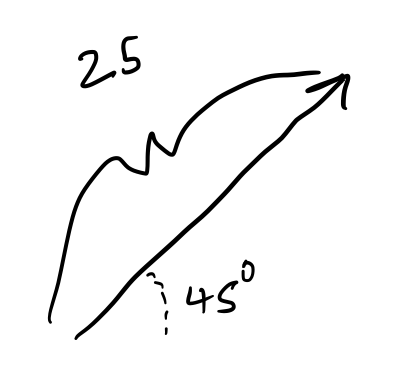
\includegraphics[scale=0.5]{figures_mvc/1stvector}
\end{center}
\end{figure}


 We will denote a vector by a boldface latin letter (either upper or lowercase), such as $\mathbf{x}$. When writing by hand, a more common notation is $\vec{x}$.

\subsubsection{Equality of vectors}
We will now discuss the notion of equivalence of two vectors. Recall first the equivalence of plane figures, say triangles. We consider two distinct triangles. Since the data defining a triangle are the side lengths and interior angle measures, any two triangles related by a transformation which leaves these unchanged represents an equivalent triangle; the only difference between them is the location in the plane. As you learned in basic algebra, any transformation of the plane which preserves lengths and angles can be written as a finite sequence of reflections, translations, and rotations and any two triangles related by such a transformation are said to be \emph{congruent}. 

Since the defining data of a vector is the magnitude and direction, we will agree that

\begin{defn}[Equality of vectors]
Two vectors are equal if they have the same magnitude and direction.	
\end{defn}
That is, two vectors are equal if they are represented by parallel line segments which have the same length and orientation. 

\begin{center}
	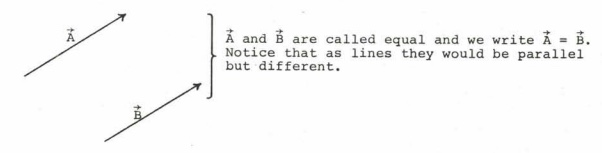
\includegraphics[scale=0.5]{figures_mvc/equal_vectors_new}
\end{center}
If two vectors $\mathbf{x}$ and $\mathbf{y}$ are equal, we will denote this by $\mathbf{x}=\mathbf{y}$.

It is important to note that we have defined equality of vectors so that \emph{location} in space does \emph{not} matter. As line segments, the two parallel arrows are congruent, \footnote{They are congruent simply because they have the same length; the fact that they are parallel or have the same orientation does not matter as far as congruence is concerned.} but still considered distinct due to their difference in location; on the other hand, as \emph{vectors} they are regarded as exactly the same vector. 

\subsection{Vector arithmetic}
We will now define operations involving vectors, whose motivation will come from physics. 

\subsubsection{Vector addition}
The most basic operation one can define on a set is a \emph{binary operation}, which is a rule for combining any two elements in the set to produce a third element in the set. \footnote{More formally, we write this as a map $V \times V \to V$, where $V \times V=\{(v,w) \mid v,w \in V\}$ denotes the set of all ordered pairs of elements of $V$, called the \emph{Cartesian product} of $V$ with itself.} There is a natural binary operation on the set of vectors, which is suggested by the \emph{force table} experiment in mechanics.

\begin{center}
	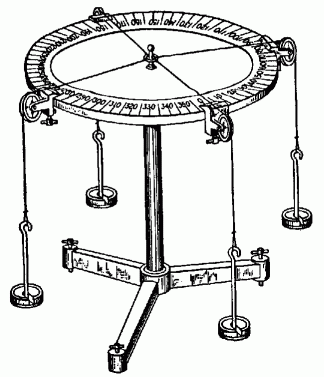
\includegraphics[scale=0.5]{figures_mvc/force_table_experiment_2}
\end{center}

In a force table experiment, strings are tied to a metal ring which is positioned at the center of the table. The strings are then suspended over pulleys which are fixed at known angles, and known masses hung from the ends of the strings. The pull of gravity on a given mass creates tension in the string which pulls on the ring. 

In an experiment in which \emph{two} strings are tied to the ring, the tension in each string gives rise to two forces pulling on the washer in different directions. However, the washer ultimately accelerates in a single direction, which is the direction of the \emph{net} (or \emph{total}) force acting on the ring. The rule for combining the two tension force vectors to produce the net force vector is exactly the binary operation we seek to define. 

To determine the net force, a third string is connected to the ring with mass and pulley position chosen so that the ring is in \emph{static equilibrium} (i.e., it does not move at all under the influence of these three forces). This vector is called the \emph{equilibrant} vector. By Newton's third law, the net force vector (also called the \emph{resultant} vector) is then the \emph{opposite} of the equilibrant vector, that is, it has the same magnitude and is directed along the same line, but with the opposite orientation.

\begin{center}
	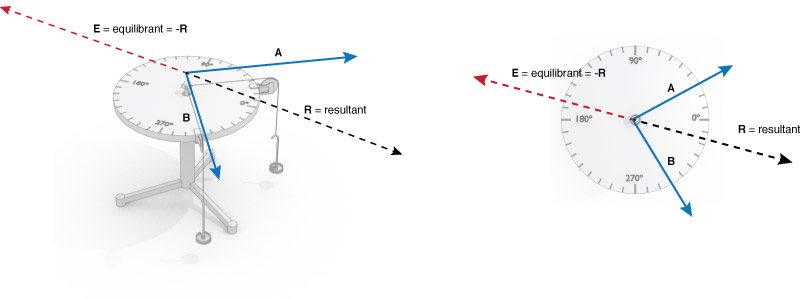
\includegraphics[scale=0.5]{figures_mvc/force-table-equi-res}
\end{center}

 We therefore define the \emph{sum} of two vectors as follows:
 
 \begin{defn}[Vector addition]
 	The \ti{sum} ${\bf v}+{\bf w}$ of two vectors ${\bf v}$ and ${\bf w}$ is the resultant vector of ${\bf v}$ and ${\bf w}$.
 \end{defn}
Note that when the two tension forces are along the \emph{same} direction (e.g., just add another mass on the same string), the resultant vector points in this same direction and has magnitude given by the sum of the magnitudes of the two tension vectors, and hence the addition of ${\bf v}$ and ${\bf w}$ reduces to addition of ordinary numbers in this special case. This is why we have decided to call this binary operation \emph{addition} and to continue to denote it by $+$; it can therefore be thought of as a \emph{generalization} of the ordinary addition of scalars. 
 
In terms of our geometric representation of vectors, the magnitude and direction of ${\bf v}+{\bf w}$ is determined as follows: Since the location of a vector is of no consequence (by our definition of equality of vectors), we may position the two vectors so that their initial points coincide. Then ${\bf v}$ and ${\bf w}$ form adjacent sides of a parallelogram, and the vector ${\bf v}+{\bf w}$ is the diagonal of the parallelogram, directed from the common initial point of ${\bf v}$ and ${\bf w}$ to the opposite vertex of the parallelogram, as shown below.	
\begin{center}
	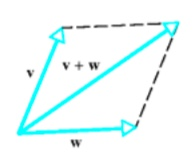
\includegraphics[scale=0.5]{figures_mvc/parallelogram_rule}
\end{center}
This is called the \ti{parallelogram rule} for vector addition. Since the opposite sides of a parallelogram are congruent and parallel, we can equivalently view ${\bf v}+{\bf w}$ as the result of positioning the initial point of ${\bf w}$ at the terminal point of ${\bf v}$ and drawing the arrow connecting the initial point of ${\bf v}$ to the terminal point of ${\bf w}$.

	\begin{center}
	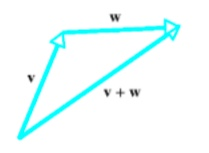
\includegraphics[scale=0.5]{figures_mvc/tip_to_tail}
\end{center}


This is called the \ti{triangle rule} or \ti{``tip to tail" rule} for vector addition. These two points of view are related by \ti{parallel translation}. To go from the first point of view to the second, we translate the initial point of ${\bf w}$ along ${\bf v}$, keeping ${\bf w}$ parallel to its original direction at all times. Accordingly, ${\bf v}+{\bf w}$ is also called the \ti{translation of ${\bf w}$ by ${\bf v}$}.
\begin{center}
	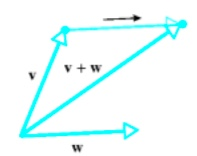
\includegraphics[scale=0.5]{figures_mvc/translation_of_v_by_w}
\end{center}

\begin{example}
There is another physical interpretation of this addition rule which agrees with our intuition. Suppose a person walks 10 steps in a north-easterly direction, and then turns and walks another 5 steps to the east. The vector $\mathbf{v}$ then represents his \emph{displacement} from his initial position, with the length of $\mathbf{v}$ being his distance from where he started, and the direction of $\mathbf{v}$ pointing in the direction in which he moved. Similarly, the vector $\mathbf{w}$ represents his displacement from his position after he traveled along the vector $\mathbf{v}$. Their sum, added according to the tip to tail rule, is his \emph{total} displacement from his initial position.	
\end{example}

Let us now use this geometric picture to determine the properties of vector addition. Recall that the addition operation defined on the set of real numbers satisfies the following properties: \footnote{Any set $G$ on which there is a binary operation $*$ which satisfies the first three of these properties is said to form a \emph{group} under $*$. One also says that $(G,*)$ is a group, or just that $G$ is a group if $*$ is understood. If the fourth property (commutativity) also holds, $G$ is said to form a \emph{commutative} (or \emph{abelian}) under $*$.}
\begin{enumerate}[(i)]
	\item Associativity: $(x+y)+z=x+(y+z)$ for all $x,y,z \in \mathbb{R}$.
	\item Existence of an additive identity: $\mathbb{R}$ contains an element 0 such that $0+x=x$ for every $x \in \mathbb{R}$.
	\item Existence of additive inverses: For every $x \in \mathbb{R}$, there exists and element $y \in \mathbb{R}$ such that $x+y=0$.
	\item Commutativity: $x+y=y+x$ for all $x,y \in \mathbb{R}$.
\end{enumerate}
We now consider each of these in turn. We consider commutativity first, since it is the simplest to analyze.

\begin{prop}[Vector addition is commutative]
	Vector addition is commutative. That is, 
	\begin{align*}
		{\bf v}+{\bf w}={\bf w}+{\bf v}
	\end{align*}
	for any two vectors ${\bf v}$ and ${\bf w}$, since each of these is the diagonal of the parallelogram whose edges are formed by $\mathbf{v}$ and $\mathbf{w}$.
\end{prop}

\begin{pf}
	We see from the two diagrams below that the translation of ${\bf w}$ by ${\bf v}$ is the same vector as the translation of ${\bf v}$ by ${\bf w}$.
\begin{center}
	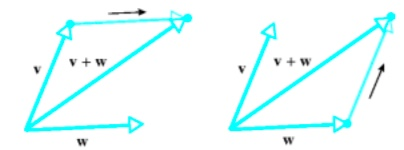
\includegraphics[scale=0.5]{figures_mvc/equivalence_of_vector_addition}
\end{center}

\end{pf}

\begin{prop}[Vector addition is associative]
	Vector addition is associative. That is, for any three vectors ${\bf u}, {\bf v},$ and ${\bf w}$, we have
	\begin{align*}
		{\bf u}+({\bf v}+{\bf w})=({\bf u}+{\bf v})+{\bf w}
	\end{align*}
We therefore denote both expressions by ${\bf u}+{\bf v}+{\bf w}$. 
\end{prop}

\begin{pf}
One can construct ${\bf u}+{\bf v}+{\bf w}$ by placing the vectors ``tip to tail" in succession and then drawing the vector from the initial point of ${\bf u}$ to the terminal point of ${\bf w}$. If the three vectors lie in the same plane, one can verify associativity from the diagram below.
\end{pf}

\begin{center}
	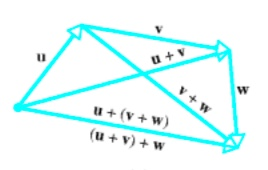
\includegraphics[scale=0.5]{figures_mvc/associativity_of_vector_addition}
\end{center}

If the three vectors do not all lie in the same plane, then when placed at the same initial point the vectors ${\bf u}, {\bf v},$ and ${\bf w}$ from adjacent edges of a \emph{parallelepiped}. \footnote{A parallelepiped is a polygon whose faces are parallelograms, with each pair of opposite sides parallel.} Translating these vectors and adding tip to tail, we see that ${\bf u}+{\bf v}+{\bf w}$ is the diagonal of this parallelepiped.

\begin{center}
	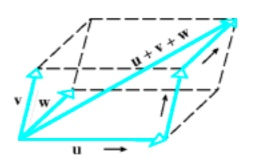
\includegraphics[scale=0.5]{figures_mvc/volume_of_parallelepiped_vectors}
\end{center}

\begin{cor}
The sum ${\bf v}_1+{\bf v}_2+\cdots + {\bf v}_k$ is independent of how the expression is bracketed.	
\end{cor}

\begin{pf}
We postpone the proof until we discuss vectors in coordinates in section \ref{sec:coords}, as the geometry is very complicated and difficult to analyze. In coordinates, this is seen to hold as a simple consequence of the fact that it holds for real numbers.
\end{pf}

Let us now check whether there is a vector which plays the role of an additive identity. That is, given any vector ${\bf b}$, is there a vector ${\bf 0}$ such that ${\bf b}+{\bf 0}={\bf b}$? Let us suppose there is such a vector ${\bf 0}$ and denote its magnitude by $r$. Let us now add ${\bf 0}$ to ${\bf b}$ by the tip-to-tail method. Since ${\bf 0}$ has magnitude $r$, ${\bf b}+{\bf 0}$ must lie on a circle of radius $r$ centered on the tip of ${\bf b}$. However, the condition ${\bf b}+{\bf 0}={\bf b}$ means that ${\bf b}+{\bf 0}$ must have the same magnitude and direction as ${\bf b}$, and there is no point on the circle for which this is true. This shows that there is no such vector ${\bf 0}$ with nonzero length. 
\begin{center}
	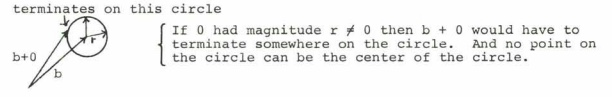
\includegraphics[scale=0.5]{figures_mvc/b_plus_zero_circle}
\end{center}

A vector of length zero, does not have a defined direction. Thus, there is a unique vector which acts as an additive identity with respect to vector addition.

\begin{defn}[The zero vector]
	The zero vector, which we denote by ${\bf 0}$, is the unique vector of magnitude zero.
\end{defn}

Finally, we want to investigate whether every vector has an additive inverse. That is, we want to determine if, when given any vector ${\bf a}$, we can find another vector ${\bf b}$ such that ${\bf a}+{\bf b}={\bf 0}$. Since the zero vector has zero length and since we add vectors from ``tip to tail", it follows that if ${\bf a}+{\bf b}={\bf 0}$, then the tail of ${\bf a}$ and the tip of ${\bf b}$ must coincide. Thus, any vector $\mathbf{a}$ has a \emph{unique} inverse, which we denote by $-\mathbf{a}$.   
\begin{center}
	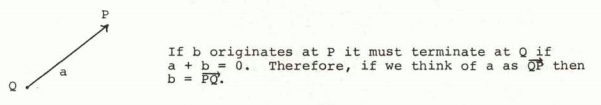
\includegraphics[scale=0.5]{figures_mvc/a_plus_b_equals_zero}
\end{center} 
\begin{defn}[Inverse of a vector]
The additive inverse of a vector ${\bf a}$ is the unique vector $-\mathfrak{a}$, which has the same magnitude as $\mathbf{a}$ and opposite orientation.
\end{defn}
In analogy with the equation $x+(-x)=0$ for real numbers, we denote the additive inverse of ${\bf a}$ by $-{\bf a}$, so that ${\bf a}+(-{\bf a})={\bf 0}$ for any vector ${\bf a}$. We may again agree, as in the case of numerical addition, to abbreviate ${\bf a}+(-{\bf b})$ as ${\bf a}-{\bf b}$, which allows us to define vector subtraction:

\begin{defn}[Vector subtraction]\label{def:vector_subtraction}
	The difference ${\bf a}-{\bf b}$ of two vectors ${\bf a}$ and ${\bf b}$ is the sum
	\begin{align*}
		{\bf a}-{\bf b}={\bf a}+(-{\bf b}).
	\end{align*}
\end{defn}
From this definition, we may view vector subtraction geometrically as follows: To form ${\bf a}-{\bf b}$,
\begin{enumerate}[(1)]
	\item Obtain $(-{\bf b})$ from ${\bf b}$ by reversing the direction of ${\bf b}$.
	\item Add ${\bf a}$ and $(-{\bf b})$ in the usual way, by placing the tail of $(-{\bf b})$ at the tip of ${\bf a}$. \footnote{Like numerical subtraction, vector subtraction is \ti{not} commutative, so the order matters here.}
\end{enumerate}

\begin{center}
	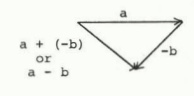
\includegraphics[scale=0.5]{figures_mvc/a_minus_b}
\end{center}

\begin{exercise}
Show that if $\mathbf{a}$ and $\mathbf{b}$ are placed such that their initial points coincide, then $\mathbf{x}={\bf a}-{\bf b}$ is the vector which extends from the tip of ${\bf b}$ to the tip of ${\bf a}$.
	\begin{center}
		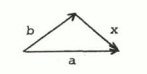
\includegraphics[scale=0.5]{figures_mvc/b_plus_x_equals_a}
	\end{center}
\end{exercise}

In this section we have shown that our definition of vector addition satisfies the same properties as ordinary addition of real numbers. That is, the additive structures are exactly the same for vectors as for numbers. \footnote{To state this more formally, they both form an abelian group.} Therefore, any results that hold for numbers also hold for vectors, for exactly the same reasons. For example,

\begin{thm}[Cancellation law]
	If ${\bf a}, {\bf b},$ and ${\bf c}$ are vectors such that ${\bf a}+{\bf b}={\bf a}+{\bf c}$, then ${\bf b}={\bf c}$. 
\end{thm}

\begin{pf}
The proof for real numbers is as follows: let $x,y,z$ be real numbers such that 
\begin{align*}
	x+y=x+z
\end{align*}
Adding $-x$ to both sides of this equation, we have
\begin{align*}
	-x+(x+y)&=-x+(x+z) \\
	(-x+x)+y&=(-x+x)+z \text{ (since $+$ is associative)} \\
	0+y&=0+z \text{ (since $-x$ is the inverse of $x$)} \\
	y&=z \text{ (since $0$ is the additive identity)}
\end{align*}
Since addition of vectors obeys exactly the same properties as addition of real numbers, this same proof holds for vectors simply by drawing arrows over $x,y$ and $z$!
\end{pf}

\subsubsection{Scalar multiplication}
In physics, we observe that an unbalanced force on a body causes an acceleration in the direction of the force. It is also observed that the magnitude of acceleration of different bodies, when subjected to the same force, varies according to their mass. These observations are formalized in Newton's second law of motion
\begin{equation}
	{\bf F}=m{\bf a}.
\end{equation}
On the right side of this equation, we see a new operation: the product of a scalar and a vector. 

\begin{defn}[Scalar multiplication]
Let $\mathbf{v}$ be a vector and $k$ a scalar. The \emph{scalar multiple} of ${\bf v}$ by $k$ is a vector $\mathbf{w}$, defined as follows:
\begin{itemize}
	\item The length of ${\bf w}$ is $|k|$ times the length of ${\bf v}$. If $|k|=0$, then $\mathbf{w}$ is the zero vector.
	\item $\mathbf{w}$ is parallel to $\mathbf{v}$.
	\item If $k>0$, then $\mathbf{w}$ has the same orientation as $\mathbf{v}$. If $k<0$, then $\mathbf{w}$ and $\mathbf{v}$ have opposite orientation.
\end{itemize}
If $\mathbf{w}$ is the scalar multiple of $\mathbf{v}$ by $k$, we write $\mathbf{w}=k\mathbf{v}$. \footnote{Note that scalar multiplication is not a binary operation on $V$, since it does not take two vectors to a vector, but rather a scalar and a vector to a vector. More formally, scalar multiplication is a map $\R \times V \to V$.}
\end{defn}

\begin{example}
The vector $2{\bf v}$ has the same direction as ${\bf v}$ but twice its length, while $-2{\bf v}$ is oppositely directed to ${\bf v}$ and twice its length. 

\begin{figure}[h]
	\begin{center}
	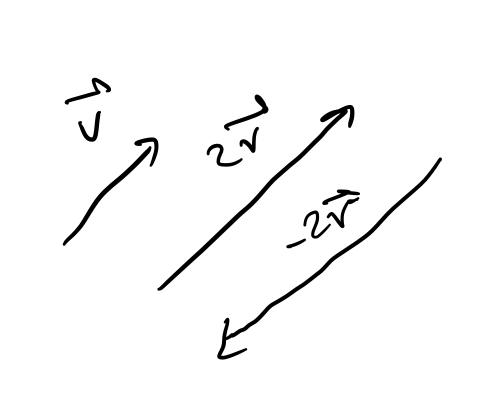
\includegraphics[scale=0.4]{figures_mvc/v2v}
\end{center}
\end{figure}
\end{example}
\newpage
\begin{thm}[Properties of scalar multiplication]\label{thm:properties_of_scalar_multiplication}
For any scalars $c,d$ and vectors ${\bf v}, {\bf w}$, 
	\begin{enumerate}[(i)]
		\item $0{\bf v}={\bf 0}$,
		\item $1{\bf v}={\bf v}$,
		\item $(-1){\bf v}=-{\bf v}$,
		\item $(c+d){\bf v}=c{\bf v}+d{\bf v}$,
		\item $c({\bf v}+{\bf w})=c{\bf v}+c{\bf w}$,
		\item $(dc){\bf v}=c(d{\bf v})$.
	\end{enumerate}
\end{thm}

\begin{pf}
	We will prove pars (i) and (ii) and leave the rest as an exercise. In each case, we need to show that the vector on the left hand side has the same magnitude and direction as the vector on the right hand side. 
	\begin{enumerate}[(i)]
		\item The vector $1\mathbf{v}$ has length $|1|=1$ times the length of $\mathbf{v}$, and therefore has the same length as $\mathbf{v}$. The vector $1\mathbf{v}$ is parallel to $\mathbf{v}$, and since $1>0$ it has the same orientation as $\mathbf{v}$. This shows $1 \mathbf{v}$ has the same magnitude and direction as $\mathbf{v}$, and therefore $1 \mathbf{v}=\mathbf{v}$.
		\item The length of $0\mathbf{v}$ is zero times the length of $\mathbf{v}$, which is zero. Hence, $0\mathbf{v}$ is the zero vector. 
	\end{enumerate} 
\end{pf}

\begin{exercise}
Prove parts (iii)-(vi) of Theorem \ref{thm:properties_of_scalar_multiplication}.	
\end{exercise}

The diligent reader who has worked through the exercises in this section has most likely found many of them to be quite tedious. While the geometric picture of vectors we have developed in this section will be essential for visualization purposes, it is indeed far from optimal for practical computations. This situation will be rectified in the next section by introducing Cartesian coordinate systems in which to describe vectors. \footnote{As should be familiar from freshman geometry, a coordinate system is called Cartesian (or rectangular) if its coordinate axes are all mutually perpendicular.} As we will see, all properties we deduced geometrically in this section will be seen to hold as simple consequences of the properties of real numbers. Despite this simplification of computations, it is important to remember that vectors are geometrical objects whose properties (length and magnitude) do not depend on any particular coordinate system which we may use to describe them.

\subsection{Vectors in coordinate systems}\label{sec:coords}
Let us now describe vectors with respect to a Cartesian coordinate system.

\subsubsection{Vectors in one dimension}
A one-dimensional Cartesian coordinate system is provided by the real number line. Consider a nonzero vector inside the real line; that is, an arrow originating at some point $x_1$ and terminating at a distinct point $x_2$. \footnote{The zero vector has length zero and is therefore just a point.} This vector can point in only one of two directions: either left or right, depending on whether $x_2<x_1$, or $x_1<x_2$, respectively.  Since the location of the vector does not matter, we are free to consider the vector to have initial point at the origin. In this case, the vector originates at the origin, and terminates at some point $x$. The length of the vector is then $|x|$, and its orientation is determined by the sign of $x$, which we denote by $\sgn(x)$, which can be written as $\sgn(x)=\frac{x}{|x|}$. 
\begin{exercise}
	Prove that 
\begin{align*}
	\frac{x}{|x|}=\begin{cases}
		+1, &\text{ if } x>0, \\
		-1, &\text{ if } x<0. \\
	\end{cases}
\end{align*}
\end{exercise}

If we have two such vectors terminating at $x_1$ and $x_2$, respectively, then these vectors are equal if and only if $|x_1|=|x_2|$ and $\sgn(x_1)=\sgn(x_2)$. Since for any $x \neq 0$, we can write
\begin{align*}
	x&=\frac{x}{|x|}|x|\\
	&=\sgn(x)|x|,
\end{align*} 
these vectors are equal if and only if $x_1=x_2$. This shows that there is a 1-1 correspondence between vectors in one-dimension and real numbers, with the correspondence given by
\begin{align*}
	x \leftrightarrow \mathbf{x}=(\sgn(x),|x|).
\end{align*}
We see that there is no essential difference between vectors in one dimension and scalars.

\subsubsection{Vectors in two dimensions}
A two-dimensional Cartesian coordinate system is given by $\R^2=\{(x,y) \mid x,y \in \R\}$. Each point $(x,y) \in \R^2$ specifies the coordinates of a point in a plane. Again, we are free to parallel translate all vectors so that their initial point is at the origin. If the terminal point of such a vector $\mathbf{x}$ is $(x,y)$, then the magnitude of $\mathbf{x}$, which we denote by $||\mathbf{x}||$, \footnote{We use double bars to denote the magnitude of a vector to distinguish this from the absolute value of a real number. Note that, when $\mathbf{x}$ is one dimensional, then $||\mathbf{x}||=\sqrt{x^2}=|x|$.} is given by the Pythagorean theorem 
\begin{align*}
	||\mathbf{x}||=\sqrt{x^2+y^2}.
\end{align*}
We specify the direction of this vector by giving the angle $\theta$ with respect to the positive $x$-axis, which is given by
\begin{align*}
	\theta=\tan^{-1}\left(\frac{y}{x}\right).
\end{align*}
where $\theta \in [0,2\pi)$. Note that this is just the usual change of coordinates from Cartesian to polar coordinates. Since two vectors are equal if and only if $||\mathbf{x_1}||=||\mathbf{x_2}||$ and $\theta_1=\theta_2$, inverting the formulas above
\begin{align*}
	x&=||\mathbf{x}||\cos \theta, \\
	y&=||\mathbf{x}||\sin \theta,
\end{align*}
shows that $(||\mathbf{x}_1||,\theta_1)=(||\mathbf{x}_2||,\theta_2)$ implies $(x_1,y_1)=(x_2,y_2)$. Thus, two-dimensional vectors are in 1-1 correspondence with points in $\R^2$. The coordinates of the end point of the vector are called the \emph{components} of the vector. We will write a two-dimensional vector $\mathbf{v}$ in terms of its components by writing $\mathbf{v}=(v_1,v_2)$. As we have just seen, this expression for $\mathbf{v}$ in terms of its coordinates is unique.

\subsubsection{Vectors is three dimensions}
A three-dimensional Cartesian coordinate system is shown below. 
\begin{center}
	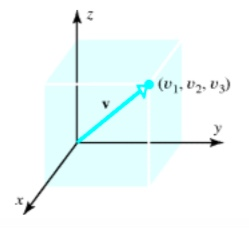
\includegraphics[scale=0.5]{figures_mvc/components}
\end{center}
The coordinate axes are labeled $x,y,$ and $z$, and are arranged such that if you take your right hand and curl your fingers from the positive $x$-axis toward the positive $y$-axis, your thumb points along the positive $z$-axis. Such a coordinate system is called \emph{right-handed}. Again, we find the set of all vectors in three dimensions is in 1-1 correspondence with the set $\R^3=\{(x,y,z) \mid x,y,z \in \R\}$. If $\varphi$ is the angle the vector makes with the positive $z$-axis and $\theta$ is the angle the projection of the vector onto the xy-plane makes with the positive $x$-axis (i.e., it is the usual polar angle in the plane), then the direction of a vector $\mathbf{x}$ is specified by the two angles $(\varphi,\theta)$, where we take $\varphi \in [0,\pi], \theta \in [0,2\pi)$. A little trigonometry shows that the correspondence between $(||\mathbf{x}||,(\varphi,\theta))$ and $(x,y,z)$ is given by
\begin{align}\label{eq:x_spher}
	x&=||\mathbf{x}||\sin \varphi \cos \theta, \\ \label{eq:y_spher}
	y&=||\mathbf{x}||\sin \varphi \sin \theta, \\ \label{eq:z_spher}
	z&=||\mathbf{x}||\cos \varphi. \\
\end{align}
\begin{figure}[h]
\begin{center}
	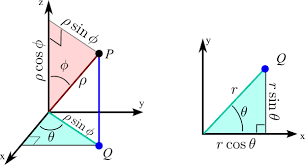
\includegraphics[scale=0.8]{figures_mvc/speric_coor}
\end{center}
\end{figure}
\begin{exercise}
Work out these formulas from the diagram.	
\end{exercise}


As in two-dimensions, we write a three-dimensional vector $\mathbf{v}$ in terms of its components as $\mathbf{v}=(v_1,v_2,v_3)$, and this expression is unique. From the formulas \eqref{eq:x_spher}-\eqref{eq:z_spher}, we see that the length of a vector $\mathbf{v}$ is given by an obvious generalization of the Pythagorean formula
\begin{equation}\label{eq:norm}
	||\mathbf{v}||=\sqrt{v_1^2+v_2^2+v_3^2}.
\end{equation}

\begin{exercise}
	Use the formulas \eqref{eq:x_spher}-\eqref{eq:z_spher} above to prove this.
\end{exercise}


\subsubsection{Vector arithmetic in coordinates}
We now derive the rule for vector addition in terms of components. Given vectors $\mathbf{v}$ and $\mathbf{w}$, we wish to find the components of $\mathbf{v}+\mathbf{w}$. According to the tip-to-tail rule, the $\mathbf{v}+\mathbf{w}$ is given by translating the vector $\mathbf{w}$ so that its initial point coincides with the terminal point of $\mathbf{v}$. This translation moves the $x$-coordinate of $\mathbf{w}$ by $v_1$ units in the $x$-direction, the $y$-coordinate by $v_2$ units in the $y$-direction, and the $z$-coordinate by $v_3$ units in the $z$-direction. That is, 
\begin{align*}
	(w_1,w_2,w_2) \mapsto (v_1+w_1,v_2+w_2,v_3+w_3)
\end{align*}
Thus, the coordinates of the endpoint of $\mathbf{v}+\mathbf{w}$ are given by
\begin{align*}
	\mathbf{v}+\mathbf{w}=(v_1+w_1,v_2+w_2,v_3+w_3).
\end{align*}
\begin{defn}[Vector addition in components]\label{def:vector_addition}
	In terms of components, the rule for vector addition is given by:
\begin{enumerate}[(i)]
	\item Vectors in one-dimension:
	\begin{align*}
		(v_1)+(w_1)=(v_1+w_1)
	\end{align*}
	\item Vectors in two-dimensions:
	\begin{align*}
		(v_1,v_2)+(w_1,w_2)=(v_1+w_1,v_2+w_2).
	\end{align*}
	\item Vectors in three-dimensions:
	\begin{align*}
		(v_1,v_2,v_3)+(w_1,w_2,w_3)=(v_1+w_1,v_2+w_2,v_3+w_3).
	\end{align*}
\end{enumerate}
\end{defn}

This formula is illustrated in the diagram on the left in Figure \ref{fig:vector_operations}.

\begin{example}
Let $\mathbf{v}=(1,2,3)$ and $\mathbf{w}=(-3,1,7)$. Then 
\begin{align*}
	\mathbf{v}+\mathbf{w}=(-2,3,10).
\end{align*}	
\end{example}


\begin{exercise}
	\begin{enumerate}[(a)]
		\item Use the formula in Definition \ref{def:vector_addition} to show that vector addition is commutative.
		\item Use the formula in Definition \ref{def:vector_addition} to show that vector addition is associative.
		\item What are the components of the zero vector?
		\item Given a vector $\mathbf{v}=(v_1,v_2,v_3)$, what are the components of $-\mathbf{v}$ (the additive inverse of $\mathbf{v}$)?
	\end{enumerate}
\end{exercise}
\newpage
\begin{prop}\label{prop:scalar_multiple_formula}
If $\mathbf{v}=(v_1,v_2,v_3)$ is a vector and $k$ a scalar, then the components of the scalar multiple $k\mathbf{v}$ of $\mathbf{v}$ by $k$ are given by
\begin{enumerate}[(i)]
	\item Vectors in one dimension:
	\begin{align*}
		k(v_1)&=(kv_1) \\
	\end{align*}
	\item Vectors in two dimensions:
	\begin{align*}
		k(v_1,v_2)&=(kv_1,kv_2) \\
	\end{align*}
	\item Vectors in three dimensions:
	\begin{align*}
		k(v_1,v_2,v_3)&=(kv_1,kv_2,kv_3)
	\end{align*}
\end{enumerate}	
\end{prop}

\begin{exercise}
	\begin{enumerate}[(a)]
		\item Prove these formulas for vectors in one and two dimensions.
		\item Use this formula to prove that $||k\mathbf{v}||=|k| \cdot ||\mathbf{v}||$ for vectors in three dimensions.
		\item Show that if $k>0$, then $k\mathbf{v}$ has the same direction as $\mathbf{v}$. \footnote{This formula still holds if $k<0$, but checking this case involves some care since $\varphi$ must stay in the range $[0,\pi)$ and $\theta$ in $[0,2\pi)$.} 
	\end{enumerate}
\end{exercise}

\begin{example}
Let $\mathbf{v}=(1,2,3)$ and $k=3$. Then
\begin{align*}
	k\mathbf{v}=(3,6,9).
\end{align*}	
\end{example}

The formula in \eqref{prop:scalar_multiple_formula} is illustrated in the diagram on the right in Figure \ref{fig:vector_operations}.


\begin{exercise}
Use the formula in Proposition \eqref{prop:scalar_multiple_formula} to prove Theorem \eqref{thm:properties_of_scalar_multiplication}.	
\end{exercise}

\begin{figure}\label{fig:vector_operations}
	\begin{center}
	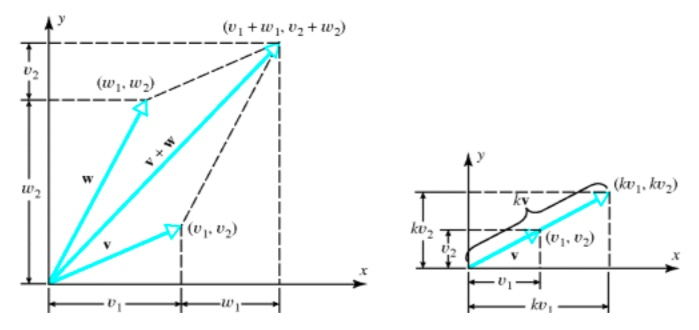
\includegraphics[scale=0.5]{figures_mvc/vector_operations}
\end{center}	
\caption{Vector operations in components.}
\end{figure}

\begin{exercise}
Prove that if $\mathbf{v}=(v_1,v_2,v_3)$ and $\mathbf{w}=(w_1,w_2,w_3)$, then
\begin{align*}
	\mathbf{v}-\mathbf{w}=(v_1-w_1,v_2-w_2,v_3-w_3).
\end{align*}	
\end{exercise}

 The distance between two points $(v_1,v_2,v_3)$ and $(w_1,w_2,w_3)$ in $\mathbb{R}^3$ is therefore given by
\begin{align*}
	||\mathbf{v}-\mathbf{w}||=\sqrt{(v_1-w_1)^2+(v_2-w_2)^2+(v_3-w_3)^2}.
\end{align*}

\begin{example}
\begin{enumerate}[(a)]
	\item Find the components of the vector $\overrightarrow{P_1P_2}$ with initial point $P_1(2,-1,4)$ and terminal point $P_2(7,5,-8)$.
	\item Find the distance between $P_1(2,-1,4)$ and $P_2(7,5,-8)$.
\end{enumerate}	
\end{example}

{\color{red} \flushleft {\bf Solution:} 
\begin{enumerate}[(a)]
	\item The components of $\overrightarrow{P_1P_2}$ are given by
	\begin{align*}
		\overrightarrow{P_1P_2}=(7-2,5-(-1),-8-4)=(5,6,-12)
	\end{align*}
	\item The distance between $P_1$ and $P_2$ is 
	\begin{align*}
		||\overrightarrow{P_1P_2}||=\sqrt{5^2+6^2+(-12)^2}=\sqrt{205}.
	\end{align*}
\end{enumerate}}

\subsubsection{Unit vectors}
\begin{defn}[Unit vector]
	A \emph{unit vector} is a vector of unit length. That is, a vector ${\bf v}$ such that $||{\bf v}||=1$.
\end{defn}

\begin{prop}[Normalizing a vector]
	If ${\bf v}\neq 0$, then ${\bf v}/||{\bf v}||$ is a unit vector in the direction of ${\bf v}$. The unit vector ${\bf v}/||{\bf v}||$ is often denoted ${\bf \hat{v}}$ and the process of forming ${\bf \hat{v}}$ from ${\bf v}$ is called \ti{normalizing} ${\bf v}$.
\end{prop}

\begin{pf}
Since ${\bf v}\neq 0$, $||{\bf v}|| \neq 0$, so we can multiply ${\bf v}$ by $1/||{\bf v}||$. Computing the length of $||\frac{{\bf v}}{||{\bf v}||}||$, we see that 
\begin{align*}
	||\frac{{\bf v}}{||{\bf v}||}||&=\frac{||{\bf v}||}{||{\bf v}||}=1,
\end{align*} 
hence ${\bf v}/||{\bf v}||$ is a unit vector. Since ${\bf v}/||{\bf v}||$ is a scalar multiple of ${\bf v}$ (by $k=1/||{\bf v}||$) it is parallel to ${\bf v}$, and since $k>0$, ${\bf v}/||{\bf v}||$ has the same orientation as $\mathbf{v}$.
\end{pf}

\begin{example}
	We can express any nonzero vector ${\bf v}$ as a product of its magnitude and direction by means of the formula \footnote{Note that this is a generalization of the formula $x=|x|\frac{x}{|x|}$ for a nonzero real number $x$.}
	\begin{align*}
		{\bf v}=||{\bf v}||\frac{{\bf v}}{||{\bf v}||}.
	\end{align*}
	For example, taking ${\bf v}=(1,-2,3)$,
	\begin{align*}
		||{\bf v}||=\sqrt{1^2+(-2)^2+3^2}=\sqrt{14}
	\end{align*}
	and thus
	\begin{align*}
		{\bf v}=\sqrt{14}(\frac{1}{\sqrt{14}},\frac{-2}{\sqrt{14}},\frac{3}{\sqrt{14}}).
	\end{align*}
\end{example}


\begin{defn}[Standard unit vectors]
	 The \ti{standard unit vectors} for $\mathbb{R}^3$ are the vectors
	\begin{align*}
		{\bf i}&=(1,0,0), \\
		{\bf j}&=(0,1,0), \\
		{\bf k}&=(0,0,1). \\
	\end{align*}
These vectors are unit vectors pointing along the $x$-, $y$-, and $z$-axes, respectively. \footnote{The standard unit vectors $({\bf i},{\bf j},{\bf k})$ are also commonly denoted as $({\bf e}_1, {\bf e}_2, {\bf e}_3)$ or $({\bf \hat{x}}, {\bf \hat{y}}, {\bf \hat{z}})$.}	
\end{defn}
Using the standard unit vectors, we may write the vector ${\bf v}=(v_1,v_2,v_3)$ as $${\bf v}=v_1{\bf i}+v_2{\bf j}+v_3{\bf k}.$$
A sum of this form is said to be a \emph{linear combination} of the vectors ${\bf i},{\bf j},{\bf k}$. You should be comfortable working with both expressions for a vector $\mathbf{v}$ in terms of its components.

\begin{example}
Find a unit vector in the direction of the vector from $P_1(1,0,1)$ to $P_2(3,2,0)$.
\end{example}

{\color{red} \flushleft {\bf Solution:}
We find $\overrightarrow{P_1P_2}$ and normalize:
\begin{align*}
	\overrightarrow{P_1P_2}&=(3-1,2-0,0-1)=(2,2,-1), \\
	||\overrightarrow{P_1P_2}||&=\sqrt{2^2+2^2+(-1)^2}=3, \\
\end{align*}
and therefore the desired unit vector is given by
\begin{align*}
	\frac{\overrightarrow{P_1P_2}}{||\overrightarrow{P_1P_2}||}=(\frac{2}{3},\frac{2}{3},-\frac{1}{3}).
\end{align*}}

\begin{example}
Find a vector 6 units long in the direction of ${\bf v}=(2,2,-1)$.	
\end{example}

{\color{red} \flushleft {\bf Solution:}
The vector we want is 
\begin{align*}
6\frac{{\bf v}}{||{\bf v}||}=6\frac{(2,2,-1)}{\sqrt{2^2+2^2+(-1^2)}}=6\frac{(2,2,-1)}{3}=(4,4,-2).	
\end{align*}
}

\subsubsection{The dot product}
Two nonzero vectors ${\bf u}$ and ${\bf v}$ positioned so that their initial points coincide determine an angle $\theta \in [0,\pi]$, which is the angle between the two vectors.
\begin{center}
	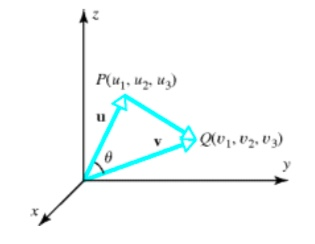
\includegraphics[scale=0.5]{figures_mvc/angle_uv}
\end{center}
Note that the information about $\theta$ is encoded in ${\bf u}-{\bf v}$, since if we fix the magnitudes of ${\bf u}$ and ${\bf v}$ and open the angle, then ${\bf u}-{\bf v}$ will also change. The fundamental relation satisfied by ${\bf u}, {\bf v}$ and $\theta$ is the law of cosines, which says that if ${\bf w}={\bf u}-{\bf v}$, then
\begin{equation}\label{eq:law_of_cosines}
	||{\bf w}||^2=||{\bf u}||^2+||{\bf v}||^2-2||{\bf u}|| \ ||{\bf v}||\cos \theta. 
\end{equation}
Let us make the following definition.
\begin{defn}[Dot product]
	The \emph{dot product} of two nonzero vectors ${\bf u}$ and ${\bf v}$ is defined by
	\begin{equation}\label{eq:dot_product_def}
		{\bf u}\cdot {\bf v}=||{\bf u}|| \ ||{\bf v}||\cos\theta.
	\end{equation} 
\end{defn}
The angle between two vectors ${\bf u}$ and ${\bf v}$ is then given in terms of their dot product by
\begin{equation}\label{eq:angle_uv}
	\theta=\cos^{-1}\left(\frac{{\bf u}\cdot {\bf v}}{||{\bf u}|| \ ||{\bf v}||}\right),
\end{equation}	
and we see that
\begin{itemize}
	\item $\theta$ is acute if ${\bf u} \cdot {\bf v} > 0$.
	\item $\theta$ is obtuse if ${\bf u} \cdot {\bf v} < 0$.
	\item $\theta$ is right if ${\bf u} \cdot {\bf v} = 0$.
\end{itemize}

Since the dot product takes as input two vectors and returns a scalar, it is also called the \emph{scalar product}. Note that from Eq. \eqref{eq:law_of_cosines}, we can write ${\bf u}\cdot {\bf v}$ in terms of magnitudes only, as 
\begin{equation}\label{eq:dot_product_magnitudes}
	{\bf u}\cdot {\bf v}=\frac{||{\bf u}||^2+||{\bf v}||^2-||{\bf u}-{\bf v}||^2}{2}.
\end{equation}
Note that, unlike \eqref{eq:dot_product_def}, the right hand side of \eqref{eq:dot_product_magnitudes} is defined if either $\mathbf{u}=\mathbf{0}$ or $\mathbf{v}=\mathbf{0}$, in which case $\mathbf{u}\cdot \mathbf{v}=0$. Thus, we define the dot product of any vector with the zero vector to be zero:
\begin{align}
	\mathbf{v}\cdot \mathbf{0}=0
\end{align}
for every vector $\mathbf{v}$.

Since \eqref{eq:dot_product_magnitudes} involves only lengths of segments and angles between segments, it holds in \emph{all} coordinate systems. However, it takes a particularly simple form in Cartesian coordinates. Writing out the norm of each vector in terms of its components gives

\begin{align}\label{eq:dot_mess}
	{\bf u}\cdot {\bf v}&=\frac{u_1^2+u_2^2+u_3^2+v_1^2+v_2^2+v_3^2-(u_1-v_1)^2-(u_2-v_2)^2-(u_3-v_3)^2}{2}
\end{align}
Expanding the binomials and cancelling like terms, we find
\begin{equation}\label{eq:dot_simplified}
	{\bf u}\cdot {\bf v}=u_1v_1+u_2v_2+u_3v_3.
\end{equation}

\begin{exercise} 
Simplify equation \eqref{eq:dot_mess} to obtain \eqref{eq:dot_simplified}. 	
\end{exercise}


\begin{example}
Compute the angle between the vectors ${\bf u}=(0,0,3)$ and ${\bf v}=(\sqrt{2},0,\sqrt{2})$.	
\end{example}

{\color{red} \flushleft {\bf Solution:} The angle between these vectors is
\begin{align*}
	\theta=\cos^{-1}\left(\frac{0(\sqrt{2}+0(0)+3(\sqrt{2}))}{3(2)}\right)=\cos^{-1}\left(\frac{1}{\sqrt{2}}\right)=\frac{\pi}{4}.
\end{align*}}

\begin{example}
	Find the angle between a diagonal of a cube and one of its edges.
\end{example}

{\color{red} \flushleft {\bf Solution:}
Let $s$ be the length of an edge and place the cube in the first octant so that one vertex is at the origin and two edges are along the $x$- and $y$-axes.
\begin{center}
	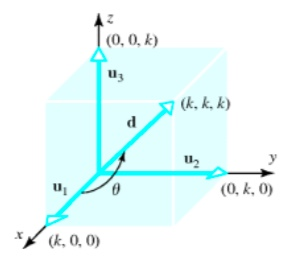
\includegraphics[scale=0.5]{figures_mvc/cube_coordinates}
\end{center}
If we let ${\bf u}_1=(s,0,0), {\bf u}_1=(0,s,0)$, and ${\bf u}_3=(0,0,s)$, then the vector
\begin{align*}
	{\bf d}=(s,s,s)={\bf u}_1+{\bf u}_2+{\bf u}_3
\end{align*}
is a diagonal of the cube. The angle between ${\bf d}$ and ${\bf u}_1$ is 
\begin{align*}
	\theta &=\cos^{-1}\left(\frac{{\bf u}_1 \cdot {\bf d}}{||{\bf u}_1 || \ || {\bf d}||}\right) \\
	&=\cos^{-1}\left(\frac{s^2}{(s)(\sqrt{3s^2})}\right)  \\
	&=\cos^{-1}\left(\frac{1}{\sqrt{3}}\right) \\
	&\approx 54.74^\circ.
\end{align*}
}
\newpage
\begin{prop}[Properties of the dot product]\label{prop:dot}
	Let ${\bf a}, {\bf b}, {\bf c}, {\bf d}$ be vectors and $k$ any scalar. Then 
	\begin{enumerate}[(1)]
		\item ${\bf a}\cdot {\bf b}={\bf b} \cdot {\bf a}$
		\item $(k {\bf a})\cdot {\bf b}={\bf a}\cdot (k{\bf b})=k({\bf a}\cdot {\bf b})$
		\item ${\bf a}\cdot ({\bf b}+{\bf c})={\bf a}\cdot {\bf b}+{\bf a}\cdot {\bf c}$
		\item $({\bf a}+{\bf b})\cdot {\bf c}={\bf a}\cdot {\bf c}+{\bf b}\cdot {\bf c}$
		\item $({\bf a}+{\bf b})\cdot ({\bf c}+{\bf d})={\bf a}\cdot {\bf c}+{\bf a}\cdot {\bf d}+{\bf b}\cdot {\bf c}+{\bf b}\cdot {\bf d}$
		\item ${\bf a} \cdot {\bf a}=||{\bf a}||^2$
	\end{enumerate}
\end{prop}

\begin{pf}
Each of these can be proved by writing out the vectors in components and using  \eqref{eq:dot_simplified}. For example, to prove (1)
\begin{align*}
	{\bf a}\cdot {\bf b}&=a_1b_1+a_2b_2+a_3b_3 \\
	&=b_1a_1+b_2a_2+b_3a_3 \\
	&={\bf b}\cdot {\bf a}
\end{align*}
Properties (2)-(6) are proved similarly. Note that (5) follows from (3) and (4), but is included for emphasis since it is used frequently. 	
\end{pf}

\begin{exercise}
Prove properties (2)-(6) in Proposition \ref{prop:dot}.	
\end{exercise}


Note, however, the differences between the dot product and ordinary multiplication. For instance, one might ask, ``Is the dot product associative?". This question doesn't even make sense for the dot product, as expressions such as ${\bf a}\cdot ({\bf b}\cdot {\bf c})$ are not defined, since ${\bf a}$ is a vector and $({\bf b}\cdot {\bf c})$ is a scalar, and one can only form the dot product between two vectors. Thus, even though we found that the additive structure on the set of vectors was exactly the same as that of the real numbers, the multiplicative structure induced by the dot product is very different from that of the real numbers. 

\subsubsection{Orthogonal vectors}
While writing vectors in component form has the advantage of facilitating many computations, this form seems to obscure geometric relations between vectors.
For instance, the two vectors
\begin{align*}
	{\bf u}&=(3,-2,1) \\
	{\bf v}&=(0,2,4).
\end{align*}
are perpendicular (see Fig. \ref{fig:orthog_vecz} below), but this does not seem obvious from looking at the components of the two vectors. 
\begin{figure}[h]\label{fig:orthog_vecz}
	\begin{center}
		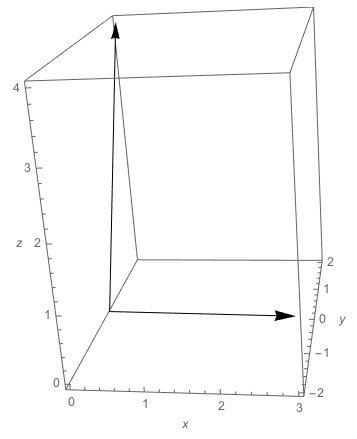
\includegraphics[scale=0.5]{figures_mvc/orthog_vecz}
	\end{center}
	\caption{Orthogonal vectors $\mathbf{u}=(3,-2,1)$ and $\mathbf{v}=(0,2,4)$.}
\end{figure}


We know from trigonometry that right angles are special, so it would be nice to have a way to check if two vectors written in component form are perpendicular. Fortunately, the dot product gives us an easy way to determine this. 
\begin{defn}[Orthogonal vectors]\label{prop:orthogonal_vectors}
	Two nonzero vectors ${\bf a}$ and ${\bf b}$ are said to be \emph{orthogonal} if ${\bf a}\cdot {\bf b}=0$.
\end{defn}
To see the significance of this definition, if ${\bf a}$ and ${\bf b}$ are non-zero then their dot product can be written as
\begin{align*}
	{\bf a}\cdot {\bf b}=||{\bf a}|| \ ||{\bf b}||\cos \theta.
\end{align*}	
Since $||{\bf a}||$ and $||{\bf b}||$ are both greater than zero, ${\bf a}\cdot {\bf b}=0$ if and only if $\theta=\frac{\pi}{2}$, that is, if and only if ${\bf a}$ and ${\bf b}$ are \emph{perpendicular}. Therefore for nonzero vectors being orthogonal (zero dot product) is the same as being perpendicular (intersecting at a right angle). Since $\mathbf{v}\cdot \mathbf{0}=0$ for every vector $\mathbf{v}$, the zero vector is orthogonal to every vector (including itself).

\begin{example}
The two vectors in the example above	
\begin{align*}
	{\bf u}&=(3,-2,1) \\
	{\bf v}&=(0,2,4).
\end{align*}
are orthogonal (and therefore indeed perpendicular) since ${\bf u}\cdot {\bf v}=3(0)-2(2)+1(4)=-4+4=0$.
\end{example}

\begin{defn}[Orthogonal set]
	A set of vectors $\{\mathbf{v}_1,\mathbf{v}_2,\dots,\mathbf{v}_n\}$ is said to be \emph{orthogonal} if $\mathbf{v}_i \cdot \mathbf{v}_j=0$ whenever $i \neq j$.
\end{defn}


\begin{example}
	The standard unit vectors for $\mathbb{R}^3$ form an orthogonal set. One can easily verify that 
	\begin{align*}
		{\bf e}_i \cdot {\bf e_j}=\delta_{ij}
	\end{align*}
where 
\begin{align*}
	\delta_{ij} \equiv \begin{cases}
		1 \text{ if } i=j, \\
		0 \text{ if } i \neq j
	\end{cases}
\end{align*}
is called the \ti{Kronecker delta symbol}. Since ${\bf e}_i \cdot {\bf e_j}=0$ whenever $i \neq j$, the set $\{e_1, e_2, e_3\}$ is indeed orthogonal. 
\end{example}
In the orthogonal set in the previous example, each vector in the set is a unit vector. Such a set has a special name:

\begin{defn}[Orthonormal set]
	An orthogonal set of vectors is said to be an \emph{orthonormal set} if each vector in the set is a unit vector.
\end{defn}


The examples above illustrate another difference between the dot product of two vectors and the ordinary product of two numbers. For two real numbers, if $ab=0$, then either $a=0$ or $b=0$. These examples clearly show that if ${\bf a}\cdot {\bf b}=0$, then it need not be true that either ${\bf a}=0$ or ${\bf b}=0$.
\subsubsection{Projection of a vector}
Let ${\bf a}$ be a nonzero vector, ${\bf \hat{a}}=\frac{{\bf a}}{||{\bf a}||}$ the unit vector obtained by normalizing ${\bf a}$, and ${\bf b}$ another vector. Then Eq. \eqref{eq:dot_product_def} shows that
\begin{align*}
	{\bf \hat{a}}\cdot {\bf b}=\frac{{\bf a}}{||{\bf a}||} \cdot {\bf b}=||{\bf b}||\cos \theta
\end{align*} 
is the component of ${\bf b}$ in the direction of ${\bf a}$. Multiplying by ${\bf \hat{a}}$, we get a vector parallel to ${\bf a}$ whose magnitude is the component of ${\bf b}$ along ${\bf a}$.

\begin{defn}[Vector projection]
	The vector $\text{proj}_{\bf a}{\bf b}\equiv ({\bf \hat{a}}\cdot {\bf b}){\bf \hat{a}}=||{\bf b}||\cos \theta {\bf \hat{a}}$ is called the \ti{projection of ${\bf b}$ onto ${\bf a}$}.
\end{defn}
Geometrically, the projection of ${\bf b}=\overrightarrow{PQ}$ onto ${\bf a}=\overrightarrow{PS}$ is the vector $\overrightarrow{PR}$ determined by connecting a perpendicular segment from $Q$ to the line $PS$. \footnote{Note that by using the definitions of the dot product and the norm of ${\bf a}$, one may produce many equivalent expressions for $\text{proj}_{\bf a}{\bf b}$:
\begin{align*}
	\text{proj}_{\bf a}{\bf b}&=(||{\bf b}||\cos \theta){\bf \hat{a}} \\
	&=({\bf \hat{a}}\cdot {\bf b}){\bf \hat{a}} \\
	&=\left(\frac{{\bf a}\cdot {\bf b}}{||{\bf a}||}\right)\frac{{\bf a}}{||{\bf a}||} \\
	&=\left(\frac{{\bf b}\cdot {\bf a}}{{\bf a}\cdot {\bf a}}\right){\bf a}
\end{align*}
The first of these is perhaps the easiest to remember, as it makes most transparent the relation to elementary right triangle trigonometry.}

\begin{center}
	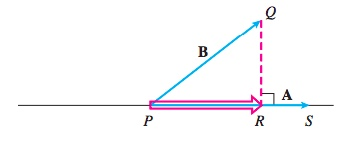
\includegraphics[scale=0.5]{figures_mvc/vector_projection_def}
\end{center}
Physically, if ${\bf b}$ represents a force, then $\text{proj}_{\bf a}{\bf b}$ is the 	``effective" force in the ${\bf a}$ direction; that is, the component of the force along ${\bf a}$.

\begin{center}
	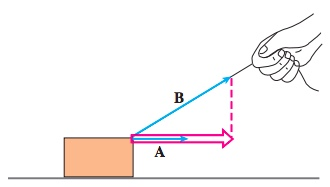
\includegraphics[scale=0.5]{figures_mvc/effective_force_box}
\end{center}	

It is often desirable to express a vector ${\bf b}$ as a sum of two orthogonal vectors. For instance, in mechanics we frequently decompose forces in this way so that we may treat a two-dimensional problem as two one-dimensional problems. We can easily express a vector ${\bf b}$ as such a sum of two vectors, one parallel to some nonzero vector ${\bf a}$ and one orthogonal to ${\bf a}$, in terms of the projection of ${\bf b}$ along ${\bf a}$:
\begin{equation}
\begin{split}
	{\bf b}&={\bf b}_{\parallel}+{\bf b}_{\perp} \\
	&=\text{proj}_{\bf a}{\bf b}+({\bf b}-\text{proj}_{\bf a}{\bf b}).
\end{split}
\end{equation}

\begin{center}
	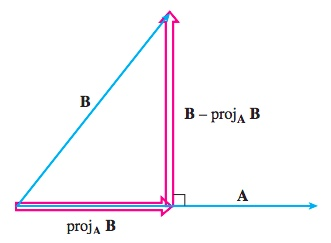
\includegraphics[scale=0.5]{figures_mvc/sum_of_orthogonal_vectors}
\end{center}

\begin{example}
	Express ${\bf b}=2{\bf e}_1+{\bf e}_2-3{\bf e}_3$ as the sum of a vector parallel to ${\bf a}=3{\bf e}_1-{\bf e}_2$ and a vector orthogonal to ${\bf a}$.
\end{example}

{\color{red} \flushleft {\bf Solution:}
Since ${\bf \hat{a}}\equiv \frac{{\bf a}}{||{\bf a}||}=\frac{3{\bf e}_1-{\bf e}_2}{\sqrt{10}}$, we can write ${\bf b}={\bf b}_{\parallel}+{\bf b}_{\perp}$ with  
\begin{align*}
	{\bf b}_{\parallel}&=({\bf \hat{a}}\cdot {\bf b}){\bf {\hat{a}}}=\frac{1}{2}(3{\bf e}_1-{\bf e}_2)=\frac{1}{2}{\bf a} \\
	{\bf b}_{\perp}&={\bf b}-{\bf b}_{\parallel}=\frac{1}{2}{\bf e}_1+\frac{3}{2}{\bf e}_2-3{\bf e}_3.
\end{align*}}

\subsection{Equations of lines and planes}
\subsubsection{Lines in space}
The coordinate systems of analytic geometry allow us to consider geometric objects such as lines and planes in terms of vectors. These geometric ideas will give us valuable intuition later on in the course when we take a more abstract point of view toward vectors.

First let us recall that any two points define a line. Equivalently, we can also determine a line if we know one point on the line and the slope of the line. 

Let us now work in Cartesian coordinates. Suppose $L$ is a line passing through a point $P_0(x_0,y_0,z_0)$ and parallel to a vector ${\bf v}=v_1{\bf e}_1+v_2{\bf e}_2+v_3{\bf e}_3$. Now let $P(x,y,z)$ be any point in space. In which case will $P(x,y,z)$ to be on the line? This will be the case if and only if the vector $\overrightarrow{P_0P}$ is parallel to ${\bf v}$, that is, if $\overrightarrow{P_0P}$ is a scalar multiple of ${\bf v}$. Therefore,
\begin{defn}[Vector equation for a line]
	The line through $P_0(x_0,y_0,z_0)$ and parallel of ${\bf v}$ is the set of all points $P(x,y,z)$ such that $\overrightarrow{P_0P}=t{\bf v}$, with $-\infty < t < \infty$. This equation is called the \ti{vector equation} of the line.
\end{defn}
In terms of Cartesian coordinates, the vector equation for the line becomes
\begin{align*}
	(x-x_0){\bf e}_1+(y-y_0){\bf e}_2+(z-z_0){\bf e}_3&=t(v_1{\bf e}_1+v_2{\bf e}_2+v_3{\bf e}_3) \\
	&=tv_1{\bf e}_1+tv_2{\bf e}_2+tv_3{\bf e}_3
\end{align*}
which implies
\begin{align*}
	(x-x_0-tv_1){\bf e}_1+(y-y_0-tv_2){\bf e}_2+(z-z_0-tv_3){\bf e}_3={\bf 0}
\end{align*}
and hence
\begin{equation}\label{eq:parametric_equations_line}
	x=x_0+tv_1, \hspace{0.25cm} y=y_0+tv_2, \hspace{0.25cm} z=z_0+tv_3.
\end{equation}
Thus, the vector equation of the line is equivalent to the three scalar equations in Eq. \eqref{eq:parametric_equations_line}, each of which is the usual equation for a line with slope $v_i$ in one variable $t$.

\begin{defn}[Parametric equations for a line]
	The standard parametrization of the line through $P_0(x_0,y_0,z_0)$ and parallel to ${\bf v}=v_1{\bf e}_1+v_2{\bf e}_2+v_3{\bf e}_3$ is given by
	\begin{align*}
		x=x_0+tv_1, \hspace{0.25cm} y=y_0+tv_2, \hspace{0.25cm} z=z_0+tv_3.
	\end{align*}
	These equations are called the (standard) \ti{parametric equations} for the line.
\end{defn}

\begin{example}
Find the parametric equations for the line through $(-2,0,4)$ and parallel to ${\bf v}=2{\bf e}_1+4{\bf e}_2-2{\bf e}_3$.	
\end{example}

{\color{red} \flushleft {\bf Solution:}
Plugging into Eq. \eqref{eq:parametric_equations_line} gives
\begin{align*}
	x=-2+2t, \hspace{0.25cm} y=4t, \hspace{0.25cm} z=4-2t.
\end{align*}}
\begin{center}
	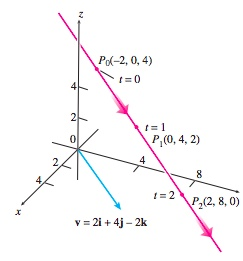
\includegraphics[scale=0.5]{figures_mvc/parametrized_line_example_1}
\end{center}

\begin{example}
	Find parametric equations for the line through $P(-3,2,-3)$ and $Q(1,-1,4)$.
\end{example}

{\color{red} \flushleft {\bf Solution:}
The vector from $P$ to $Q$ is 
\begin{align*}
	\overrightarrow{PQ}&=(1-(-3), -1-2, 4-(-3)) \\
	&=(4,-3,7).
\end{align*}
We take this vector to be our ``${\bf v}$". The point $P_0$ could be either $P$ or $Q$. Arbitrarily choosing it to be $Q$, Eq. \eqref{eq:parametric_equations_line} gives
\begin{align*}
	x=1+4t, \hspace{0.25cm} y=-1-3t, \hspace{0.25cm} z=4+7t.
\end{align*}}

\begin{example}
Parametrize the line segment joining the points $P(-3,2,-3)$ and $Q(1,-1,4)$.	
\end{example}
{\color{red} \flushleft {\bf Solution:}
We have seen in the previous exercise that the  parametric equations 
\begin{align*}
	x=1+4t, \hspace{0.25cm} y=-1-3t, \hspace{0.25cm} z=4+7t.
\end{align*}
describe an infinite line containing $P$ and $Q$ when we take $-\infty < t < \infty$. To describe the line segment joining $P$ and $Q$, we simply restrict the domain of $t$. We see that the line passes through $P$ at $t=-1$ and $Q=0$. So the line segment joining $P$ and $Q$ is given by 

\begin{align*}
	x=1+4t, \hspace{0.25cm} y=-1-3t, \hspace{0.25cm} z=4+7t.
\end{align*}

with $-1 < t < 0$.}

In $\mathbb{R}^2$, there is a unique normal direction to a given line. Let $\mathbf{n}=(n_1,n_2)$ be a normal vector to a line in $\mathbb{R}^2$ and $P_0(x_0,y_0)$ any point on the line (see Fig. \ref{fig:point_normal_eq_for_line} below). If $Q(x,y)$ is any other point on the line, then we must have
\begin{align*}
	\overrightarrow{P_0Q}\cdot \mathbf{n}=0.
\end{align*}
Since $\overrightarrow{P_0Q}=(x-x_0,y-y_0)$, 
\begin{align*}
	\overrightarrow{P_0Q}\cdot \mathbf{n}&=n_1(x-x_0)+n_2(y-y_0)=0
\end{align*}
or
\begin{align}\label{eq:point_normal_equation_for_line}
	n_1x+n_2y=c
\end{align}
where $c=n_1x_0+n_2y_0$. Equation \eqref{eq:point_normal_equation_for_line} is called the \emph{point normal} equation of the line.

\begin{figure}[h]\label{fig:point_normal_eq_for_line}
	\begin{center}
		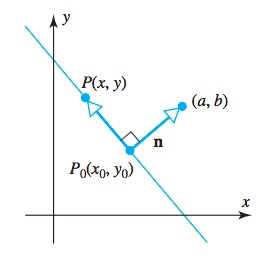
\includegraphics[scale=0.5]{figures_mvc/point_normal_eq_for_line}
	\end{center}
	\caption{Vectors involved in point normal equation of line.}
\end{figure}

\begin{example}
In $\mathbb{R}^2$ the equation
\begin{align*}
	6(x-3)+(y+7)=0
\end{align*}	
represents a line through the point $(3,-7)$ with normal vector $\mathbf{n}=(6,1)$.
\end{example}


\subsubsection{Planes in space}
Similar to a line in $\mathbf{R}^2$, a plane in $\mathbb{R}^3$ has a unique normal direction. We will now derive a point normal equation for a given plane. Let $\mathbf{n}=(n_1,n_2,n_3)$ be a normal vector to the plane. Given a point $P_0(x_0,y_0,z_0)$ on the plane and a vector ${\bf n}$ normal to the plane, what is the condition for an arbitrary point in space $P(x,y,z)$ to lie on the plane? If $P$ lies in the plane, the $\overrightarrow{P_0P}$ is a vector lying in the plane (see Fig. \ref{vector_equation_of_a_plane} below). Then, since ${\bf n}$ is normal to the plane, we must have that ${\bf n} \cdot \overrightarrow{P_0P}=0$.

\begin{figure}[h]\label{fig:vector_equation_of_a_plane}
	\begin{center}
	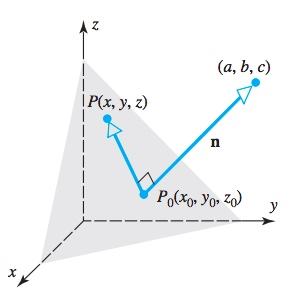
\includegraphics[scale=0.5]{figures_mvc/vector_equation_of_a_plane}
\end{center}
\caption{Vectors involved in point normal equation of plane.}
\end{figure}
Expanding the dot product in terms of components of these vectors, we obtain
	\begin{equation}
		n_1(x-x_0)+n_2(y-y_0)+n_3(z-z_0)=0.
	\end{equation}
or 
	\begin{equation}
		n_1x+n_2y+n_3z=c
	\end{equation}
	where $c=n_1x_0+n_2y_0+n_3z_0$. This is the \emph{point normal} equation of the plane.


\begin{example}
Find an equation for the plane through $P_0(-3,0,7)$ perpendicular to ${\bf n}=(5,2,-1)$.	
\end{example}

{\color{red} \flushleft {\bf Solution:}
The component equation is 
\begin{align*}
	5(x-(-3))+2(y-0)+(-1)(z-7)=0,
\end{align*}
Simplifying, we obtain
\begin{align*}
	5x+15+2y-z+7&=0 \\
	5x+2y-z&=-22.
\end{align*}}

\begin{example}
Find the point where the line 
\begin{align*}
	x=\frac{8}{3}+2t, \hspace{0.25cm} y=2t, \hspace{0.25cm} z=1+t
\end{align*}	
intersects the plane $3x+2y+6z=6$.
\end{example}

{\color{red} \flushleft {\bf Solution:}
The point $(\frac{8}{3}+2t, 2t, 1+t)$ lies in the plane if its coordinates satisfy the equation of the plane; that is, if
\begin{align*}
	3(\frac{8}{3}+2t)+2(-2t)+6(1+t)=6
\end{align*}
This has a solution at $t=-1$, so the point of intersection is 
\begin{align*}
	(x,y,z)\vert_{t=-1}=(\frac{2}{3},2,0).
\end{align*}}

\begin{exercise}
\begin{enumerate}[(a)]
	\item Find a vector parallel to the line of intersection of the planes $3x-6y-2z=15$ and $2x+y-2z=5$.	
	\item Find parametric equations for the line in which these planes intersect.
\end{enumerate}
\end{exercise}

\subsection{Some useful distance formulas}
\begin{thm}[Distance from point to line or plane] \hspace{15cm}
	\begin{enumerate}[(a)]
		\item In $\R^2$, the distance $D$ between the point $P_0(x_0,y_0)$ and the line $ax+by+c=0$ is 
		\begin{align}\label{eq:line_dist_formula}
			D=\frac{|ax_0+by_0+c|}{\sqrt{a^2+b^2}}
		\end{align}
		\item In $\R^3$ the distance $D$ between the point $P_0(x_0,y_0,z_0)$ and the plane $ax+by+cz+d=0$ is 
		\begin{align}\label{eq:plane_dist_formula}
			D=\frac{|ax_0+by_0+cz_0+d|}{\sqrt{a^2+b^2+c^2}}.
		\end{align}
	\end{enumerate}
\end{thm}

\begin{proof} \hspace{15cm}
	\begin{enumerate}[(a)]
		\item Left as an exercise. The steps are virtually identical to the proof in part (b).		
		\item Let $Q(x_1,y_1,z_1)$ be any point in the plane. Translate the normal vector $\mathbf{n}=(a,b,c)$ so that its initial point is at $Q$. 
	\begin{figure}[h]
		\begin{center}
			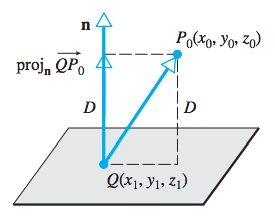
\includegraphics[scale=0.5]{figures_mvc/dist_to_plane_book}
		\end{center}
		\caption{Distance from $P_0$ to the plane.}
	\end{figure} 
		
		The distance $D$ is then the length of the projection $\text{proj}_{\mathbf{n}}\overrightarrow{QP_0}$:
		\begin{align*}
			D&=||\text{proj}_{\mathbf{n}}\overrightarrow{QP_0}|| \\
			&=\left|\left|\frac{\overrightarrow{QP_0}\cdot \mathbf{n}}{\mathbf{n}\cdot \mathbf{n}}\mathbf{n} \right|\right| \\
			&=\left|\frac{\overrightarrow{QP_0}\cdot \mathbf{n}}{\mathbf{n}\cdot \mathbf{n}}\right|||\mathbf{n}|| \\
			&=\frac{|\overrightarrow{QP_0}\cdot \mathbf{n}|}{||\mathbf{n}||^2}||\mathbf{n}|| \\
			&=\frac{|\overrightarrow{QP_0}\cdot \mathbf{n}|}{||\mathbf{n}||}
		\end{align*}
		Now
		\begin{align*}
			\overrightarrow{QP_0}&=(x_0-x_1,y_0-y_1,z_0-z_1), \\
			\overrightarrow{QP_0}\cdot{n}&=a(x_0-x_1)+b(y_0-y_1)+c(z_0-z_1), \\
			||\mathbf{n}||&=\sqrt{a^2+b^2+c^2}.
		\end{align*}
		and therefore
	\begin{align}\label{eq:dist_p_0_to_plane}
			D&=\frac{|\overrightarrow{QP_0}\cdot \mathbf{n}|}{||\mathbf{n}||}\\
			&=\frac{|a(x_0-x_1)+b(y_0-y_1)+c(z_0-z_1)|}{\sqrt{a^2+b^2}}.
		\end{align}
		Since the point $Q(x_1,y_1,z_1)$ lies in the plane, its coordinates satisfy the equation of the plane; thus
		\begin{align*}
			ax_1+by_1+cz_1+d=0
		\end{align*}
		or 
		\begin{align*}
			d=-ax_1-by_1-cz_1.
		\end{align*}
		Substituting this expression into \eqref{eq:dist_p_0_to_plane} yields \eqref{eq:plane_dist_formula}.
	\end{enumerate}
\end{proof}

\begin{example}
By \eqref{eq:plane_dist_formula}, the distance $D$ between the point $P_0(1,-4,-3)$ and the plane $2x-3y+6z=-1$ is
\begin{align*}
	D=\frac{|2(1)+(-3)(-4)+6(-3)+1|}{\sqrt{2^2+(-3)^2+6^2}}=\frac{|-3|}{7}=\frac{3}{7}.
\end{align*}	
\end{example}

The formula \eqref{eq:dist_p_0_to_plane} also allows us to compute the distance between parallel planes.

\begin{example}
The planes
\begin{align*}
	x+2y-2z=3 \hspace{0.25cm} \text{ and } \hspace{0.25cm} 2x+4y-4z=7
\end{align*}	
are parallel since their normal vectors $(1,2,-2)$ and $(2,4,-4)$ are parallel vectors. To find the distance $D$ between the planes, we just select an arbitrary point $P_0$ on one of the planes and then compute its distance to the other plane using \eqref{eq:dist_p_0_to_plane}. By setting $y=z=0$ in the equation $x+2y-2z=3$, we obtain the point $P_0(3,0,0)$ in this plane. The distance between $P_0$ and the plane $2x+4y-4z=7$ is then
\begin{align*}
	D=\frac{|2(3)+4(0)+(-4)(0)-7|}{\sqrt{2^2+4^2+(-4)^2}}=\frac{1}{6}.
\end{align*} 
\end{example}


\section{Systems of linear equations}
We will now change gears and turn to a seemingly distinct topic: that of finding solutions to systems of linear equations. However, we will quickly see that this task is intimately related to the vector operations we have just studied in the previous section.
\subsection{Basic definitions}
\begin{defn}[Linear equation]\label{def:linear_equation}
	A \ti{linear equation} in the variables $x_1,\cdots, x_n$ is an equation that can be written in the form
\begin{equation}
	a_1 x_1+a_2 x_2+\cdots a_n x_n=b
\end{equation}
where $b$ and the \emph{coefficients} $a_1,\cdots, a_n$ are real numbers.	
\end{defn}

\begin{exercise}
\bf Which of the following equations are linear?
\begin{enumerate}[(a)]
	\item $4x_1-5x_2+2=x_1$
	\item $x_2=2\sqrt{x_1}-6$
	\item $2x_1+x_2-x_3=2\sqrt{6}$ 
	\item $4x_1-5x_2=x_1x_2$ 
\end{enumerate}
\end{exercise}

\begin{defn}[System of linear equations]\label{eq:system_of_linear_equations}
	A \ti{system of linear equations} (or a \ti{linear system}) is a collection of one or more linear equations involving the \ti{same} variables $x_1, \cdots, x_n$.	
\end{defn}

\begin{example}
The following is a system of two linear equations in three variables $x_1,x_2,x_3$:
\begin{equation}\label{eq:system}
\begin{split}
	2x_1-x_2+1.5x_3&=8 \\
	x_1  \hspace{1.0cm} - \ 4x_3&=-7
\end{split}
\end{equation}	
\end{example}

\begin{defn}[Solution]\label{def:solution}
	Any $n$-tuple $(s_1,\cdots,s_n)$ of numbers which satisfies \ti{each} equation in a linear system when $s_1,\cdots,s_n$ are substituted for $x_1,\cdots,x_n$ is called a \ti{solution} of the system.
\end{defn}

\begin{example}[Testing a solution]
The 3-tuple $(5,6.5,3)$ is a solution of the system \eqref{eq:system} since
	\begin{equation*}
\begin{split}
	2(5)-6.5+1.5(3)&=8 \\
	5  \hspace{1.0cm} - \ 4(3)&=-7
\end{split}
\end{equation*}	
\end{example}

\begin{defn}[Solution set] \label{def:solution_set}
The set of all solutions is called the \ti{solution set} of the linear system.	
\end{defn}

\begin{defn}[Consistent and inconsistent systems]\label{def:consistent}
If a system of equations has at least one solution it is said to be \emph{consistent}. If the system has no solutions, it is said to be \emph{inconsistent}.	
\end{defn}

\begin{exercise}
Is $(3,4,-2)$ a solution of the following linear system?
\begin{align*}
	5x_1-x_2+2x_3 &=7 \\
	-2x_1+6x_2+9x_3&=0 \\
	-7x_1+5x_2-3x_3&=-7
\end{align*} 	
\end{exercise}

We have just seen how to check if a given point is a solution to a linear system. Obviously checking points at random is not going to be an effective strategy to find the solution set of a given linear system. We will therefore need a systematic method of finding solution sets of systems of linear equations. But first, let us consider what kind of solution sets we might hope to find.

\begin{example}[Two linear equations in two unknowns]\label{ex:two_linear_equations_in_two_unknowns}
Consider the most general linear system of two equations in two unknowns
\begin{equation}\label{eq:2_eq_2_var}
	\begin{split}
				A_{11} x_1+A_{12}x_2&=b_1, \\
		A_{21} x_1+A_{22}x_2&=b_2. 
	\end{split}
\end{equation}	
Rewriting each equation in slope-intercept form, \eqref{eq:2_eq_2_var} becomes
\begin{equation}
	\begin{split}
		x_2&=-\frac{A_{11}}{A_{12}}x_1+\frac{b_1}{A_{12}}, \\
		x_2&=-\frac{A_{21}}{A_{22}}x_1+\frac{b_2}{A_{22}}.
	\end{split}
\end{equation}
Geometrically, each equation describes a line in the plane. Since these equations are in the same variables, the two lines lie in the \emph{same} plane. A solution to the linear system corresponds to a point which lies on \emph{both} lines at the same time, i.e., it is a point of intersection of the two lines. It is geometrically evident that there are three possibilities for the possible solution sets of the linear system \eqref{eq:2_eq_2_var}, depending on the coefficients:
\begin{enumerate}[(1)]
	\item The linear system \eqref{eq:2_eq_2_var} has \emph{no solution} when 
	\begin{align*}
		\frac{A_{11}}{A_{12}}&=\frac{A_{21}}{A_{22}}, \\
		b_1 & \neq b_2,
	\end{align*}
i.e., when the lines are parallel (same slope) but non-overlapping (different y-intercepts).
\begin{center}
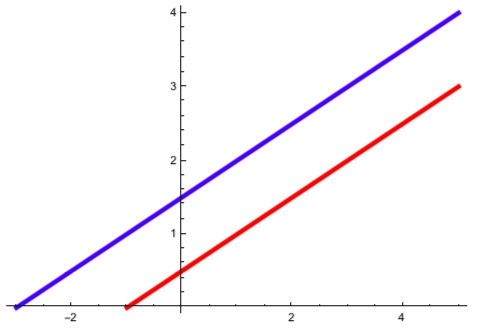
\includegraphics[scale=0.5]{figures_mvc/two_lines_no_soln}
\end{center}

\item The linear system \eqref{eq:2_eq_2_var} has \emph{infinitely many solutions} when 
	\begin{align*}
		\frac{A_{11}}{A_{12}}&=\frac{A_{21}}{A_{22}}, \\
		b_1 & = b_2,
	\end{align*}
	i.e., when the lines are overlapping (both described by exactly the same equation).
	\begin{center}
	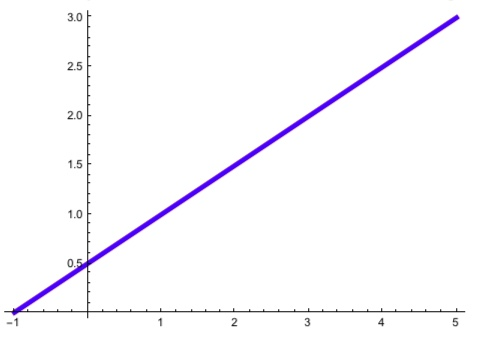
\includegraphics[scale=0.5]{figures_mvc/two_lines_inf_soln}		
	\end{center}

\item The linear system \eqref{eq:2_eq_2_var} has a \emph{unique solution} in all other cases (i.e., when the lines are non-parallel).
\begin{center}
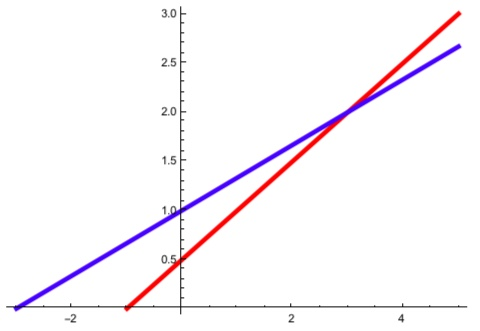
\includegraphics[scale=0.5]{figures_mvc/two_lines_unique_soln}	
\end{center}
\end{enumerate}
\end{example}

In general, we will consider a linear system of $m$ equations in $n$ unknowns:
\begin{equation}\label{eq:m_eq_n_var}
\begin{split}
	A_{11}x_1+A_{12}x_2+\cdots + A_{1n}x_n &=y_1 \\
	A_{21}x_1+A_{22}x_2+\cdots + A_{2n}x_n &=y_2 \\
	\vdots \hspace{1.5cm} \vdots \hspace{2.5cm} \vdots & \hspace{0.5cm}\vdots  \\
	A_{m1}x_1+A_{m2}x_2+\cdots + A_{mn}x_n &=y_m \\
\end{split}	
\end{equation}
where $y_1,\cdots, y_m$ and $A_{ij}, 1 \leq i \leq m, 1 \leq j \leq n$ are given. In \eqref{eq:m_eq_n_var}, we denote the coefficient of $x_j$ in the $i$th equation as $A_{ij}$.

As we will see \fixme{Insert link to proof.}, it turns out that the three possibilities in Example \ref{ex:two_linear_equations_in_two_unknowns} are the only possibilities in general; that is, the general linear system in \eqref{eq:m_eq_n_var} has either 
\begin{enumerate}
	\item No solution,
	\item A unique solution, or
	\item Infinitely many solutions.
\end{enumerate}
We can again understand this claim geometrically in the case of three linear equations in three unknowns:
\begin{align*}
	A_{11}x_1+A_{12}x_2+A_{13}x_3&=y_1 \\
	A_{21}x_1+A_{22}x_2+A_{23}x_3&=y_1 \\
	A_{31}x_1+A_{32}x_2+A_{33}x_3&=y_1.
\end{align*}
These are the point-normal equations of three planes in $\R^3$. The possible intersections are shown below, giving rise to the types of solution sets mentioned above:
\begin{figure}[h]
	\begin{center}
		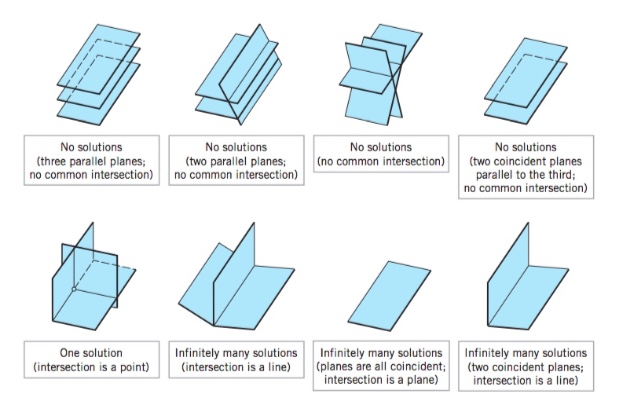
\includegraphics[scale=0.5]{figures_mvc/plane_intersections_anton_fig}
	\end{center}
	\caption{The intersections of three planes give the solution sets of a linear system of three equations in three unknowns.}
\end{figure}
\newpage 
\begin{exercise}
To get comfortable with the notation in \eqref{eq:m_eq_n_var}, write out the system \eqref{eq:m_eq_n_var} when 
\begin{enumerate}[(a)]
	\item $n=2,m=3$, 
	\item $m=3,n=2$, and 
	\item $m=n=3$. 
\end{enumerate}	
\end{exercise}



\begin{defn}[Homogeneous and inhomogeneous sytems]\label{def:homogeneous_and_inhomogeneous_sytems}
If $y_1=y_2=\cdots=y_m=0$ in 
\eqref{eq:2_eq_2_var}, the system is said to be \emph{homogeneous}. Otherwise, it is said to be \emph{inhomogeneous}.
\end{defn}

\begin{exercise}
	Write down a homogeneous system of $3$ linear equations in $2$ unknowns.
\end{exercise}

\subsection{Elimination}
A fundamental technique for finding the solutions of a system of linear equations is that of \emph{elimination} of variables. Roughly, this technique involves multiplying the equations in the system by numbers and then adding the resulting equations together so that some of the variables drop out, leading to a simpler system of equations.
\begin{example}[Solving by elimination]
To illustrate this technique, consider the homogeneous system
	\begin{align}\label{eq:ex_2_10_eq_1}
		2x_1-x_2+x_3&=0 \\ \label{eq:ex_2_10_eq_2}
		x_1+3x_2+4x_3&=0. 
	\end{align} 
Adding $(-2) \cdot $ \eqref{eq:ex_2_10_eq_2} $+$\ \eqref{eq:ex_2_10_eq_1}  gives $-7x_2-7x_3=0$ or 
\begin{equation}\label{eq:ex_2_10_cond_1}
	x_2=-x_3.
\end{equation}
Adding
$3$ \eqref{eq:ex_2_10_eq_1} $+$ \ \eqref{eq:ex_2_10_eq_2} gives $7x_1+7x_3=0$ or 
\begin{equation}\label{eq:ex_2_10_cond_2}
	x_1=-x_3.
\end{equation}

Thus, a solution of this system is obtained by setting $x_3=t$, where $t$ is any real number, and then solving for $x_1$ and $x_2$ in terms of $t$ using \eqref{eq:ex_2_10_cond_1} and \eqref{eq:ex_2_10_cond_2}. The solution set can therefore be written as $\{(-t,-t,t): t \in \mathbb{R}\}$, which is said to be written in \emph{parametric form}. We see that there is a solution for each $t \in \R$, so this system has an infinite number of solutions.
  \end{example}
 \begin{exercise}\label{ex:verify_is_indeed_solution}
 Verify that $(-t,-t,t)$ is indeed a solution of the system of equations in the previous example for any $t \in \R$.	
 \end{exercise}


We now begin to formalize the elimination process in order to carry it out in a systematic way and to understand why it works. Consider again the general linear system of $m$ equations in $n$ unknowns in \eqref{eq:m_eq_n_var}. If we select $m$ scalars $c_1,\cdots,c_m$, multiply the $j$th equation by $c_j$ for $j=1,\cdots,m$, and add all of the equations together, we obtain a new linear equation, given by \footnote{In this language, equations \eqref{eq:ex_2_10_cond_1} and \eqref{eq:ex_2_10_cond_2} in the previous example were obtained in exactly this way, as linear combinations of equations \eqref{eq:ex_2_10_eq_1} and \eqref{eq:ex_2_10_eq_2}.}
\begin{equation}\label{eq:linear_combination_of_equations}
	\begin{split}
		(c_1A_{11}+c_2A_{21}+\cdots+c_mA_{m1})x_1+\cdots+(&c_1A_{1n}+c_2A_{21}+\cdots+c_mA_{mn})x_n \\ &= c_1y_1+\cdots +c_m y_m.
	\end{split}
\end{equation}

\begin{defn}[Linear combination]\label{def:linear_combination_of_equations}
The equation \eqref{eq:linear_combination_of_equations} is said to be a \emph{linear combination} of the equations in \eqref{eq:m_eq_n_var}.
\end{defn}

\begin{thm}[Linear combinations of linear equations preserve solutions]\label{prop:linear_combinations_of_linear_equations_preserve_solutions}
If $(s_1,\cdots,s_n)$ is a solution of the linear system \eqref{eq:m_eq_n_var}, then it is also a solution of \eqref{eq:linear_combination_of_equations}.	
\end{thm}

\begin{pf}
	Substituting $(x_1,\cdots,x_n)=(s_1,\cdots,s_n)$ in \eqref{eq:linear_combination_of_equations} gives
\begin{align*}
	&(c_1A_{11}+c_2A_{21}+\cdots+c_mA_{m1})s_1+\cdots+(c_1A_{1n}+c_2A_{21}+\cdots+c_mA_{mn})s_n  \\
	&=c_1(A_{11}s_1+\cdots + A_{1n}s_n)+\cdots + c_m(A_{m1}s_1+\cdots + A_{mn}s_n) \\
	&= c_1y_1 + \cdots + c_my_m,
\end{align*}
where we have used the fact that $A_{i1}s_1+\cdots + A_{in}s_n=y_i$ for $i=1,\dots,m$, that is, that $(s_1,\dots,s_n)$ is a solution to the original system of equations. \footnote{This is exactly what you verified in Exercise \ref{ex:verify_is_indeed_solution}.}
\end{pf}

\emph{Theorem \ref{prop:linear_combinations_of_linear_equations_preserve_solutions} is the fundamental idea of the elimination process}: given the linear system \eqref{eq:m_eq_n_var}, if we have another linear system 
	\begin{equation}\label{eq:another_system}
\begin{split}
	B_{11}x_1+B_{12}x_2+\cdots + B_{1n}x_n &=z_1 \\
	B_{21}x_1+B_{22}x_2+\cdots + B_{2n}x_n &=z_2 \\
	\vdots \hspace{1.5cm} \vdots \hspace{2.5cm} \vdots & \hspace{0.5cm}\vdots  \\
	B_{k1}x_1+B_{k2}x_2+\cdots + B_{kn}x_n &=z_k \\
\end{split}
\end{equation}
in which each of the $k$ equations is a linear combination of the equations in \eqref{eq:m_eq_n_var}, then \emph{every solution of \eqref{eq:m_eq_n_var} is a solution of this new system}. 
Thus, \emph{the elimination process allows us to solve a linear system by forming linear combinations of the given equations to produce an system of equations which has the same solutions, but is easier to solve}. 

Of course, it may happen that some solutions of \eqref{eq:another_system} are not solutions of \eqref{eq:m_eq_n_var}. As a simple example, consider the following two linear systems:
\begin{align}
		x_1-2x_2&=-1 \label{eq:e1}\\
		-x_1+3x_2&=3 \label{eq:e2}
\end{align} 
and 
\begin{align}
		x_1-2x_2&=-1 \label{eq:e3}\\
		-x_1+2x_2&=1 \label{eq:e4}
\end{align}
Using the elimination technique, the former system has a unique solution $(3,2)$ whereas the latter has an infinite number of solutions, which we can parametrize as $\{(2t-1,t):t \in \mathbb{R}\}$. By taking $t=2$, we see that $(3,2)$ is a solution of the second system, but any solution of the second system with $t \neq 2$ is not a solution of the first.

This can be understood as follows: Both equations in the second system can be written as linear combinations of the equations in the first system, since 
\begin{align*}
	\eqref{eq:e3}&=1\cdot \eqref{eq:e1}+0\cdot \eqref{eq:e2} \\
	\eqref{eq:e4}&=-1\cdot \eqref{eq:e1}+0\cdot \eqref{eq:e2}
\end{align*}
However, the second equation in the first system  cannot be written as a linear combination of the equations in the second system.

\begin{exercise}
Show that 
\begin{align*}
	c_1 \eqref{eq:e3} + c_2 \eqref{eq:e4} = \eqref{eq:e2}
\end{align*}
requires 
\begin{align*}
	c_1-c_2&=-1 \\
	c_1-c_2&=-3,
\end{align*}	
which has no solution.
\end{exercise}

This motivates the following definition:

\begin{defn}[Equivalent linear systems] \label{def: equivalent_linear_systems}
	Two systems of linear equations are said to be \emph{equivalent} if they have the same set of solutions.
\end{defn}

We have just seen that two linear systems might fail to be equivalent if the equations in one system cannot be written as linear combinations of the equations in the other system. We thus have the following theorem:

\begin{thm}[Equivalent linear systems]\label{prop:equivalent_linear_systems}
	Two systems of linear equations are equivalent if each equation in each system is a linear combination of the equations in the other system. 
\end{thm}

\begin{pf}
	The proof follows immediately from Theorem \ref{prop:linear_combinations_of_linear_equations_preserve_solutions}.
\end{pf}

\begin{exercise}
Are the following two systems of linear equations equivalent? If so, express each equation in each system as a linear combination of the equations in the other system.
\begin{align*}
	 x_1-x_2=0 \hspace{1.0cm} 3x_1+x_2&=0 \\
	2x_1+x_2=0 \hspace{1.0cm} x_1+x_2&=0
\end{align*}	
\end{exercise}

If the elimination process is to be effective in finding the solutions of the system \eqref{eq:m_eq_n_var}, then we must see how to form linear combinations of the given equations to produce an equivalent system of equations which is easier to solve. In the next section, we discuss a method to systematically do this. We begin by developing a more convenient notation.

\subsection{Matrices}
Given the general system of $m$ linear equations in $n$ unknowns in \eqref{eq:m_eq_n_var}, we wish to form linear combinations of these equations in such a way that we are guaranteed to produce an equivalent system which is easier to solve. In this section, we will formalize this process and make precise the kind of system at which we wish to arrive.

	In forming linear combinations of the equations in \eqref{eq:m_eq_n_var}, notice that we are actually only computing with the coefficients $A_{ij}$ and scalars $y_i$, with the variables $x_j$ more or less acting as placeholders. We shall therefore abbreviate the system by
	\begin{equation}
		AX=Y
	\end{equation}
	where 
	\begin{equation}\label{eq:coeff_matrix}
		A=\begin{bmatrix}
			A_{11} \cdots A_{1n} \\
			\vdots \hspace{1.3cm} \vdots \\
			A_{m1} \cdots A_{mn}
		\end{bmatrix}
	\end{equation} 
	\begin{equation}
		X=\begin{bmatrix}
			x_1 \\ \vdots \\ x_n
		\end{bmatrix} \ \text{ and } Y= \begin{bmatrix}
			y_1 \\ \vdots \\ y_m
		\end{bmatrix}
	\end{equation} 
\begin{defn}[Coefficient matrix] \label{def:coefficient_matrix}
	A rectangular array of numbers as in \eqref{eq:coeff_matrix} is called a \ti{matrix}. In \eqref{eq:coeff_matrix}, the matrix $A$ is called the \ti{coefficient matrix} of the system. The $mn$ numbers $A_{ij}$ (which are the coefficients of the equations in \eqref{eq:m_eq_n_var}) are called the \ti{entries} (or \ti{matrix elements}) of the matrix $A$. Since $A$ has $m$ rows and $n$ columns, it is said to be an $m \times n$ matrix. Note that the number of \emph{rows} is always listed first. \footnote{For now $AX=Y$ is simply a shorthand notation for the system \eqref{eq:m_eq_n_var}.
	We will soon define a multiplication operation for matrices such that the product of $A$ and $X$ is $Y$.}
\end{defn}

\begin{example}[Coefficient matrix of a linear system]
	The matrix of coefficients for the linear system
		\begin{align*}
		2x_1-x_2+x_3&=0 \\
		x_1+3x_2+4x_3&=0
	\end{align*} 
is
\begin{align*}
	A=\begin{bmatrix}
		2&-1&1 \\ 1&3&4
	\end{bmatrix}.
\end{align*}	
\end{example}

\begin{exercise}
	Write the coefficient matrix for the linear system
\begin{align*}
		x_1-2x_2+x_3&=0 \\
		2x_2-8x_3 &=0 \\
		5x_1-5x_3 &=0.
	\end{align*}
\end{exercise}

\subsection{Elementary row operations}
We now consider operations on the rows of the matrix $A$ which correspond to forming linear combinations of the equations in the system $AX=Y$. 
	We only wish to consider operations which lead to an \ti{equivalent} system of equations.
	As we will see, any such operation can built out of three \ti{elementary row operations}:
\begin{defn}[Elementary row operations] \label{def:elementary_row_operations}
The three \ti{elementary row operations} are the following:
\begin{enumerate}
	\item (Replacement) Replace one row by the sum of itself and a multiple of another row.
	\item (Interchange) Interchange two rows.
	\item (Scaling) Multiply all entries in a row by a \emph{nonzero} constant.
\end{enumerate}	
\end{defn}

More formally, we can view each elementary row operation as a \emph{function} $e$ which takes an $m \times n$ matrix $A$ to an $m \times n$ matrix $e(A)$. The function is specified on the matrix elements $A_{ij}$ of $A$ explicitly in each of the three cases above as follows:

\begin{enumerate}
	\item $e(A)_{ij}=\begin{cases}
		A_{ij} \text{ if } i \neq r, \\
		A_{rj}+c A_{sj} \text{ if } i = r.
	\end{cases}$
	\item $e(A)_{ij}=\begin{cases}
		A_{ij} \text{ if } i \neq r,s, \\
		A_{sj} \text{ if } i = r, \\
		A_{rj} \text{ if } i=s.
	\end{cases}$
	\item $e(A)_{ij}=\begin{cases}
		A_{ij} \text{ if } i \neq r, \\
		cA_{rj} \text{ if } i = r.
	\end{cases}$
\end{enumerate}

One reason we restrict to these three elementary row operations is that they each have an inverse (which is itself an elementary row operation of the same type), allowing us to recover the original matrix $A$ from $e(A)$. This is crucial in making sure the resulting linear system is equivalent to the original one.

\begin{exercise}
For each pair of matrices below, find the elementary row operation that transforms the first matrix into the second, and then find the inverse row operation that transforms the second matrix into the first.
	\begin{enumerate}
		\item $\begin{bmatrix}
			0&-2&5 \\ 1&4&-7 \\ 3&-1&6
		\end{bmatrix}, \begin{bmatrix}
			1&4&-7 \\ 0&-2&5 \\ 3&-1&6
		\end{bmatrix}$
		\item $\begin{bmatrix}
			1&3&-4 \\ 0&-2&6 \\ 0&-5&9
		\end{bmatrix}, \begin{bmatrix}
			1&3&-4 \\ 0&1&-3 \\ 0&-5&9
		\end{bmatrix}$
		\item $\begin{bmatrix}
			1&-2&1&0 \\ 0&5&-2&8 \\ 4&-1&3&-6
		\end{bmatrix}, \begin{bmatrix}
			1&-2&1&0 \\0&5&-2&8 \\ 0&7&-1&-6
		\end{bmatrix}$
		\item $\begin{bmatrix}
			1&2&-5&0 \\ 0&1&-3&-2 \\ 0&-3&9&5
		\end{bmatrix}, \begin{bmatrix}
			1&2&-5&0 \\ 0&1&-3&-2 \\ 0&0&0&-1
		\end{bmatrix}$
	\end{enumerate}	
\end{exercise}


\begin{thm}[Elementary row operations are invertible]\label{thm:elementary_row_operations_are_invertible}
	To each elementary row operation $e$ there corresponds an elementary row operation $e^{-1}$ of the \emph{same} type as $e$, such that $e^{-1}(e(A))=e(e^{-1}(A))=A$ for all $A$.
\end{thm}

\begin{pf} We consider each type of elementary row operation in turn. 
\begin{enumerate}[(1)]
	\item If $e$ is the operation which replaces row $r$ by row $r$ plus $c$ times row $s$ ($r \neq s$), then $e^{-1}$ is the operation which replaces row $r$ by row $r$ plus $(-c)$ times row $s$. To see this, note that composing these operations leaves $A_{ij}$ unchanged if $i\neq r$ and sends $A_{rj} \mapsto A_{rj}+cA_{sj} \mapsto (A_{rj}+cA_{sj})-cA_{sj}=A_{rj}$.
	\item If $e$ interchanges rows $r$ and $s$, then $e^{-1}=e$.
	\item If $e$ be the operation which multiplies the $r$th row of a matrix by the non-zero scalar $c$, then $e^{-1}$ is the operation which multiplies the $r$th row by $\frac{1}{c}$, since composing these operations sends $A_{rj} \mapsto cA_{rj} \mapsto \frac{1}{c}(cA_{rj})=A_{rj}$ and leaves $A_{ij}$ unchanged if $i \neq r$. 
\end{enumerate}
\end{pf}

\begin{defn}[Row-equivalent matrices]\label{def:row_equivalent_matrices}
	Two $m \times n$ matrices are said to be \ti{row-equivalent} if one can be obtained from the other by a finite sequence of elementary row operations. 
\end{defn}

\begin{lem}[Row-equivalence is an equivalence relation]\label{lem:row_equivalence_is_an_equivalence_relation}
Row-equivalence is an equivalence relation. That is, if $A,B$ and $C$ are any $m \times n$ matrices, then they satisfy the following properties
\begin{enumerate}[(i)]
	\item (Relfexivity) $A$ is row-equivalent to itself;
	\item (Symmetry) If $A$ is row-equivalent to $B$, then $B$ is row-equivalent to $A$;
	\item (Transitivity) If $A$ is row-equivalent to $B$, and $B$ is row-equivalent to $C$, then $A$ is row-equivalent to $C$.
\end{enumerate}
\end{lem}
\begin{pf}
\begin{enumerate}[(i)]
	\item (Reflexivity) $A$ is equal to itself by an empty sequence of elementary row operations, hence $A$ is row-equivalent to itself. 
	\item (Symmetry) If $A$ is row-equivalent to $B$, then $B=(e_n \circ e_{n-1} \circ \cdots e_1)(A)$. Then $A=(e_1^{-1}\circ \cdots \circ e_{n-1}^{-1} \circ e_n^{-1})(B)$ (since $e_j^{-1}(e_j(A))=A$ and $e_j(e_j^{-1}(B))=B$ for all $j=1,\dots,n$), hence $B$ is row-equivalent to $A$. 
	\item (Transitivity) If $A$ is row-equivalent to $B$ and $B$ is row-equivalent to $C$, then $B=(e_n \circ \cdots \circ e_1)(A)$ and $C=(\tilde{e}_m \circ \cdots \circ \tilde{e}_1)(B)$. We therefore have $C=(\tilde{e}_m \circ \cdots \circ \tilde{e}_1\circ e_n \cdots \circ e_1)(A)$, hence $A$ is row-equivalent to $C$.
\end{enumerate}	
\end{pf}

\begin{thm}[Row-equivalence implies equivalence]\label{thm:row_equivalence_implies_equivalence}
	If $A$ and $B$ are row-equivalent $m \times n$ matrices, then the linear systems $AX=0$ and $BX=0$ are equivalent (have exactly the same solutions).	
\end{thm}

\begin{pf}
	Since we pass from $A$ to $B$ by a finite sequence of elementary row operations
$$A=A_0 \to A_1 \to \cdots \to A_k=B,$$
by transitivity (see Lemma \ref{lem:row_equivalence_is_an_equivalence_relation}) it suffices to prove that the systems $A_jX=0$ and $A_{j+1}X=0$ have the same solutions, i.e., that one elementary row operation does not disturb the set of solutions. 

 Suppose now that $B$ is obtained from $A$ by a single elementary row operation. For each of the three types of elementary row operations, each equation in the system $BX=0$ will be a linear combination of the equations in the system $AX=0$. Since the inverse of an elementary row operation is an elementary row operation, each equation in $AX=0$ will also be a linear combination of the equations in $BX=0$. Hence, these two systems are equivalent.
\end{pf}

\begin{example}[Solving a homogeneous system of equations by elementary row operations] We now demonstrate how to use 
	Theorem \ref{thm:row_equivalence_implies_equivalence} to solve a homogeneous system of liner equations by elementary row operations. 
	
	Consider the homogeneous system of linear equations
	\begin{equation}\label{eq:hom_ex_original}
	\begin{split}
2x_1-x_2+3x_3+2x_4 &=0 \\
x_1+4x_2-x_4&=0 \\
2x_1+6x_2-x_3+5x_4 &=0.
	\end{split}
	\end{equation}
We write the coefficient matrix of the system and apply the following sequence of elementary row operations:
\begin{align*}
	&\begin{bmatrix}
		2&-1&3&2 \\ 1 & 4 & 0 & -1 \\2 & 6 & -1 & 5
	\end{bmatrix} \stackrel{\footnotesize{R3 \to -R1+R3}}{\longrightarrow}	\begin{bmatrix}
		2&-1&3&2 \\ 1 & 4 & 0 & -1 \\0&7&-4&3
	\end{bmatrix}\stackrel{\footnotesize{R1 \to \frac{1}{2}R1}}{\longrightarrow} \\
	&\begin{bmatrix}
		1&-1/2&3/2&1 \\ 1 & 4 & 0 & -1 \\0&7&-4&3
	\end{bmatrix}\stackrel{\footnotesize{R2 \to -R1+R2}}{\longrightarrow} \begin{bmatrix}
		1&-1/2&3/2&1 \\ 0 & 9/2 & -3/2 & -2 \\0&7&-4&3
	\end{bmatrix} \stackrel{\footnotesize{R2 \to \frac{2}{9}R2}}{\longrightarrow} \\
	&{\footnotesize\begin{bmatrix}
		1&-1/2&3/2&1 \\ 0 & 1 & -1/3 & -4/9 \\0&7&-4&3
	\end{bmatrix}} \stackrel{\footnotesize{R3 \to -7R2+R3}}{\longrightarrow} {\footnotesize \begin{bmatrix}
		1&-1/2&3/2&1 \\ 0 & 1 & -1/3 & -4/9 \\0&0&-5/3&55/9
	\end{bmatrix} }\stackrel{\footnotesize{R3 \to -\frac{3}{5}R3}}{\longrightarrow} \\
	&\begin{bmatrix}
		1&-1/2&3/2&1 \\ 0 & 1 & -1/3 & -4/9 \\0&0&1&-11/3
	\end{bmatrix} \stackrel{\footnotesize{R2 \to \frac{1}{3}R3+R2}}{\longrightarrow}\begin{bmatrix}
		1&-1/2&3/2&1 \\ 0 & 1 & 0 & -5/3 \\0&0&1&-11/3
	\end{bmatrix}\stackrel{\footnotesize{R1 \to -\frac{3}{2}R3+R1}}{\longrightarrow}\\
	&\begin{bmatrix}
		1&-1/2&0&13/2 \\ 0 & 1 & 0 & -5/3 \\0&0&1&-11/3
	\end{bmatrix}\stackrel{\footnotesize{R1 \to \frac{1}{2}R2+R1}}{\longrightarrow}\begin{bmatrix}
		1&0&0&17/3 \\ 0 & 1 & 0 & -5/3 \\0&0&1&-11/3
	\end{bmatrix}
\end{align*}
The final matrix is the coefficient matrix of the system
\begin{equation} \label{eq:hom_ex_final}
\begin{split}
	x_1+\frac{17}{3}x_4&=0 \\
	x_2-\frac{5}{3}x_4&=0 \\
	x_3-\frac{11}{3}x_4&=0
\end{split}
\end{equation}
whose solution set is given by taking $x_4=t$ to be any real number, and then using \eqref{eq:hom_ex_final} to solve for $x_1,x_2$, and $x_3$ in terms of $t$:
\begin{equation}\label{eq:hom_ex_solution}
\{(-\frac{17}{3}t,\frac{5}{3}t,\frac{11}{3}t,t):t \in \mathbb{R}\}.	
\end{equation}
 Since the coefficient matrices of \eqref{eq:hom_ex_original} and \eqref{eq:hom_ex_final} are row-equivalent, by Theorem \ref{thm:row_equivalence_implies_equivalence} the systems \eqref{eq:hom_ex_original} and \eqref{eq:hom_ex_final} are equivalent, and hence \eqref{eq:hom_ex_solution} is also the solution set of the original system \eqref{eq:hom_ex_original}.
\end{example}
In the previous example we were obviously not performing row operations at random. Instead, our choice of row operations was motivated by a desire to simplify the coefficient matrix in a manner analogous to `eliminating unknowns' in the system of linear equations. Roughly speaking, we use the $x_1$ term in the first equation of the system to eliminate the $x_1$ terms in the other equations. Then we use the $x_2$ term in the second equation to eliminate the $x_2$ terms in the other equations, and so on, until we obtain the simplest possible equivalent system of equations. In the following sections, we will discuss an algorithm for carrying out this process.

\subsection{Echelon matrices}
We now make a formal definition of the type of matrix at which we are attempting to arrive. In the following definitions, a \ti{nonzero} row of a matrix means a row that contains at least one nonzero entry; a \ti{leading entry} of a nonzero row is the leftmost nonzero entry in that row.
\begin{defn}[Row echelon form and reduced row echelon form]
	An $m \times n$ matrix is said to be in \ti{row echelon form} (REF) if it has the following three properties:
	\begin{enumerate}
		\item All nonzero rows are above any rows of all zeros.
		\item Each leading entry of a row is in a column to the right of the leading entry of the row above it.
		\item All entries in a column below a leading entry are zeros.
	\end{enumerate}
If a matrix in row echelon form satisfies the following additional conditions, then it is said to be in \ti{reduced row echelon form} (RREF):
\begin{enumerate}
\setcounter{enumi}{3}
	\item The leading entry in each nonzero row is 1.
	\item Each leading 1 is the only nonzero entry in its column.
\end{enumerate}
\end{defn}

\begin{example}
The matrix
\begin{align*}
	\begin{bmatrix}
	2&-3&2&1 \\
	0&1&-4&8 \\
	0&0&0&5/2 \\
	0&0&0&0
\end{bmatrix}
\end{align*}
is in row echelon form and the matrix 
\begin{align*}
	\begin{bmatrix}
	1&0&0 \\ 0 & 1 & 0 \\ 0&0&1
\end{bmatrix}
\end{align*}
is in reduced row echelon form.	
\end{example}

\begin{exercise}
	State whether each matrix is in REF, RREF, or neither. Justify your answers.
	\begin{enumerate}[(a)]
	\item $\begin{bmatrix}
		1&0&0&0 \\
		0&1&-1&0 \\
		0&0&1&0
	\end{bmatrix}$
	\item $\begin{bmatrix}
		2 &0&1&0 \\
		0&-3&4&2 \\
		0&0&0&0 \\
		0&0&0&0 \\
	\end{bmatrix}$
	\item $\begin{bmatrix}
		0&2&1 \\
		1&0&-3 \\
		0&0&0 
	\end{bmatrix}$
	\item $\begin{bmatrix}
		0&1&4&0&0&0&-3&7/2 & 0 & 26 \\
		0&0&0&1&0&0&3/2&-4 & 0 & 1 \\
		0&0&0&0&1&0&5&-1&0&8 \\
		0&0&0&0&0&1&0&0&0&1 \\
		0&0&0&0&0&0&0&0 & 1 & 22
	\end{bmatrix}$
\end{enumerate}
\end{exercise}

It will be proved in Theorem \ref{thm:uniqueness_of_reduced_row_echelon_form} that every $m \times n$ matrix $A$ is row-equivalent to a \emph{unique} row-reduced echelon matrix $U$, called the \emph{reduced row echelon form of $A$}.

In the next section we will see a row-reduction algorithm which will put \emph{any} $m \times n$ matrix $A$ into its unique reduced row echelon form. \footnote{Note that this algorithm will prove that a RREF of $A$ exists, while Theorem \ref{thm:uniqueness_of_reduced_row_echelon_form} shows that it is unique.}

 \fixme{Explain here why RREF is what we want to arrive at by performing elementary row operations. Columns with no leading 1s are called free variables. These will be parameters, and the leading 1s allow us to solve for the remaining variables in terms of the free ones, giving us the parametric description of the solution set.}


\subsection{Pivots}
Note that when row operations on a matrix reduce it to REF, further row operations to obtain the RREF \emph{do not change the positions of the leading entries.} Since the RREF is unique, \emph{the leading entries are always in the same positions in any echelon form obtained from a given matrix}. These leading entries correspond to leading 1's in the RREF. This motivates the following definitions:

\begin{defn}[Pivots, Pivot positions, pivot columns] \label{def:pivots_pivot_positions_pivot_columns} \hspace{10cm}
	\begin{enumerate}[(i)]
	\item A {\bf pivot position} in a matrix $A$ is a location in $A$ that corresponds to a leading 1 in the RREF of $A$. 
	\item A {\bf pivot column} is a column of $A$ that contains a pivot position.
	\item A {\bf pivot} is a non-zero number in a pivot position.
\end{enumerate}
\end{defn}

\begin{example}[Locating pivot columns and pivot positions]
	Row reduce the matrix $A$ below to echelon form, and locate the pivot positions and pivot columns.
\begin{align*}
	\footnotesize A=\begin{bmatrix}
		0 & -3 & -6 & 4 & 9 \\
		-1 & -2 & -1 & 3 & 1 \\
		-2 & -3 & 0 & 3 & -1 \\
		1 & 4 & 5 & -9 & -7 
	\end{bmatrix}
\end{align*}
\begin{center}
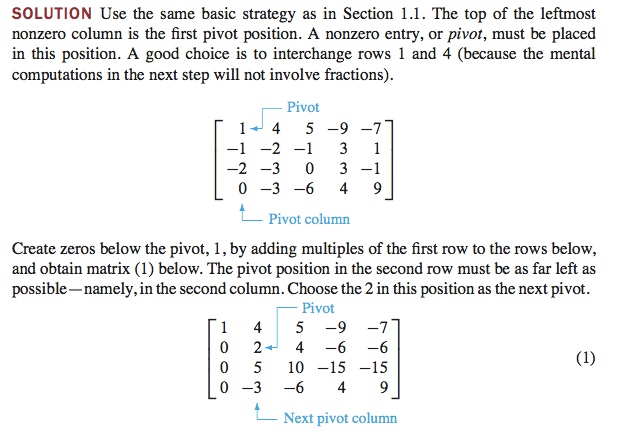
\includegraphics[scale=0.8]{figures_mvc/pivots_step_1}	
\end{center}

\begin{center}
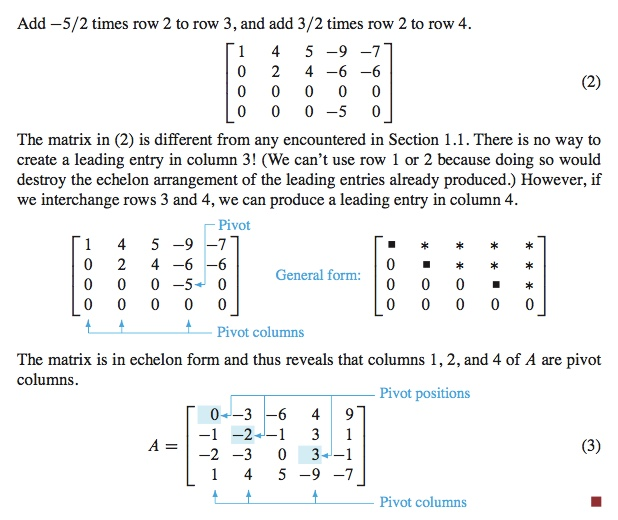
\includegraphics[scale=0.8]{figures_mvc/pivots_step_2}	
\end{center}
\end{example}

\subsection{Gauss-Jordan elimination}
In this section we introduce the \ti{Gauss-Jordan elimination} algorithm which will allow us to systematically reduce any matrix $A$ to its unique RREF, $U$. 

The algorithm consists of four steps, and it produces a matrix in REF. A fifth step produces a matrix in RREF. We illustrate the algorithm by an example.
 
\begin{align*}
	A=\begin{bmatrix}
		0 & 3 & -6 & 6 & 4 & -5 \\
		3 & -7 & 8 & -5 & 8 & 9 \\
		3 & -9 & 12 & -9 & 6 & 15
	\end{bmatrix}
\end{align*}

\begin{center}
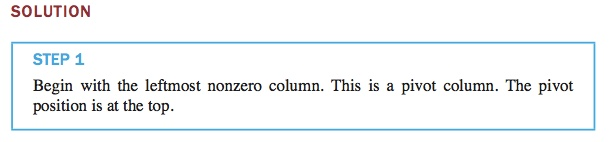
\includegraphics[scale=0.8]{figures_mvc/algo_step_1}	
\end{center}

\begin{center}
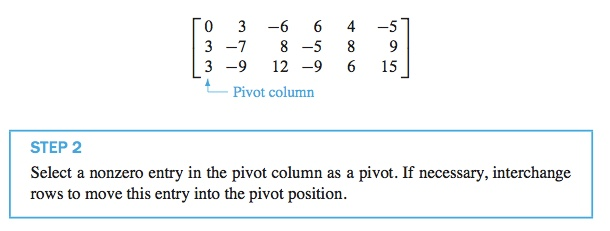
\includegraphics[scale=0.8]{figures_mvc/algo_step_2}	
\end{center}

\begin{center}
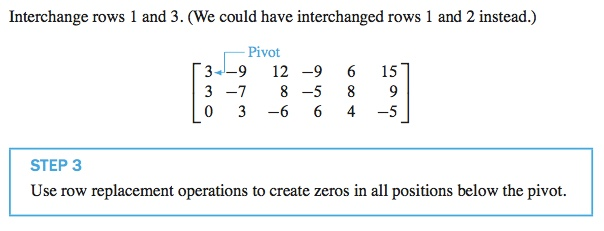
\includegraphics[scale=0.8]{figures_mvc/algo_step_3}	
\end{center}

\begin{center}
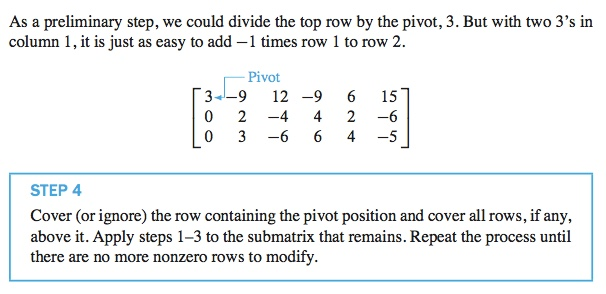
\includegraphics[scale=0.8]{figures_mvc/algo_step_4}	
\end{center}

\begin{center}
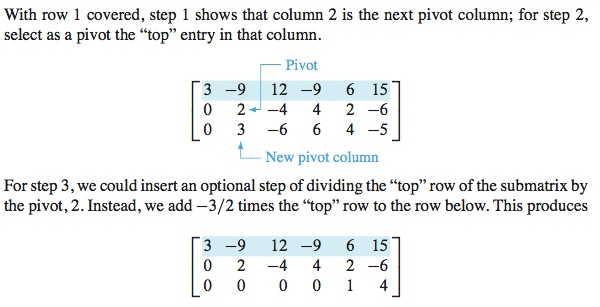
\includegraphics[scale=0.8]{figures_mvc/algo_step_5}	
\end{center}

\begin{center}
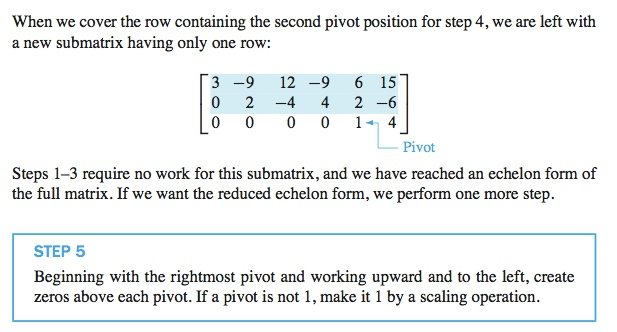
\includegraphics[scale=0.8]{figures_mvc/algo_step_6}	
\end{center}

\begin{center}
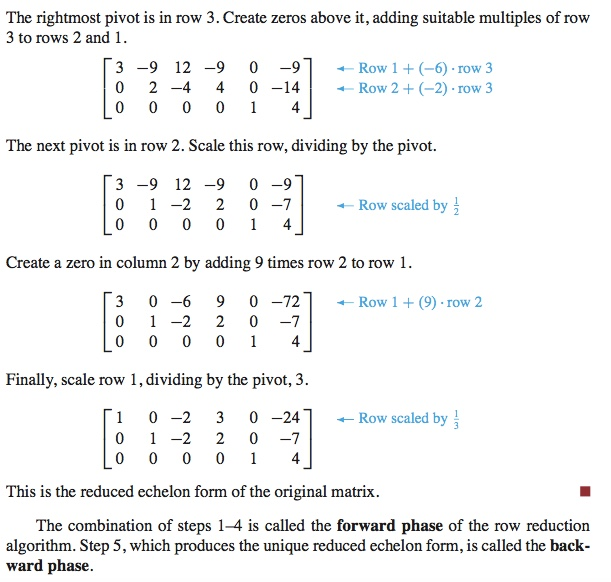
\includegraphics[scale=0.8]{figures_mvc/algo_step_7}	
\end{center}

\begin{exercise}
Row reduce the following matrices to RREF. Circle the pivot positions and pivot columns in the final matrix. \\
\vspace{0.25cm}
(a) $\begin{bmatrix}
	1 & 2 & 3 & 4 \\ 4 & 5 & 6 & 7 \\ 6 & 7 & 8 & 9
\end{bmatrix}$ \hspace{1.5cm} (b) $\begin{bmatrix}
	1 & 3 & 5 & 7 \\ 3 & 5 & 7 & 9 \\ 5 & 7 & 9 & 1
\end{bmatrix}$ \\
\vspace{0.25cm}
(c) $\begin{bmatrix}
	3 & -4 & 2 & 0 \\ -9 & 12 & -6 & 0 \\ -6 & 8 & -4 & 0
\end{bmatrix}$ \hspace{1.5cm} (d) $\begin{bmatrix}
	1 & -7 & 0 & 6 & 5 \\0 & 0 & 1 & -2 & -3 \\ -1 & 7 & -4 & 2 & 7
\end{bmatrix}$ 	
\end{exercise}

\subsection{Existence and uniqueness of solutions}
In this section we will answer the following two fundamental questions for any given linear system:
\begin{enumerate}
	\item Is the system consistent; that is, does at least one solution \ti{exist}.
	\item If a solution exists, is it the \ti{only} one; that is, is the solution \ti{unique}.
\end{enumerate}
\subsubsection{Homogeneous systems of linear equations}
A homogeneous system of linear equations $AX=0$ always has at least one solution, the \ti{trivial} solution, given by $x_1=x_2=\cdots=x_n=0$. Thus, \ti{a homogeneous system of linear equations is always consistent}. The fundamental question for a homogeneous system of linear equations is whether there exists a non-trivial solution.

Consider the system $RX=0$, where $R$ is an $m \times n$ matrix in reduced row echelon form. Let $1 \leq r \leq m$ and let $1,\cdots,r$ be the nonzero rows of $R$. The system $RX=0$ therefore consists of $r$ non-trivial equations. Letting $x_1,\cdots,x_r$ denote the first $r$ variables, and $u_i=x_{r+i}$, $i=1,\cdots,n-r$ denote the remaining $n-r$ free variables, the non-trivial equations take the form
\begin{align}
		x_1+\sum_{j=1}^{n-r}C_{1j}u_j&=0 \label{eq:non-triv_first} \\
		\vdots \hspace{1.8cm}& \hspace{0.5cm}\vdots \\
		x_r+\sum_{j=1}^{n-r}C_{rj}u_j&=0 \label{eq:non-triv_last}
	\end{align}
where each $x_i, i=1,\cdots,r$ occurs (with non-zero coefficient) only in the $i$th equation. All solutions to the system $RX=0$ are obtained by assigning any real numbers to $u_1,\cdots, u_{n-r}$ and then computing the values of $x_1,\cdots, x_r$ using \eqref{eq:non-triv_first} - \eqref{eq:non-triv_last}. This shows that \ti{if $r<n$, the system $RX=0$ has an infinite number of solutions}. \footnote{The $n \times n$ identity matrix is the $n \times n$ matrix for which each diagonal entry is 1, and each off-diagonal entry is 0. See Exercise \ref{ex:hom_system_examp} below for an example of this case.} If $r=n$, then $R$ is the $n \times n$ identity matrix and the system $RX=0$ has only the trivial solution. 

 We thus have the following theorem:

\begin{thm}[Solution sets of homogeneous linear systems]\label{thm:solution_sets_of_homogeneous_linear_systems} \hspace{10cm}
	\begin{enumerate}[(a)]
		\item If $A$ is an $m \times n$ matrix and $m<n$, then the homogeneous system of linear equations $AX=0$ has a non-trivial solution (in fact, an infinite number of them). 
		\item If $A$ is an $n \times n$ (square) matrix, then $A$ is row-equivalent to the $n \times n$ identity matrix if and only if the system of equations $AX=0$ has only the trivial solution. \footnote{If $m>n$, the system has a unique solution if and only if the reduced row echelon form the coefficient matrix is of the form
$
	\begin{bmatrix}
		1&0 \\ 0 & 1 \\ 0 & 0
	\end{bmatrix}.
$
}
	\end{enumerate}
\end{thm}

\begin{pf}
	\begin{enumerate}[(a)]
		\item Let $R$ be the unique RREF of the matrix $A$. Since $A$ and $R$ are row-equivalent, the systems $AX=0$ and $RX=0$ have exactly the same solutions. As before, let $r$ be the number of non-zero rows in $R$. Then $r \leq m$, and since $m < n$, we have $r<n$. We will therefore have $n-r>0$ free variables, so $AX=0$ has a non-trivial solution. 
		\item $(\implies)$ If $A$ is row-equivalent to $I$, then $AX=0$ and $IX=0$ have the same solutions, hence $AX=0$ has only the trivial solution $X=0$. \\
		$(\impliedby)$ Suppose $AX=0$ has only the trivial solution. Let $R$ be the unique RREF of $R$, and let $r$ be the number of non-zero rows of $R$. Since $R$ is row-equivalent to $A$, $RX=0$ has only the trivial solution. Thus $r \geq n$. But since $R$ has $n$ rows, $r \leq n$, and therefore $r=n$. Since $R$ is in RREF, it is the $n \times n$ identity matrix.
	\end{enumerate}
\end{pf}



\begin{exercise}\label{ex:hom_system_examp}
Consider the system $RX=0$ with coefficient matrix
\begin{align*}
	R=\begin{bmatrix}
		1&0&0&2&7 \\
		0&1&0&-1&3 \\
		0&0&1&-4&5 \\
		0&0&0&0&0 
	\end{bmatrix}
\end{align*}
Verify the following:
\begin{enumerate}[(a)]
	\item The system $RX=0$ consists of $r$ non-trivial equations and $m-r$ trivial equations. Write out these equations.
	\item Show that the non-trivial equations take the form \eqref{eq:non-triv_first} - \eqref{eq:non-triv_last}. Indentify the basic variables $x_1,\cdots,x_r$, the free variables $u_1,\cdots,u_{n-r}$, and the coefficients $C_{ij}$ in these equations.
	\item Find the solution set and express it in parametric form.
\end{enumerate}	
\end{exercise}

\subsubsection{Inhomogeneous systems of linear equations}
So far we have used elementary row operations to solve homogeneous systems of linear equations. What, then, do elementary row operations do toward solving an \emph{inhomogeneous} system of linear equations? Happily, it turns out that we solve an inhomogeneous system of linear equations in exactly the same way as a homogeneous one, with one minor modification.

\begin{defn}[Augmented matrix of an inhomogeneous linear system]\label{def:augmented_matrix}
The \ti{augmented matrix} of an inhomogeneous system of linear equations $AX=Y$ is the $m \times (n+1)$ matrix whose first $n$ columns are the columns of the coefficient matrix $A$ and whose last column is $Y$. We denote this matrix as $A'=[A|Y]$.
\end{defn}

\begin{example}\label{ex:augmented}
The augmented matrix of the inhomogeneous linear system
\begin{equation}\label{eq:inhom_system_example}
\begin{split}
	x_1-2x_2+x_3&=0 \\
	2x_2-8x_3&=8 \\
	5x_1-5x_3&=10 \\
\end{split}
\end{equation}
is given by \footnote{The vertical bar offsetting the final column in $A'$ has no meaning and is only there as a visual device to remind us that the matrix is an augmented matrix. Many authors do not typeset this vertical bar, and instead simply denote an augmented matrix exactly in the same way as a coefficient matrix. In this case, one determines whether the matrix is a coefficient matrix or augmented matrix from context.}
\begin{align*}
	A'=\left[\begin{array}{c c c | c}
		1&-2&1&0 \\
		0&2&-8&8 \\
		5&0&-5&10
	\end{array}\right]
\end{align*}	
\end{example}


Suppose we perform a sequence of elementary row operations on the coefficient matrix $A$ of an inhomogeneous linear system $AX=Y$, arriving at it's unique reduced row echelon form, $R$. If we perform the same operations on $A'$, we will arrive at a matrix $R'$ in reduced row echelon form, whose first $n$ columns are those of $R$ and whose last column is the $m \times 1$ matrix $Z$ which results from applying the same sequence of elementary row operations to the matrix $Y$. By the same arguments as before, the system $RX=Z$ is equivalent to the original system $AX=Y$, and therefore we can read off the solution set from $RX=Z$.

\begin{exercise}
Verify that performing Gauss-Jordan elimination on the augmented matrix $A'$ of Example \ref{ex:augmented} gives
\begin{align*}
	\left[\begin{array}{c c c | c}
		1&-2&1&0 \\
		0&2&-8&8 \\
		5&0&-5&10
	\end{array}\right] \to \left[\begin{array}{c c c | c}
		1&0&0&1 \\
		0&1&0&0 \\
		0&0&1&-1
	\end{array}\right]
\end{align*}
	
This shows that the inhomogeneous system \eqref{eq:inhom_system_example} has the unique solution $(x_1,x_2,x_3)=(1,0,-1)$.
\end{exercise}


Therefore, \ti{to solve an inhomogeneous linear system $AX=Y$, we simply reduce the augmented matrix $A'=[A|Y]$ to its unique reduced row-echelon form, $R'=[R|Z]$, using Gauss-Jordan elimination (exactly as we do for the coefficient matrix $A$ for a homogeneous system). We then read off the solution set from the equivalent system $RX=Z$.}

While a homogeneous system of linear equations is always consistent, this need not be the case for an inhomogeneous system, even if the number of equations is fewer than the number of unknowns.

\begin{example}
Consider the inhomogeneous linear system
	\begin{align}
		x_1+3x_2+7x_3&=2 \label{eq:inhom_inconsistent_1} \\
		-2x_1-6x_2-14x_3&=-3 \label{eq:inhom_inconsistent_2}
	\end{align}
Replacing \eqref{eq:inhom_inconsistent_2} by $2\eqref{eq:inhom_inconsistent_1}+\eqref{eq:inhom_inconsistent_2}$ gives $0=1$, which is false for any $(x_1,x_2,x_3)$, so the system is inconsistent.
\end{example}

\begin{example}
Consider now the inhomogeneous linear system $AX=Y$ with augmented matrix
\begin{equation}\label{eq:inhom_general_example}
A'=\left[\begin{array}{c c c | c}
		1&-2&1&y_1 \\
			2&1&1&y_2 \\
			0&5&-1&y_3
	\end{array}\right]
\end{equation}
We would like to know:
\begin{enumerate}
	\item Under what condition does the solution exist?
	\item If a solution exists, is it unique?
\end{enumerate}
Performing elementary row operations on $A'$, we arrive at the row echelon matrix
\begin{equation}
	\left[\begin{array}{c c c | c}
		1&-2&1&y_1 \\
			0&5&-1&-2y_1+y_2 \\
			0&0&0&2y_1-y_2+y_3
	\end{array}\right].
\end{equation}
We see that the system is consistent only if $2y_1-y_2+y_3=0$. In this case, $x_3$ is a free variable, so the system has an infinite number of solutions.
\end{example}

This example is illustrative of the general case.

\begin{thm}[Existence and uniqueness for inhomogeneous systems]\label{thm:existence_and_uniqueness_for_inhomogeneous_systems} \hspace{10cm}
\begin{enumerate}[(a)]
	\item An inhomogeneous linear system is consistent if and only if the rightmost column of its augmented matrix is \ti{not} a pivot column - that is, if and only if any echelon form of the matrix has \ti{no} row of the form
	$$[0 \ \cdots \ 0\  b] \ \text{ with $b$ nonzero.}$$
	\item If an inhomogeneous linear system is consistent, then the solution set contains either $(i)$ a unique solution, when there are no free variables, or $(ii)$ infinitely many solutions, when there is at least one free variable.
\end{enumerate}
\end{thm}

\begin{proof}
	Left to the reader. The details are very similar to the homogeneous case, with the obvious modifications.
\end{proof}

Before we close this section, let us take care of a piece of unfinished business and prove that every matrix $A$ has a unique RREF.

\begin{thm}[Uniqueness of reduced row echelon form]\label{thm:uniqueness_of_reduced_row_echelon_form}
	Every $m \times n$ matrix $A$ is row-equivalent to a \emph{unique} row-reduced echelon matrix $U$, called the \emph{reduced row echelon form of $A$}
\end{thm}

\begin{proof} \footnote{The following proof is due to W.H. Holzmann.}
	(By contradiction.) Suppose $A$ can be reduced by finite sequences of elementary row operations to two distinct $R$ and $S$, both in RREF. Since $R \neq S$, there must be a pair of indices $(i,j)$ such that $R_{ij} \neq S_{ij}$. Corresponding to $R$ and $S$, respectively, form new $m \times k$ matrices ($k \leq n$) $R'$ and $S'$ by selecting the first (leftmost) column for which $R$ and $S$ differ along with all pivot columns to the left of this column. \footnote{For instance, if $R=\begin{pmatrix}
		1 & 2 & 0 & 3 & 5 \\
		0 & 0 & 1 & 4 & 6 \\
		0 & 0 & 0 & 0 & 0
	\end{pmatrix}$ and $S=\begin{pmatrix}
		1 & 2 & 0 & 7 & 9 \\
		0 & 0 & 1 & 8 & 9 \\
		0 & 0 & 0 & 0 & 0
	\end{pmatrix}$, then $R'=\begin{pmatrix}
		1&0&3 \\ 0 & 1 & 4 \\ 0 & 0 & 0
	\end{pmatrix}$ and $S'=\begin{pmatrix}
		1&0&7 \\ 0 & 1 & 8 \\ 0 & 0 & 0
	\end{pmatrix}$.} Noting that the leftmost column in which $R$ and $S$ differ must be a non-pivot column, the matrices $R'$ and $S'$ must therefore take the form
	\begin{equation}\label{eq:uniqueness_of_rref}
		R'=
  \left(\begin{array}{c|c}
    I_n & \mathbf{r'} \\ \hline
    O & \mathbf{0} 
  \end{array}\right) \hspace{0.5cm} \text{ and } \hspace{0.5cm} S'=
  \left(\begin{array}{c|c}
    I_n & \mathbf{s'} \\ \hline
    O & \mathbf{0} 
  \end{array}\right).
\end{equation}
Note that $R'$ and $S'$ are both row-equivalent to $A$ (since $R$ and $S$ are row-equivalent to $A$ and deleting columns does not affect row-equivalence) and therefore to each other. 

Now interpret the matrices in \eqref{eq:uniqueness_of_rref} as augmented matrices. The system for $R'$ has a unique solution $\mathbf{r'}$, while the system for $S'$ has a unique solution $\mathbf{s'}$. Since the linear systems corresponding to row-equivalent matrices are equivalent, we must have $\mathbf{r'}=\mathbf{s'}$, which means $R'=S'$, and therefore $R=S$, which contradicts our assumption that these matrices are distinct. Hence, the RREF of $A$ must be unique.
\end{proof}


\subsection{Matrix operations}
In the preceding section, we viewed each elementary row operation as a function which takes as input a matrix and produces a new matrix. In the following sections, we will see that elementary row operations can equivalently be viewed as a function which takes as input \emph{two} matrices and returns a third matrix. This will lead us to define operations of addition and multiplication on \emph{entire matrices}, rather than on the just the rows of a matrix. We will also find it useful to define other operations on the set of matrices, which are not analogous to any familiar operations on the set of real numbers.
\subsubsection{Formal definition of a matrix}
In order to define operations on the set of matrices, it will help to take a slightly more formal view of a matrix. First, recall that a \emph{sequence} is just a function $f:\mathbb{N} \to \mathbb{R}$. \footnote{The notation $f:A \to B$ denotes a function $f$ from domain $A$ (the set of "inputs") to codomain $B$ (the set of "outputs") defined by $b=f(a)$ for all $a \in A$.} Denoting $f(n)$ by $f_n$, we visualize a sequence as a list of real numbers $(f_1,f_2,f_3,\cdots)$, indexed by $n \in \mathbb{N}$.

\begin{example}
Let $f:\mathbb{N} \to \mathbb{R}$ be defined by $f(n)=\frac{1}{n}$. Then we write the sequence $(f_1,f_2,f_3,\dots)=(1,\frac{1}{2},\frac{1}{3},\cdots)$.	
\end{example}

\begin{defn}[Matrix]\label{def:matrix}
Let $\overline{n}=\{1,2,\cdots,n\}$. A \emph{matrix} is a function $A:\overline{m} \times \overline{n} \to \mathbb{R}$.	
\end{defn}

As we did with sequences, we denote $A(i,j)$ by $A_{ij}$. We then visualize the matrix $A$ as the rectangular array of the numbers $A_{ij}$ with $m$ rows and $n$ columns. Two matrices are \emph{equal} if they have the same size and if each of the corresponding entries are equal.


\subsubsection{Matrix addition and scalar multiplication}
The definition of a matrix in \ref{def:matrix} makes it clear how to define addition and scalar multiplication of matrices; namely, we define these operations pointwise, the same way we always do for any function: 
\begin{align*}
	(f+g)(a) &=f(a)+g(a) \\
	(cf)(a) &=cf(a) 
\end{align*}

\begin{defn}[Matrix addition]
	If $A$ and $B$ are two $m \times n$ matrices, then the matrix $A+B$ has elements $(A+B)_{ij}=A_{ij}+B_{ij}$.
\end{defn}
Note that matrix addition is only defined if $A$ and $B$ are two matrices of the same size.
\begin{exercise}
	Let $A=\begin{bmatrix}
	4&0&5 \\ -1&3&2
\end{bmatrix}, B=\begin{bmatrix}
	1&1&1\\3&5&7
\end{bmatrix}$, and $C=\begin{bmatrix}
	2&-3 \\ 0&1
\end{bmatrix}$. Determine whether $A+B$ and $A+C$ are defined. If so, compute them.
\end{exercise}


\begin{defn}[Scalar multiplication of a matrix]
	If $A$ is an $m \times n$ matrix and $c$ is any scalar, then the matrix $cA$ has elements $(cA)_{ij}=cA_{ij}$.
\end{defn}

\begin{exercise}
Let $A$ and $B$ be the same as in the previous exercise. Compute $2B$ and $A-2B$.	
\end{exercise}

The usual rules of algebra apply to sums and scalar multiples of matrices, as the next theorem shows.

\begin{thm}[Properties of matrix addition and scalar multiplication]\label{thm:matrix_add_scalar_multiply_properties}
Let $A,B,$ and $C$ be matrices of the same size, and let $r$ and $s$ be scalars.
	\begin{enumerate}[(i)]
		\item $(A+B)+C=A+(B+C)$ (matrix addition is associative)
		\item $A+0=A$ (the zero matrix is an additive identity)
		\item Each matrix $A$ has an additive inverse $-A$ such that $A-A=0$.
		\item $A+B=B+A$ (matrix addition is commutative) 
		\item $r(A+B)=rA+rB$ (scalar multiplication distributes over matrix addition)
		\item $(r+s)A=rA+sA$ (scalar multiplication distributes over scalar addition)
		\item $r(sA)=(rs)A$ (associativity of scalar multiplication)
	\end{enumerate}
	These properties are exactly the same properties of addition and scalar multiplication of vectors. Indeed, we can view a vector in $\R^n$ as an $n \times 1$ (or $1 \times n$) matrix. \footnote{In Section \ref{sec:vector_spaces}, we will see other sets which admit operations of addition and scalar multiplication which behave exactly like those of vectors. This will lead to the notion of an abstract \emph{vector space}.}
\end{thm}


\begin{pf}
For each of these we need to show that $(1)$ the matrix on the left and right hand side of each equation has the same size, and $(2)$ each of the corresponding entries are equal. Condition $(1)$ holds for each since $A,B,$ and $C$ are all the same size. Condition $(2)$ holds in each case because of the corresponding properties of real numbers. For example, property $(iv)$ holds for matrices $A$ and $B$ since $A_{ij}+B_{ij}=B_{ij}+A_{ij}$ holds for real numbers $A_{ij}$ and $B_{ij}$. The remaining properties are checked similarly and are left as an exercise.
\end{pf}

\begin{exercise}
Prove properties (ii)-(vii) in Theorem \ref{thm:matrix_add_scalar_multiply_properties}.	
\end{exercise}

\subsubsection{Matrix multiplication}\label{sec:matrix_multiplication}
We have seen in the previous sections that the process of forming linear combinations of the rows of a matrix is a fundamental one. We now introduce a systematic way of doing this. 

Let $B$ be an $m \times n$ matrix with rows $\beta_1,\beta_2,\cdots, \beta_m$. Denote the $j$th entry of the $i$th row by $B_{ij}$. For example, if
\begin{align*}
	B=\begin{bmatrix}
		1&2&3 \\ 4&5&6
	\end{bmatrix}
\end{align*}
then $m=2, n=3, \beta_1=(1,2,3), B_{12}=2$, etc. 
Suppose we form a new $m \times n$ matrix $C$ whose rows $\gamma_1,\gamma_2, \cdots, \gamma_m$ are linear combinations of the rows of $B$. For example, if we take $B$ as above and let \footnote{These are not elementary row operations. We are just taking arbitrary linear combinations here.}
\begin{align*}
	\gamma_1&=2\beta_1-\beta_2, \\
	\gamma_2&=\beta_1+2\beta_2,
\end{align*}

then 

\begin{align*}
	C=\begin{bmatrix}
		2(1,2,3)-1(4,5,6) \\
		(1,2,3)+2(4,5,6)
	\end{bmatrix}=\begin{bmatrix}
		-2&-1&0 \\ 9 & 12 & 15
	\end{bmatrix}.
\end{align*}

Denoting the $i$th multiple of $j$th row of $B$ by $A_{ij}$, from the matrix above on the left we see that the rows of $C$ take the form
\begin{align*}
	\gamma_1&=A_{11}\beta_1+A_{12}\beta_2=\sum_{j=1}^2A_{1j}\beta_j, \\
	\gamma_2&=A_{21}\beta_1+A_{22}\beta_2=\sum_{j=1}^2A_{2j}\beta_j.
\end{align*}

Thus, the rows of $C$ are determined by 4 scalars which are themselves entries in a $2 \times 2$ matrix
\begin{align*}
	A=\begin{bmatrix}
		A_{11} & A_{12} \\
		A_{21} & A_{22}
	\end{bmatrix}=\begin{bmatrix}
		2 & -1 \\
		1 & 2
	\end{bmatrix}.
\end{align*}

Letting $C_{ik}$ denote the $k$th entry of the $i$th row of $C$, we see that $C_{ik}=\sum_{j=1}^2A_{ij}B_{jk}$. This is precisely the formula for the dot product of the $i$th row of $A$ with the $j$th column of $B$, viewing each as a vector in $\R^2$. For example, $C_{11}=A_{11}B_{11}+A_{12}B_{21}=2(1)+(-1)(4)=-2$.

Generalizing this example, we wish to define the \emph{product} of two matrices $A$ and $B$ to be the matrix $C$ whose $ij$-entry $C_{ij}$ is the dot product of the $i$th row of $A$ with the $j$th column of $B$. We note immediately that, for this to make sense, the matrices $A$ and $B$ must be compatible sizes, in the sense that the set of rows of $A$ and the set of columns of $B$ must each consist of vectors of the same length, otherwise the dot products will not be defined. This leads us to the following definition.

\begin{defn}[Matrix multiplication]\label{def:matrix_multiplication}
	Let $A$ be an $m \times n$ matrix and $B$ be an $n \times p$ matrix. The \ti{product} of $A$ and $B$ is the $m \times p$ matrix $C$ whose $(i,j)$-entry is $C_{ij}=\sum_{k=1}^n A_{ik}B_{kj}$, which is the dot product of the $i$th row of $A$ with the $j$th column of $B$.
\end{defn}

\begin{example}[Row-column rule for matrix multiplication]
	One can remember this definition by the following ``row-column" rule for computing $AB$: the entry in row $i$ and column $j$ of $AB$ is the sum of the products of corresponding entries from row $i$ of $A$ and column $j$ of $B$. That is, the $(i,j)$-entry of $AB$ is given by
\begin{equation}
	(AB)_{ij}=A_{i1}B_{1j}+A_{i2}B_{2j}+\cdots+A_{in}B_{nj}	
\end{equation}

\end{example}



\begin{example}
Taking $A$ and $B$ to be the matrices
\begin{align*}
	A&=\begin{bmatrix}
			2&-1\\1&3\\-2&6
		\end{bmatrix}, \\
	B&=	\begin{bmatrix}
		5&-1&2 \\ 15&4&8
	\end{bmatrix},
\end{align*}
their product is  
\begin{align*}
	C&=AB \\
	&=\begin{bmatrix}
			2&-1\\1&3\\-2&6
		\end{bmatrix}\begin{bmatrix}
		5&-1&2 \\ 15&4&8
	\end{bmatrix} \\
	&=\begin{bmatrix}
		-5&-6&-4 \\
		50&11&26 \\
		80&22&44
	\end{bmatrix}
\end{align*}
\end{example}

As discussed above, the product of these matrices is defined since the length of the rows (or, equivalently, the number of \emph{columns}) in the first matrix coincides with the length of the columns (or, equivalently, the number of \emph{rows}) in the second matrix. In this case, multiplying an $3 \times 2$ matrix and a $2 \times 3$ matrix gave a $3 \times 3$ matrix.

\begin{exercise}
	If $A$ is a $3 \times 5$ matrix and $B$ is a $5 \times 2$ matrix, what are the sizes of $AB$ and $BA$, if they are defined?	
\end{exercise}

\begin{exercise}
Let $A=\begin{bmatrix}
	2&3\\1&-5
\end{bmatrix}$ and $B=\begin{bmatrix}
	4&3&6 \\1&-2&3
\end{bmatrix}$. Compute $AB$.	
\end{exercise}

Note that this definition of matrix multiplication agrees with our notation $AX=Y$ for a linear system of equations: $A$ is an $m \times n$ matrix, $X$ is an $ n \times 1$ matrix, and $Y$, which is the product of $A$ and $X$ is an $m \times 1$ matrix. 
	\begin{align*}
		\begin{bmatrix}
			A_{11} & A_{12} & \cdots & A_{1n} \\
			\vdots & &  & \vdots \\
			A_{m1} & A_{m2} & \cdots & A_{mn}
		\end{bmatrix}\begin{bmatrix}
			x_1 \\ x_2 \\ \vdots \\ x_n
		\end{bmatrix}=\begin{bmatrix}
			y_1 \\ y_2 \\ \vdots \\ y_m
		\end{bmatrix}
	\end{align*}

\begin{thm}[Properties of matrix multiplication]\label{thm:properties_of_matrix_multiplication}
	Let $A$ be an $m \times n$ matrix, and let $B$ and $C$ have sizes for which the indicated sums and products are defined. Then the following hold for all such matrices $A,B,$ and $C$.
\begin{enumerate}[(i)]
	\item $(AB)C=A(BC)$ (associative law of multiplication)
	\item $A(B+C)=AB+AC$ (left distributive law)
	\item $(B+C)A=BA+CA$ (right distributive law)
	\item $r(AB)=(rA)B=A(rB)$ for any scalar $r$
	\item $I_mA=A=AI_n$ (identity for matrix multiplication)
\end{enumerate}
\end{thm}

\begin{pf}
As before, for each of these we need to check that (1) both sides are matrices of the same size, and (2) the corresponding matrix elements on each side are all equal. 

(i) For $AB$ to be defined, $B$ must be an $n \times p$ matrix, for some $p$. Then, for $BC$ to be defined, $C$ must be $p \times q$ matrix. We therefore have 
\begin{align*}
	AB: (m \times n)(n \times p)&=m \times p \\
	BC: (n \times p)(p \times q)&=n \times q
\end{align*}
so
\begin{align*}
	(AB)C: (m \times p)(p \times q)&=m \times q \\
	A(BC): (m \times n)(n \times q)&=m \times q
\end{align*}
hence both sides have the same size. \\
\\

Applying the definition of matrix multiplication, we have
\begin{align*}
	[(AB)C]_{ij}&=\sum_{\ell=1}^p(AB)_{i\ell}C_{\ell j} \\
	&=\sum_{\ell=1}^p\sum_{k=1}^n (A_{ik}B_{k\ell})C_{\ell j} \\
	&=\sum_{\ell=1}^p\sum_{k=1}^n A_{ik}(B_{k\ell}C_{\ell j}) \text{ (by associativity in $\mathbb{R}$)}\\
	&=\sum_{k=1}^nA_{ik}(BC)_{kj} \\
	&=[A(BC)]_{ij},
\end{align*}
so the corresponding entries are equal, showing that (i) holds. Properties (ii) - (v) are checked similarly, and are left as exercises.	
\end{pf}

\begin{defn}[Power of a matrx]
	If $A$ is an $n\times n$ matrix and $k$ is a positive integer, then the \ti{$k$th power of $A$}, $A^k$, is the product of $k$ copies of $A$:
\begin{align*}
	A^k=\underbrace{A \cdots A}_{\text{$k$ times}}.
\end{align*}
Since matrix multiplication is associative, there is no need to insert parenthesis into the expression above.
\end{defn}

We have seen in theorem Theorem \ref{thm:properties_of_matrix_multiplication} that some of the properties of multiplication of real numbers also hold for matrices (e.g., associativity). However, it is not true that \emph{all} such properties hold for matrix multiplication, as the next three examples show.

\begin{example}[Matrix multiplication is not commutative] 
If $A$ is a $3 \times 2$ matrix and $B$ is a $2 \times 4$ matrix, then their product is a $3 \times 4$ matrix. However, the product $BA$ is not even defined, since the sizes are not compatible! This shows that matrix multiplication is not commutative. Even if we choose $A$ and $B$ such that both $AB$ and $BA$ are defined, these might not be equal. For instance, let $A=\begin{bmatrix}
		5&1\\3&-2
	\end{bmatrix}$ and $B=\begin{bmatrix}
		2&0 \\ 4&3
	\end{bmatrix}$. Then $AB=\begin{bmatrix}
	16 & 9 \\ -18 & -15
\end{bmatrix}$ and  $BA=\begin{bmatrix}
	4 & 6 \\ 11 & -3
\end{bmatrix}$. Hence $AB$ and $BA$ are both defined, but $AB \neq BA$.
\end{example}

\begin{example}[Matrix multiplication does not satisfy the cancellation laws]
For real numbers, the cancellation law says that if $AB=AC$, then $B=C$. This does not hold, in general, for matrices. As an example, let $A=\begin{bmatrix}
		2&-3\\-4&6
	\end{bmatrix},$ $B=\begin{bmatrix}
		8&4\\5&5
	\end{bmatrix},$ and $C=\begin{bmatrix}
		5&-2\\3&1
	\end{bmatrix}$.	We see that $AB=BC=\begin{bmatrix}
	1 & -7 \\ -2 & 14
\end{bmatrix}$, but $B \neq C$. One can show similarly that the other cancellation law ($BA=CA \implies B=C$) \footnote{Note that the two cancellation laws are not equivalent  here since matrix multiplication is not commutative.} also does not hold in general for matrices.
\end{example}

\begin{example}[Zero products do not imply one matrix is zero]
	For real numbers, if $AB=0$ then either $A=0$ or $B=0$. To see that this does not hold, in general, for matrices, let $A=\begin{bmatrix}
		3&-6 \\ -1&2
	\end{bmatrix}$ and $B=\begin{bmatrix}
	2 & 2 \\ 1 & 1
\end{bmatrix}$. Then $AB=0$, but neither $A$ nor $B$ is the zero matrix. 
\end{example}

We now define two operations which are not analogous to any familiar operations on the set of real numbers.

\subsubsection{Transpose of a matrix}
\begin{defn}[Transpose of a matrix]
	Given an $m \times n$ matrix $A$, the \ti{transpose} of $A$ is the $n \times m$ matrix, denoted $A^T$, whose columns are formed from the corresponding rows of $A$, that is, given $A$, $A^T$ is the matrix with elements $(A^T)_{ij}=A_{ji}$. 
\end{defn}

\begin{example}
	If $A=\begin{bmatrix}
	-5&2\\1&-3 \\ 0&4
\end{bmatrix}$, then $A^T=\begin{bmatrix}
	-5&1&0 \\ 2&-3&4
\end{bmatrix}$.
\end{example}

\begin{thm}[Properties of $A^T$]\label{thm:transpose_properties}
	Let $A$ and $B$ be matrices whose sizes are appropriate for the following sums and products to be defined. Then
\begin{enumerate}[(i)]
	\item $(A^T)^T=A$
	\item $(A+B)^T=A^T+B^T$
	\item For any scalar $r$, $(rA)^T=rA^T$
	\item $(AB)^T=B^TA^T$
\end{enumerate}
\end{thm}

\begin{pf}
Clearly the matrices on each side are the same size since $A$ and $B$ are the same size. All that is left is to check that the corresponding matrix elements are equal in each case. We will do this for (iv). The proofs for (i)-(iii) are checked similarly, and are left as exercises. 
\begin{align*}
	[(AB)^T]_{ij}&=(AB)_{ji} \\
	&=\sum_{k=1}^n A_{jk}B_{ki} \\
	&=\sum_{k=1}^n B_{ki}A_{jk} \ (\text{by commutativity in } \mathbb{R}) \\
	&=\sum_{k=1}^n B^T_{ik}A^T_{kj} \\
	&=[B^TA^T]_{ij}	
\end{align*}
This proves property (iv).
\end{pf}

\begin{exercise}
Prove properties (i)-(iii) of Theorem \ref{thm:transpose_properties}.	
\end{exercise}


\subsubsection{Trace of a matrix}
There is another useful property defined for \emph{square} ($n \times n$) matrices.

\begin{defn}[Trace of a matrix]
	The \emph{trace} of an $n \times n$ matrix $A$ is the sum of its diagonal entries:
	\begin{align*}
		\text{Tr }A=\sum_{i=1}^n A_{ii}.
	\end{align*}
\end{defn}

\begin{example}
Let $A=\begin{bmatrix}
	1&2&3 \\ 4 & 5 & 6 \\ 7 & 8 & 9
\end{bmatrix}$. Then
\begin{align*}
	\text{Tr }A=1+5+9=15.
\end{align*}	
\end{example}

\begin{thm}[Properties of the trace]\label{thm:trace_properties}
	Let $A,B$ be $n \times n$ matrices and $c$ a scalar. Then
	\begin{enumerate}[(i)]
		\item $\Tr (A+B)=\Tr A + \Tr B$,
		\item $\Tr(cA)=c\Tr A$, 
		\item $\Tr A^T=\Tr A$,
		\item $\Tr AB= \Tr BA$,
	\end{enumerate}
\end{thm}

\begin{exercise}
Prove Theorem \ref{thm:trace_properties}.	
\end{exercise}

\subsection{Invertible matrices}
\subsubsection{Elementary matrices}
We will now see that elementary row operations can be represented by multiplication by matrices. 

\begin{defn}[Elementary matrix]\label{def:elementary_matrix}
	An $n \times n$ (square) matrix is said to be an \emph{elementary matrix} if it can be obtained from the $n \times n$ identity matrix by means of a single elementary row operation.
\end{defn}

\begin{exercise}\label{ex:2_by_2_elementary_matrices}
Let $c$ be a constant. Verify that the complete list of $2 \times 2$ elementary matrices is 
	\begin{align*}
	\begin{bmatrix}
		0 & 1 \\ 1 & 0
	\end{bmatrix}, \begin{bmatrix}
		1 & c \\ 0 & 1
	\end{bmatrix}, \begin{bmatrix}
		1 & 0 \\ c & 1
	\end{bmatrix}, 
	 \begin{bmatrix}
		c & 0 \\ 0 & 1
	\end{bmatrix} (c \neq 0), \begin{bmatrix}
		1 & 0 \\ 0 & c
	\end{bmatrix} (c \neq 0).
\end{align*}
\end{exercise}

\begin{thm}[Elementary row operations are represented by elementary matrices]
If $e$ is an elementary row operation and $E$ the $n \times n$ elementary matrix $E=e(I)$, then for every $m \times n$ matrix $A$, $e(A)=EA$.	
\end{thm}

\begin{pf}
We consider each type of elementary row operation separately.

(i) Suppose $r \neq s$ and let $e$ be the elementary row operation which replaces row $r$ by row $r$ plus $c$ times row $s$. We need to show that $EA=e(A)$. We can write the elements of the corresponding elementary matrix $E$ as \footnote{In the following $\delta_{ij}$ denotes the $ij$-component of the identity matrix; that is, $\delta_{ij}=1$ if $i=j$ and $\delta_{ij}=0$ if $i \neq j$.}
	 \begin{align*}
	 	E_{ik}=\begin{cases}
	 		\delta_{ik}, &i \neq r \\
	 		\delta_{rk}+c\delta_{sk}, &i=r.
	 	\end{cases}
	 \end{align*}
Then, if $i \neq r$, 
\begin{align*}
	(EA)_{ij}=\sum_{k=1}^m E_{ik}A_{kj} = \sum_{k=1}^m\delta_{ik}A_{kj}=A_{ij}
\end{align*}
and for $i=r$,
\begin{align*}
	(EA)_{rj}=\sum_{k=1}^m E_{rk}A_{kj} =\sum_{k=1}^m(\delta_{rk}+c\delta_{sk})A_{kj} =A_{rj}+cA_{sj}
\end{align*}
which shows $EA=e(A)$, as desired.

(ii) Suppose $r \neq s$ and let $e$ be the elementary row operation which exchanges rows $r$ and $s$. The elements of the corresponding elementary matrix are given by
	 \begin{align*}
	 	E_{ik}=\begin{cases}
	 		\delta_{ik}, &i \neq r,s \\
	 		\delta_{rk}, &i=s \\
	 		\delta_{sk}, &i=r.
	 	\end{cases}
	 \end{align*}
Then, if $i \neq r,s$, 
\begin{align*}
	(EA)_{ij}=\sum_{k=1}^m E_{ik}A_{kj} = \sum_{k=1}^m\delta_{ik}A_{kj}=A_{ij}
\end{align*}
if $i=r$,
\begin{align*}
	(EA)_{rj}=\sum_{k=1}^m E_{rk}A_{kj} =\sum_{k=1}^m\delta_{sk}A_{kj} =A_{sj}
\end{align*}
and if $i=s$,
\begin{align*}
	(EA)_{sj}=\sum_{k=1}^m E_{sk}A_{kj} =\sum_{k=1}^m\delta_{rk}A_{kj} =A_{rj}
\end{align*}
which shows $EA=e(A)$.

(iii) Let $e$ be the elementary row operation which multiplies rows $r$ by $c$, $c\neq 0$. We need to show that $EA=e(A)$. The corresponding elementary matrix can be written as 
	 \begin{align*}
	 	E_{ik}=\begin{cases}
	 		\delta_{ik}, &i \neq r \\
	 		c\delta_{rk}, &i=r. 
	 	\end{cases}
	 \end{align*}
Then, if $i \neq r$, 
\begin{align*}
	(EA)_{ij}=\sum_{k=1}^m E_{ik}A_{kj} = \sum_{k=1}^m\delta_{ik}A_{kj}=A_{ij}
\end{align*}
if $i=r$,
\begin{align*}
	(EA)_{rj}=\sum_{k=1}^m E_{rk}A_{kj} =\sum_{k=1}^m(c\delta_{rk})A_{kj} =cA_{rj}
\end{align*}
which shows $EA=e(A)$.	
\end{pf}

\begin{exercise}
\begin{enumerate}[(a)]
    \item Let $E=\begin{bmatrix} 1 & 0 \\ -3 & 1 \end{bmatrix}$ be the elementary matrix obtained from the $2 \times 2$ identity matrix by replacing $R2 \mapsto R2-3R1$. Consider the matrix $A=\begin{bmatrix} 1& 2 \\ 3 & 4 \end{bmatrix}$. Show that the matrix product $EA$ is equal to the result of performing the row replacement $R2 \mapsto R2-3R1$ on $A$.
    \item Let $E=\begin{bmatrix} 0 & 1 \\ 1 & 0 \end{bmatrix}$ be the elementary matrix obtained from the $2 \times 2$ identity matrix by the interchange $R1 \leftrightarrow R2$. Consider the matrix $A=\begin{bmatrix} 1& 2 \\ 3 & 4 \end{bmatrix}$. Show that the matrix product $EA$ is equal to the result of interchanging the two rows of $A$.
\end{enumerate}
\end{exercise}


\begin{cor}
Let $A$ and $B$ be $m \times n$ matrices. Then $B$ is row-equivalent to $A$ if and only if $B=PA$, where $P$ is a product of $m \times m$ elementary matrices.	
\end{cor}

\begin{pf}
$(\implies)$ Suppose $B$ is row-equivalent to $A$. Let $E_1, E_2, \cdots, E_s$ be the elementary matrices corresponding to some sequence of elementary row operations which carries $A$ into $B$. Then $B=(E_s \cdots E_2 E_1)A$.

$(\impliedby)$ Suppose $B=PA$ where $P=E_s \cdots E_2E_1$ and the $E_i$ are $m \times m$ elementary matrices. Then $E_1 A$ is row-equivalent to $A$, and $E_2(E_1 A)$ is row-equivalent to $E_1 A$, so by transitivity $E_2E_1A$ is row-equivalent to $A$. It follows by induction that $(E_s \cdots E_1)A$ is row-equivalent to $A$.	
\end{pf}

\begin{exercise}
Let $E_1=\begin{bmatrix}
	1&0&0 \\ 0&1&0 \\ -4&0&1
\end{bmatrix}, E_2=\begin{bmatrix}
	0&1&0 \\ 1&0&0 \\ 0&0&1
\end{bmatrix}$, and $E_3=\begin{bmatrix}
	1&0&0 \\ 0&1&0 \\ 0&0&5
\end{bmatrix}$, and let $A$ be an arbitrary $3 \times 3$ matrix. Compute 
$E_1A, E_2A,$ and $E_3A$, and describe how these products can be obtained by elementary row operations on $A$.	
\end{exercise}

\subsubsection{Invertible matrices}
Suppose $P$ is an $m \times m$ matrix which is a product of elementary matrices. Then, for each $m \times n$ matrix $A$, the matrix $B=PA$ is row-equivalent to $A$. By symmetry (see Lemma \ref{lem:row_equivalence_is_an_equivalence_relation}), $A$ is therefore row-equivalent to $B$ and there is a product $Q$ of elementary matrices such that $A=QB$. In particular, this is true when $A$ is the $m \times m$ identity matrix. 

In other words, there is an $m \times m$ matrix $Q$, which is itself a product of elementary matrices, such that $QP=I$. As we shall soon see, the existence of a $Q$ with $QP=I$ is equivalent to the fact that $P$ is a product of elementary matrices.

\begin{defn}[Invertible matrix]
	Let $A$ be an $n \times n$ matrix. An $n \times n$ matrix $B$ such that $BA=I$ is called a \emph{left inverse} of $A$; an $n \times n$ matrix $B$ such that $AB=I$ is called a \emph{right inverse} of $A$. If $AB=BA=I$, then $B$ is called a \emph{two-sided inverse} (or just \emph{inverse}) of $A$ and $A$ is said to be \emph{invertible} or \emph{non-singular}. A matrix which is not invertible is called a \emph{singular} matrix.
\end{defn}

\begin{exercise}
Let $A=\begin{bmatrix}
	2&5 \\ 3&8
\end{bmatrix}$ and $B=\begin{bmatrix}
	8&-5 \\ -3&2
\end{bmatrix}$. Show that $B$ is a two-sided inverse for $A$.	
\end{exercise}

\begin{thm}[Uniqueness of inverses]\label{thm:uniqueness_of_inverses}
	If $A$ has a left inverse $B$ and a right inverse $C$, then $B=C$. 
\end{thm}

\begin{pf}
Suppose $BA=I$ and $AC=I$. Then
\begin{align*}
	B=BI=B(AC)=(BA)C=IC=C. 
\end{align*}	
\end{pf}

Theorem \ref{thm:uniqueness_of_inverses} says that if a matrix $A$ has a left inverse and a right inverse, then these must be equal. In particular, if $A$ has a two-sided inverse, this theorem shows that it is unique. We denote the unique two-sided inverse by $A^{-1}$ and call it \emph{the} inverse of $A$.

\begin{thm}[Properties of $A^{-1}$]\label{thm:properties_of_A_inverse} \hspace{10cm}
		\begin{enumerate}[(i)]
		\item If $A$ is invertible, so is $A^{-1}$ and $(A^{-1})^{-1}=A$.
		\item If both $A$ and $B$ are invertible, so is $AB$, and $(AB)^{-1}=B^{-1}A^{-1}$.
		\item If $A$ is invertible, so is $A^T$ and $(A^T)^{-1}=(A^{-1})^T$.
	\end{enumerate}
\end{thm}

\begin{pf} 
(i) Follows immediately from the symmetry of the definition. 

(ii) $(B^{-1}A^{-1})(AB)=B^{-1}(A^{-1}A)B=B^{-1}B=I$. By uniqueness of inverses, $(AB)^{-1}=B^{-1}A^{-1}$.

(iii) $(A^{-1})^TA^T=(AA^{-1})^T=I^T=I$. By uniqueness of inverses, $(A^{-1})^T=(A^T)^{-1}$. 

Generalizing (ii), any finite product of invertible matrices is invertible, with inverse
\begin{align*}
	(A_1A_2\cdots A_s)=A_s^{-1} \cdots A_2^{-1}A_1^{-1}
\end{align*}	
\end{pf}

\begin{thm}[Elementary matrices are invertible]\label{thm:elementary_matrices_are_invertible}
An elementary matrix $E$ is invertible. The inverse of $E$ is the elementary matrix of the same type that transforms $E$ back into $I$.
\end{thm}

\begin{pf}
Let $E$ be the elementary matrix corresponding to the elementary row operation $e$. If $e'$ is the inverse operation of $e$ and $E'=e'(I)$, then $EE'=e(E')=e(e'(I))=I$, so $E$ is invertible and $E'=E^{-1}$.	
\end{pf}

\begin{example}
\begin{enumerate}[(a)]
	\item $\begin{bmatrix}
		0&1 \\ 1&0
	\end{bmatrix}^{-1}=  \begin{bmatrix}
		0 & 1 \\ 1 & 0
	\end{bmatrix}$
	\item $\begin{bmatrix}
		1&c \\ 0&1
	\end{bmatrix}^{-1}= \begin{bmatrix}1 & -c \\ 0 & 1 \end{bmatrix}$
	\item $\begin{bmatrix}
		1&0 \\ c&1
	\end{bmatrix}^{-1}=\begin{bmatrix}
		1 & 0 \\ -c & 1
	\end{bmatrix}$
	\item When $c \neq 0$,
	$\begin{bmatrix}
		c&0 \\ 0&1
	\end{bmatrix}^{-1}=\begin{bmatrix}
		c^{-1} & 0 \\ 0 & 1
	\end{bmatrix},$ \hspace{0.5cm} $\begin{bmatrix}
		1&0 \\ 0 &c
	\end{bmatrix}^{-1}= \begin{bmatrix}
		1 & 0 \\ 0 & c^{-1}
	\end{bmatrix}.$
\end{enumerate}
\end{example}

\begin{thm}[Invertible matrix theorem]\label{thm:invertible_matrix_theorem}
	If $A$ is an $n \times n$ matrix, the following are equivalent.
	\begin{enumerate}[(i)]
		\item $A$ is invertible.
		\item $A$ is row-equivalent to the $n \times n$ identity matrix.
		\item $A$ is a product of elementary matrices.
	\end{enumerate} 	
\end{thm}

\begin{pf}
We will show that $(i) \implies (ii) \implies (iii) \implies (i)$. Assume $(i)$ is true. Let $R$ be the RREF of $A$. Then $R=E_k\cdots E_2 E_1 A$, where $E_1,\cdots,E_k$ are elementary matrices. Since each $E_j$ is invertible, we have $A=E_1^{-1} \cdots E_k^{-1}R$. Since products of invertible matrices are invertible, we see that $A$ is invertible if and only if $R$ is invertible. Since $R$ is a square matrix in RREF, $R$ is invertible iff it is the $n \times n$ identity matrix (otherwise, it would have a row of zeros; we will prove in section \ref{sec:determinants} that any such matrix is singular). Hence, $(i) \implies (ii)$. $(iii)$ follows immediately from $(ii)$. $(i)$ follows immediately from $(iii)$ by Theorem \ref{thm:properties_of_A_inverse}.	
\end{pf}

\begin{cor}[How to compute $A^{-1}$]\label{cor:how_to_compute_a_inverse}
If $A$ is an invertible $n \times n$ matrix and if a sequence of elementary row operations reduces $A$ to the identity, then that same sequence of operations when applied to $I$ yields $A^{-1}$.	
\end{cor}

\begin{pf}
If $E_k \cdots E_1 A=I$, where each $E_j$ is an elementary matrix, then multiplying both sides on the right by $A^{-1}$ gives $E_k \cdots E_1 I=A^{-1}$.	
\end{pf}

Corollary \ref{cor:how_to_compute_a_inverse} gives an algorithm to compute $A^{-1}$: we simply row reduce the augmented matrix $[A|I]$. If $A$ is row-equivalent to $I$, then $[A|I]$ is row-equivalent tp $[I|A^{-1}]$. Otherwise, $A$ does not have an inverse.

\begin{example}
We find the inverse of the matrix $A=\begin{bmatrix}
	0&1&2 \\ 1&0&3 \\ 4&-3&8
\end{bmatrix}$ by performing Gauss-Jordan elimination on the augmented matrix
\begin{align*}
\left[	\begin{array}{c c c | c c c}
		0 & 1 & 2 & 1 & 0 & 0 \\
		1 & 0 &3 & 0 & 1 & 0 \\
		4 & -3 & 8 & 0 & 0 & 1
	\end{array}\right],
\end{align*} which gives \begin{align*}
\left[	\begin{array}{c c c | c c c}
		1 & 0 & 0 & -\frac{9}{2} & 7 & -\frac{3}{2} \\
		0 & 1 & 0 & -2 & 4 & -1 \\
		0 & 0 & 1 & \frac{3}{2} & -2 & \frac{1}{2} 
	\end{array}\right]
\end{align*}
so $A^{-1}=\begin{bmatrix}
	-\frac{9}{2} & 7 & -\frac{3}{2} \\
	-2 & 4 & -1 \\
	\frac{3}{2} & -2 & \frac{1}{2}
\end{bmatrix}$.	
\end{example}

\begin{exercise}
Find the inverse of the matrix $A=\begin{bmatrix}
	3 & 1 & -2 \\ 1 & 0 & 2 \\ -1 & -2 & 4
\end{bmatrix}$, if it exists.	
\end{exercise}

\begin{exercise}
   Let $c$ be a  constant. Find the inverse of each elementary matrix and check your answer by multiplying it by the original matrix.
    \begin{enumerate}[(a)]
        \item $\begin{bmatrix} 0 & 1 \\ 1 & 0 \end{bmatrix}$,
        \item $\begin{bmatrix} 1 & c \\ 0 & 1 \end{bmatrix}$,
        \item $\begin{bmatrix} 1 & 0 \\ c & 1 \end{bmatrix}$,
        \item $\begin{bmatrix} c & 0 \\ 0 & 1 \end{bmatrix}$, ($c \neq 0$)
    \end{enumerate}
\end{exercise}

\begin{thm}[Properties of $A^{-1}$]\label{thm:properties_of_inverse_matrix}
   Let $A$ be an $n \times n$ matrix.
    \begin{enumerate}[(a)]
        \item If $A$ is invertible, then so is $A^{-1}$ and $(A^{-1})^{-1}=A$.
        \item If both $A$ and $B$ are invertible, then so is $AB$ and $(AB)^{-1}=B^{-1}A^{-1}$.
        \item If $A$ is invertible, then so is $A^T$ and $(A^T)^{-1}=(A^{-1})^T$.
    \end{enumerate}  
    Property (b) generalizes to any finite product of matrices:
    \begin{align*}
        (A_1A_2\dots A_k)^{-1}=A_k^{-1}\cdots A_2^{-1} A_1^{-1}.
    \end{align*}
\end{thm}

\begin{exercise}
    Prove Theorem \ref{thm:properties_of_inverse_matrix}.
\end{exercise}

\subsubsection{Relation to linear systems}
\begin{thm}[Solution sets of $n$ linear equations in $n$ unknowns] \label{thm:solution_sets_n_equations_n_unknowns}
		For an $n \times n$ matrix $A$, the following are equivalent.
	\begin{enumerate}[(a)]
		\item $A$ is invertible.
		\item The homogeneous system $AX=0$ has only the trivial solution $X=0$.
		\item The system of equations $AX=Y$ has a unique solution $X$ for each $n \times 1$ matrix $Y$.
	\end{enumerate}
\end{thm}

\begin{pf}
It is clear that $(a) \implies $ both $(b)$ and $(c)$ by multiplying on the left by $A^{-1}$. If $(b)$ is true, then $A$ is row-equivalent to the identity matrix, hence $A$ is invertible by the previous theorem. This shows $(a)$ and $(b)$ are equivalent. Finally, suppose $(c)$ holds. Let $R$ be the RREF of $A$. We need to show that $R=I$. Let $Y=(0,\cdots,1)$. If $RX=E$ can be solved for this $Y$, then the last row of $R$ cannot be zero. Since $R$ is a square matrix in RREF, we must have $R=I$. This shows $(a)$ and $(c)$ are equivalent. $(b)$ and $(c)$ are equivalent, since they are both equivalent to $(a)$.	
\end{pf}

Note that Theorem \ref{thm:solution_sets_n_equations_n_unknowns} adds the following condition to the invertible matrix theorem:

\begin{thm}[Invertible matrix theorem]\label{thm:invertible_matrix_theorem_part_2}
	If $A$ is an $n \times n$ matrix, the following are equivalent.
	\begin{enumerate}[(i)]
		\item $A$ is invertible.
		\item $A$ is row-equivalent to the $n \times n$ identity matrix.
		\item $A$ is a product of elementary matrices.
		\item The linear system $A\mathbf{x}=\mathbf{b}$ has a unique solution.
	\end{enumerate} 	
\end{thm}

\begin{example}
Consider the linear system
\begin{align*}
	x_1+2x_2+3x_3&=5 \\
	2x_1+5x_2+3x_3&=3 \\
	x_1+8x_3&=17.
\end{align*}
The coefficient matrix is $A=\begin{bmatrix}
		1 & 2 & 3 \\ 2 & 5 & 3 \\ 1 & 0 & 8
	\end{bmatrix}$, which has inverse $A^{-1}=\begin{bmatrix}
		-40 & 16 & 9 \\ 13 & -5 & -3 \\ 5 & -2 & -1
	\end{bmatrix}$, so the unique solution is given by
	\begin{align*}
		X=A^{-1}Y&=\begin{bmatrix}
		-40 & 16 & 9 \\ 13 & -5 & -3 \\ 5 & -2 & -1
	\end{bmatrix}\begin{bmatrix}
		5 \\ 3 \\ 17
	\end{bmatrix}=\begin{bmatrix}
		1 \\ -1 \\2
	\end{bmatrix}.
	\end{align*}	
\end{example}

\subsection{Some special matrices}
\subsubsection{Diagonal matrices}
In this unit we will discuss \ti{square} matrices that have various special forms. These matrices arise in a wide variety of applications and will also play an important role in subsequent sections.

An $n \times n$ (square) matrix whose entries $A_{ij}$ all vanish when $i \neq j$ is called a \ti{diagonal matrix}. Some examples are
\begin{align*}
	\begin{bmatrix}
		0 & 0\\ 0 & 0
	\end{bmatrix}, \begin{bmatrix}
		2 & 0 \\ 0 & -5
	\end{bmatrix}, \begin{bmatrix}
		1 & 0 & 0 \\ 0 & 1 & 0 \\ 0 & 0 & 1
	\end{bmatrix}, \begin{bmatrix}
		6 & 0 & 0 & 0 \\ 0 & -4 & 0 & 0 \\ 0 & 0 & 0 & 0 \\ 0 & 0 & 0 & 8
	\end{bmatrix}
\end{align*}
A general $n \times n$ diagonal matrix $D$ can be written as 
\begin{equation}\label{eq:diagonal_matrix}
	D=\begin{bmatrix}
		d_1 & 0 & \cdots & 0 \\
		0 & d_2 & \cdots & 0 \\
		\vdots & \vdots & \hspace{0.25cm} & \vdots \\
		0 & 0 & \cdots & d_n
	\end{bmatrix}
\end{equation}
where each $d_j \in \mathbb{R}$.

A diagonal matrix is invertible if and only if all of its diagonal entries are nonzero; that is, $D$ is invertible if and only if $d_{ii} \neq 0$ for all $i=1,\dots,n$. Then
\begin{equation}\label{eq:inverse_diagonal_matrix}
	D^{-1}=\begin{bmatrix}
		d_1^{-1} & 0 & \cdots & 0 \\
		0 & d_2^{-1} & \cdots & 0 \\
		\vdots & \vdots & \hspace{0.25cm} & \vdots \\
		0 & 0 & \cdots & d_n^{-1}
	\end{bmatrix}.
\end{equation}

The $k$th power of a diagonal matrix is

\begin{equation}\label{eq:inverse_diagonal_matrix}
	D^k=\begin{bmatrix}
		d_1^k & 0 & \cdots & 0 \\
		0 & d_2^k & \cdots & 0 \\
		\vdots & \vdots & \hspace{0.25cm} & \vdots \\
		0 & 0 & \cdots & d_n^k
	\end{bmatrix}.
\end{equation}

\begin{exercise}
Let $A=\begin{bmatrix}
		1 & 0 & 0 \\ 0 & -3 & 0 \\ 0 & 0 & 2
	\end{bmatrix}$. Compute $A^{-1}, A^3$, and $A^{-3}$.
\end{exercise}

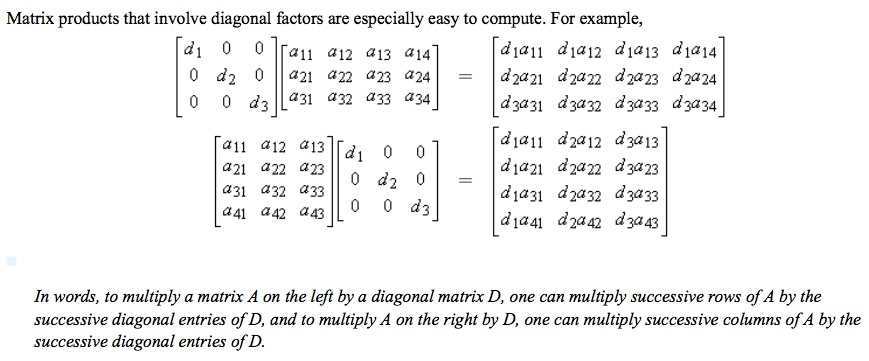
\includegraphics[scale=0.55]{figures_mvc/Mult_by_Diagonal_Matrix}

\begin{exercise}
Let $A=\begin{bmatrix}
	3 & 0 & 0 \\ 0 & 2 & 0 \\ 0 & 0 & 5
\end{bmatrix}, B=\begin{bmatrix}
	-1 & 2 & 0 \\ 5 & 3 & 4 \\ 
\end{bmatrix}, C=\begin{bmatrix}
	5 & 1 & -2 & 3 \\ 1 & 1 & -1 & 0 \\ 
	6 & 2 & 3 & -4
\end{bmatrix}$. Compute $BA$ and $AC$.
\end{exercise}

\subsubsection{Triangular matrices}
	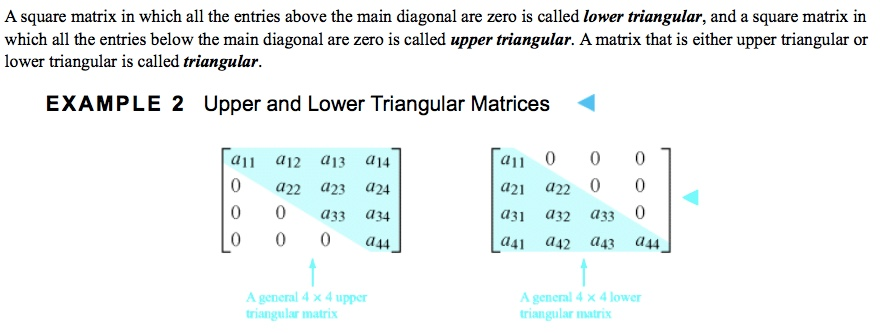
\includegraphics[scale=0.55]{figures_mvc/Triangular_Matrices} 
	
In terms of the matrix elements $a_{ij}$: 
\begin{itemize}
	\item A square matrix is lower triangular if $a_{ij}=0$ for $i<j$.
	\item A square matrix is upper triangular if $a_{ij}=0$ for $i>j$.
\end{itemize}

\begin{thm}[Properties of triangular matrices] \label{thm:properties_of_triangular_matrices} \hspace{10cm}
		\begin{enumerate}[(a)]
	\item If $A$ is lower (upper) triangular, then $A^T$ is upper (lower) triangular.
	\item If $A_1,\cdots, A_k$ are lower (upper) triangular, then so is the product $A_1\cdots A_k$.
	\item A triangular matrix is invertible if and only if its diagonal entries are all nonzero.
	\item If $A$ is an invertible lower (upper) triangular matrix, then so is $A^{-1}$.
	\end{enumerate}
\end{thm}

\begin{pf}
(a) $A$ lower triangular means $a_{ij}=0$ for $i<j$. Since $(A^T)_{ij}=a_{ji}$, $(A^T)_{ij}=0$ for $i>j$, hence $A^T$ is upper triangular. 

(b) Suppose $A$ and $B$ are lower triangular. Then 
\begin{align*}
	(AB)_{ij}=\sum_{k=1}^{n}A_{ik}B_{kj}=\sum_{k=1}^{j-1}A_{ik}\underbrace{B_{kj}}_{=0 \ \forall k}+\sum_{k=j}^{n}\underbrace{A_{ik}}_{=0 \ \forall k}B_{kj}=0.
\end{align*}
The fact that $A_1 A_2 \cdots A_k$ is lower (upper) triangular if $A_1, A_2,\cdots, A_k$ are follows by induction on $k$. 

(c) If $d_j=0$ for some $j$, then the $j$th column would not be a pivot column, so $A$ would not be row-equivalent to $I$ and hence would not be invertible. 

(d) We will prove this later once we have a formula for $A^{-1}$ for a general $n \times n$ invertible matrix.	
\end{pf}

\begin{exercise}
Let $A=\begin{bmatrix}
		1 & 3 & -1 \\ 0 & 2 & 4 \\ 0 & 0 & 5
	\end{bmatrix}, B= \begin{bmatrix}
		3 & -2 & 2 \\ 0 & 0 & -1 \\ 0 & 0 & 1
	\end{bmatrix}$. Compute $A^{-1}, B^{-1}, AB,$ and $BA$.	
\end{exercise}

\subsubsection{Symmetric matrices}
A square matrix $A$ is {\bf symmetric} if $A=A^T$. Some examples are
\begin{align*}
	\begin{bmatrix}
		7 & -3 \\ -3 & 5
	\end{bmatrix}, \begin{bmatrix}
		1 & 4 & 5 \\ 4 & -3 & 0 \\ 5 & 0 & 7
	\end{bmatrix}, \begin{bmatrix}
		d_1 & 0 & 0 & 0 \\ 0 & d_2 & 0 & 0 \\ 0 & 0 & d_3 & 0 \\ 0 & 0 & 0 & d_4
	\end{bmatrix}
\end{align*}
In terms of the matrix elements $a_{ij}$, a matrix is symmetric if $a_{ij}=a_{ji}$ for all $i,j$.
 
\begin{thm}[Properties of symmetric matrices]
		If $A$ and $B$ are symmetric matrices with the same size, and if $k$ is any scalar, then
\begin{enumerate}[(a)] 
	\item $A^T$ is symmetric.
	\item $A+B$ and $A-B$ are symmetric.
	\item $kA$ is symmetric.
	\item If $A$ and $B$ are symmetric, then $AB$ is symmetric if and only if $A$ and $B$ commute.
	\item If $A$ is an invertible symmetric matrix, then $A^{-1}$ is symmetric.
\end{enumerate}
\end{thm}

\begin{pf}
(a) $(A^T)^T=A=A^T$ (since $A$ is symmetric), hence $A^T$ is symmetric. 

(b) $(A+B)^T=A^T+B^T=A+B$.

(c) $(kA)^T=kA^T=kA$. 

(d) $(AB)^T=B^TA^T=BA$. Then $BA=AB \iff A$ and $B$ commute. 

(e) We will prove this later once we have a formula for $A^{-1}$ for a general invertible matrix.
\end{pf}

\subsubsection{$AA^T$ and $A^TA$}
Matrix products of the form $AA^T$ and $A^TA$ arise in a variety of applications. 

\begin{thm}[Properties of $AA^T$ and $A^TA$]\label{thm:props_of_aat_and_ata}
	\begin{enumerate}[(a)]
		\item The products $AA^T$ and $A^TA$ are both square matrices. They are the same size if and only if $A$ is a square matrix.
		\item The products $AA^T$ and $A^TA$ are both symmetric.
		\item If $A$ is invertible, then $AA^T$ and $A^TA$ are also invertible.
	\end{enumerate}
\end{thm}

\begin{pf}
	\begin{enumerate}[(a)]
		\item If $A$ is $m\times n$, $A^T$ is $n \times m$. Therefore $AA^T$ is $m \times m$ and $A^TA$ is $n \times n$. They are the same size iff $n=m$, i.e., if $A$ is a square matrix.
		\item $(AA^T)^T=(A^T)^T(A)^T=AA^T$. $(A^TA)^T=(A)^T(A^T)^T=A^TA$.
		\item $(AA^T)^{-1}=(A^T)^{-1}A^{-1}=(A^{-1})^TA^{-1}$. $(A^TA)^{-1}=A^{-1}(A^T)^{-1}=A^{-1}(A^{-1})^T$.
	\end{enumerate}
\end{pf}

\begin{exercise}
	Let $A=\begin{bmatrix}
		1 & -2 & 4 \\ 3 & 0 & -5
	\end{bmatrix}$. Show explicitly that $A^TA$ and $AA^T$ are symmetric matrices.	
\end{exercise}

\section{Determinants}\label{sec:determinants}
\subsection{Condition for invertibility}
We have seen that not all $n \times n$ matrices have an inverse. We would now like to ask, given an arbitrary $n \times n$ matrix $A$, what is the set of conditions on the entries of $A$ which are both necessary and sufficient for $A$ to be invertible?

In the case of a $1 \times 1$ matrix
\begin{align*}
	A=\begin{bmatrix}
		a
	\end{bmatrix},
\end{align*}
we see immediately that $A$ is invertible if and only if $a \neq 0$.

Consider now a general $2 \times 2$ matrix
\begin{align*}
	A=\begin{bmatrix}
		a_{11} & a_{12} \\
		a_{21} & a_{22}
	\end{bmatrix}.
\end{align*}
If the first column of $A$ is zero, then $A$ is not invertible, so the first column of $A$ must have at least one nonzero entry. Interchanging the two rows if necessary, without loss of generality we may assume that $a_{11} \neq 0$. If $a_{21}=0$, then $A$ is of the form
\begin{align*}
	\begin{bmatrix}
		a_{11} & a_{12} \\
		0 & a_{22}
	\end{bmatrix}
\end{align*}
and is therefore invertible if and only if $a_{22} \neq 0$, in which case the second column will also be a pivot column.

If $a_{21}\neq 0$, then perform the following sequence of elementary row operations:
\begin{align*}
	\begin{bmatrix}
		a_{11} & a_{12}  \\
		a_{21} & a_{22}  
	\end{bmatrix} \stackrel{\stackrel{R1 \mapsto a_{21}R1}{R2 \mapsto a_{11}R2}}{\longrightarrow} \begin{bmatrix}
		a_{11}a_{21} & a_{12}a_{21}  \\
		a_{11}a_{21} & a_{11}a_{22} 
	\end{bmatrix} \stackrel{R2 \mapsto R2-R1}{\longrightarrow} \begin{bmatrix}
		a_{11}a_{21} & a_{12}a_{21}\\
		0 & a_{11}a_{22}-a_{12}a_{21}
	\end{bmatrix}.
\end{align*}
Since $a_{11}a_{21} \neq 0$ by assumption, the first column is a pivot column. The second column is a pivot column if and only if the quantity $a_{11}a_{22}-a_{21}a_{12} \neq 0$. Note that the quantity $a_{11}a_{22}-a_{21}a_{12}$ is zero if any row or column of $A$ is zero, so the \emph{single} condition $a_{11}a_{22}-a_{21}a_{12} \neq 0$ is actually both necessary \emph{and sufficient} for $A$ to be invertible.

Let $|A|\equiv a_{11}a_{22}-a_{21}a_{12}$. Assuming $|A| \neq 0$, we can continue to sequence of elementary row operations above on the augmented matrix $[A|I]$ to obtain a general formula for $A^{-1}$:
\begin{align*}
	\begin{bmatrix}
		a_{11} & a_{12} & \aug & 1 & 0 \\
		a_{21} & a_{22} & \aug & 0 & 1 
	\end{bmatrix} \stackrel{\stackrel{R1 \mapsto a_{21}R1}{R2 \mapsto a_{11}R2}}{\longrightarrow} \begin{bmatrix}
		a_{11}a_{21} & a_{12}a_{21} & \aug & a_{21} & 0 \\
		a_{11}a_{21} & a_{11}a_{22} & \aug & 0 & a_{11}
	\end{bmatrix} \stackrel{R2 \mapsto R2-R1}{\longrightarrow} \begin{bmatrix}
		a_{11}a_{21} & a_{12}a_{21} & \aug & a_{21} & 0 \\
		0 & a_{11}a_{22}-a_{12}a_{21} & \aug & -a_{21} & a_{11}
	\end{bmatrix} \\
	\stackrel{R2 \mapsto \frac{1}{|A|}R2}{\longrightarrow}\begin{bmatrix}
		a_{11}a_{21} & a_{12}a_{21} & \aug & a_{21} & 0 \\
		0 & 1 & \aug & -\frac{a_{21}}{|A|} & \frac{a_{11}}{|A|}
	\end{bmatrix} \stackrel{R1 \mapsto -a_{12}a_{21}R2+R1}{\longrightarrow} \begin{bmatrix}
		a_{11}a_{21} & 0 & \aug & a_{21}+\frac{a_{12}a_{21}^2}{|A|} & -\frac{a_{11}a_{12}a_{21}}{|A|} \\
		0 & 1 & \aug & -\frac{a_{21}}{|A|} & \frac{a_{11}}{|A|} \end{bmatrix} \\
		\stackrel{R1 \mapsto \frac{1}{a_{11}a_{21}}R1}{\longrightarrow}
	 \begin{bmatrix}
		1 & 0 & \aug & \frac{a_{21}}{a_{11}a_{21}}+\frac{a_{12}a_{21}^2}{a_{11}a_{21}|A|} & -\frac{a_{11}a_{12}a_{21}}{a_{11}a_{21}|A|} \\
		0 & 1 & \aug & -\frac{a_{21}}{|A|} & \frac{a_{11}}{|A|} 
	\end{bmatrix}= \begin{bmatrix}
		1 & 0 & \aug & \frac{a_{21}|A|}{a_{11}a_{21}|A|}+\frac{a_{12}a_{21}^2}{a_{11}a_{21}|A|} & -\frac{a_{12}}{|A|} \\
		0 & 1 & \aug & -\frac{a_{21}}{|A|} & \frac{a_{11}}{|A|} 
	\end{bmatrix} \\
	=\begin{bmatrix}
		1 & 0 & \aug & \frac{a_{21}(a_{11}a_{22}-a_{12}a_{21})}{a_{11}a_{21}|A|}+\frac{a_{12}a_{21}^2}{a_{11}a_{21}|A|} & -\frac{a_{12}}{|A|} \\
		0 & 1 & \aug & -\frac{a_{21}}{|A|} & \frac{a_{11}}{|A|} 
	\end{bmatrix}=\begin{bmatrix}
		1 & 0 & \aug & \frac{a_{21}(a_{11}a_{22}-a_{12}a_{21})+a_{12}a_{21}^2}{a_{11}a_{21}|A|} & -\frac{a_{12}}{|A|} \\
		0 & 1 & \aug & -\frac{a_{21}}{|A|} & \frac{a_{11}}{|A|} 
	\end{bmatrix} \\
	=\begin{bmatrix}
		1 & 0 & \aug & \frac{a_{21}a_{11}a_{22}-a_{12}a_{21}^2+a_{12}a_{21}^2}{a_{11}a_{21}|A|} & -\frac{a_{12}}{|A|} \\
		0 & 1 & \aug & -\frac{a_{21}}{|A|} & \frac{a_{11}}{|A|} 
	\end{bmatrix}=\begin{bmatrix}
		1 & 0 & \aug & \frac{a_{21}a_{11}a_{22}}{a_{11}a_{21}|A|} & -\frac{a_{12}}{|A|} \\
		0 & 1 & \aug & -\frac{a_{21}}{|A|} & \frac{a_{11}}{|A|} 
	\end{bmatrix}=\begin{bmatrix}
		1 & 0 & \aug & \frac{a_{22}}{|A|} & -\frac{a_{12}}{|A|} \\
		0 & 1 & \aug & -\frac{a_{21}}{|A|} & \frac{a_{11}}{|A|} 
	\end{bmatrix}
\end{align*}
We have therefore proved the following:
\begin{prop}[Formula for inverse of a $2 \times 2$ matrix]
A $2 \times 2$ matrix 
\begin{align*}
	A=\begin{bmatrix}
		a_{11} & a_{12} \\
		a_{21} & a_{22}
	\end{bmatrix}
\end{align*}
is invertible if and only if $|A|=a_{11}a_{22}a_{12}a_{21} \neq 0$, in which case $A^{-1}$ is given by the formula
\begin{align*}
	A^{-1}=\frac{1}{|A|}\begin{bmatrix}
		a_{22} & -a_{12} \\
		-a_{21} & a_{11}
	\end{bmatrix}.
\end{align*}	
\end{prop}

\begin{exercise}
	Consider a general $3 \times 3$ matrix
\begin{align*}
	A=\begin{bmatrix}
		a_{11} & a_{12} & a_{13} \\
		a_{21} & a_{22} & a_{23} \\
		a_{31} & a_{32} & a_{33}
	\end{bmatrix}.
\end{align*}
For $A$ to be invertible, the first column must have a nonzero entry. By exchanging rows, if necessary, we may assume without loss of generality that $a_{11} \neq 0$.
\begin{enumerate}[(a)]
	\item Perform a sequence of elementary row operations to put $A$ into the row-equivalent form
	\begin{align*}
		\begin{bmatrix}
		a_{11} & a_{12} & a_{13} \\
		0 & a_{11}a_{22}-a_{12}a_{21} & a_{11}a_{23} - a_{13}a_{21} \\
		0 & a_{11}a_{32}-a_{12}a_{31} & a_{11}a_{33}-a_{13}a_{31}
	\end{bmatrix}.
	\end{align*}
	\item For $A$ to be invertible, the second column must be a pivot column. Without loss of generality, we may assume the $(2,2)$-entry is nonzero. Continue performing elementary row operations to show that $A$ can be put in the row-equivalent form
	\begin{align*}
		\begin{bmatrix}
			a_{11} & a_{12} & a_{13} \\
			0 & a_{11}a_{22}-a_{12}a_{21} & a_{11}a_{23}-a_{13}a_{21} \\
			0 & 0 & a_{11}|A|
		\end{bmatrix}
	\end{align*}
	where now $|A|$ is given by 
	\begin{align*}
		|A|\equiv a_{11}(a_{22}a_{33}-a_{23}a_{32})-a_{12}(a_{21}a_{33}-a_{23}a_{31})+a_{13}(a_{21}a_{32}-a_{22}a_{31}).
	\end{align*}
	Conclude that the single condition $|A| \neq 0$ is both necessary and condition for $A$ to be invertible.
\end{enumerate}
\end{exercise}

We have just seen that for a $1 \times 1$, $2 \times 2$, or $3 \times 3$ matrix $A$, invertibility of $A$ is determined by a single number, $|A|$. We call this number the \emph{determinant} of the matrix $A$, which is also denoted $\det A$. \footnote{Note that the notation $|A|$ has nothing to do with absolute value.}

Looking at the determinant formulas for each case above, we notice that these can be written in the following recursive fashion:
\begin{align}
	\begin{vmatrix}
	a_{11}	
	\end{vmatrix} &=a_{11} \\
	\begin{vmatrix}
		a_{11} & a_{12} \\ a_{21} & a_{22}
	\end{vmatrix} &=a_{11}a_{22}-a_{12}a_{21} \label{eq:2_by_2_det} \\
	&=a_{11}|a_{22}|-a_{12}|a_{21}|, \\
	\begin{vmatrix}
		a_{11} & a_{12} & a_{13} \\ a_{21} & a_{22} & a_{23} \\ a_{31} & a_{32} & a_{33}
	\end{vmatrix}&=a_{11}(a_{22}a_{33}-a_{23}a_{32})-a_{12}(a_{21}a_{33}-a_{23}a_{31})+a_{13}(a_{21}a_{32}-a_{22}a_{31}) \\
	&=a_{11}\begin{vmatrix}
		a_{22} & a_{23} \\ a_{32} & a_{33}
	\end{vmatrix}-a_{12}\begin{vmatrix}
		a_{21} & a_{23} \\ a_{31} & a_{33}
	\end{vmatrix}+a_{13} \begin{vmatrix}
		a_{21} & a_{22} \\ a_{31} & a_{32}
	\end{vmatrix}.
\end{align}

We can use this to recursively define the determinant of an $n \times n$ matrix.

\begin{defn}[Determinant of an $n \times n$ matrix]
	Let $A$ be an $n \times n$ matrix, and let $A_{ij}$ denote the $(n-1) \times (n-1)$ submatrix of $A$ obtained by deleting the $i$th row and $j$th column of $A$. Define the $(i,j)$-\emph{cofactor} of $A$ to be the number $C_{ij}=(-1)^{i+j}\det A_{ij}$. \footnote{The determinant $\det A_{ij}$ is called the $(i,j)$ \emph{minor determinant} of $A$.} We then define the determinant of $A$ to be the number
	\begin{align}\label{eq:cof_along_first_row}
		\det A=\sum_{j=1}^n a_{1j}C_{1j}.
	\end{align}
	This formula is said to be a \emph{cofactor expansion} along the first row of $A$.
\end{defn}

It remains to be shown that an $n \times n$ matrix $A$ is invertible if and only if $\det A \neq 0$ when $n>3$. This will be done in Section \ref{sec:cramer}. Therefore, we have added yet another equivalent condition to the Invertible Matrix Theorem:

\begin{thm}[Invertible matrix theorem]\label{thm:invertible_matrix_theorem_part_3}
	If $A$ is an $n \times n$ matrix, the following are equivalent.
	\begin{enumerate}[(i)]
		\item $A$ is invertible.
		\item $A$ is row-equivalent to the $n \times n$ identity matrix.
		\item $A$ is a product of elementary matrices.
		\item The linear system $A\mathbf{x}=\mathbf{b}$ has a unique solution.
		\item $\det A \neq 0$.
	\end{enumerate} 	
\end{thm}


\begin{exercise}
Show that the formula for the determinant of a $2 \times 2$ and $3 \times 3$ matrix are given by the formula in Equation \eqref{eq:cof_along_first_row}.
\end{exercise}

\begin{exercise}
Let $A=\begin{bmatrix}
	3 & 1 & -4 \\ 2 & 5 & 6 \\ 1 & 4 & 8
\end{bmatrix}$. 
\begin{enumerate}[(a)]
	\item Compute the $(1,1)$ and $(1,2)$ minor determinants and cofactors of $A$.
	\item Compute the determinant of $A$.
\end{enumerate}	
\end{exercise}

Let us now consider again our $n \times n$ matrix $A$ to be the coefficient matrix of a system of linear equations. The Invertible Matrix Theorem (\ref{thm:invertible_matrix_theorem_part_3}) tells us that the system has a unique solution if and only if $A$ is invertible, that is, if and only if $\det A=0$. The solution set of our system of course does not depend on the order in which we list the equations. However, the formula
\begin{align*}
	\det A=\sum_{j=1}^na_{1j}C_{1j}
\end{align*}
singles out the first row of our matrix $A$ as special. This choice is immaterial, and only reflects one possible convention for the steps in the Gauss-Jordan elimination algorithm. Similarly, our ordering of the variables was also merely a choice, and could have been chosen differently (e.g., could have chosen the first column of the matrix to correspond to $x_5$ rather than $x_1$, etc.) Hence, we have the following theorem
\begin{thm}[Cofactor expansion along any row or column]
	The determinant of an $n \times n$ matrix $A$ can be computed by cofactor expansion along any row or column. The cofactor expansion across the $i$th row is given by
	\begin{align*}
		\det A=\sum_{j=1}^na_{ij}C_{ij}
	\end{align*}
	and the cofactor expansion down the $j$th column is given by
	\begin{align*}
		\det A=\sum_{i=1}^na_{ij}C_{ij}.
	\end{align*}
\end{thm}

\begin{exercise}
Compute the determinant of the matrix
\begin{align*}
	A=\begin{bmatrix}
		1 & 5 & 0 \\
		2 & 4 & -1 \\
		0 & -2 & 0
	\end{bmatrix}
\end{align*}
	by cofactor expansion along
	\begin{enumerate}[(a)]
		\item The second row.
		\item The third row.
		\item The third column.
	\end{enumerate}	
\end{exercise}

\begin{exercise}
Consider the sign $(-1)^{i+j}$ appearing in the $(i,j)$-cofactor $C_{ij}$ as an $n \times n$ matrix. Work out the entries for $n=2,3,4$. What do you notice? How can this help you work out the signs of the cofactors quickly when you are computing a determinant?	
\end{exercise}

\begin{exercise}
Compute the determinant of the matrix
\begin{align*}
	A=\begin{bmatrix}
		3 & -7 & 8 & 9 & -6 \\
		0 & 2 & -5 & 7 & 3 \\
		0 & 0 & 1 & 5 & 0 \\
		0 & 0 & 2 & 4 & -1 \\
		0 & 0 & 0 & -2 & 0
	\end{bmatrix}.
\end{align*}
\emph{Hint: Compute $\det A$ by cofactor expansion along the first column. Why is this the best choice?}	
\end{exercise}

\begin{exercise}
We have argued previously that an $n \times n$ matrix with a row or column of zeros is not invertible. What is the determinant of a matrix a row or column of zeros?	
\end{exercise}

\begin{exercise}
Compute the determinant of each of the following matrices:
\begin{align*}
	A=\begin{bmatrix}
		2 & 0 & 0 \\
		0 & -1 & 0 \\
		0 & 0 & 3
	\end{bmatrix}, \hspace{0.5cm} B=\begin{bmatrix}
		2 & 0 & 0 \\
		0 & 0 & 0 \\
		0 & 0 & 3
	\end{bmatrix}.
\end{align*}	
\end{exercise}

\begin{thm}[Determinant of a diagonal matrix]\label{thm:determinant_of_a_diagonal_matrix}
	Let $D$ be a diagonal $n \times n$ matrix and let $d_{ii}$ denote the $(i,i)$-entry of $A$. Then $\det D=\prod_{i=1}^n d_{ii}$.
\end{thm}

\begin{proof}
	(By induction on $n$.) For a $2 \times 2$ diagonal matrix $D=\begin{bmatrix}
		d_{11} & 0 \\
		0 & d_{22}
	\end{bmatrix}$, the formula in Equation \eqref{eq:2_by_2_det} gives $\det D=d_{11}d_{22}$. Suppose now that the proposition is true for a $(k-1) \times (k-1)$ diagonal matrix and consider a $k \times k$ diagonal matrix
	\begin{align*}
		D=\begin{bmatrix}
			d_{11} & 0 & 0 & \cdots & 0 \\
			0 & d_{22} & 0 & \cdots & 0 \\
			0 & 0 & d_{33} & \cdots & 0 \\
			\vdots & \vdots & \vdots & \ddots & \vdots \\
			0 & 0 & 0 & \cdots & d_{kk}
		\end{bmatrix}.
	\end{align*}
	Computing $\det D$ by cofactor expansion along the first row, gives 
	\begin{align*}
		\det D=d_{11}\begin{vmatrix}
			d_{22} & 0 & 0 & \cdots & 0 \\
			0 & d_{33} & 0 & \cdots & 0 \\
			0 & 0 & d_{44} & \cdots & 0 \\
			\vdots & \vdots & \vdots & \ddots & \vdots \\
			0 & 0 & 0 & \cdots & d_{kk}
		\end{vmatrix}
	\end{align*}.
	Since $\begin{bmatrix}
			d_{22} & 0 & 0 & \cdots & 0 \\
			0 & d_{33} & 0 & \cdots & 0 \\
			0 & 0 & d_{44} & \cdots & 0 \\
			\vdots & \vdots & \vdots & \ddots & \vdots \\
			0 & 0 & 0 & \cdots & d_{kk}
		\end{bmatrix}$ is a $(k-1) \times (k-1)$ matrix, by the inductive hypothesis we have  $\begin{vmatrix}
			d_{22} & 0 & 0 & \cdots & 0 \\
			0 & d_{33} & 0 & \cdots & 0 \\
			0 & 0 & d_{44} & \cdots & 0 \\
			\vdots & \vdots & \vdots & \ddots & \vdots \\
			0 & 0 & 0 & \cdots & d_{kk}
		\end{vmatrix}=\prod_{i=2}^kd_{ii}$ and therefore $\det D=\prod_{i=1}^kd_{ii}$, as desired.
\end{proof}

\begin{cor}[Invertibility of a diagonal matrix]\label{cor:invertibility_of_a_diagonal_matrix}
	A diagonal matrix is invertible if and only if each element on the main diagonal is nonzero.
\end{cor}

\begin{exercise}
Prove Corollary	\ref{cor:invertibility_of_a_diagonal_matrix}.
\end{exercise}

\begin{exercise}
Compute the determinant of each of the following matrices:
\begin{align*}
	A=\begin{bmatrix}
		1 & -1 & 2 & 4 \\
		0 & 2 & 4 & -5 \\
		0 & 0 & 1 & 2 \\
		0 & 0 & 0 & 3
	\end{bmatrix}, \hspace{0.5cm} B=\begin{bmatrix}
		1 & -1 & 2 & 4 \\
		0 & 2 & 4 & -5 \\
		0 & 0 & 0 & 2 \\
		0 & 0 & 0 & 3
	\end{bmatrix}.
\end{align*}	
\end{exercise}

\begin{thm}[Determinant of a triangular matrix]\label{thm:determinant_of_a_triangular_matrix}
	Let $T$ be an $n \times n$ triangular matrix. Let $d_{ii}$ denote the diagonal entries of $T$. Then $\det T=\prod_{i=1}^n d_{ii}$.
\end{thm}

\begin{exercise}
	Prove Theorem \ref{thm:determinant_of_a_triangular_matrix} by induction. \emph{Hint:} Copy the steps in the proof of Theorem \ref{thm:determinant_of_a_diagonal_matrix}.
\end{exercise}

\begin{cor}[Invertibility of a triangular matrix]
	A triangular matrix is invertible if and only if each element on the main diagonal is nonzero.
\end{cor}

\begin{exercise}
Let $A=\begin{bmatrix}
	3 & 0 & 0 \\
	2 & -1 & 0 \\
	1 & 9 & -4
\end{bmatrix}$. Compute $\det A$ and $\det A^T$. What do you notice?	
\end{exercise}

\begin{thm}[Determinant of a Transpose]\label{thm:determinant_of_a_transpose}
	For any $n \times n$ matrix, $\det A^T=\det A$.
\end{thm}

\begin{proof}
We prove the theorem by induction on $n$. The theorem holds trivially for $n=1$ and is easily verified for $n=2$. Suppose now that the theorem holds for $n=k$. Let $A$ be a $(k+1) \times (k+1)$ matrix. Computing the determinant of $A^T$ along the first row gives
\begin{align*}
	\det A^T=\sum_{i=1}^n(a^T)_{1i}C_{1i}
\end{align*}
where $C_{1i}=(-1)^{1+i}\det A^T_{1i}$. Noting that $A^T_{1i}=(A_{i1})^T$, \footnote{This can be seen by thinking through the definitions of each side. To help with this, consider a $3 \times 3$ matrix $A=\begin{bmatrix}
	a_{11} & a_{12} & a_{13} \\
	a_{21} & a_{22} & a_{23} \\
	a_{31} & a_{32} & a_{33}
\end{bmatrix}$. Then $A^T=\begin{bmatrix}
	a_{11} & a_{21} & a_{31} \\
	a_{12} & a_{22} & a_{32} \\
	a_{13} & a_{23} & a_{33}
\end{bmatrix}$. Taking $i=3$, we have $(A^T)_{31}=\begin{bmatrix}
	a_{21} & a_{31} \\
	a_{22} & a_{32}
\end{bmatrix}$. On the other hand, $A_{13}=\begin{bmatrix}
	a_{21} & a_{22} \\
	a_{31} & a_{32}
\end{bmatrix}$, which is the transpose of $(A^T)_{31}$, so indeed $(A^T)_{31}=(A_{31})^T$.} we therefore have
\begin{align*}
	\det A^T=\sum_{i=1}^n(a^T)_{1i}(-1)^{1+i}\det (A_{i1})^T
\end{align*} 
Since $(A_{i1})^T$ is a $k \times k$ matrix, by the inductive hypothesis we have $\det (A_{i1})^T= \det A_{i1}$. Since we also have $(a^T)_{1i}=a_{i1}$, we find
\begin{align*}
	\det A^T&=\sum_{i=1}^n(a^T)_{1i}C_{1i} \\
	&=\sum_{i=1}^n(a^T)_{1i}(-1)^{1+i}\det A^T_{1i} \\
	&=\sum_{i=1}^n(a^T)_{1i}(-1)^{1+i}\det (A_{i1})^T \\
	&=\sum_{i=1}^na_{i1}(-1)^{i+1}\det A_{i1}
\end{align*} 
which is the cofactor expansion of $\det A$ along the first \emph{column}. Since the determinant of $A$ can be computed by cofactor expansion along any row or column, we have shown that $\det A^T=\det A$, as desired. 
\end{proof}

\subsection{Row Operations and Determinants}
In the previous section, we saw that the determinant of an $n \times n$ matrix $A$ can be computed by cofactor expansion by the formula
\begin{align*}
	\det A=\sum_{j=1}^na_{ij}C_{ij}
\end{align*}
across any row or column. By choosing a row or column with many zero entries, the computation of the determinant is greatly simplified. However, for a matrix which has no zero entries, the computation quickly becomes very tedious, as cofactor expansion requires $\mathcal{O}(n!)$ operations. To see how quickly the complexity of the computation grows, for $n=25$, $n!\cong 1.5 \times 10^{25}$. A computer performing $10^{12}$ operations per second would take 500,000 years to compute the determinant of a $25 \times 25$ matrix by this method! By today's standards, a $25 \times 25$ matrix is \emph{very small}, so we clearly need a more practical way to compute determinants.

It was proved in Theorem \ref{thm:determinant_of_a_triangular_matrix} that the determinant of a triangular $n \times n$ matrix $T$ requires only $n$ multiplications, since the determinant is simply the product of the diagonal entries of $T$. Since any row-echelon form, $U$, of an $n \times n$ matrix $A$ is an upper triangular matrix, a strategy to compute the determinant of $A$ efficiently would be to row-reduce $A$ to $U$, and then compute the determinant of $U$. To do so, we will need to know how $\det U$ is related to $\det A$.

\begin{exercise}
Consider a general $3 \times 3$ matrix
\begin{align*}
	A=\begin{bmatrix}
		a_{11} & a_{12} & a_{13} \\
		a_{21} & a_{22} & a_{23} \\
		a_{31} & a_{32} & a_{33}
	\end{bmatrix}. 
\end{align*}	
Let $B$ be a matrix row-equivalent to $A$ by the following elementary row operations. In each case, compute $\det B$ and compare it to $\det A$.
\begin{enumerate}[(a)]
	\item $R1 \mapsto c R_1, c \neq 0$.
	\item $R1 \leftrightarrow R2$.
	\item $R1 \mapsto R1+cR2$.
\end{enumerate}
\end{exercise}

\begin{thm}[Elementary row operations and determinants]
	Let $A$ be an $n \times n$ matrix. Then
	\begin{enumerate}[(a)]
		\item Row replacements do not change $\det A$.
		\item Each interchange changes the sign of $\det A$.
		\item Multiplying a row by $c$ multiplies $\det A$ by $c$.
	\end{enumerate}
	\begin{center}
		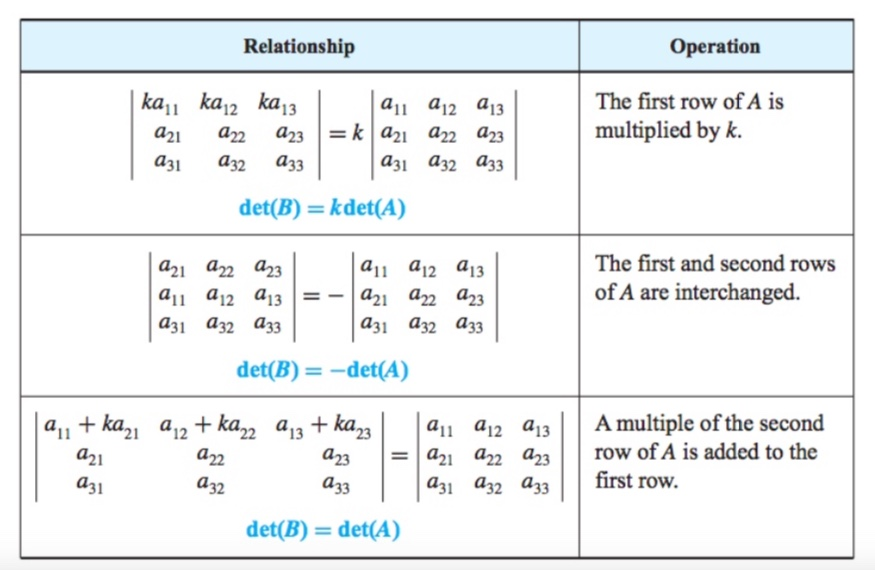
\includegraphics[scale=0.4]{figures_mvc/ero_and_det}
	\end{center}
\end{thm}
To prove this theorem, it will be useful to rephrase it in terms of elementary matrices, as follows.
\begin{thm}[Elementary matrices and determinants]\label{thm:elementary_matrices_and_determinants}
	If $A$ is an $n \times n$ matrix and $E$ is an $n \times n$ elementary matrix, then
	\begin{align*}
		\det EA=(\det E)(\det A)
	\end{align*}
	where
	\begin{align*}
		\det E=\begin{cases}
			&1 \text{ if $E$ is a row-replacement}, \\
			&-1 \text{ if $E$ is an interchange}, \\
			&c \text{ if $E$ is scaling by $c$}.
		\end{cases}
	\end{align*}
\end{thm}

\begin{proof}
(By induction on $n$.) Using the list of $2 \times 2$ elementary matrices from Exercise \ref{ex:2_by_2_elementary_matrices}, we check that the determinant of each is indeed equal to $1,-1,$ or $c$, depending on the elementary row-operation. Taking a general $2 \times 2$ matrix $A=\begin{bmatrix}
	a & b \\ c & d
\end{bmatrix}$, we now check that the theorem holds in each case. For instance, if $E=\begin{bmatrix}
	1 & 0 \\ k & 1
\end{bmatrix}$, then we have
\begin{align*}
	\det EA&=\begin{vmatrix}
		a+kc & b+kd \\
		c & d
	\end{vmatrix} \\
	&=(a+kc)d-c(b+kd) \\
	&=ad+kcd-cb-ckd \\
	&=ad-bc \\
	&=\det A.
\end{align*} 
This establishes the base case. Now suppose the theorem holds for $n=k$ and let $A$ be a $k \times k$ matrix. Expand $\det EA$ along a row which is unaffected by $E$, say row $i$:
\begin{align*}
	det EA=\sum_{j=1}^{k+1}a_{ij}(-1)^{i+j}\det (EA)_{ij}.
\end{align*}
Since the matrix $(EA)_{ij}$ is $k \times k$, by the inductive hypothesis $\det (EA)_{ij}=\alpha \det A_{ij}$, where $\alpha =1,-1,$ or $c$, depending on $E$. Thus
\begin{align*}
	\det EA &=\sum_{j=1}^{k+1}a_{ij}(-1)^{i+j}\det (EA)_{ij} \\
	&=\sum_{j=1}^{k+1}a_{ij}(-1)^{i+j}(\alpha\det A_{ij}) \\
	&=\alpha\sum_{j=1}^{k+1}a_{ij}(-1)^{i+j}\det A_{ij} \\
	&=\alpha \det A,
\end{align*}
proving the theorem. In particular, taking $A=I$ to be the $n \times n$ identity matrix, we see that $\det E=1,-1$, or $c$, depending on $E$.
\end{proof}

Suppose now that an $n \times n$ matrix $A$ has been reduced to a row-echelon form $U$ by $r$ interchanges and any number of row-replacements. \footnote{Note that we do not need to scale any of the rows, since we only need to reduce $U$ to any REF, and not RREF.} Since $U$ is triangular, $\det U=\prod_{i=1}^n u_{ii}$ is the product of its diagonal entries $u_{ii}$. If $A$ is invertible, then each of these is nonzero. Otherwise, at lease one of the $u_{ii}$ is zero. Since we can write $U=PA$, where $P$ is a product of elementary matrices corresponding to the elementary row operations taking $A$ to $U$, by Theorem \ref{thm:elementary_matrices_and_determinants} we have

\begin{cor}[Determinant of a matrix by row operations]\label{cor:determinant_of_a_matrix_by_row_operations}
	Let $A$ be an $n \times n$ matrix which has been reduced to a row-echelon form $U$ by $r$ interchanges and any number of row-replacements. Then 
	\begin{align*}
		\det A=\begin{cases}
			(-1)^r\prod_{i=1}^nu_{ii} \hspace{0.5cm}\text{ (if $A$ is invertible)}, \\
			0 \hspace{2.7cm} \text{ (if $A$ is not invertible)},
		\end{cases}
	\end{align*}
	where $\prod_{i=1}^nu_{ii}=\det U$.
\end{cor}

\fixme{Need to prove that, while $U$ is not unique, $\det U$ is. Or is this obvious?}

\begin{cor}[Invertibility condition]
	An $n \times n$ matrix $A$ is invertible if and only if $\det A \neq 0$.
\end{cor}

Most computers use the method of \ref{cor:determinant_of_a_matrix_by_row_operations} to compute $\det A$: when $A$ is $n \times n$, it can be shown that the computation of $\det A$ by row operations requires only $\mathcal{O}(n^3)$ operations. For $n=25$, this is only about 15,000 operations, which any modern computer can carry out in a fraction of a second.

\begin{exercise}
Use row-reduction to compute the determinant of 
\begin{align*}
	A=\begin{bmatrix}
		1 & -4 & 2 \\
		-2 & 8 & -9 \\
		-1 & 7 & 0
	\end{bmatrix}.
\end{align*}	
\end{exercise}

\begin{prop}[Matrices with proportional rows or columns]
	If an $n \times n$ matrix $A$ has two rows or columns that are scalar multiples of each other, then $\det A=0$.
\end{prop}

\begin{proof}
	If $A$ has two proportional rows, then by a row replacement it has a row of zeros and therefore $\det A=0$. If $A$ has two columns which are proportional, then $A^T$ has two rows which are proportional. By the same comments above applied to $A^T$, $\det A^T=0$. Since $\det A^T=\det A$ (by Theorem \ref{thm:determinant_of_a_transpose}), $\det A=0$, completing the proof. 
\end{proof}

\subsection{Properties of Determinants}

\begin{exercise}
Let $A=\begin{bmatrix}
	6 & 1 \\ 3 & 2
\end{bmatrix}$ and $B=\begin{bmatrix}
	4 & 3 \\ 1 & 2
\end{bmatrix}$. Compute $\det A, \det B, \det AB, \det(A+B)$. What do you notice?	
\end{exercise}

\begin{thm}[Determinant of a product]\label{thm:determinant_of_a_product}
	If $A$ and $B$ are matrices, then $\det AB=(\det A)(\det B)$.
\end{thm}

\begin{proof}
	If either $A$ or $B$ is not invertible, then neither is $AB$. The theorem is true in this case since then $\det AB=(\det A)(\det B)=0$. Suppose now that both $A$ and $B$ are invertible. Since $A$ is invertible, then by the Invertible Matrix Theorem $A$ is row-equivalent to $I$, so we can write $A=E_{k}E_{k-1}\cdots E_2E_1I=E_{k-1}\cdots E_2E_1$, where each $E_i$ is an elementary matrix. By repeated use of Theorem \ref{thm:elementary_matrices_and_determinants}, we see that 
	\begin{align*}
		\det AB&=\det (E_{k}E_{k-1}\cdots E_2 E_1 B) \\
		&=\det E_{k}\det(E_{k-1}\cdots E_2 E_1 B) \\
		&=\det E_k \det E_{k-1} \cdots \det E_2 \det E_1 \det B \\
		&=\det E_k \det E_{k-1} \cdots \det E_3 \det (E_2E_1)  \det B \\
		&=\det (E_{k}E_{k-1}\cdots E_2 E_1) \det B  \\
		&=\det A \det B.
	\end{align*}
\end{proof}

\begin{exercise}
Prove by induction that Theorem \ref{thm:determinant_of_a_product} holds for arbitrary products of $n \times n$ matrices. That is, show that if $A_1, \dots, A_k$ are $n \times n$ matrices, then 
\begin{align*}
	\det (\prod_{i=1}^k A_i)=\prod_{i=1}^k \det A_i.
\end{align*}	
\end{exercise}

\begin{exercise}
	Let $A$ and $B$ be $n \times n$ matrices. We have seen that, in general, $AB \neq BA$. Show that, despite this, it is \emph{always} true that $\det(AB)=\det(BA)$.
\end{exercise}

\begin{exercise}
	Let $U$ be a square matrix such that $U^TU=I$. Show that the possible values of $\det U$ are $\pm 1$.
\end{exercise}

\begin{exercise}
Let $A$ and $P$ be $n \times n$ matrices, with $P$ invertible. Show that $\det(PAP^{-1})=\det A$.	
\end{exercise}


\begin{thm}[Determinant of a scalar multiple]
	If $A$ is an $n \times n$ matrix and $c$ a scalar, then
	\begin{align*}
		\det (cA)=c^n\det A.
	\end{align*}
\end{thm}

\begin{proof}
	(By induction on $n$.) Let $A$ be a $2 \times 2$ matrix. If $A=\begin{bmatrix}
		a_{11} & a_{12} \\ a_{21} & a_{22}
	\end{bmatrix}$, then
	\begin{align*}
		|cA|&=\begin{vmatrix}
			ca_{11} & ca_{12} \\ ca_{21} & ca_{22}
		\end{vmatrix} \\
		&=(ca_{11})(ca_{22})-(ca_{12})(ca_{21}) \\
		&=c^2(a_{11}a_{22}-a_{12}a_{21}) \\
		&=c^2\det A.
	\end{align*}
	Suppose now that the theorem holds for $n=k-1$. Let $A$ be a $k \times k$ matrix. Then 
	\begin{align*}
		\det cA=\sum_{j=1}^n(ca_{ij})(-1)^{i+j}\det (cA)_{ij}.
	\end{align*}
	Since $(cA)_{ij}$ is $(k-1) \times (k-1)$, by the inductive hypothesis $\det (cA)_{ij}=c^{k-1}\det A_{ij}$, and therefore
	\begin{align*}
		\det cA&=\sum_{j=1}^n(ca_{ij})(-1)^{i+j}\det (cA)_{ij} \\
		&=c\sum_{j=1}^na_{ij}(-1)^{i+j}c^{k-1}\det A_{ij} \\
		&=cc^{k-1}\sum_{j=1}^na_{ij}(-1)^{i+j}\det A_{ij} \\
		&=c^k\sum_{j=1}^na_{ij}(-1)^{i+j}\det A_{ij} \\
		&=c^k\det A,
	\end{align*}
	as desired.
\end{proof}

\begin{thm}[Determinant of an Inverse]
	If $A$ is an invertible $n \times n$ matrix, then
	\begin{align*}
		\det A^{-1}=\frac{1}{\det A}.
	\end{align*}
\end{thm}

\begin{proof}
	If $A$ is invertible, then $A^{-1}A=I$. Taking the determinant of both sides gives
	\begin{align*}
		1=\det I&=\det (A^{-1}A) \\
		&=\det A^{-1}\det A.
	\end{align*}
	Since $A$ is invertible, $\det A \neq 0$, so we can divide both sides by $\det A$ to obtain
	\begin{align*}
		\det A^{-1}=\frac{1}{\det A}.
	\end{align*}
\end{proof}

\subsection{Cramer's Rule}\label{sec:cramer}
Let's take a closer look at the formula for the inverse of a $2 \times 2$ matrix $A=\begin{bmatrix}
	a_{11} & a_{12} \\ a_{21} & a_{22}
\end{bmatrix}$, which is given by the formula
\begin{align}\label{eq:2_by_2_transp_cofactor_matrix}
	A^{-1}=\frac{1}{\det A}\begin{bmatrix}
		a_{22} & -a_{12} \\
		-a_{21} & a_{11}
	\end{bmatrix}.
\end{align}
Using the definition of the $(i,j)$-cofactor $C_{ij}=(-1)^{i+j}\det A_{ij}$ and arranging these as a $2 \times 2$ matrix, we find
\begin{align*}
	\begin{bmatrix}
		C_{11} & C_{12} \\
		C_{21} & C_{22}
	\end{bmatrix}=\begin{bmatrix}
		a_{22} & -a_{21} \\
		-a_{12} & a_{11}
	\end{bmatrix}.
\end{align*} 
Therefore, we see that we can identify the matrix in Equation \eqref{eq:2_by_2_transp_cofactor_matrix} as the transpose of the matrix of cofactors of $A$.  

\begin{defn}[Adjugate matrix]
	Let $A$ be an $n \times n$ matrix. The transpose of the matrix of cofactors of a $A$ is called the \emph{adjugate} or \emph{classical adjoint} of $A$, denoted $\text{adj }A$.
\end{defn}

The formula for $A^{-1}$ can therefore be written as 

\begin{align*}
	A^{-1}=\frac{1}{\det A}\text{adj }A.
\end{align*}

\begin{lem}\label{lem:transpose_of_adj_transpose}
	Let $A$ be an $n \times n$ matrix. Then
	\begin{align*}
		\text{adj }A^T=(\text{adj }A)^T.
	\end{align*}
\end{lem}

\begin{proof}
	Since $A_{ij}^T=(A_{ji})^T$, we have
	\begin{align*}
		(-1)^{i+j}\det A_{ij}^T&=(-1)^{j+i}\det (A_{ji})^T \\
		&=(-1)^{j+i}\det A_{ji},
	\end{align*}
	which says that the $(i,j)$-cofactor of $A^T$ is the $(j,i)$-cofactor of $A$. The former is the $(j,i)$-entry of $\text{adj }(A^T)$, while the latter is the $(i,j)$-entry of $\text{adj }(A)$, or, the $(j,i)$-entry of $[\text{adj }(A)]^T$. Since this is true for all $i,j=1,\dots,n$, $\text{adj }(A^T)=[\text{adj }(A)]^T$.
\end{proof}


\begin{thm}[Formula for $A^{-1}$]\label{thm:formula_for_a_inverse}
	If $A$ is an invertible $n \times n$ matrix, then $A^{-1}=(\det A)^{-1}\text{adj }A$.
\end{thm}

\begin{proof}
We need to show that $(\det A)^{-1}\text{adj }A$ is a two-sided inverse for $A$; that is, we need to show that $\frac{\text{adj }A}{\det A}A=A\frac{\text{adj }A}{\det A}=I$. Multiplying through by $\det A$, this becomes $A(\text{adj }A)=(\text{adj }A)A=(\det A)I$, which is what we will now prove. First, recall the cofactor expansion for $\det A$ along the $j$th column:
\begin{align*}
	\det A=\sum_{i=1}^n a_{ij}C_{ij}=\sum_{i=1}^n a_{ij}(-1)^{i+j}\det A_{ij}.
\end{align*}
We now claim that if $j \neq k$, then the expression
\begin{align*}
	\sum_{i=1}^n a_{ik}C_{ij}=0.
\end{align*}
To see this, let $B$ be the matrix obtained from $A$ by replacing the $j$th column of $A$ by the $k$th column of $A$. Since $B$ has two equal columns, $\det B=0$. Since $B_{ij}=A_{ij}$, computing $\det B$ by cofactor expansion along the $j$th column gives
\begin{align*}
	0=\det B&=\sum_{i=1}^n b_{ij}(-1)^{i+j}\det B_{ij} \\
	&=\sum_{i=1}^n a_{ik}(-1)^{i+j}\det A_{ij} \\
	&=\sum_{i=1}^na_{ik}C_{ij},
\end{align*}
as claimed. These two properties of cofactors can be summarized as 
\begin{align}\label{eq:ij_comp_of_cofactor_inverse_formula}
	\sum_{i=1}^n a_{ik}C_{ij}=\delta_{kj}(\det A).
\end{align}
Since left hand side of this equation is equal to $\sum_{i=1}^n a_{ik}C_{ji}^T=\sum_{i=1}^n C_{ji}^Ta_{ik}$, we see that Equation \eqref{eq:ij_comp_of_cofactor_inverse_formula} is the $kj$-component of the matrix equation
\begin{align}\label{eq:adjugate_equation_det}
	(\text{adj }A)A=(\det A)I.
\end{align}
Applying Equation \eqref{eq:adjugate_equation_det} to $A^T$ gives
\begin{align*}
	(\text{adj }A^T)A^T&=[(\det A^T)I] \\
	&=[(\det A)I]^T. 
\end{align*}
Taking the transpose of both sides then gives
\begin{align*}
	A(\text{adj }A^T)^T=(\det A)I.
\end{align*}
Applying Lemma \ref{lem:transpose_of_adj_transpose}, this becomes
Taking the transpose of both sides then gives
\begin{align*}
	A(\text{adj }A)=(\det A)I,
\end{align*}
completing the proof.
\end{proof}

\begin{exercise}
Use the formula $A^{-1}=(\det A)^{-1}\text{adj }A$ to compute the inverse of each of the following matrices:
\begin{enumerate}[(a)]
	\item $A=\begin{bmatrix}
		2 & 1 & 3 \\
		1 & -1 & 1 \\
		1 & 4 & -2
	\end{bmatrix}$,
	\item $B=\begin{bmatrix}
		5 & 0 & 0 \\
		-1 & 1 & 0 \\
		-2 & 3 & -1
	\end{bmatrix}$.
\end{enumerate}	
\end{exercise}

\begin{thm}[Cramer's Rule]
	Let $A$ be an invertible $n \times n$ matrix. For any $\mathbf{b} \in \mathbb{R}^n$, the unique solution $\mathbf{x}$ of the linear system $A\mathbf{x}=\mathbf{b}$ has entries given by 
	\begin{align}\label{eq:cramers_rule}
		x_i=\frac{\det A_i(\mathbf{b})}{\det A}, \hspace{0.5cm} i=1,2,\dots,n,
	\end{align}
	where $A_i(\mathbf{b})$ is the matrix obtained from $A$ by replacing the $i$th column of $A$ by $\mathbf{b}$. The formula in Equation \eqref{eq:cramers_rule} for computing the entries of $\mathbf{x}$ is called \emph{Cramer's rule}.
\end{thm}

\begin{proof}
By the Invertible Matrix Theorem, if $A$ is invertible then the linear system $A\mathbf{x}=\mathbf{b}$ has the unique solution $\mathbf{x}=A^{-1}\mathbf{b}=(\det A)^{-1}(\text{adj }A)\mathbf{b}$, where we have applied the formula for $A^{-1}$ from Theorem \ref{thm:formula_for_a_inverse}. The $j$th component of the vector $\mathbf{x}$ is then given by
\begin{align*}
	x_j&=(\det A)^{-1}\sum_{i=1}^nC_{ji}^Tb_i \\
	&=(\det A)^{-1}\sum_{i=1}^nC_{ij}b_i \\
	&=(\det A)^{-1}\sum_{i=1}^nb_i(-1)^{i+j}\det A_{ij} \\
	&=(\det A)^{-1}\det A_j(\mathbf{b}).
\end{align*}	
\end{proof}

\begin{exercise}
Use Cramer's rule to solve each of the following systems:
\begin{enumerate}[(a)]
	\item \begin{align*}
	3x_1-2x_2&=6 \\
	-5x_1+4x_2&=8.
	\end{align*}
	\item \begin{align*}
	-5x_1+2x_2&=9, \\
	3x_1-x_2&=-4.
\end{align*}
	\item \begin{align*}
	x_1+x_2&=3, \\
	-3x_1+2x_3&=0, \\
	x_2-3x_3&=2.
\end{align*}
\end{enumerate}
\end{exercise}
The formula $A^{-1}=(\det A)^{-1}\text{adj }A$ is mainly useful for theoretical purposes, as it allows one to deduce properties of $A^{-1}$ for a general invertible matrix $A$. To compute $A^{-1}$ for a concrete matrix $A$, the method of row-reducing $[A|I]$ is much more efficient. Similarly, Cramer's rule is very inefficient for solving linear systems, as computing just \emph{one} determinant takes about as much work as solving $A\mathbf{x}=\mathbf{b}$ by row-reduction. Cramer's rule is also mostly useful as a theoretical tool. For instance, it can be used to study how sensitive the solution of $A\mathbf{x}=\mathbf{b}$ is to changes in an entry in $\mathbf{b}$ or in $A$.

\subsection{The Cross Product}
\subsubsection{Motivation and Definition}
We will now change gears and define a new type of product between two vectors in three-dimensional space, motivated by physics. We will find that this product is related to determinants. 

Suppose we wish to tighten a bolt using a wrench. Applying a force $\mathbf{F}$ to the handle of the wrench produces a torque, $\vec{\tau}$, which acts along the axis of the bolt to drive the bolt forward. One observes that $\vec{\tau}=||\mathbf{r}||\ ||\mathbf{F}||\sin \theta \mathbf{\hat{n}}$,
where $\mathbf{r}$ a vector stretching from the bolt to the point on the handle where the force is applied, $\mathbf{F}$ is the applied force vector, $\theta$ is the angle between the vectors $\mathbf{r}$ and $\mathbf{F}$, and $\mathbf{\hat{n}}$ is a unit vector pointing along the axis of the bolt. These are shown in the figure below:
\begin{figure}[h]
	\begin{center}
		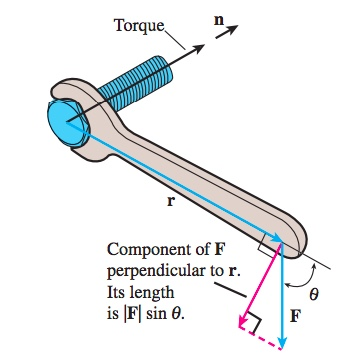
\includegraphics[scale=0.5]{figures_mvc/torque_wrench}
	\end{center}
\end{figure}

\begin{defn}[Cross product]
	The \emph{cross product} of two nonzero vectors $\mathbf{a}$ and $\mathbf{b}$ is the vector
	\begin{align*}
		\mathbf{a} \times \mathbf{b}=||\mathbf{a}|| \ ||\mathbf{b}||\sin\theta \mathbf{\hat{n}}
	\end{align*}
	where $\theta$ is the angle between $\mathbf{a}$ and $\mathbf{b}$ and $\mathbf{\hat{n}}$ is a unit vector in the direction determined by the \emph{right hand rule}, as illustrated in the figure below:
	\begin{figure}[h]
		\begin{center}
			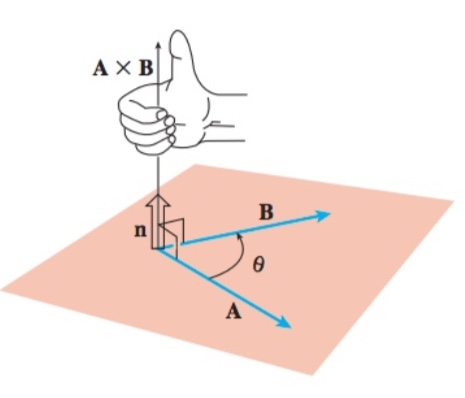
\includegraphics[scale=0.3]{figures_mvc/rhrule}
		\end{center}
	\end{figure}
	
	If either $\mathbf{a}$ or $\mathbf{b}$ is the zero vector, then we define $\mathbf{a} \times \mathbf{b}$ to be $\mathbf{0}$.
\end{defn}

\begin{example}
A 3 ft metal bar is hinged at one of its ends. If a 20 lb force is applied at the other endpoint at an angle of $70^\circ$ to the bar, then, choosing $xy$-coorindates centered at the hinge, the resulting torque is 
\begin{align*}
	||\vec{\tau}||=(3)(2)\sin(70^\circ)\mathbf{\hat{k}}.
\end{align*}
\begin{figure}[h]
	\begin{center}
		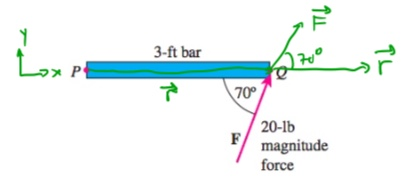
\includegraphics[scale=0.5]{figures_mvc/torque_example_bar}
	\end{center}
\end{figure}	
\end{example}

\subsubsection{Basic Properties of the Cross Product}

\begin{prop}[Geometry of the cross product]\label{prop:geometry_of_the_cross_product}
Let $\mathbf{a}$ and $\mathbf{b}$ be two nonzero vectors. Then
	\begin{enumerate}[(a)]
		\item $\mathbf{a} \times \mathbf{b}$ is orthogonal to both $\mathbf{a}$ and $\mathbf{b}$.
		\item $\mathbf{a}$ and $\mathbf{b}$ are parallel if and only if $\mathbf{a} \times \mathbf{b}=\mathbf{0}$.
		\end{enumerate}
\end{prop}

\begin{proof}
\begin{enumerate}[(a)]
	\item By the right hand rule, $\mathbf{a} \times \mathbf{b}$ is perpendicular to the plane containing $\mathbf{a}$ and $\mathbf{b}$. In particular, it is perpendicular to both $\mathbf{a}$ and $\mathbf{b}$.
	\item Since $\mathbf{a}$ and $\mathbf{b}$ are nonzero, $||\mathbf{a}||\neq 0$ and $||\mathbf{b}|| \neq 0$, and therefore $||\mathbf{a} \times \mathbf{b}||=||\mathbf{a}|| \ ||\mathbf{b}||\sin\theta=0$ if and only if $\sin \theta=0$. Since $0 \leq \theta \leq \pi$, $\sin \theta=0$ if and only if $\theta=0$ or $\pi$, that is, when the vectors $\mathbf{a}$ and $\mathbf{b}$ are parallel.
\end{enumerate}	
\end{proof}

\begin{remark}[The cross product is neither commutative nor associative] \hspace{15cm}
\begin{enumerate}[(a)]
	\item If $\mathbf{a} \times \mathbf{b}=||\mathbf{a}||\ ||\mathbf{b}||\sin\theta \mathbf{\hat{n}}$, then $\mathbf{b} \times \mathbf{a}=||\mathbf{a}||\ ||\mathbf{b}||\sin\theta \mathbf{(-\hat{n})}=-\mathbf{a} \times \mathbf{b}$, so the cross product is not commutative.
	\item Consider $\mathbf{a} \times (\mathbf{b} \times \mathbf{c})$. By part (a) of Proposition \ref{prop:geometry_of_the_cross_product}, $\mathbf{a} \times (\mathbf{b} \times \mathbf{c})$ is orthogonal to both $\mathbf{a}$ and $\mathbf{b} \times \mathbf{c}$. Since $\mathbf{b} \times \mathbf{c}$ is, in turn, orthogonal to both $\mathbf{b}$ and $\mathbf{c}$, $\mathbf{a} \times (\mathbf{b} \times \mathbf{c})$ is therefore perpendicular to a perpendicular to the plane containing $\mathbf{b}$ and $\mathbf{c}$, and his hence parallel to this plane. \fixme{Insert figure.} Repeating the same argument for $(\mathbf{a} \times \mathbf{b}) \times \mathbf{c}$, we find it is parallel to the plane containing $\mathbf{a}$ and $\mathbf{b}$. In general, $\mathbf{a}, \mathbf{b},$ and $\mathbf{c}$ will not lie in the same plane, so the cross products $\mathbf{a} \times (\mathbf{b} \times \mathbf{c})$ and  $(\mathbf{a} \times \mathbf{b}) \times \mathbf{c}$ will not lie in the same plane, and hence cannot be equal. This shows that the cross product is not associative.
\end{enumerate}
\end{remark}
We will now see that vector and scalar distributive laws \emph{do} hold for the cross product.
\begin{prop}[Scalar distributive law]\label{prop:scalar_distributive_law}
	Scalar multiplication distributes over the cross product. That is if $\mathbf{a},\mathbf{b}$ are vectors and $r,s$ scalars, then
	\begin{align*}
		(r\mathbf{a}) \times (s\mathbf{b})=(rs)(\mathbf{a} \times \mathbf{b}).
	\end{align*} 
\end{prop}

\begin{proof}
Let $\theta$ be the angle between $\mathbf{a}$ and $\mathbf{b}$, and let $\varphi$ be the angle between $r\mathbf{a}$ and $s\mathbf{b}$. Also, let $\mathbf{\hat{n}}$ be the unit vector determined by the right hand rule from $\mathbf{a}$ and $\mathbf{b}$, and $\mathbf{\hat{m}}$ be the unit vector determined by the right hand rule from $r\mathbf{a}$ and $s\mathbf{b}$. Then
\begin{align*}
	(r\mathbf{a}) \times (s\mathbf{b})&=||s\mathbf{b}|| \ ||s\mathbf{b}||\sin \varphi \ \mathbf{\hat{m}} \\
	&=|r|\ |s|\ ||\mathbf{a}|| \ ||\mathbf{b}|| \sin \varphi \ \mathbf{\hat{m}} \\
	&=|rs|\ ||\mathbf{a}|| \ ||\mathbf{b}|| \sin \varphi \ \mathbf{\hat{m}}
\end{align*}
We now have several cases to check, depending on $r$ and $s$.
\begin{enumerate}[(1)]
	\item If either $r=0$ or $s=0$, then both sides are $\mathbf{0}$, so equality holds.
	\item If $r>0$ and $s>0$, then $\varphi=\theta$, $\mathbf{\hat{m}}=\mathbf{\hat{n}}$, and $|rs|=rs$, so equality holds.
	\begin{figure}[h]
		\begin{center}
			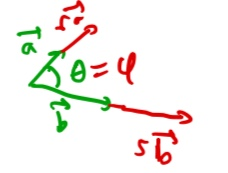
\includegraphics[scale=0.5]{figures_mvc/cp_proof_case_2}
		\end{center}
		\caption{Case (2).}
	\end{figure}
	\item If either $r<0$ and $s>0$ or $r>0$ and $s<0$, then $\varphi=\pi-\theta$, $\mathbf{\hat{m}}=-\mathbf{\hat{n}}$, and $|rs|=-rs$, and therefore
	\begin{align*}
		(r\mathbf{a}) \times (s\mathbf{b})&=-rs||\mathbf{a}|| \ ||\mathbf{b}||  \sin (\pi-\theta) \ (-\mathbf{\hat{n}}) \\
		&=rs||\mathbf{a}|| \ ||\mathbf{b}|| \sin\theta \mathbf{\hat{n}} \\
		&=rs (\mathbf{a} \times \mathbf{b})
	\end{align*}
	where we have used the fact that $\sin(\pi-\theta)=\sin\theta$.
	\begin{figure}[h]
		\begin{center}
			\includegraphics[scale=0.5]{figures_mvc/cp_proof_case_3}
		\end{center}
		\caption{Case (3).}
	\end{figure}
	\item If $r<0$ and $s<0$, then $\varphi=\theta$, $\mathbf{\hat{m}}=\mathbf{\hat{n}}$, and $|rs|=rs$, and therefore
	\begin{align*}
		(r\mathbf{a}) \times (s\mathbf{b})&=rs||\mathbf{a}|| \ ||\mathbf{b}||  \sin \theta \ \mathbf{\hat{n}} \\
		&=rs(\mathbf{a} \times \mathbf{b})
	\end{align*}
	\begin{figure}[h]
		\begin{center}
			\includegraphics[scale=0.3]{figures_mvc/cp_proof_case_4}
		\end{center}
		\caption{Case (4).}
	\end{figure}
\end{enumerate}
This exhausts the possibilities for $r$ and $s$, completing the proof.
\end{proof}

\begin{prop}[Vector distributive law]\label{prop:vector_distributive_law}
	The cross product distributes over vector addition. That is,
	\begin{align*}
		\mathbf{a} \times (\mathbf{b}+\mathbf{c})=\mathbf{a} \times \mathbf{b}+\mathbf{a} \times \mathbf{c}.
	\end{align*}
\end{prop}

\begin{proof}
	Let $\mathbf{a}, \mathbf{b},$ and $\mathbf{c}$ be vectors in three-dimensional space. If any of these are $\mathbf{0}$, then equality holds, so assume now that none of these are $\mathbf{0}$. We will prove the vector distributive law by constructing $\mathbf{a} \times \mathbf{b}$ in a clever way, as illustrated in the diagram below:
	\begin{figure}[h]
		\begin{center}
			\includegraphics[scale=0.5]{figures_mvc/cp_vector_dist_prop}
		\end{center}
		\caption{Steps to show that $\mathbf{a} \times \mathbf{b}=||\mathbf{a}||\mathbf{b}''$.}
	\end{figure}
	\begin{enumerate}[(1)]
		\item Let $M$ be the plane perpendicular to the plane containing $\mathbf{a}$ and $\mathbf{b}$, and let $\mathbf{b}'$ be the projection of $\mathbf{b}$ onto $M$. Letting $\theta$ denote the angle between $\mathbf{a}$ and $\mathbf{b}$, as usual, we have $||\mathbf{b}'||=||\mathbf{b}||\sin\theta$.
		\item Now rotate $\mathbf{b}'$ by $90^\circ$ counterclockwise about $\mathbf{a}$ to obtain $\mathbf{b}''$. Scalar multiplying $\mathbf{b}''$ by $||\mathbf{a}||$, we obtain the vector $||\mathbf{a}||\mathbf{b}''$. Noting that
		\begin{align*}
			||\ (||\mathbf{a}|| \mathbf{b}'') \ ||=||\mathbf{a}|| \ ||\mathbf{b}''|| = ||\mathbf{a}|| \ ||\mathbf{b}'||=||\mathbf{a}|| \ ||\mathbf{b}||\sin \theta
		\end{align*}
		and that $||\mathbf{a}||\mathbf{b}''$ is orthogonal to both $\mathbf{a}$ and $\mathbf{b}$ and points in the direction given by the right hand rule, we see that 
		\begin{align}\label{eq:clever_b}
			||\mathbf{a}||\mathbf{b}''=\mathbf{a} \times \mathbf{b}
		\end{align}
		as these two vectors have the same magnitude and direction.
		\item Repeating the exact same steps with $\mathbf{c}$, we obtain
		\begin{align}\label{eq:clever_c}
			||\mathbf{a}||\mathbf{c}''=\mathbf{a} \times \mathbf{c}.
		\end{align}
		\item Consider now a triangle with legs $\mathbf{b}, \mathbf{c},$ and $\mathbf{b}+\mathbf{c}$. 
	\begin{figure}[h]
		\begin{center}
			\includegraphics[scale=0.5]{figures_mvc/cp_proof_triangle_1}
		\end{center}
		\caption{Triangle from step (4), when $\mathbf{a}, \mathbf{b},$ and $\mathbf{c}$ do not all lie in the same plane. \fixme{Crop out writing in the corner of graphic.}}
	\end{figure}
	
		If the plane of the triangle does not contain $\mathbf{a}$, then after projecting this triangle onto $M$, rotating by $90^\circ$ counterclockwise about $\mathbf{a}$, and multiplying each leg by $||\mathbf{a}||$, we obtain a triangle in the plane $M$ with legs $\mathbf{b}'', \mathbf{c}'',$ and $(\mathbf{b}+\mathbf{c})''$, which satisfy
		\begin{align}\label{eq:triangle_cp}
			||\mathbf{a}||\mathbf{b}''+||\mathbf{a}||\mathbf{c}''=||\mathbf{a}||(\mathbf{b}+\mathbf{c})''.
		\end{align}
		Substituting \eqref{eq:clever_b} and \eqref{eq:clever_c} into \eqref{eq:triangle_cp} then gives
		\begin{align*}
			\mathbf{a} \times \mathbf{b}+\mathbf{a} \times \mathbf{c}=\mathbf{a} \times (\mathbf{b}+\mathbf{c}),
		\end{align*}
		as desired.
		\item Finally, if the vectors $\mathbf{a}, \mathbf{b}$, and $\mathbf{c}$ all lie in the same plane, then the triangle with legs $\mathbf{b}, \mathbf{c},$ and $\mathbf{b}+\mathbf{c}$ when projected onto $M$ projects to a line segment. 
		\begin{figure}[h]
		\begin{center}
			\includegraphics[scale=0.3]{figures_mvc/cp_proof_triangle_2}
		\end{center}
		\caption{Triangle from step (5), when $\mathbf{a}, \mathbf{b},$ and $\mathbf{c}$ all lie in the same plane.}
	\end{figure}
	
		It then follows from the segment addition postulate that $(\mathbf{b}+\mathbf{c})'=\mathbf{b}'+\mathbf{c}'$. The rest of the proof then follows the same steps above, so we have now shown that equality holds for all vectors $\mathbf{a}, \mathbf{b},$ and $\mathbf{c}$.
	\end{enumerate}
\end{proof}

\subsubsection{Cross Product in Coordinates}
As we have seen in Section \ref{sec:vectors_and_geometry}, the study of the properties of vectors in three-dimensional space is greatly facilitated by choosing a Cartesian coordinate system. To write the cross product of two vectors 
\begin{align*}
	\mathbf{a}&=a_1\mathbf{\hat{i}}+a_2\mathbf{\hat{j}}+a_3\mathbf{\hat{k}}, \\
	\mathbf{b}&=b_1\mathbf{\hat{i}}+b_2\mathbf{\hat{j}}+b_3\mathbf{\hat{k}}, \\
\end{align*}
in terms of their components, we begin by working out the cross products of the standard unit vectors $\mathbf{\hat{i}}, \mathbf{\hat{j}},$ and $\mathbf{\hat{k}}$. We note immediately that $\mathbf{\hat{i}} \times \mathbf{\hat{i}}=\mathbf{\hat{j}} \times \mathbf{\hat{j}}=\mathbf{\hat{k}} \times \mathbf{\hat{k}}=\mathbf{0}$ by part (b) of Proposition \ref{prop:geometry_of_the_cross_product}. Since the distinct vectors are all mutually orthogonal, by the right hand rule we find
\begin{align*}
	\mathbf{\hat{i}} \times \mathbf{\hat{j}}&=\mathbf{\hat{k}}, \\
	\mathbf{\hat{j}} \times \mathbf{\hat{k}}&=\mathbf{\hat{i}}, \\
	\mathbf{\hat{k}} \times \mathbf{\hat{i}}&=\mathbf{\hat{j}}
\end{align*}
while 
\begin{align*}
	\mathbf{\hat{j}} \times \mathbf{\hat{i}}&=-\mathbf{\hat{k}}, \\
	\mathbf{\hat{k}} \times \mathbf{\hat{j}}&=-\mathbf{\hat{i}}, \\
	\mathbf{\hat{i}} \times \mathbf{\hat{k}}&=-\mathbf{\hat{j}}.
\end{align*} 
\fixme{Insert wheel graphic.}

We can now use the scalar and vector distributive laws from Propositions \ref{prop:scalar_distributive_law} and \ref{prop:vector_distributive_law}, as well as the cross products of the standard unit vectors, to work out a formula for the components of $\mathbf{a} \times \mathbf{b}$. Let 
	\begin{align*}
	\mathbf{a}&=a_1\mathbf{\hat{i}}+a_2\mathbf{\hat{j}}+a_3\mathbf{\hat{k}}, \\
	\mathbf{b}&=b_1\mathbf{\hat{i}}+b_2\mathbf{\hat{j}}+b_3\mathbf{\hat{k}}, \\
\end{align*}
be any two vectors. Then
\begin{align*}
	\mathbf{a} \times \mathbf{b}&=(a_1\mathbf{\hat{i}}+a_2\mathbf{\hat{j}}+a_3\mathbf{\hat{k}}) \times (b_1\mathbf{\hat{i}}+b_2\mathbf{\hat{j}}+b_3\mathbf{\hat{k}}) \\
	&=a_1b_1\underbrace{(\mathbf{\hat{i}} \times \mathbf{\hat{i}})}_{=\mathbf{0}}+a_1b_2\underbrace{(\mathbf{\hat{i}} \times \mathbf{\hat{j}})}_{=\mathbf{\hat{k}}}+a_1b_3\underbrace{(\mathbf{\hat{i}} \times \mathbf{\hat{k}})}_{=-\mathbf{\hat{j}}} \\
	&+a_2b_1\underbrace{(\mathbf{\hat{j}} \times \mathbf{\hat{i}})}_{=-\mathbf{\hat{k}}}+a_2b_2\underbrace{(\mathbf{\hat{j}} \times \mathbf{\hat{j}})}_{=\mathbf{0}}+a_2b_3\underbrace{(\mathbf{\hat{j}} \times \mathbf{\hat{k}})}_{=\mathbf{\hat{i}}} \\
	&+a_3b_1\underbrace{(\mathbf{\hat{k}} \times \mathbf{\hat{i}})}_{=\mathbf{\hat{j}}}+a_3b_2\underbrace{(\mathbf{\hat{k}} \times \mathbf{\hat{j}})}_{=-\mathbf{\hat{i}}}+a_3b_3\underbrace{(\mathbf{\hat{k}} \times \mathbf{\hat{k}})}_{=\mathbf{0}}
	\end{align*}
	and collecting like terms gives
	\begin{align}\label{eq:cp_comp}
		\mathbf{a} \times \mathbf{b}&=(a_2b_3-a_3b_2)\mathbf{\hat{i}}-(a_1b_3-a_3b_1)\mathbf{\hat{j}}+(a_1b_2-a_2b_1)\mathbf{\hat{k}}.
	\end{align}
Note that the formula in Equation \eqref{eq:cp_comp} is exactly what one would obtain by \emph{formally} taking the determinant of the `matrix'
\begin{align*}
	\begin{vmatrix}
		\mathbf{\hat{i}} & \mathbf{\hat{j}} & \mathbf{\hat{k}} \\
		a_1 & a_2 & a_3 \\
		b_1 & b_2 & b_3 
	\end{vmatrix},
\end{align*}
where the `matrix' above has the standard unit vectors as entries in the first row, rather than numbers. \footnote{The use of the word `formally' here reflects the fact that the determinant is a function which is really only defined for matrices whose entries are numbers, and not a matrix whose entries are a mix of numbers and vectors, as we have not actually defined such a beast.}

\begin{prop}[Determinant formula for the cross product]\label{prop:determinant_formula_for_the_cross_product}
	The cross product of two vectors 
	\begin{align*}
	\mathbf{a}&=a_1\mathbf{\hat{i}}+a_2\mathbf{\hat{j}}+a_3\mathbf{\hat{k}}, \\
	\mathbf{b}&=b_1\mathbf{\hat{i}}+b_2\mathbf{\hat{j}}+b_3\mathbf{\hat{k}}, \\
\end{align*}
has components given by the following formal determinant: 
\begin{align*}
	\mathbf{a} \times \mathbf{b}&=\begin{vmatrix}
		\mathbf{\hat{i}} & \mathbf{\hat{j}} & \mathbf{\hat{k}} \\
		a_1 & a_2 & a_3 \\
		b_1 & b_2 & b_3 
	\end{vmatrix} \\
	&=(a_2b_3-a_3b_2)\mathbf{\hat{i}}-(a_1b_3-a_3b_1)\mathbf{\hat{j}}+(a_1b_2-a_2b_1)\mathbf{\hat{k}}.
\end{align*}
\end{prop}

\begin{exercise}
\begin{enumerate}[(a)]
	\item Use the determinant formula in Proposition \ref{prop:determinant_formula_for_the_cross_product} to find the cross product $\mathbf{a} \times \mathbf{b}$ when $\mathbf{a}=(1,2,-2)$ and $\mathbf{b}=(3,0,1)$.
	\item Compute $\mathbf{a} \times \mathbf{b}$ and $\mathbf{b} \times \mathbf{a}$ if $\mathbf{a}=(2,1,1)$ and $\mathbf{b}=(-4,3,1)$.
\end{enumerate}	
\end{exercise}

\begin{thm}[Properties of the cross product]\label{thm:props_cp}
	If $\mathbf{a},\mathbf{b},$ and $\mathbf{c}$ are any vectors in three-dimensional space and $k$ is any scalar, then:
	\begin{enumerate}[(a)]
		\item $\mathbf{a} \times \mathbf{b}=-\mathbf{b} \times \mathbf{a}$,
		\item $\mathbf{a} \times (\mathbf{b}+\mathbf{c})=\mathbf{a} \times \mathbf{b}+\mathbf{a} \times \mathbf{c})$,
		\item $(k\mathbf{a}) \times \mathbf{b}=\mathbf{a} \times (k\mathbf{b})=k(\mathbf{a} \times \mathbf{b})$
		\item $\mathbf{a} \times \mathbf{a}$
	\end{enumerate}
\end{thm}

\begin{exercise}
We have proved Theorem \ref{thm:props_cp} already. Reprove it using the determinant formula in Proposition \ref{prop:determinant_formula_for_the_cross_product}.
\end{exercise}

\subsubsection{Applications to Geometry}
Note that, geometrically, the magnitude of the cross product of two nonzero vectors $\mathbf{a}$ and $\mathbf{b}$
\begin{align*}
	||\mathbf{a} \times \mathbf{b}||=||\mathbf{a}|| \ ||\mathbf{b}||\sin\theta
\end{align*}
is the area of the parallelogram whose adjacent sides are formed by $\mathbf{a}$ and $\mathbf{b}$:
\begin{figure}[h]
	\begin{center}
		\includegraphics[scale=0.5]{figures_mvc/cp_pg}
	\end{center}
\end{figure}

\begin{example}
To find the area of the triangle with vertices $A(2,0), B(3,4)$, and $C(-1,2)$, we first form the vectors $\overrightarrow{AB}=(3-2,4-0)=(1,4)$ and $\mathbf{AC}=(-1-2,2-0)=(-3,2)$. Since the area of the triangle whose legs are $\overrightarrow{AB}, \overrightarrow{AC},$ and $\overrightarrow{AB}-\overrightarrow{AC}$ is half the area of the parallelogram whose adjacent sides are formed by $\overrightarrow{AB}$ and $\overrightarrow{AC}$, we compute the area by taking half the magnitude of the cross product of these two vectors:
\begin{align*}
	\text{Area}&=\frac{1}{2}||\overrightarrow{AB}\times \overrightarrow{AC}|| \\
	&=\frac{1}{2} || \begin{vmatrix}
		\mathbf{\hat{i}} & \mathbf{\hat{j}} & \mathbf{\hat{k}} \\
		1 & 4 & 0 \\
		-3 & 2 & 0
	\end{vmatrix} || \\
	&=\frac{1}{2}||(2+12)\mathbf{\hat{k}}|| \\
	&=\frac{1}{2}|14| \ ||\mathbf{\hat{k}}|| \\
	&=7 \text{ (units)}^2.
\end{align*}	
\end{example}

\begin{exercise}
Find the area of the triangle with vertices $A(1,1), B(2,2), C(3,-3)$. \emph{Hint: To compute the cross product, write each of these vectors as a vector in $\mathbb{R}^3$, whose $z$-component is 0.}	
\end{exercise}

\begin{exercise}
Find a vector perpendicular to the plane defined by the points $P(1,-1,0), Q(2,1,-1),$ and $R(-1,1,2)$. Find a unit normal to this plane.	
\end{exercise}

\begin{exercise}
Find a vector parallel to the line of intersection of the planes
\begin{align*}
	3x-6y-2z&=15, \\
	2x+y-2z&=5.
\end{align*}	
\end{exercise}

\subsection{Triple Scalar Product}
Since $\mathbf{a} \times \mathbf{b}$ is a vector, the product $\mathbf{a} \times \mathbf{b} \cdot \mathbf{c}$ is defined. This product actually comes up frequently, so we will discuss its properties in this section.
\begin{defn}[Triple scalar product]
	For any vectors $\mathbf{a}, \mathbf{b}$, and $\mathbf{c}$ the \emph{triple scalar product} is defined by 
	\begin{align*}
		\mathbf{a} \times \mathbf{b} \cdot \mathbf{c}=||\mathbf{a} \times \mathbf{b}|| \ ||\mathbf{c}||\cos \theta,
	\end{align*}
	where $\theta$ is the angle between $\mathbf{a} \times \mathbf{b}$ and $\mathbf{c}$.
\end{defn}

\begin{prop}[Determinant formula for the triple scalar product]\label{prop:det_formula_for_stp}
	The triple scalar product is given by
	\begin{align*}
		(\mathbf{a} \times \mathbf{b}) \cdot \mathbf{c}&=\begin{vmatrix}
			c_1 & c_2 & c_3 \\
			a_1 & a_2 & a_3 \\
			b_1 & b_2 & b_3
		\end{vmatrix} \\
		&=(a_2b_3-a_3b_2)c_1-(a_1b_3-a_3b_1)c_2+(a_1b_2-a_2b_1)c_3.
	\end{align*}
\end{prop}

\begin{exercise}
Use the determinant formula for the cross product from Proposition \ref{prop:determinant_formula_for_the_cross_product} to prove this.
\end{exercise}

\begin{prop}[Cyclic symmetry of the triple scalar product]
	The triple scalar product is invariant under cyclic permutation of the vectors $\mathbf{a}, \mathbf{b},$ and $\mathbf{c}$:
	\begin{align*}
		(\mathbf{a} \times \mathbf{b})\cdot \mathbf{c}=(\mathbf{b} \times \mathbf{c})\cdot \mathbf{a}=(\mathbf{c} \times \mathbf{a})\cdot \mathbf{b}.
	\end{align*}
\end{prop}

\begin{exercise}
Prove this using the fact that a row interchange changes the sign of the determinant.	
\end{exercise}

\begin{prop}[Interchange of dot and cross product in triple scalar product]
	The triple scalar product is invariant under exchanging the dot and cross product, in the sense that 
	\begin{align*}
		(\mathbf{a} \times \mathbf{b})\cdot \mathbf{c}=\mathbf{a} \cdot (\mathbf{b}\times \mathbf{c}).
	\end{align*}
\end{prop}

\begin{exercise}
Prove this using the cyclic symmetry of the cross product together with the symmetry of the dot product.	
\end{exercise}

\begin{prop}[Relationships between dot and cross product]
We have the following relationships between the dot and cross products:
	\begin{figure}[h]
			\includegraphics[scale=0.3]{figures_mvc/rel_dot_cross_p}
	\end{figure}
\end{prop}

\begin{exercise}
Prove these.	
\end{exercise}

Geometrically, the magnitude of $(\mathbf{a} \times \mathbf{b})\cdot \mathbf{c}$ is the volume of the parallelepiped whose adjacent sides are $\mathbf{a},\mathbf{b}$, and $\mathbf{c}$. The number $||\mathbf{a} \times \mathbf{b}||$ is the area of the base parallelogram, while $||\mathbf{c}||\cos \theta$ is the height of the paralleleliped.
\begin{figure}[h]
	\begin{center}
		\includegraphics[scale=0.5]{figures_mvc/ppiped}
	\end{center}
\end{figure}
For this reason, the triple scalar product is also sometimes referred to as the \emph{box product} of $\mathbf{a},\mathbf{b}$, and $\mathbf{c}$.

\begin{exercise}
Use the triple scalar product to show that the volume of the parallelepiped with adjacent sides $\mathbf{a}=(1,2,-1), \mathbf{b}=(-2,0,3)$, and $\mathbf{c}=(0,7,-4)$ is 23 (units)$^3$.	
\end{exercise}

\begin{prop}[Geometric interpretation of determinants]
We have the following geometric interpretation of determinants:
	\begin{figure}[h]
			\begin{center}
				\includegraphics[scale=0.4]{figures_mvc/whole_enchilada}
			\end{center}
	\end{figure}
\end{prop}

\section{Vector Spaces}\label{sec:vector_spaces}
We have seen previously that various diverse applications, such as analyzing electrical circuits and balancing chemical equations, could all be solved in exactly the same way: since the solution of the problem involved forming linear combinations of a fixed number of unknown quantities, this gave rise to a system of linear equations which we were able to solve by our row-reduction algorithm. We therefore find it useful to generalize our concept of a vector, abstracting the essential properties which make it possible to solve any system which shares these properties. This gives rise to the notion of a \emph{vector space}.

\subsection{Basic Definitions and Examples}\label{sec:basic_definitions_and_examples}
\begin{defn}[Vector space] \label{def:vector_space}
	Let $V$ be a set and $\mathbb{R}$ be the set of real numbers. Define a function
\begin{align*}
	+:V\times V &\to V \\
	({\bf v},{\bf w}) &\mapsto {\bf v}+{\bf w}
\end{align*}
called \emph{vector addition} (or just \emph{addition}) and a function
\begin{align*}
	\cdot :\mathbb{R}\times V &\to V \\
	(x,{\bf v}) &\mapsto x{\bf v}
\end{align*}
called \emph{scalar multiplication}. \footnote{Rather than write $x \cdot \mathbf{v}$, it is more common to just write $x\mathbf{v}$.} The ordered triple $(V,+,\cdot)$ is called a \emph{real vector space} (or just a \emph{vector space}) if the following axioms hold: \\
\\
{\bf A1.} (Associativity of addition) ${\bf u}+({\bf v}+{\bf w})=({\bf u}+{\bf v})+{\bf w}$ for all  ${\bf u},{\bf v}, {\bf w} \in V$. \\
{\bf A2.} (Commutativity of addition) ${\bf u}+{\bf v}={\bf v}+{\bf u}$ for all ${\bf u}, {\bf v} \in V$. \\
{\bf A3.} (Existence of an additive identity) There exists an element ${\bf 0} \in V$ such that ${\bf v}+{\bf 0}={\bf v}$ for all ${\bf v} \in V$. \\
{\bf A4.} (Existence of additive inverses) For every ${\bf v} \in V$ there exists a ${\bf w} \in V$ such that ${\bf v}+{\bf w}={\bf 0}$. \\
\\
{\bf S1.} (Associativity of multiplication) $(xy){\bf v}=x(y{\bf v})$ for all $x,y \in \mathbb{R}, {\bf v}\in V$. \\
{\bf S2.} (Distributivity over scalar addition) $(x+y){\bf v}=x{\bf v}+y{\bf v}$ for all $x,y \in \mathbb{R}, {\bf v} \in V$ \\
{\bf S3.} (Distributivity over vector addition) $x({\bf v}+{\bf w})=x{\bf v}+x{\bf w}$ for all $x \in \mathbb{R}, {\bf v}, {\bf w} \in V$. \\
{\bf S4.} (Multiplication by 1 fixes each vector) $1{\bf v}={\bf v}$ for all ${\bf v} \in V$. 
\end{defn}
If the operations $+,\cdot$ are clear from context, then it is common to simply refer to $V$ as a vector space.

Elements of a vector space $V$ are called \emph{vectors} and elements of $\mathbb{R}$ are called \emph{scalars}. \footnote{Since the scalars here are just real numbers, why call them scalars and not just continue to refer to them as real numbers? One reason is that this terminology is historical, coming from physics. Another is the following: If we replace $\mathbb{R}$ with $\mathbb{C}$ in the definition of a vector space, we get the definition of a \emph{complex vector space}. More generally, we can replace $\mathbb{R}$ in the definition of a vector space with any  \emph{field} $\mathbb{F}$, which is a set with two binary operations (called \emph{addition} and \emph{multiplication}), which have the same properties as ordinary addition and multiplication of real numbers ($\mathbb{C}$ is an example). This gives us a \emph{vector space over} $\mathbb{F}$. Most of the theory which will be developed going forward actually holds for a vector space over any field, so it is more common to just refer to elements of $\mathbb{R}$ as scalars to keep one's options open. However, in this class we will always take our scalars to be real numbers. This is actually slightly a lie, since in the next unit we will sometimes take them to be polynomials (which do not form a field since non-constant polynomials do not have multiplicative inverses), but these subtleties will not cause us any trouble at this level of study.}

Let us now consider various examples of vector spaces. We begin with the simplest possible example of a vector space:

\begin{example}[The zero vector space]\label{ex:zero_vector_space}
	Let $V=\{0\}$ and define $0+0:=0$ and $x0:=0$ for all $x \in \mathbb{R}$. It is easy to check that A1-S4 are satisfied, so this is a vector space. This is called the \emph{zero vector space} or the \emph{trivial vector space}.
\end{example}

\begin{exercise}
Check that the zero vector space is indeed a vector space.
\end{exercise}


Of course, $\mathbb{R}^n$ is another example of a vector space, since we \emph{defined} a vector space to have the algebraic properties of $\mathbb{R}^n$. 

\begin{example}[$\mathbb{R}^n$]\label{ex:r_n}
	Let $V=\mathbb{R}^n$ and define
\begin{align*}
	{\bf v}+{\bf w} &:=(v_1+w_1,v_2+w_2,\cdots, v_n+w_n) \\
	x{\bf v} &:=(xv_1, xv_2, \cdots, xv_n).
\end{align*} These satisfy the vector space axioms because \emph{we based these axioms} on known properties of $\mathbb{R}^n$.
\end{example}

We can also consider \emph{infinite} sequences of elements of $\mathbb{F}$:

\begin{example}[$\mathbb{R}^\omega$]\label{ex:r_omega}
	Let $\mathbb{R}^\omega$ denote the set of infinite sequences of elements of $\mathbb{R}$. An element of $\mathbb{R}^\omega$ is therefore of the form 
	\begin{align*}{\bf v}=(v_1,v_2,\cdots, v_n,\cdots)
	\end{align*} 
	where we take ${\bf v}={\bf w}$ if and only if $v_i=w_i$ for all $i$. Defining addition and scalar multiplication componentwise by
	\begin{align*}
		{\bf v}+{\bf w} &:=(v_1+w_1,v_2+w_2,\cdots, v_n+w_n,\cdots) \\
	x{\bf v} &:=(xv_1, xv_2, \cdots, xv_n,\cdots)
	\end{align*}
	one can verify that $\mathbb{R}^\omega$ is a vector space. \footnote{For the reader wondering about the notation, the symbol $\omega$ denotes the first infinite \emph{ordinal}, which is most likely an unfamiliar concept. For those who are interested, I encourage you to go ask Michael Rawlins about ordinal numbers.}
\end{example}

We have seen that matrices are composed of vectors (rows and columns). However, as we will now see, we can also view the \emph{entire} matrix itself as a vector.

\begin{example}[$M^{m \times n}(\mathbb{R})$]\label{ex:m_by_n}
	Let $M^{m \times n}(\mathbb{R})$ denote the set of $m \times n$ matrices with entries in $\mathbb{R}$. This is a vector space under the usual componentwise addition and scalar multiplication:
	\begin{align*}
		(a+b)_{ij}&=a_{ij}+b_{ij} \\
		(xa)_{ij}&=xa_{ij}
	\end{align*}
\end{example}

All of these examples so far were obtained by replacing $\mathbb{R}^n$ by another set $V$, but keeping essentially the same operations. In the next example, we illustrate the flexibility in choice of vector addition and scalar multiplication.

\begin{example}[An "unusual" vector space]\label{ex:unusual_vector_space}
	Let $V$ be the set positive real numbers, $\mathbb{R}^+$, and define vector addition to be ordinary multiplication and scalar multiplication to be exponentiation. That is, for any $u,v \in \mathbb{R}^+$ and $k \in \mathbb{R}$,
	\begin{align*}
		u+v&=uv \\
		ku&=u^k 
	\end{align*}
	With these definitions, we have, for instance, $1+1=(1)(1)=1$ and $(2)(1)=1^2=1$. If this is to be a vector space, we see that the zero vector must be ${\bf 0}=1$, since 
	\begin{align*}
		u+1=(u)(1)=u
	\end{align*}
	and that the additive inverse of $u$ is its reciprocal $\frac{1}{u}$, since
	\begin{align*}
		u+\frac{1}{u}=(u)(\frac{1}{u})=1={\bf 0}
	\end{align*}
One can check that all the vector space axioms are satisfied. For instance, axiom S4 holds due to the properties of exponents:
\begin{align*}
	k(u+v)=(uv)^k=u^kv^k=(ku)+(kv).
\end{align*}
\end{example}

\begin{exercise}
	Verify that Example \ref{ex:unusual_vector_space} is a vector space.
\end{exercise}

While the previous example shows that it is possible to give the same set different vector space structures, not every choice of operations will give rise to a vector space.

\begin{exercise}
Let $V=\mathbb{R}^2$ and define vector addition as usual, but scalar multiplication as 
\begin{align*}
	k(v_1,v_2)&=(kv_1,0).
\end{align*}	
Show that this is not a vector space. Which axiom(s) fail to hold?
\end{exercise}

\begin{example}
Let $V=\{(x,y) \in \mathbb{R}^2:x \geq 0\}$ and define vector addition and scalar multiplication as the usual ones for $\mathbb{R}^2$. 
\begin{align*}
	(x_1,y_1)+(x_2,y_2)&:=(x_1+x_2,y_1+y_2) \\
	k(x,y)&:=(kx,ky).
\end{align*}

Vector addition is a well-defined function $V \times V \to V$, since $x_1 \geq 0$ and $x_2 \geq 0$ together imply that $x_1+x_2 \geq 0$. However, if $k=-1$, then $(-x,-y)$ is not an element of $V$ if $x>0$. Thus, this is not a vector space since scalar multiplication is not a well-defined function $\mathbb{R} \times V \to V$.
\end{example}

\subsection{Vector Space Properties}
There are additional properties of any vector space which follow directly from Definition \ref{def:vector_space}.

\begin{thm}[Properties of vector spaces]\label{thm:properties_of_vector_spaces}
	Let $V$ be a vector space, ${\bf v} \in V$, and $x \in \mathbb{R}$. Then:
	\begin{enumerate}[(a)]
		\item The element ${\bf 0} \in V$ of A3 is unique.
		\item $x{\bf 0}={\bf 0}$ for all $x\in \mathbb{R}$ 
		\item $0{\bf v}={\bf 0}$ for all ${\bf v} \in V$.
		\item For each ${\bf v}$ the ${\bf w}$ of A4 is unique. We denote this vector by $-{\bf v}$.
		\item $-{\bf v}=(-1){\bf v}$ for all ${\bf v} \in  V$.
		\item If $x{\bf v}={\bf 0}$, then either $x=0$ or ${\bf v}={\bf 0}$.
	\end{enumerate}
\end{thm}

\begin{pf}
(a) Suppose ${\bf 0},{\bf 0'} \in V$ such that 
\begin{align}
	{\bf 0}+{\bf v} &={\bf v} \\
	{\bf 0'}+{\bf v} &={\bf v}
\end{align}
for all ${\bf v} \in V$. Then 
\begin{align*}
	{\bf 0'}&={\bf 0}+{\bf 0'} \text{ (by (1))} \\
	&={\bf 0} \text{ (by (2))} \\
\end{align*}
Hence, ${\bf 0}$ is unique. 

(b) We have, by A3, x{\bf 0}=x{\bf 0}+{\bf 0}. We also have
\begin{align*}
	x{\bf 0}&=x({\bf 0}+{\bf 0}) \text{ (since ${\bf 0}={\bf 0}+{\bf 0}$ by A3)} \\
	&=x{\bf 0}+x{\bf 0} \text{ (by S3)}
\end{align*} and therefore $x{\bf 0}+x{\bf 0}=x{\bf 0}+{\bf 0}$. Adding the inverse of $x{\bf 0}$ to both sides (A4), and using (A1), we find $x{\bf 0}={\bf 0}$.	
(c) Applying A3, we have $0{\bf v}=0{\bf v}+{\bf 0}$. We also have
$0{\bf v} =(0+0){\bf v}=0{\bf v} + 0{\bf v}$ by S2. Letting ${\bf w}$ be the inverse of $0{\bf v}$ (which exists by A4), we have
\begin{align*}
	0{\bf v}+{\bf 0}&=0{\bf v}+0{\bf v} \\
	{\bf w}+0{\bf v}+{\bf 0}&={\bf w}+0{\bf v}+0{\bf v} \\
	({\bf w}+0{\bf v})+{\bf 0}&=({\bf w}+0{\bf v})+0{\bf v} \text{ (by A1)}\\
	0+{\bf 0}&=0+0{\bf v} \text{ (by A4)}
\end{align*} and therefore $0{\bf v}={\bf 0}$. 

(d) Suppose for some ${\bf v} \in V$ there exist ${\bf w},{\bf w'} \in V$ such that
\begin{align}
	{\bf v}+{\bf w} &={\bf 0} \\
	{\bf v}+{\bf w'} &={\bf 0}
\end{align} Then
\begin{align*}
	{\bf w'}&={\bf w'}+{\bf 0} \text{ (by A3)}\\
	&={\bf w'}+({\bf v}+{\bf w}) \text{ (by (3))} \\
	&=({\bf w'}+{\bf v})+{\bf w} \text{ (by A1)} \\
	&={\bf 0}+{\bf w} \text{ (by (4))} \\
	&={\bf w} \text{ (by A3).}
\end{align*} Hence, for each ${\bf v}$, ${\bf w}\equiv -{\bf v}$ is unique.

(e) We have
	\begin{align*}
		{\bf v}+(-1){\bf v} &=1{\bf v}+(-1){\bf v} \text{ (by S4)}\\
		&=(1+(-1)){\bf v} \text{ (by S2)}\\
		&=0{\bf v} \\
		&={\bf 0} \text{ by (c)}
	\end{align*}
By (d), for each ${\bf v} \in V$ there exists a unique $-{\bf v}$ such that ${\bf v}+(-{\bf v})=0$. Hence, $-{\bf v}=(-1){\bf v}$.

(f) Suppose $x{\bf v}={\bf 0}$. Then $x{\bf v}=0{\bf v}$ by (c) and therefore $x{\bf v}+(-0{\bf v})=0{\bf v}+(-0{\bf v})=0$ by A4. Applying (e), we have $(x-0){\bf v}={\bf 0}$. If $x=0$, we are done. If $x \neq 0$, we can multiply both sides by $\frac{1}{x-0}=\frac{1}{x}$ and we have ${\bf v}={\bf 0}$.
\end{pf}

We have just seen that the vector space structure establishes a connection between such diverse mathematical objects such as geometric vectors, vectors in $\mathbb{R}^n$, infinite sequences, matrices, and real-valued functions, to name a few. Consequently, whenever we prove a new theorem which holds for a general vector space (such as Theorem \ref{thm:properties_of_vector_spaces}), it will apply to \emph{all} of these vector spaces.

\subsection{$\mathbb{R}^A$}\label{sec:r_a}
We can obtain a large number of examples of vector spaces in the following way. Note that, in Examples \ref{ex:r_n}, \ref{ex:r_omega}, and \ref{ex:m_by_n} above, the reason why the vector space axioms were satisfied was essentially because they are satisfied for real numbers. We can exploit this to systematically find other examples of vector spaces.

Let $\overline{n}$ denote the first $n$ positive integers; that is, $\overline{n}:=\{1,2,\dots,n\}$. We can view an ordered $n$-tuples $\mathbf{x}=(x_1,x_2,\dots,x_n) \in \mathbb{R}^n$ as a \emph{function} 
\begin{align*}
	\mathbf{x}:\overline{n} \to \mathbb{R}
\end{align*}
defined by $\mathbf{x}(i)=x_i$. From this point of view, vector addition and scalar multiplication are just the usual definitions of pointwise addition and scalar multiplication of functions:
\begin{align*}
	({\bf x}+{\bf y})(i)&={\bf x}(i)+{\bf y}(i) \\
	&=x_i+y_i \\
	(c{\bf x})(i)&=c{\bf x}(i) \\
	&=cx_i.
\end{align*}
Now, replace $\overline{n}\equiv \{1,2,\cdots,n\}$ by \emph{any} set $A$.
	Denote by $\mathbb{R}^A$ the set of all functions from $A$ into $\mathbb{R}$, that is, $\mathbb{R}^A\equiv \{f|f:A \to \mathbb{R}\}$. This set is again a vector space under the operations
 \begin{align}\label{eq:pointwise_1}
	(f+g)(a)&=f(a)+g(a) \text{ for all } a \in A\\ \label{eq:pointwise_2}
	(xf)(a)&=xf(a) \text{ for all } a \in A, x \in \mathbb{R} 
\end{align}
It then follows immediately that $\mathbb{R}^A$ is a vector space because $\mathbb{R}$ is (we will prove this in Proposition \ref{prop:r_a_is_a_vector_space} below).

\begin{example}
Let $f(x), g(x) \in \mathbb{R}^\mathbb{R}$ (the vector space of all functions $\mathbb{R} \to \mathbb{R}$), where $f(x)=\sin(x)$ and $g(x)=e^x$. Then their vector sum is given by
\begin{align*}
	(f+g)(x)&=f(x)+g(x)=\sin(x)+e^x \\
\end{align*}
and the scalar multiple of $f(x)$ by $\sqrt{\pi}$ is given by
\begin{align*}
	(\sqrt{\pi}f)(x)&=\sqrt{\pi}f(x)=\sqrt{\pi}\sin(x).
\end{align*}	
\end{example}

\begin{figure}[h]
	\begin{center}
	\includegraphics[scale=0.5]{figures_mvc/function_operations}
\end{center}
\caption{Visualization of the operations \eqref{eq:pointwise_1} and \eqref{eq:pointwise_2} for continuous functions from $\mathbb{R} \to \mathbb{R}$. The figure in (a) illustrates a vector sum, (b) illustrates a scalar multiple, and (c) an additive inverse.}
\end{figure}


\begin{prop}[$\mathbb{R}^A$ is a vector space]\label{prop:r_a_is_a_vector_space}
The set $\mathbb{R}^A$ is a vector space under the operations \eqref{eq:pointwise_1} and \eqref{eq:pointwise_2}.
\end{prop}

\begin{proof}
We will show that A1-A4, S1-S4 of Definition \ref{def:vector_space} hold. The key fact is that the values $f(a)$ of a function $f \in \mathbb{R}^A$ are real numbers. The reader should be able to justify each step in what follows.  \\
\\
{\bf A1.} Let $f,g,h \in \mathbb{R}^A$. Then, for all $a \in A$,
\begin{align*}
	[(f+g)+h](a)&=(f+g)(a)+h(a) \\
	&=(f(a)+g(a))+h(a) \\
	&=f(a)+(g(a)+h(a)) \text{ (Since addition of real numbers is associative.)}\\
	&=f(a)+(g+h)(a) \\
	&=[f+(g+h)](a).
\end{align*}
This shows that the functions $(f+g)+h$ and $f+(g+h)$ have the same value for every $a \in A$. Since a function is defined by its values, they are therefore the same function. This proves that vector addition is associative. \\
\\
{\bf A2.} Let $f,g \in \mathbb{R}^A$. Then, for all $a \in A$,
\begin{align*}
	(f+g)(a)&=f(a)+g(a) \\
	&=g(a)+f(a) \text{ (Since addition of real numbers is commutative.)} \\
	&=(g+f)(a).
\end{align*}
Hence, vector addition is commutative. \\
\\
{\bf A3.} Let $0$ denote the zero function in $\mathbb{R}^A$, defined as the function which maps every element of $A$ to the real number $0$; that is, $0(a)=0$ for all $a \in A$. The zero function is then the additive identity in $\mathbb{R}^A$, since for all $f \in \mathbb{R}^A$,
\begin{align*}
	(f+0)(a)&=f(a)+0(a) \\
	&=f(a)+0 \\
	&=f(a) \text{ (since the number 0 is the additive identity in $\mathbb{R}$).}
\end{align*} 
Hence, $\mathbb{R}^A$ has an additive identity. \\
\\
{\bf A4.} Given $f \in \mathbb{R}^A$, let $-f$ denote the function whose value at each $a \in A$ is given by the negative of the value of $f$ at $a$; that is, $(-f)(a)=-f(a)$. Then $-f$ is the additive inverse of $f$, since
\begin{align*}
	(f+(-f))(a)&=f(a)+(-f)(a) \\
	&=f(a)-f(a) \\
	&=0 \text{ (since subtracting a real number from itself gives 0).}\\
\end{align*}
This shows that $(f+(-f))(a)=0$ for all $a \in A$, hence it is the zero function (which is the additive identity in $\mathbb{R}^A$). This shows that $-f$ is the additive inverse of $f$. \\
\\
{\bf S1.} Let $x,y \in \mathbb{R}$ and $f \in \mathbb{R}^A$. Then for every $a \in A$, 
\begin{align*}
	[(xy)f](a)&=(xy)f(a) \\
	&=x(yf(a)) \text{ Since multiplication of real numbers is associative.} \\
	&=x((yf)(a)) \\
	&=[x(yf)](a).
\end{align*}
Hence, scalar multiplication is associative. \\
\\
{\bf S2.} Let $x,y \in \mathbb{R}$ and $f \in \mathbb{R}^A$. Then for all $a \in A$,
\begin{align*}
	[(x+y)f](a)&=(x+y)f(a) \\
	&=xf(a)+yf(a) \text{ (By the distributive property of real numbers.)}\\
	&=(xf)(a)+(yf)(a) \\
	&=(xf+yf)(a).
\end{align*}
Hence, scalar multiplication distributes over scalar addition. \\
\\
{\bf S3.} Let $x \in \mathbb{R}$ and $f,g \in \mathbb{R}^A$. Then for every $a \in A$,
\begin{align*}
	[x(f+g)](a)&=x(f+g)(a) \\
	&=x(f(a)+g(a)) \\
	&=xf(a)+xg(a) \text{ (By the distributive property of real numbers.)}\\
	&=(xf+xg)(a).
\end{align*}
Hence, scalar multiplication distributes over vector addition. \\
\\
{\bf S4.} Let $f \in \mathbb{R}^A$. Then for every $a \in A$,
\begin{align*}
	(1f)(a)&=1f(a) \\
	&=f(a) \text{ (Since 1 is the multiplicative identity in $\mathbb{R}$.)}
\end{align*}
Hence scalar multiplication by 1 fixes every function $f \in \mathbb{R}^A$. This completes the proof that $\mathbb{R}^A$ is a vector space.
\end{proof}

Note that all of the examples of vector spaces in section \ref{sec:basic_definitions_and_examples} are examples of $\mathbb{R}^A$ for various choices of $A$:

\begin{enumerate}[(i)]
	\item $\mathbb{R}^n$ (the vector space of all ordered $n$-tuples of real numbers) is the same as $\mathbb{R}^{\overline{n}}$ (the vector space of all functions $\overline{n} \to \mathbb{R}$), since, as noted at the beginning of this section, the set of $n$ values of such a function can be taken to be the $n$ entries of a vector in $\mathbb{R}^n$.
	\item $\mathbb{R}^\omega$ (the vector space of infinite sequences of real numbers) is the same as $\mathbb{R}^{\mathbb{N}}$ (the set of all functions $\mathbb{N} \to \mathbb{R}$), since the set of values of such a function is a sequence in $\mathbb{R}$.
	\item $M^{m \times n}(\mathbb{R})$ (the vector space of $m \times n$ matrices) is the same as $\mathbb{R}^{\overline{m} \times \overline{n}}$ (the vector space of all functions $\overline{m} \times \overline{n} \to \mathbb{R}$), since the $mn$ values of such a function can then be taken to be the $mn$ entries of an $m \times n$ matrix.
	\item $\{0\}$ (the zero vector space) is the same as $\mathbb{R}^\emptyset$ (the vector space of all functions from $\emptyset \to \mathbb{R}$). To see this, note that there is a unique function from the empty set into any non-empty set, $B$.  \footnote{For any non-empty set $B$, the Cartesian product $A \times B=\emptyset$ if $A=\emptyset$, since in this case there are no ordered pairs $(a,b)$ with $a \in A$ and $b \in B$ since there are no $a \in A$. Since the only subset of $\emptyset$ is $\emptyset$, the only relation between $\emptyset$ and a non-empty set $B$ is the empty relation. All that is left is to show that this is a function. A function from $A$ to $B$ is a relation $R \subset A \times B$ satisfying two conditions:
\begin{enumerate}[(1)]
	\item (Existence of images) For each $a \in A$, there exists a $b \in B$ such that $(a,b) \in R$
	\item (Uniqueness of images) If $(a,b) \in R$ and $(a,b') \in R$, then $b=b'$. 
\end{enumerate}
Both of these conditions are vacuously true for the empty relation on $\emptyset \times B$ (since there is no $a \in \emptyset$ for which they could fail), so the empty relation $\emptyset \subset \emptyset \times B$ is indeed a function. This shows that there is indeed a unique function from $\emptyset$ to any non-zero set $B$.} Letting $0$ denote the only element of $\mathbb{R}^{\emptyset}$, we give $\mathbb{R}^{\emptyset}$ the structure of the zero vector space under the operations $0+0=0$ and $x0=0$ of example \ref{ex:zero_vector_space}. 
\end{enumerate}

We therefore obtain infinitely many examples of vector spaces by varying the set $A$. Here are a few more familiar examples:

\begin{itemize}
	\item $V=\mathbb{R}^{\{a\}}$, where $\{a\}$ is a singleton set, is $\mathbb{R}$ itself.
	\item $V=\mathbb{R}^{\mathbb{R}}$ is the set of all real-valued functions of one real variable.
	\item $V=\mathbb{R}^{\mathbb{R} \times \mathbb{R}}$ is the set of all real-valued functions of two real variables.
	\item $V=\mathbb{R}^{\underbrace{\mathbb{R} \times \mathbb{R} \times \cdots \times \mathbb{R}}_{\text{$n$ times}}}$ is the set of all real-valued functions of $n$ real variables.
\end{itemize}

\subsection{Subspaces}
Given a vector space $(V,+,\cdot)$, one way to get a new vector space is consider a nonempty subset $W \subseteq V$ and the restriction of the operations $+,\cdot$ to $W$.
 
\begin{defn}[Subspace]\label{def:subspace}
 Let $(V,+,\cdot)$ be any vector space, and let $W$ be a nonempty subset of $V$. Define vector addition and scalar multiplication on $W$ as the \emph{restrictions} of those on $V$.
Then, if $(W,+\vert_W, \cdot \vert_W)$ satisfies axioms A1-A4 and S1-S4, it is a vector space in its own right. In this case, $W$ is called a \emph{subspace} of $V$. \footnote{We must require that $W$ be nonempty since if $W=\emptyset$, then it does not have a zero vector and therefore cannot be a vector space.}	
\end{defn}

\begin{prop}[Trivial subspaces]\label{prop:trivial_subspaces}
	Every vector space $V$ has at least two subspaces: $V$ and $\{0\}$.
\end{prop}

\begin{proof}
	By the definition of a subset ($A \subseteq B$ if, for every $a \in A$, $a \in A \implies a \in B$), every set is a subset of itself. Hence $V \subseteq V$, and the restriction of the vector operations of $V$ to itself are the same operations. Since $V$ is a vector space by assumption, this shows that $V$ is a subspace of itself.
	
	Now, since every vector space $V$ has a zero vector (by definition of a vector space), it is always possible to take  $W=\{0\}$. Let us now consider the restriction of the vector addition and scalar multiplication operations of $V$ to $W$. Since $0+v=0$ for every vector $v \in V$, this must also be true, in particular, for $v=0$. Therefore $0+0=0$ gives the restriction of $+$ to $W$. Now by part (b) of Theorem \ref{thm:properties_of_vector_spaces}, $x0=0$ for every $x \in \mathbb{R}$. Hence, the restriction of the vector operations of $V$ to $W$ are exactly those of Example \ref{ex:zero_vector_space}, and therefore $W$ is a zero vector space, and hence a subspace of $V$.
\end{proof}

In principle, we need to show that all the vector space axioms of Definition \ref{def:vector_space} hold for $W$ to show that it is a subspace. However, since one already knows that $V$ is a vector space, showing that $W \subseteq V$ is actually much easier: since the operations of vector addition and scalar multiplication on $W$ are the restrictions of those of $V$, certain axioms are satisfied \emph{automatically} since they are already satisfied for all vectors in $V$ and, in particular, those in $W$. For instance, if $+_V$ is commutative and associative for all vectors in $V$, then $+_W$ is also commutative and associative on $W$ since every vector in $W$ is also in $V$. We therefore only need to check the axioms that are not inherited from $V$ in this way. So which axioms are not inherited? 

First, note that Definition \ref{def:subspace} of a subspace requires $W$ to be \emph{closed} under the operations of $V$. That is, the sum of two vectors in $W$ must be another vector in $W$, and, similarly, multiplying any vector $w$ in $W$ by a scalar $k$ must give another vector in $W$. As the following example shows, this is not automatically satisfied if we restrict to an arbitrary subset of $V$.

\begin{example}
Let $V=\mathbb{R}^2$ with the usual operations, and take $W \subseteq \R^2$ to be the set of points inside the unit disc; that is, $W=\{(x,y) \in \mathbb{R}^2:x^2+y^2 \leq 1 \}$. Consider $v=(1,0)$. Since $v+v=(2,0) \notin W$ (since $2^2+0^2=4>1$), $W$ is not closed under vector addition. Similarly, $2(1,0)=(2,0)$, so $W$ is also not closed under scalar multiplication. Hence, $W$ is not a subspace of $V$.	
\end{example}
Assume now that we have chosen a subset $W$ of a vector space $V$ which is closed under the operations of $V$. Going through the axioms in Definition \ref{def:vector_space}, we see that all but two hold automatically, simply because they hold for all vectors in $V$, and in particular those in $W$. The two do not hold automatically are 

\begin{itemize}
	\item A3 - Existence of an additive identity ${\bf 0}$ in $W$.
	\item A4 - Existence of an additive inverse for each ${\bf w} \in W$.
\end{itemize}

Indeed, consider the following example:

\begin{example}
Let $V=\mathbb{R}$ and $W$ be the positive reals; that is, $W=(0,\infty)$. The zero vector of $V$ is the real number 0, which is not in $W$, so axiom A3 fails. Axiom A4 also fails for this choice of $W$: The additive inverse of the real number 1 in $V$ is $-1$. Now 1 belongs to $W$, but $-1$ does not, so we see that 1 has no additive inverse in $W$. 	
\end{example}

Thus, given a vector space $V$ and a subset $W \subseteq V$, to check that $W$ is a subspace it would seem that we need to
\begin{enumerate}
	\item check that $W$ is closed under the vector addition and scalar multiplication of $V$, and if so,
	\item check that the zero vector is in $W$, and finally
	\item check that every vector in $W$ has an additive inverse in $W$.
\end{enumerate}
However, the following lemma shows that if $W$ is closed under addition and scalar multiplication, then A3 and A4 actually follow \emph{automatically}.

\begin{lem}\label{lem:subspace_criterion}
	If $W$ is a nonempty subset of a vector space $V$, then $W$ is a subspace if and only if it is closed under the addition and scalar multiplication of $V$ when restricted to $W$.
\end{lem}

\begin{pf}
The proof of necessity is trivial (if $W$ is a subspace, then it is closed under addition and multiplication by definition). To prove sufficiency, suppose $W$ is a non-empty subset of $V$ which is closed under the addition and scalar multiplication of $V$ when restricted to $W$. As noted above, all the axioms of Definition \ref{def:vector_space} are guaranteed to hold for the restricted operations, except for A3 and A4, so we need to check each of these. Since $W$ is not empty, there exists ${\bf w} \in W$. Since $W$ is closed under scalar multiplication, $0{\bf w}={\bf 0} \in W$, so $W$ contains the zero vector. Hence A3 holds for $W$. Similarly, for every ${\bf w} \in W$, $(-1){\bf w}=-{\bf w} \in W$, so A4 holds for $W$. Thus, all the axioms of Definition \ref{def:vector_space} hold for $W$, proving that it is a subspace of $V$.	
\end{pf}

Checking for closure of $W$ under the vector addition and scalar multiplication of $V$ can actually be combined into a single condition:

\begin{thm}[Subspace criterion]\label{thm:subspace_criterion}
A nonempty subset $W$ of $V$ is a subspace if and only if for each pair of vectors $\mathbf{v},\mathbf{w} \in W$ and each scalar $x \in \mathbb{R}$, the vector $x\mathbf{v}+\mathbf{w} \in W$.	
\end{thm}

\begin{pf}
The proof of necessity is again trivial, since if $W$ is a subspace then by definition it is closed under vector addition and scalar multiplication, so $x\mathbf{v} \in W$ and therefore $x\mathbf{v}+\mathbf{w} \in W$. To prove sufficiency, we need to show that if $W$ is a nonempty subset of $V$ satisfying the stated hypothesis, then $W$ is closed under addition and scalar multiplication. Since $W$ is not empty, we can choose $\mathbf{v}, \mathbf{w} \in W$. By assumption, $1\mathbf{v}+\mathbf{w}=\mathbf{v}+\mathbf{w} \in W$, which shows $W$ is closed under addition. We also have, by assumption, $(-1)\mathbf{v}+\mathbf{v}=-\mathbf{v}+\mathbf{v}=\mathbf{0} \in W$. It follows that for any $x \in \mathbb{R}$ and $\mathbf{v} \in W$, $x\mathbf{v}+\mathbf{0}=x\mathbf{v}\in W$, which shows $W$ is closed under scalar multiplication. It then follows from Lemma \ref{lem:subspace_criterion} that $W$ is a subspace.	
\end{pf}

\begin{exercise}
	Prove Proposition \ref{prop:trivial_subspaces} using Theorem \ref{thm:subspace_criterion}.
\end{exercise}


\begin{example}[Lines through the Origin in $\mathbb{R}^n$]
	Let ${\bf v} \in \mathbb{R}^n$. Then the line $L_{\bf v}$ through the origin and ${\bf v}$ is given by $L_{\bf v}=\{{\bf w} \in \mathbb{R}^n : {\bf w}=t{\bf v} \text{ for some } t \in \mathbb{R}\}$. Then, if ${\bf v}_1,{\bf v}_2 \in L_{\bf v}$ and $x \in \mathbb{R}$, $x{\bf v}_1+{\bf v}_2=xt_1{\bf v}+t_2{\bf v}=(xt_1+t_2){\bf v} \in L_{\bf v}$, hence $L_{\bf v}$ is a subspace of $\mathbb{R}^n$ by the subspace criterion. 
\end{example}	
	
\begin{center}
\includegraphics[scale=0.5]{figures_mvc/lines_through_origin}	
\end{center}

\begin{exercise}
	Let $L_{\mathbf{v},\mathbf{b}}=\{\mathbf{w} \in \mathbf{R}^n: \mathbf{w}=t\mathbf{v}+\mathbf{b} \text{ for some } t \in \mathbb{R} \text{ and } \mathbf{b} \neq \mathbf{0}\}$ be a line which does not pass through the origin in $\mathbb{R}^n$. Show that such a line is \emph{not} a subspace of $\mathbb{R}^n$.
\end{exercise}

\begin{example}[Planes through the origin in $\mathbb{R}^n$]
Let ${\bf v}, {\bf w}$ be any two non-proportional vectors in $\mathbb{R}^n$. Then $W=\{t_1{\bf v}+t_2{\bf w}:t_1,t_2 \in \mathbb{R}\}$ is a plane through the origin in $\mathbb{R}^n$. If ${\bf v}_1, {\bf v}_2 \in W$ and $x \in \mathbb{R}$, then $x{\bf v_1}+{\bf v}_2=x(t_1{\bf v}+t_2{\bf w})+(t_1'{\bf v}+t_2'{\bf w})=(xt_1+t_1'){\bf v}+(xt_2+t_2'){\bf w} \in W$, hence $W$ is a subspace of $\mathbb{R}^n$. 
\end{example}

\begin{center}
	\includegraphics[scale=0.5]{figures_mvc/plane_through_origin_subspace}
\end{center}

\begin{exercise}
Show that a plane that does not pass through the origin is \emph{not} a subspace of $\mathbb{R}^n$.	
\end{exercise}

\begin{exercise}
Let $W=\{(x,y) \in \mathbb{R}^2 : x \geq 0 \text{ and }y \geq 0\}$. Is $W$ a subspace of $\mathbb{R}^2$?	
\end{exercise}


\begin{example}[Subspaces of $\mathbb{R}^{\overline{n} \times \overline{m}}$]
The following sets of matrices are subspaces of $\mathbb{R}^{\overline{m} \times \overline{n}}$:
\begin{itemize}
	\item Symmetric matrices
	\item Upper triangular matrices
	\item Lower triangular matrices
	\item Diagonal matrices
\end{itemize}
\begin{exercise}
Show that each of these is a subspace of $\mathbb{R}^{\overline{m} \times \overline{n}}$.	
\end{exercise}

Note that the space of invertible matrices is \emph{not} a subspace of $\mathbb{R}^{\overline{m} \times \overline{n}}$. This set clearly fails to be closed under scalar multiplication: for any invertible matrix, $A$, $0A$ is the zero matrix, so it is not invertible. Similarly $A+(-A)=0$, which is not invertible.
\end{example}

\begin{example}[Function spaces]\label{ex:function_spaces}
	Subspaces of $\mathbb{R}^A$ are called \emph{function spaces}.
	\begin{itemize}
	\item Take $V=\mathbb{R}^{(a,b)}$ and let $W=\mathscr{C}(a,b)$ denote the set of all \emph{continuous} real-valued functions on the open interval $(a,b)$. If $f,g$ are continuous on $(a,b)$ and $x \in \mathbb{R}$, then from elementary calculus we know that $xf+g$ is also continuous on $(a,b)$, so $W=\mathscr{C}(a,b)$ is a subspace of $\mathbb{R}^{(a,b)}$.
	\item The set $\mathscr{C}^1(a,b)$ of continuously differentiable functions (functions with a continuous first derivative) on $(a,b)$ is a also subspace of $\mathbb{R}^{(a,b)}$, as are  $\mathscr{C}^m(a,b)$ (the set of functions whose $m$th derivative exists and is continuous on $(a,b)$) and $\mathscr{C}^\infty(a,b)$ (the set of functions whose derivatives all exist and are continuous on $(a,b)$).
\end{itemize}
\end{example}

\begin{example}[Polynomials]\label{ex:polynomials}
	The set of all polynomials of degree $n$ is \emph{not} a subspace of $\mathbb{R}^\mathbb{R}$ as it is not closed under addition, e.g. ($(1+x)+(1-x)=2$). 
	
However, the set of all polynomials of degree $\leq n$ \emph{is} a subspace of $\mathbb{R}^\mathbb{R}$, denoted $P_n$. 

The set of all polynomials, denoted $P_\infty$, is also a subspace of $\mathbb{R}^\mathbb{R}$.
\end{example}

\begin{exercise}
Verify that $P_n$ and $P_\infty$ are subspaces of $\mathscr{C}^\infty(\R)\equiv \mathscr{C}^\infty(-\infty,\infty)$.
\end{exercise}

Since differentiability implies continuity, these subspaces have a nested structure, as shown in the figure below: \footnote{Here $F(-\infty,\infty)$ is what your book calls $\mathbb{R}^{(-\infty,\infty)}$. The latter is the more common notation.}

\begin{figure}[h]
	\begin{center}
	\includegraphics[scale=0.5]{figures_mvc/nested}
\end{center}
\caption{Nested structure of the function spaces of Examples \ref{ex:function_spaces} and \ref{ex:polynomials}.}
\end{figure}

More generally, one can prove that "a subspace of a subspace is a subspace."

\begin{thm}[Transitivity of subspaces]\label{thm:transitivity_of_subspaces}
	Let $V$ be a vector space and let $U,W$ be subsets of $V$ with $U \subseteq W$. If $W$ is a subspace of $V$ and $U$ is a subspace of $W$, then $U$ is a subspace of $V$.
\end{thm}

\begin{pf}
	Since $U$ is a subspace of $W$, it is not empty (in particular, it contains the zero vector of $W$, which is the zero vector of $V$). Since $U$ is a subspace of $W$, it is closed under $+_W\vert_U$ and $\cdot_W\vert_U$. But $+_W\vert_U=+_V\vert_{W \cap U}=+_V\vert_U$ and $\cdot_W\vert_U=+\cdot_V\vert_{W \cap U}=\cdot_V\vert_U$. This shows that $U$ is a subspace of $V$.
\end{pf}

\begin{example}[Solution sets of homogeneous linear systems]\label{ex:solution_sets_of_homogeneous_linear_systems}
The solution set of a homogeneous linear system $A\mathbf{x}=\mathbf{0}$ in $n$ unknowns is a subspace of $\mathbf{R}^n$. To see this, let $\mathbf{x}_1, \mathbf{x}_2$ be solutions of this linear system and let $c$ be any scalar. By the rules of matrix multiplication, we then have
\begin{align*}
	A(c\mathbf{x}_1+\mathbf{x}_2)&=A(c\mathbf{x}_1)+A\mathbf{x}_2 \\
	&=c(A\mathbf{x}_1)+A\mathbf{x}_2 \\
	&=c0+0 \\
	&=0,
\end{align*}
which shows that $c\mathbf{x}_1+\mathbf{x}_2$ is another solution of the linear system. Hence, the solution set is a subspace by the subspace criterion.
\end{example}

\begin{exercise}
The solution set of an inhomogeneous linear system in $n$ unknowns is \emph{not} a subspace of $\mathbb{R}^n$. 	
\end{exercise}

{\color{red}\begin{solution}
	Let $A\mathbf{x}=\mathbf{b}$, with $\mathbf{b} \neq \mathbf{0}$, be an inhomogeneous linear system. Since $A\mathbf{0}=\mathbf{0} \neq \mathbf{b}$, we see that the zero vector of $\mathbb{R}^n$ is not in the solution set, hence the solution set cannot be a subspace of $\mathbb{R}^n$. 
\end{solution}}


\subsection{Subspace generated by a set}\label{sec:subspace_generated_by_a_set}
Suppose we are given a random nonempty subset $W$ of a vector space $V$. In general, $W$ will not be a subspace, since it will not be closed under addition and scalar multiplication. Of course, the set $W$ will always be \emph{contained} is some subspace of $V'$ of $V$ (since we could always just take $V'=V$ itself if there is no proper subspace containing $W$). If we can find such a subspace $V'$, by Theorem \ref{thm:transitivity_of_subspaces}, it might be but one of a nested sequence of subspaces containing $W$. We may then ask "What is the \emph{smallest} subspace containing $W$?" 

\begin{lem}[Intersection of subspaces]\label{thm:intersection_of_subspaces}
	If $\{W_i\}_{i \in I}$ is any collection of subspaces of a vector space $V$, then $W\equiv \cap_{i \in I}W_i$ is a subspace of $V$.
\end{lem}

\begin{pf}
	Since ${\bf 0} \in W_i$ for all $i\in I$, ${\bf 0} \in W$, hence $W$ is not empty. For any ${\bf v},{\bf w} \in W$, ${\bf v},{\bf w} \in W_i$ for all $i \in I$, hence $x{\bf v}+{\bf w} \in W_i$ for all $i \in I$ and for all $x\in \mathbb{R}$ (since each $W_i$ is a subspace) and therefore $x{\bf v}+{\bf w} \in W$, hence $W$ is a subspace by the subspace criterion.
\end{pf} 

It is immediately clear that the smallest subspace of $V$ containing $W$ is given by the intersection of all subspaces of $V$ containing $W$, since $\cap_{i \in I}W_i \subseteq W_j$ for every subspace $W_j$ containing $W$. However, it is so far not at all clear how to actually obtain this subspace for a given $W$. In the following we will give an explicit construction of this subspace. By the subspace criteria, to make a given subset $W$ into a subspace of $V$ (if it is not already a subspace of $V$), we need to enlarge $W$ by adding appropriate vectors in $V$ so that the enlarged set is closed under addition and scalar multiplication. To form the smallest such subspace, we need to add the \emph{minimal} number of additional vectors.
We will now show how to do this.

\begin{defn}[Linear combination]
	A vector ${\bf v}$ is called a \emph{linear combination} of a subset $W=\{{\bf v}_i\}_{i \in I}$ of $V$ if ${\bf v}$ is a \emph{finite} sum $\sum_{i=1}^n x_i{\bf v}_i$, where the vectors ${\bf v}_i$ are all in $W$ and the scalars $x_i$ are any real numbers. 
\end{defn}

\begin{example}
If $W=\left\{\begin{bmatrix}
	1 \\ 2
\end{bmatrix}, \begin{bmatrix}
	-3 \\ 7
\end{bmatrix}\right\}$, then a linear combination of $W$ is any vector of the form
\begin{align*}
	c_1\begin{bmatrix}
	1\\ 2
\end{bmatrix}+c_2\begin{bmatrix}
	-3 \\ 7
\end{bmatrix}=\begin{bmatrix}
	c_1-3c_2  \\ 2c_1+7c_2
\end{bmatrix}.
\end{align*}	
\end{example}


\begin{example}
If $W=\{\sin t, \cos t, e^t\} \subset \mathbb{R}^\mathbb{R}$, then a linear combination of $W$ is any function of the form $f(t)=c_1 \sin t+c_2 \cos t+c_3 e^t$.	
\end{example}

\begin{example}
If $W=\{t^n\}_{n=0}^\infty \subset \mathbb{R}^\mathbb{R}$, then a function $f(t)$ is a linear combination of $W$ if and only if it is a polynomial function $f(t)=\sum_{j=1}^nx_jt^j$	
\end{example}


\begin{defn}[Linear span]
Let $W=\{{\bf w}_i\}_{i\in I}$ be a nonempty subset of a vector space $V$. The set of all linear combinations of $W$ is called the \emph{linear span} (or just \emph{span}) of $W$, and denoted $\Span W$.
\end{defn}

\begin{thm}[$\Span W$ is a subspace]\label{thm:span_w_is_a_subspace}\hspace{10cm}
\begin{enumerate}[(a)]
	\item $\Span W$ is a subspace of $V$ containing $W$.
	\item Let $\cap_{i \in I}W_i$ be the intersection of all subspaces $W_i$ of $V$ containing $W$. Then $\Span W=\cap_{i \in I}W_i$.
	\item If $W$ is a subspace of $V$, then $\Span W=W$.
\end{enumerate}	
\end{thm}

\begin{pf}
\begin{enumerate}[(a)]
	\item Suppose first that $W=\{{\bf w}_1,{\bf w}_2,\cdots,{\bf w}_n\}$ is finite. Then, for ${\bf u},{\bf v} \in Span W$ and $c \in \mathbb{R}$, we have $c{\bf u}+{\bf v} =c(\sum_{i=1}^nx_i{\bf w}_i)+\sum_{i=1}^ny_i{\bf w}_i=\sum_{i=1}^n(cx_i+y_i){\bf w}_i \in Span W$, hence $Span W$ is a subspace of $V$ by the subspace criterion. Now suppose that $W=\{\mathbf{w}_i\}_{i \in I}$ is infinite, and let ${\bf u},{\bf v} \in Span W$. Then 
\begin{align*}
	\mathbf{u}&=x_1\mathbf{w}_{\alpha_1}+x_2\mathbf{w}_{\alpha_2}+\cdots+x_n\mathbf{w}_{\alpha_n}, \\
	\mathbf{v}&=y_1\mathbf{w}_{\beta_1}+y_2\mathbf{w}_{\beta_2}+\cdots+y_m\mathbf{w}_{\beta_m}, 
\end{align*}
for some \emph{finite} collections $\{\mathbf{w}_{\alpha_1}, \mathbf{w}_{\alpha_2}, \dots,\mathbf{w}_{\alpha_n}\}$ and $\{\mathbf{w}_{\beta_1}, \mathbf{w}_{\beta_2}, \dots,\mathbf{w}_{\beta_n}\}$ of vectors in $W$. Then, for $c$ any scalar, we have
\begin{align*}
	c\mathbf{u}+\mathbf{v}&=c(x_1\mathbf{w}_{\alpha_1}+x_2\mathbf{w}_{\alpha_2}+\cdots+x_n\mathbf{w}_{\alpha_n})+y_1\mathbf{w}_{\beta_1}+y_2\mathbf{w}_{\beta_2}+\cdots+y_m\mathbf{w}_{\beta_m} \\
	&=(cx_1)\mathbf{w}_{\alpha_1}+(cx_2)\mathbf{w}_{\alpha_2}+\cdots+(cx_n)\mathbf{w}_{\alpha_n}+y_1\mathbf{w}_{\beta_1}+y_2\mathbf{w}_{\beta_2}+\cdots+y_m\mathbf{w}_{\beta_m},
\end{align*}
which is a linear combination of $W$ (since this sum is \emph{finite}), hence $\Span W$ is a subspace of $V$ by the subspace criterion. 

In either case, each vector $\mathbf{w}_i$ in $W$ can be written as a linear combination $1\mathbf{w}_i+\sum_{k=1}^n c_k\mathbf{w}_k$, where $\{\mathbf{w}_k\}_{k=1}^n$ is any finite subset of $W$ and the coefficients $c_k$ are all taken to be zero. Therefore, $W \subseteq \Span W$.
\item By part (a), $\Span W$ is a subspace of $V$ containing $W$, so $\Span W=W_i$ for some $i\in I$ and therefore $\cap_{i \in I}W_i \subseteq \Span W$ by definition of the intersection.

Conversely, since $\cap_{i \in I}W_i$ is a subspace of $V$ containing $W$, it must contain $\Span W$ since it is closed under addition and scalar multiplication. Hence $\Span W \subseteq \cap_{i \in I}W_i$, and therefore $\Span W = \cap_{i \in I}W_i$.
\item Suppose $W$ be a subspace of $V$. We have seen in part (a) that $W \subseteq \Span W$.  Conversely, since $W$ is a subspace, it is closed under addition and scalar multiplication, so $\Span W \subseteq W$ and therefore $\Span W=W$.
\end{enumerate}
\end{pf}

Therefore, $\Span W$ can be directly characterized as the uniquely determined smallest subspace of $V$ which contains the set $W$. This subspace is also frequently called the \emph{subspace generated by} $W$.

\begin{exercise}
Let $W=\left\{\begin{bmatrix}a-3b \\ b-a \\ a \\ b\end{bmatrix}:a,b \in \mathbb{R}\right\}$. Show that $W$ is a subspace of $\mathbb{R}^4$.	
\end{exercise}

{\color{red}\begin{solution}
	Since $\begin{bmatrix}a-3b \\ b-a \\ a \\ b\end{bmatrix}=a\begin{bmatrix}
		1 \\ -1 \\ 1 \\ 0
	\end{bmatrix}+b\begin{bmatrix}
		-3 \\ 1 \\ 0 \\ 1
	\end{bmatrix}$, we see that $W=\Span\left\{\begin{bmatrix}
		1 \\ -1 \\ 1 \\ 0
	\end{bmatrix}, \begin{bmatrix}
		-3 \\ 1 \\ 0 \\ 1
	\end{bmatrix}\right\}$, which is a subspace of $\mathbb{R}^4$.
\end{solution}}

There are two important questions regarding spanning sets which are encountered frequently:
\begin{enumerate}
	\item Given a subset $W$ of vectors in a vector space $V$ and a fixed vector ${\bf v} \in V$, determine whether ${\bf v}$ is a linear combination of the vectors in $W$ (that is, whether $\mathbf{v} \in \Span W$).
	\item Given a vector space $V$, find a subset $W$ of $V$ such that $V=\Span W$ (that is, find a spanning set for $V$).
\end{enumerate}

\begin{example}\label{ex:first_span_ex}
Let ${\bf v}=(1,2,-1)$ and ${\bf w}=(6,4,2)$ in $\mathbb{R}^3$. Determine whether each of the following vectors is a linear combination of ${\bf v}$ and ${\bf w}$.
\begin{enumerate}[(a)]
	\item ${\bf b}=(9,2,7)$. 
	{\color{red} 
\begin{solution}
This is true if there exist some $c_1,c_2 \in \mathbb{R}$ such that $c_1{\bf v}+c_2{\bf w}={\bf b}$. This leads to the system of equations \begin{align*}
		c_1+6c_2&=9 \\
		2c_1+4c_2&=2 \\
		-c_1+2c_2&=7.
	\end{align*} 
Since $\left[\begin{array}{c c | c}
		1 & 6  & 9 \\
	2 & 4 & 2 \\
	-1 & 2 & 7
	\end{array}\right]$ row reduces to $\left[\begin{array}{c c | c}
		1 & 0  & -3 \\
	0 & 1 & 2 \\
	0 & 0 & 0
	\end{array}\right]$,	
this system has the unique solution $c_1=-3, c_2=2$. Therefore, $\mathbf{b}=-3\mathbf{v}+2\mathbf{w} \in \Span \{\mathbf{v},\mathbf{w}\}$.	
\end{solution}}
	\item ${\bf b}=(4,-1,8)$. 
	{\color{red} 
\begin{solution}
In this case we arrive at the system \begin{align*}
		c_1+6c_2&=4 \\ 2c_1+4c_2 &= -1 \\
		-c_1 + 2c_2 &=8.
	\end{align*} 
Since, 	$\left[\begin{array}{c c | c}
		1 & 6  & 4 \\
	2 & 4 & -1 \\
	-1 & 2 & 8
	\end{array}\right]$ is row equivalent to $\left[\begin{array}{c c | c}
		1 & 0  & 0 \\
	0 & 1 & 0 \\
	0 & 0 & 1
	\end{array}\right]$,
	the system is inconsistent. Hence, ${\bf b}$ is not a linear combination of ${\bf v}$ and ${\bf w}$.	
\end{solution}}
\end{enumerate}	
\end{example}

\begin{exercise}\label{ex:all_the_vectors_in_the_span}
Let ${\bf v}=(1,2,-1)$ and ${\bf w}=(6,4,2)$ in $\mathbb{R}^3$. What are all the vectors $\mathbf{b}=(b_1,b_2,b_3)$ in $\Span \{\mathbf{v}, \mathbf{w}\}$?	
\end{exercise}

{\color{red}
\begin{solution}
	If $\mathbf{b} \in \Span \{\mathbf{v}, \mathbf{w}\}$, then $\mathbf{b}=c_1\mathbf{v}+c_2\mathbf{w}$ for some scalars $c_1,c_2$. That is, the inhomogeneous linear system
	\begin{align*}
		c_1+6c_2&=b_1 \\
		2c_1+4c_2&=b_2 \\
		-c_1+2c_2&=b_3
	\end{align*}
	is consistent. Since $\left[\begin{array}{c c | c}
		1 & 6  & b_1 \\
	2 & 4 & b_2 \\
	-1 & 2 & b_3
	\end{array}\right]$ is row equivalent to $\left[\begin{array}{c c | c}
		1 & 6  & b_1 \\
	0 & -8 & b_2-2b_1 \\
	0 & 0 & -b_1+b_2+b_3
	\end{array}\right]$, we see that the system is consistent if and only if $-b_1+b_2+b_3=0$. Thus,
	\begin{align*}
		\Span \{\mathbf{v},\mathbf{w}\}=\{(b_1,b_2,b_3)\in \mathbb{R}^3:b_1=b_2+b_3\}.
	\end{align*}
	The reader can check that this condition indeed holds for the vector in part (a) of Example \ref{ex:first_span_ex}, but not the vector in part (b).
\end{solution}}



\begin{example}[Standard Unit Vectors in $\mathbb{R}^n$]\label{ex:standard_unit_vectors_span_r_n}
	Let us now find a spanning set for $\mathbb{R}^n$. Let $e_i=(0,\cdots,1,\cdots,0)$ be the $i$th standard unit vector in $\mathbb{R}^n$. By Theorem \ref{thm:span_w_is_a_subspace}, $\Span \{e_i\}_{i=1}^n$ is a subspace of $\mathbb{R}^n$. Since 
	\begin{align*}
	(x_1,\cdots,x_i,\cdots,x_n)=x_1{\bf e}_1+\cdots+x_i{\bf e}_i+\cdots+x_n{\bf e}_n	
	\end{align*}
for any $(x_1,\cdots,x_i,\cdots,x_n) \in \mathbb{R}^n$, we see that $\R^n \subseteq \Span \{e_i\}_{i=1}^n$ and hence $\Span \{e_i\}_{i=1}^n=\R^n$.
\end{example}

\begin{exercise}\label{ex:monomials_span_p_n}
Show that the monomials	$1,x,x^2,\cdots,x^n$ span $P_n$ (the vector space of all polynomials of degree $\leq n$).
\end{exercise}


{\color{red}\begin{solution}
	 By Theorem \ref{thm:span_w_is_a_subspace}, $\Span\{x^i\}_{i=0}^n$ is a subspace of $P_n$. Since any polynomial $p \in P_n$ can be written as
$$p=a_0+a_1x+\cdots+a_nx^n,$$
we see that $P_n \subseteq \Span \{x^i\}_{i=0}^n$ and hence $P_n=Span\{x^i\}_{i=0}^n$.
\end{solution}}

\fixme{Hold of on this next example until we have more theory?} 

\begin{example}\label{ex:spanning_sets_are_not_unique}
Determine whether the vectors ${\bf v}_1=(1,1,2), {\bf v}_2=(1,0,1), {\bf v}_3=(2,1,4)$ span $\mathbb{R}^3$. \\
{\color{red} 
\begin{solution}
	We must determine whether an arbitrary vector ${\bf b}=(b_1,b_2,b_3) \in \mathbb{R}^3$ can be expressed uniquely as a linear combination $\sum_{i=1}^3c_i{\bf v}_i$. If so, then given any $\mathbf{b}$ the coefficients $c_1,c_2,c_3$ in the equation $\sum_{i=1}^3c_i{\bf v}_i=\mathbf{b}$ must be a solution to the linear system
	\begin{align*}
	c_1+c_2+2c_3 &=b_1 \\
	c_1+c_3 &=b_2 \\
	2c_1+c_2+4c_3 &=b_3.
\end{align*} 
Since the determinant of the coefficient matrix $A=\begin{bmatrix}
	1 & 1 & 2 \\ 1 & 0 & 1 \\ 2 & 1 & 4
\end{bmatrix}$ is nonzero, the linear system has a unique solution for all $\mathbf{b} \in \mathbb{R}^3$. Hence, the set $\{{\bf v}_i\}_{i=1}^3$ spans $\mathbb{R}^3$.
\end{solution}}	
\end{example}

Since we have previously seen that the standard unit vectors $\{e_i\}_{i=1}^3$ span $\mathbb{R}^3$ (see Example \ref{ex:standard_unit_vectors_span_r_n}), Example \ref{ex:spanning_sets_are_not_unique} shows that spanning sets are not unique. We may then ask "When do two subsets $W,W'$ of a vector space $V$ span the same subspace of $V$?" The answer is given in the following theorem:

\begin{thm}[Condition for $W,W'$ to span the same subspace]
	If $W$ and $W'$ are two nonempty subsets of a vector space $V$, then $SpanW=SpanW'$ if and only if each vector in $W$ is a linear combination of those in $W'$ and vice versa.
\end{thm}

\begin{pf}
$(\impliedby)$ $W \subseteq Span W' \implies Span W \subseteq Span W'$ and $W' \subseteq Span W \implies Span W' \subseteq Span W$, hence $Span W = SpanW'$. $(\implies)$ Each $w \in W$ belongs to $Span W$ and hence to $SpanW'$ (since these are equal), hence each $w \in W$ can be written as a linear combination of vectors in $W'$. By the same reasoning, each vector in $W'$ can be written as a linear combination of vectors in $W$.	
\end{pf}

\begin{example}\label{ex:a_different_spanning_set_for_r_3}
Consider again the vectors ${\bf v}_1=(1,1,2), {\bf v}_2=(1,0,1), {\bf v}_3=(2,1,4)$. It is obvious that each of these is a linear combination of the standard unit vectors $\{e_i\}_{i=1}^n$. To express $\mathbf{e}_1$, say, as a linear combination of $\{\mathbf{v}_i\}_{i=1}^3$, we must find scalars $c_1,c_2,c_3$ such that $\mathbf{e}_1=\sum_{i=1}^3c_i\mathbf{v}_i$; that is, we must find a solution to the linear system whose augmented matrix is
\begin{align*}
	\left[\begin{array}{c c c| c}
		1 & 1 & 2 & 1 \\
		1 & 0 & 1 & 0 \\
		2 & 1 & 4 & 0
	\end{array}\right].
\end{align*}
Since this matrix is row-equivalent to
\begin{align*}
	\left[\begin{array}{c c c| c}
		1 & 0 & 0 & 1 \\
		0 & 1 & 0 & 2 \\
		0 & 0 & 1 & -1
	\end{array}\right],
\end{align*}
we see that $e_1=\mathbf{v}_1+2\mathbf{v}_2-\mathbf{v}_3$. Of course, rather than repeating the same row operations for each of the $e_i$, in practice one simply repeats Exercise \ref{ex:all_the_vectors_in_the_span} and row reduces 
\begin{align*}
	\left[\begin{array}{c c c| c}
		1 & 1 & 2 & b_1 \\
		1 & 0 & 1 & b_2 \\
		2 & 1 & 4 & b_3
	\end{array}\right]
\end{align*}
for a general $\mathbf{b}=(b_1,b_2,b_3) \in \mathbf{R}^3$, and then plugs in each $e_i$ to obtain each as a linear combination of $\{\mathbf{v}_i\}_{i=1}^3$.
\end{example}

\subsection{Linear Mappings}
Recall that we are taking our prototypical example of a real vector space to be the general function space $\mathbb{R}^A$, which is the vector space of all real-valued functions on a set $A$.\footnote{We saw in Section \ref{sec:r_a} that all the examples of vector spaces we have studied so far are realized as $\mathbb{R}^A$ for particular choices of the set $A$.} Note that, in addition to the vector operations, $\mathbb{R}^A$ is also closed under the operation of (pointwise) multiplication of two functions: $$(fg)(a)=f(a)g(a) \ \forall a \in A.$$
This is also true for the subspaces $\mathscr{C}^m([a,b])$ for $m=0,\cdots,\infty$. 

With respect to these three operations, $\mathbb{R}^A$ and $\mathbb{C}^m([a,b])$ are examples of \emph{algebras}, which are vector spaces which are also closed under multiplication (satisfying certain axioms, of course). Why then do we bother with the notion of vector spaces? Why not study all three operations?

The answer is that the vector operations are exactly the operations that are ``preserved" by many of the most important mappings of sets of functions. 

\begin{example}
Consider the laws of integration. The definite integral of a continuous function on $[a,b]$ is a mapping $T:\mathscr{C}([a,b]) \to \mathbb{R}$ defined by $T(f)=\int_{a}^bf(t)dt$. The laws of integration tell us that
\begin{align*}
	T(f+g)&=T(f)+T(g) \\
	T(cf)&=cT(f)
\end{align*}
Thus T ``preserves" the vector operations, in the sense that performing the vector operations followed by $T$ is the same as performing $T$ and then performing the vector operations. However, $T$ does \emph{not} preserve multiplication: it is \emph{not} true in general that $T(fg)=T(f)T(g)$ (e.g., $\int_a^b x dx \int_a^b x^2 dx\neq \int_a^b x^3 dx$).
\end{example}

\begin{example}
We may similarly view differentiation of a continuously differentiable function as a mapping $T:\mathscr{C}^1(a,b) \to \mathscr{C}(a,b)$ defined by $T(f)=\frac{df}{dx}$. The laws of differentiation tell us that 
\begin{align*}
	T(f+g)&=T(f)+T(g) \\
	T(cf)&=cT(f).
\end{align*}
However, $\frac{d}{dx}(x)\frac{d}{dx}(x^2) \neq \frac{d}{dx}(x^3)$, so again we see that differentiation preserves the vector operations of $\mathscr{C}^1(a,b)$, but not the multiplication operation.
\end{example}


\begin{exercise}\label{ex:r_3_to_r_2}
Define $T:\mathbb{R}^3 \to \mathbb{R}^2$ by
\begin{align*}
T(x_1,x_2,x_3)&=(y_1,y_2)=(2x_1-x_2+x_3, x_1+3x_2-5x_3)
\end{align*}
Verify that
\begin{enumerate}[(a)]
	\item $T({\bf x}+{\bf y})=T({\bf x})+T({\bf y})$
	\item $T(c{\bf x})=cT({\bf x})$
\end{enumerate}	
\end{exercise}
\newpage 
{\color{red}
\begin{solution}
	\begin{enumerate}[(a)] Let $\mathbf{x}=(x_1,x_2,x_3)$ and $\mathbf{y}=(y_1,y_2,y_3)$. Then
		\item 
		\begin{align*}
			T(\mathbf{x}+\mathbf{y})&=T(x_1+y_1,x_2+y_2,x_3+y_3) \\
			&=(2(x_1+y_1)-(x_2+y_2)+x_3+y_3,x_1+y_1+3(x_2+y_2)-5(x_3+y_3)) \\
			&=(2x_1+2y_1-x_2-y_2+x_3+y_3,x_1+y_1+3x_2+3y_2-5x_3-5y_3) \\
			&=(2x_1-x_2+x_3+2y_1-y_2+y_3,x_1+3x_2-5x_3+y_1+3y_2-5y_3) \\
			&=(2x_1-x_2+x_3,x_1+3x_2-5x_3)+(2y_1-y_2+y_3,y_1+3y_2-5y_3) \\
			&=T(\mathbf{x})+T(\mathbf{y}).
		\end{align*}
		\item 
		\begin{align*}
			T(c\mathbf{x})&=T(cx_1,cx_2,cx_3) \\
			&=(2cx_1-cx_2+cx_3,cx_1+3cx_2-5cx_3) \\
			&=c(2x_1-x_2+x_3,x_1+3x_2-5x_3) \\
			&=cT(\mathbf{x}).
		\end{align*}
	\end{enumerate}
\end{solution}}

\begin{defn}[Linear mapping]\label{def:linear_mapping}
	Let $V$ and $W$ be vector spaces. A mapping $T:V \to W$ is said to be \emph{linear} if $T(\mathbf{v}_1+\mathbf{v}_2)=T(\mathbf{v}_1)+T(\mathbf{v}_2)$ for all $\mathbf{v}_1, \mathbf{v}_2 \in V$ and $T(c\mathbf{v})=cT(\mathbf{v})$ for all $\mathbf{v} \in V$ and all $c \in \mathbb{R}$.\footnote{Since our vectors are often themselves functions, we use the word "mapping" here rather than function, even though these two words are being used synonymously.} 
	
	If $W=V$, then a linear mapping $T:V \to V$ is said to be a \emph{linear operator} on $V$.	
\end{defn}

The two conditions in Definition \ref{def:linear_mapping} can be combined into a single one:

\begin{prop}[Test for linearity]\label{prop:test_for_linearity}
A mapping $T:V \to W$ of vector spaces is linear if and only if $T(c\mathbf{v}_1+\mathbf{v}_2)=cT(\mathbf{v}_1)+T(\mathbf{v}_2)$ for all $\mathbf{v}_1,\mathbf{v}_2 \in V$ and all $c \in \mathbb{R}$.
\end{prop}

\begin{proof}
	The proof is very similar to that of Theorem \ref{thm:subspace_criterion}. The proof of necessity is trivial. To prove sufficiency, note that 
	\begin{align*}
		T(\mathbf{v}_1+\mathbf{v}_2)&=T(1\mathbf{v}_1+\mathbf{v}_2)\\
		&=1T(\mathbf{v}_1)+T(\mathbf{v}_2) \\
		&=T(\mathbf{v}_1)+T(\mathbf{v}_2),
	\end{align*}
	so $T$ preserves addition. To prove that $T$ preserves scalar multiplication, first note that, since $T$ preserves addition, it follows that 
	\begin{align*}
		T(\mathbf{0})&=T(-\mathbf{v}+\mathbf{v}) \\
		&=T((-1)\mathbf{v}+\mathbf{v}) \\
		&=(-1)T(\mathbf{v})+T(\mathbf{v}) \\
		&=-T(\mathbf{v})+T(\mathbf{v}) \\
		&=\mathbf{0}.
	\end{align*}
	Therefore,
	\begin{align*}
		T(c\mathbf{v})&=T(c\mathbf{v}+\mathbf{0}) \\
		&=cT(\mathbf{v})+T(\mathbf{0}) \\
		&=cT(\mathbf{v})+\mathbf{0} \\
		&=cT(\mathbf{v}),
	\end{align*}
	which shows that $T$ preserves scalar multiplication. Hence, $T$ is linear.
\end{proof}

\begin{exercise}
Determine whether each of the following mappings are linear:
\begin{enumerate}[(a)]
	\item $T_1:M^{n \times n}(\mathbb{R}) \to M^{n \times n}(\mathbb{R})$ defined by $T_1(A)=A^{T}$,
	\item $T_2:M^{n \times n}(\mathbb{R}) \to \mathbb{R}$ defined by $T_2(A)=\det(A)$.
\end{enumerate}	
\end{exercise}

{\color{red}
\begin{solution}
\begin{enumerate}[(a)]
	\item Let $A,B$ be $n \times n$ matrices and $c \in \mathbb{R}$. Then 
	\begin{align*}
		T_1(cA+B)&=(cA+B)^T \\
		&=(cA)^T+B^T \\
		&=cA^T+B^T \\
		&=cT_1(A)+T_2(B).
	\end{align*}
	Hence, $T_1$ is linear.
	\item Let $A$ be an $n \times n$ matrix and let $c \in \mathbb{R}$. Then
	\begin{align*}
		T_2(cA)&=\det(cA) \\
		&=c^n\det(A) \neq c\det(A)
	\end{align*}
	if $n>1$. Hence, $T_2$ is not linear if $n>1$.
\end{enumerate}	
\end{solution}}

\begin{example}[The zero map]
	Define $T:V \to W$ by $T(\mathbf{v})=\mathbf{0}$ for all $\mathbf{v} \in V$. Then this is linear, since for all $\mathbf{v}, \mathbf{w} \in V$ and $c \in \mathbb{R}$ we have
	\begin{align*}
		T(c\mathbf{v}+\mathbf{w})&=\mathbf{0} \\
		&=\mathbf{0}+\mathbf{0} \\
		&=c\mathbf{0}+\mathbf{0} \\
		&=cT(\mathbf{v})+T(\mathbf{w}).
	\end{align*}
\end{example}

\begin{example}[The identity map]\label{ex:the_identity_map}
Let $V$ be any vector space. The map $I_V:V \to V$ defined by $I_V(\mathbf{v})=\mathbf{v}$ for all $\mathbf{v} \in V$ is called the \emph{identity map} on $V$. This is a linear operator on $V$, since for any $\mathbf{v},\mathbf{w} \in V$ and $c \in \mathbb{R}$ we have
\begin{align*}
	I_V(c\mathbf{v}+\mathbf{w})&=c\mathbf{v}+\mathbf{w} \\
	&=cI_V(\mathbf{v})+I_V(\mathbf{w}).
\end{align*}
\end{example}

\begin{exercise}
Let $\varphi:A \to B$ be any mapping from a \emph{set} $A$ to a set $B$. Show that composition by $\varphi$ is a linear mapping from $\mathbb{R}^B$ to $\mathbb{R}^A$. That is, show that $T:\R^B \to \R^A$ defined by $T(f)=f \circ \varphi$ is linear.
\end{exercise}

{\color{red}\begin{solution}
	Let $f,g \in \R^B$ and $c \in \mathbb{R}$. Note that $f\circ \varphi, g \circ \varphi:A \to \mathbb{R}$. For all $a \in A$ we have
	\begin{align*}
		T((cf+g)(a))&=[(cf+g)\circ \varphi](a)\text{ (by def of $T$)} \\
		&=(cf+g)(\varphi(a)) \text{ (by def of composition)}\\
		&=cf(\varphi(a))+g(\varphi(a)) \text{ (by def of addition and scalar multiplication in $\R^B$)}\\
		&=c(f \circ \varphi)(a)+(g \circ \varphi)(a) \text{ (by def of composition)}\\
		&=cT(f(a))+T(g(a)) \text{ (by def of $T$)}\\
		&=[cT(f)+T(g)](a)\text{ (by def of addition and scalar multiplication in $\R^A$)}
	\end{align*}
	hence 
	\begin{align*}
		T(cf+g)=cT(f)+T(g)
	\end{align*}
	and therefore $T$ is linear.
\end{solution}}


\begin{prop}[Linear maps preserve linear combinations]\label{prop:linear_maps_preserve_linear_combinations}
	If $T:V \to W$ is linear, then 
	\begin{align*}
		T\left(\sum_{i=1}^nc_i\mathbf{v}_i\right)=\sum_{i=1}^nc_iT(\mathbf{v}_i)
	\end{align*}
	for any linear combination $\sum_{i=1}^nc_i\mathbf{v}_i$ of $V$.
\end{prop}

\begin{proof}
	(By induction on $n$.) The base case was established in Proposition \ref{prop:test_for_linearity}. Suppose now this holds for any linear combination of $n$ vectors $\sum_{i=1}^n c_i\mathbf{v}_i$ in $V$. Then
	\begin{align*}
		T(\sum_{i=1}^n c_i\mathbf{v}_i+c_{n+1}\mathbf{v}_{n+1})&=T(\sum_{i=1}^n c_i\mathbf{v}_i)+T(c_{n+1}\mathbf{v}_{n+1}) \\
		&=\sum_{i=1}^n c_iT(\mathbf{v}_i)+c_{n+1}T(\mathbf{v}_{n+1}),
	\end{align*}
	completing the proof.
\end{proof}

\begin{example}
For any $f_i \in \mathscr{C}([a,b])$ and $c_i \in \mathbb{R}$,
\begin{align*}
	\int_a^b (\sum_{i=1}^n c_if_i)=\sum_{i=1}^nc_i \int_a^b f_i.
\end{align*}	
\end{example}





\begin{example}\label{ex:linear_mappings_from_r_to_r}
Every linear mapping $\mathbb{R}\to \mathbb{R}$ is of the form $x \mapsto kx$ for some fixed $k \in \mathbb{R}$. To see this, for fixed $k \in \mathbb{R}$ denote this mapping by $T_k$. Then
\begin{align*}
	T_k(cx+y)&=k(cx+y) \\
	&=kcx+ky \\
	&=ckx+ky \\
	&=cT_k(x)+T_k(y)
\end{align*}
so $T_k$ is indeed linear. Conversely, let $T:\mathbb{R} \to \mathbb{R}$ be any linear mapping. Then, since $1x=x$ for every $x \in \mathbb{R}$, we have
\begin{align*}
	T(x)&=T(1x) \\
	&=xT(1) \\
	&=T(1)x
\end{align*}
and therefore $T(x)=kx$, for $k=T(1)$, which is a fixed element of $\mathbb{R}$.
\end{example}


Example \ref{ex:linear_mappings_from_r_to_r} is a special case of the following theorem:

\begin{thm}[Every linear mapping $\mathbb{R}^n \to \mathbb{R}^m$ can be represented by a matrix]\label{thm:matrix_of_a_linear_mapping}
Let $A$ be an $m \times n$ matrix $T_A:\mathbb{R}^n \to \mathbb{R}^m$ be defined by multiplication by $A$:
\begin{align*}
	T_A(\mathbf{x})=A\mathbf{x}.
\end{align*}	
Then $T_A$ is linear. Moreover, every linear mapping $T:\mathbb{R}^n \to \mathbb{R}^m$ is of this form for some fixed matrix $A$.
\end{thm}

\begin{proof}
	To show that $T_A$ is linear, let $\mathbf{x},\mathbf{y} \in \mathbb{R}^n$ and $c \in \mathbb{R}$. Then
	\begin{align*}
		T_A(c\mathbf{x}+\mathbf{y})&=A(c\mathbf{x}+\mathbf{y}) \\
		&=A(c\mathbf{x})+A\mathbf{y} \\
		&=cA\mathbf{x}+A\mathbf{y} \\
		&=cT_A(\mathbf{x})+T_A(\mathbf{y}),
	\end{align*}
	hence $T_A$ is linear.
	
	Conversely, let $T:\mathbb{R}^n \to \mathbb{R}^m$ be any linear mapping. By Example \ref{ex:standard_unit_vectors_span_r_n}, we can write any vector $\mathbf{x} \in \mathbb{R}^n$ as $\mathbf{x}=\sum_{i=1}^nx_ie_i$, where $\{e_i\}_{i=1}^n$ are the standard unit vectors for $\mathbb{R}^n$. By Proposition \ref{prop:linear_maps_preserve_linear_combinations} we then have
	\begin{align*}
		T(\mathbf{x})&=T\left(\sum_{i=1}^nx_ie_i\right) \\
		&=\sum_{i=1}^nx_iT(e_i),
	\end{align*}
	which is exactly the result of multiplying the vector $\mathbf{x} \in \mathbb{R}^n$ by the $m \times n$ matrix $A$ whose $i$th column is given by $T(e_i)$, which is a fixed vector in $\mathbb{R}^m$. 
\end{proof}
While Theorem \ref{thm:matrix_of_a_linear_mapping} proves that every linear mapping $T:\mathbb{R}^n \to \mathbb{R}^m$ can be represented by a matrix, this matrix is not unique. 

\begin{example}
	Consider the linear mapping in Exercise \ref{ex:r_3_to_r_2}. Since 
	\begin{align*}
		T(1,0,0)&=(2,1) \\
		T(0,1,0)&=(-1,3) \\
		T(0,0,1)&=(1,-5), \\
	\end{align*}
	by Theorem \ref{thm:matrix_of_a_linear_mapping} the linear mapping $T$ is multiplication by the matrix
	\begin{align*}
		A=\begin{bmatrix}
			2 & -1 & 1 \\
			1 & 3 & -5
		\end{bmatrix}.
	\end{align*}
	However, we saw in Example \ref{ex:a_different_spanning_set_for_r_3} that the vectors ${\bf v}_1=(1,1,2), {\bf v}_2=(1,0,1), {\bf v}_3=(2,1,4)$ also span $\mathbb{R}^3$. Thus, for any $\mathbf{x} \in \mathbb{R}^3$ we can find coefficients $c_i$ such that $\mathbf{x}$ can also be written as $\mathbf{x}=\sum_{i=1}^3c_i\mathbf{v}_i$. Applying Proposition \ref{prop:linear_maps_preserve_linear_combinations} now gives
	\begin{align*}
		T(\mathbf{x})&=T(\sum_{i=1}^3c_i\mathbf{v}_i) \\
		&=\sum_{i=1}^3c_iT(\mathbf{v}_i)
	\end{align*}
	which is the result of multiplying $\mathbf{x}$ by the matrix $A'$ whose $i$th column is given by $T(\mathbf{v}_i)$. Since
	\begin{align*}
		T(1,1,2)&=(2-1+2, 1+3-10)=(3, -6) \\
		T(1,0,1)&=(2-0+1, 1+0-5)=(3,-4) \\
		T(2,1,4)&=(4-1+4,2+3-20)=(7,-15),
	\end{align*}
	the matrix $A'$ given by
	\begin{align*}
		A'=\begin{bmatrix}
			3 & 3 & 7 \\
			-6 & -3 & -15
		\end{bmatrix},
	\end{align*}
	represents the \emph{same} linear mapping $T$. For example, let $\mathbf{x}=(1,2,3)$. Then, we may write $\mathbf{x}=1e_1+2e_2+3e_3$ and then we have 
	\begin{align*}
		T(\mathbf{x})&=1T(e_1)+2T(e_2)+3T(e_3) \\
		&=1\begin{bmatrix}
			2 \\ 1
		\end{bmatrix}+2\begin{bmatrix}
			-1 \\ 3
		\end{bmatrix}+3\begin{bmatrix}
			1\\-5
		\end{bmatrix} \\
		&=\begin{bmatrix}
			2 & -1 & 1 \\
			1 & 3 & -5
		\end{bmatrix}\begin{bmatrix}
			1 \\ 2 \\ 3
		\end{bmatrix} \\
		&=\begin{bmatrix}
			3 \\ -8
		\end{bmatrix}.
	\end{align*}
But since 
\begin{align*}
	e_1&=\mathbf{v}_1+2\mathbf{v}_2-\mathbf{v}_3 \\
	e_2&=2\mathbf{v}_1-\mathbf{v}_3 \\
	e_3&=-\mathbf{v}_1-\mathbf{v}_2+\mathbf{v}_3 \\
\end{align*}	
we can also write
\begin{align*}
	\mathbf{x}&=1e_1+2e_3+3e_3 \\
	&=(\mathbf{v}_1+2\mathbf{v}_2-\mathbf{v}_3)+2(2\mathbf{v}_1-\mathbf{v}_3)+3(-\mathbf{v}_1-\mathbf{v}_2+\mathbf{v}_3) \\
	&=2\mathbf{v}_1-\mathbf{v}_2
\end{align*}	
and therefore
\begin{align*}
	T(\mathbf{x})&=2T(\mathbf{v}_1)-T(\mathbf{v}_2)+0T(\mathbf{v}_3) \\
	&=2\begin{bmatrix}
		3 \\ -6
	\end{bmatrix}-\begin{bmatrix}
		3 \\ -4
	\end{bmatrix}+0\begin{bmatrix}
		7 \\ -15
	\end{bmatrix} \\
	&=\begin{bmatrix}
		3 & 3 & 7 \\
		-6 & -4 & -15
	\end{bmatrix}\begin{bmatrix}
		2 \\ -1 \\ 0
	\end{bmatrix} \\
	&=\begin{bmatrix}
		3 \\ -8
	\end{bmatrix},
\end{align*}	
which is the same as above.
\end{example}

We have just seen that studying linear mappings $\mathbb{R}^n \to \mathbb{R}^m$ is essentially the same as studying $m \times n$ matrices. However, we have also seen that different matrices might represent the same linear mapping, so in practice we will have to make a particular choice for which matrix to use. We will see how to deal with keeping track of this choice later in section \ref{sec:matrix_of_a_linear_mapping}. For now, the standard choice will be the matrix whose columns are formed by the images of the standard unit vectors under $T$.

\begin{defn}[Standard matrix of a linear mapping $\mathbb{R}^n \to \mathbb{R}^m$]
	Let $T:\mathbb{R}^n \to \mathbb{R}^m$ be a linear mapping. The matrix 
	\begin{align*}
		A=\left[T(e_1),T(e_2),\dots,T(e_n)\right]
	\end{align*}
	is called the \emph{standard matrix} of the linear mapping $T$.
\end{defn}

\begin{exercise}
Find the standard matrix of the linear mapping $T:\mathbb{R}^2 \to \mathbb{R}^3$ defined by $T(\mathbf{x})=\mathbf{w}$, where
\begin{align*}
	w_1&=-x_1+x_2 \\
	w_2&=3x_1-2x_2 \\
	w_3&=5x_1-7x_2.
\end{align*}	
\end{exercise}

{\color{red}
\begin{solution}
	Since
	\begin{align*}
		T(1,0)&=(-1,3,5) \\
		T(0,1)&=(1,-2,7), \\
	\end{align*}
	the standard matrix $A$ of $T$ is given by
	\begin{align*}
		A=\begin{bmatrix}
			-1 & 1 \\
			3 & -2 \\
			5 & 7
		\end{bmatrix}.
	\end{align*}
\end{solution}}

When a linear mapping is 1-1, it is usually referred to as a \emph{linear transformation}. Linear transformations have important applications in geometry. The case of linear transformations of the plane is treated in detail in section 4.9 of your textbook.

\subsection{Properties of Linear Mappings}
In section \ref{sec:r_a} we proved that the set of all real-valued functions on a common domain $A$, which we denoted $\mathbb{R}^A$, is a vector space under the operations 
	\begin{align*}
		(f+g)(a)&=f(a)+g(a) \\
		(xf)(a)&=xf(a).
	\end{align*}
We can generalize $\mathbb{R}^A$ by replacing $\mathbb{R}$ by any other vector space $W$. 

\begin{prop}
Let $W$ be a vector space, and let $W^A\equiv \{f|f:A \to W\}$ denote the set of all $W$-valued functions on a common domain $A$. Then $W^A$ is a vector space under
\begin{align*}
(f+g)(a)&=f(a)+g(a) \\
(xf)(a)&=xf(a)	
\end{align*}
where the operations on the right hand side are those of $W$.	
\end{prop}

\begin{pf}
 As before, the vector space axioms hold for $W^A$ because they hold for $W$. The proof is exactly the same as that of Proposition \ref{prop:r_a_is_a_vector_space}, \emph{mutatis mutandis}.	
\end{pf}


\begin{example}
The analog of $\mathbb{R}^n$ is $W^n$, the set of all $n$-tuples $({\bf w}_1, {\bf w}_2, \cdots, {\bf w}_n)$ of vectors in $W$. We can view this space as a function space $W^{\overline{n}}=\{f|f:\overline{n} \to W\}$. 

For instance, if $W$ is the vector space of $2 \times 2$ matrices, then
\begin{align*}
	{\bf w}=(\begin{bmatrix}
		1 & 2 \\ 3 & 4
	\end{bmatrix}, \begin{bmatrix}
		5 & 6 \\ 7 & 8
	\end{bmatrix}, \begin{bmatrix}
		e & \pi \\ \sqrt{2} & -4
	\end{bmatrix}) \in W^3.
\end{align*}	
\end{example}

In general, we will be most interested in the case where $A=V$ is another vector space. Then $W^V$ is the set of all functions from $V$ to $W$. The set of all \emph{linear} maps is naturally singled out, as they preserve the vector operations.

\begin{prop}
The set of all linear maps $T:V \to W$ is a subspace of $W^V$. We will denote this subspace by $\Hom(V,W)$. \footnote{In mathematics, once one defines a particular class of objects of interest it is customary to immediately define maps between objects which preserve the objects' defining properties. Such structure-preserving maps are called \emph{homomorphisms}, which comes from Greek words "homos" meaning "same" and "morphe" meaning "form". The set of all homomorphisms from an object $A$ to another object $B$ is then customarily denoted $\Hom(A,B)$. A class of objects together with all the Hom-sets between objects forms a \emph{category}. The collection of all vector spaces together with all linear maps therefore gives us the category $\mathsf{Vect}$ of vector spaces, where $\Obj(\Vect)$ is the collection of all vector spaces, and for any $V,W \in \Obj(\Vect)$, $\Hom(V,W)$ is the set of linear maps from $V \to W$.} If $V=W$, we will simply write $\Hom(V)$ instead of $\Hom(V,V)$.	
\end{prop}

\begin{proof}
Let $T_1,T_2 \in \Hom(V,W)$ and let $x \in \R$. Then for all $\mathbf{v}_1,\mathbf{v}_2 \in V$ and $c \in \mathbb{R}$,
\begin{align*}
	(xT_1+T_2)(c\mathbf{v}_1+\mathbf{v}_2)&=xT_1 (c\mathbf{v}_1+\mathbf{v}_2)+T_2 (c\mathbf{v}_1+\mathbf{v}_2) \text{ (by def of addition and scalar mult in $W^V$) }\\
	&=x(cT_1 (\mathbf{v}_1)+T_1 (\mathbf{v}_2))+cT_2 (\mathbf{v}_1)+T_2 (\mathbf{v}_2) \text{ (since $T_1$ and $T_2$ are linear) } \\
	&=xcT_1(\mathbf{v}_1)+xT_1(\mathbf{v}_2)+cT_2(\mathbf{v}_1)+T_2(\mathbf{v}_2) \text{ (by S3, Def. \ref{def:vector_space} for $W$) }\\
	&=xcT_1(\mathbf{v}_1)+cT_2(\mathbf{v}_1)+xT_1(\mathbf{v}_2)+T_2(\mathbf{v}_2) \text{ (by commutativity of addition in $W$)} \\
	&=cxT_1(\mathbf{v}_1)+cT_2(\mathbf{v}_1)+xT_1(\mathbf{v}_2)+T_2(\mathbf{v}_2) \text{ (by commutativity of multiplication in $\R$)} \\
	&=c(xT_1+T_2)(\mathbf{v}_1)+(xT_1+T_2)(\mathbf{v}_2) \text{ (by def of addition in $W^V$)}.
\end{align*}	
Hence, $xT_1+T_2$ is linear and therefore $\Hom(V,W)$ is a subspace of $W^V$ by the subspace criterion.
\end{proof}

We will now study some important properties of linear maps.

\begin{thm}[Linear maps preserve subspaces]\label{thm:linear_maps_preserve_subspaces}
	Let $T:V \to W$ be a linear map, and $A$ a subset of $V$. Denote by $T(A)$ the image of $A$ under $T$; that is, $T(A)$ is the set $T(A)=\{T(\mathbf{v}_i):\mathbf{v}_i \in A\}$. Then
	\begin{enumerate}[(a)]
		\item $T(\Span(A))=\Span(T(A))$. In particular, if $A$ is a subspace of $V$, then $T(A)$ is a subspace of $W$.
		\item Furthermore, if $Y$ is a subspace of $W$, then $T^{-1}(Y)$ is a subspace of $V$.
	\end{enumerate}
\end{thm}

\begin{pf}
\begin{enumerate}[(a)]
	\item Let $A=\{\mathbf{v}_i\}_{i \in I}$. Then $T(A)=\{T(\mathbf{v}_i)\}_{i \in I}.$ Since $T$ is linear, by Proposition \ref{prop:linear_maps_preserve_linear_combinations}
	\begin{align*}
		T\left(\sum_{i=1}^nc_i\mathbf{v}_i\right)=\sum_{i=1}^nc_iT(\mathbf{v}_i)
	\end{align*}
	for any linear combination $\sum_{i=1}^nc_i\mathbf{v}_i$ in $V$. This formula shows that $\mathbf{w} \in T(\Span(A))$ if and only if $\mathbf{w} \in \Span(T(A))$, hence $T(\Span(A))=\Span(T(A))$. If $A$ is a subspace of $V$, then by part (c) of Theorem \ref{thm:span_w_is_a_subspace} $A=\Span(A)$. Then by the preceding arguments $T(A)=T(\Span(A))=\Span(T(A))$, which is a subspace of $W$.
	\item Let $Y$ be a subspace of $W$. Since $T$ is linear, $\mathbf{0} \in T^{-1}(\mathbf{0})$, so $T^{-1}(Y)$ is not empty. Let $\mathbf{v}_1, \mathbf{v}_2 \in T^{-1}(Y)$ and $c \in \R$. Then there exist $\mathbf{w}_1, \mathbf{w}_2 \in Y$ such that $\mathbf{v}_1=T(\mathbf{w}_1)$ and $\mathbf{v}_2=T(\mathbf{w}_2)$, and therefore
	\begin{align*}
		c\mathbf{v}_1+\mathbf{v}_2&=cT(\mathbf{w}_1)+T(\mathbf{w}_2) \\
		&=T(c\mathbf{w}_1+\mathbf{w}_2) \text{ (since $T$ is linear),}
	\end{align*}
	which shows that $c\mathbf{w}_1+\mathbf{w}_2 \in T^{-1}(Y)$. Thus, $T^{-1}(Y)$ is a subspace of $V$ by Theorem \ref{thm:subspace_criterion}.
\end{enumerate}	
\end{pf}

\begin{example}
Let $T \in \Hom(\R^3,\R^4)$ have standard matrix $$A=\begin{bmatrix}
	1 & 5 & 9 \\
	2 & 6 & 10 \\
	3 & 7 & 11 \\
	4 & 8 & 12
\end{bmatrix}$$ and let $$V=\left\{\begin{bmatrix}
	1 \\ 2 \\ 0
\end{bmatrix}, \begin{bmatrix}
	2 \\ -1 \\ 0
\end{bmatrix}
\right\} \subseteq \R^3.$$ Then
\begin{align*}
	\Span V&=\left\{c_1\begin{bmatrix}
	1 \\ 2 \\ 0
\end{bmatrix}+c_2\begin{bmatrix}
	2 \\ -1 \\ 0
\end{bmatrix}:c_1,c_2 \in \R\right\} \\
&=\left\{\begin{bmatrix}
	c_1+2c_2 \\ 2c_1-c_2 \\ 0
\end{bmatrix}:c_1,c_2 \in \R\right\}
\end{align*}	
and therefore
\begin{align*}
	T(\Span(A))&=\left\{\begin{bmatrix}
	1 & 5 & 9 \\
	2 & 6 & 10 \\
	3 & 7 & 11 \\
	4 & 8 & 12
\end{bmatrix}\begin{bmatrix}
	c_1+2c_2 \\ 2c_1-c_2 \\ 0
\end{bmatrix}:c_1,c_2 \in \R\right\} \\
&=\left\{\begin{bmatrix}
	11c_1-3c_2 \\ 14c_1-2c_2 \\ 17c_1-c_2 \\ 20c_1
\end{bmatrix}:c_1, c_2 \in \R \right\} \\
&=\left\{c_1\begin{bmatrix}
	11 \\ 14 \\ 17 \\ 20
\end{bmatrix}+c_2\begin{bmatrix}
	-3 \\ -2 \\ -1 \\ 0
\end{bmatrix}:c_1,c_2 \in \R\right\} \\
&=\Span \left\{\begin{bmatrix}
	11 \\ 14 \\ 17 \\ 20
\end{bmatrix}, \begin{bmatrix}
	-3 \\ -2 \\ -1 \\ 0
\end{bmatrix}\right\} \\
&=\Span \left\{T\left(\begin{bmatrix}
	1 \\ 2 \\ 0
\end{bmatrix}\right), T\left(\begin{bmatrix}
	2 \\ -1 \\ 0
\end{bmatrix}\right)\right\} \\
&=\Span(T(A)).
\end{align*}
\end{example}

\begin{thm}[Kernel and Image of a Linear Map]\label{thm:kernel_and_image_of_a_linear_map}
	Let $T:V \to W$ be a linear mapping between two vector spaces. Then
	\begin{enumerate}[(a)]
		\item the set $T^{-1}(\mathbf{0})=\{\mathbf{v}\in V:T(\mathbf{v})=\mathbf{0}\}$ is a subspace of $V$, called the \emph{kernel} of $T$, denoted $\ker T$.
		\item The set $T(V)=\{\mathbf{W} \in W:\mathbf{w}=T(\mathbf{v}) \text{ for some } \mathbf{v} \in V\}$ is a subspace of $W$ called the \emph{image of $V$ under $T$}, denoted $\im V$.
	\end{enumerate}
\end{thm}

\begin{pf}
\begin{enumerate}[(a)]
	\item $\{\mathbf{0}\}$ is a subspace of $W$, so by part (b) of Theorem \ref{thm:linear_maps_preserve_subspaces} $T^{-1}(\mathbf{0})$ is a subspace of $V$.
	\item By part (a) of Theorem \ref{thm:linear_maps_preserve_subspaces} , linear maps preserve subspaces so $\im V$ is a subspace of $W$.
\end{enumerate}	
\end{pf}

\begin{example}
\begin{enumerate}[(a)]
	\item The zero map $0:V \to W$ defined by $0(\mathbf{v})=\mathbf{0}$ for all $\mathbf{v} \in V$ has 
\begin{align*}
	\ker 0=V, \ \im V=\{\mathbf{0}\}.
\end{align*}
\item The identity map $I_V:V \to V$ defined by $I_V(\mathbf{v})=\mathbf{v}$ for all $\mathbf{v} \in V$ has 
\begin{align*}
	\ker I_V=\{\mathbf{0}\}, \ \im V=V.
\end{align*} 
\end{enumerate}	
\end{example}

\begin{example}
Consider the matrix mapping $T:\R^2 \to \R^3$ whose standard matrix is 
\begin{align*}
	A=\begin{bmatrix}
		1 & 4 \\
		-1 & 1 \\
		 0 & 2		
	\end{bmatrix}.
\end{align*}	
By definition, $\ker T=\{\mathbf{x} \in \R^2:A\mathbf{x}=\mathbf{0}\}=$ the solution set of the homogeneous system $A\mathbf{x}=\mathbf{0}$ (which we indeed saw was always a subspace of $V$ in Example \ref{ex:solution_sets_of_homogeneous_linear_systems}). Since 
\begin{align*}
	\begin{bmatrix}
		1 & 4 \\ 
		-1 & 1 \\
		0 & 2
	\end{bmatrix}
\end{align*}
is row-equivalent to
\begin{align*}
	\begin{bmatrix}
		1 & 0 \\
		0 & 1 \\
		0 & 0
	\end{bmatrix},
\end{align*}
we see that this system has only the trivial solution and therefore $\ker T=\{\mathbf{0}\}$.

Now $\im T=\{\mathbf{b}\in \R^3:\mathbf{b}=A\mathbf{x} \text{ for some } \mathbf{x} \in \R^2\}=$ the set of all $\mathbf{b} \in \R^3$ such that the inhomogeneous linear system $A\mathbf{x}=\mathbf{b}$ is consistent. Since
\begin{align*}
	\begin{bmatrix}
		1 & 4 & b_1 \\
		-1 & 1 & b_2 \\
		0 & 2 & b_3
	\end{bmatrix}
\end{align*}
is row-equivalent to 
\begin{align*}
	\begin{bmatrix}
		1 & 4 & b_1 \\
		0 & 5 & b_1+b_2 \\
		0 & 0 & -\frac{2}{5}b_1-\frac{2}{5}b_2+b_3
	\end{bmatrix},
\end{align*}
the system is consistent if and only if $-\frac{2}{5}b_1-\frac{2}{5}b_2+b_3=0 \implies b_3=\frac{2}{5}(b_1+b_2)$. Therefore
\begin{align*}
	\im V&=\left\{\begin{bmatrix}
		b_1 \\ b_2 \\ \frac{2}{5}(b_1+b_2)
 	\end{bmatrix}:b_1,b_2 \in \R\right\} \\
 	&=\left\{b_1\begin{bmatrix}
		1 \\ 0 \\ \frac{2}{5}
 	\end{bmatrix}+b_2\begin{bmatrix}
		0 \\ 1 \\ \frac{2}{5}
 	\end{bmatrix}:b_1,b_2 \in \R\right\} \\
 	&=\Span\left\{\begin{bmatrix}
		1 \\ 0 \\ \frac{2}{5}
 	\end{bmatrix}, \begin{bmatrix}
		0 \\ 1 \\ \frac{2}{5}
 	\end{bmatrix}\right\}.
\end{align*}
\end{example}

\begin{thm}[Kernel of an injective linear map]\label{thm:kernel_of_an_injective_linear_map}
	A linear mapping $T$ is injective (1-1) if and only if $\ker T=\{\mathbf{0}\}$.
\end{thm}

\begin{pf}
Suppose $T$ is injective. Since $T$ is linear $T(\mathbf{0})=\mathbf{0}$. Now suppose $T(\mathbf{x})=\mathbf{0}$ for some $\mathbf{x} \in V$. Since $T$ is injective, $T(\mathbf{x})=T(\mathbf{0}) \implies \mathbf{x}=\mathbf{0}$, hence $\ker T=\{\mathbf{0}\}$.

Now suppose $\ker T=\{\mathbf{0}\}$, and suppose $T(\mathbf{x})=T(\mathbf{y})$ for some $\mathbf{x}, \mathbf{y} \in V$. Since $T$ is linear,
\begin{align*}
	T(\mathbf{x})&=T(\mathbf{y}) \\
	\implies T(\mathbf{x})-T(\mathbf{y})&=\mathbf{0} \\
	\implies T(\mathbf{x}-\mathbf{y})&=\mathbf{0}, \\
\end{align*}
which says that $\mathbf{x}-\mathbf{y} \in \ker T=\{\mathbf{0}\}$ and therefore $\mathbf{x}-\mathbf{y}=\mathbf{0}$ and thus $\mathbf{x}=\mathbf{y}$, which proves that $T$ is injective. 
\end{pf}

\fixme{Include example.}


\subsection{Isomorphisms}
We have now seen a variety of examples of vector spaces. Some of these, however, are not essentially different. For instance, any singleton set $\{a\}$ can be given the structure of the zero vector space by defining $a+a=a$ and $xa=a$ for all $x \in \R$. There is no real difference, then, between any two zero vector spaces $\{a\}$ and $\{b\}$; all we have done is label the only vector in the set by a different symbol. Algebraically, these are exactly the same. In general, two vector spaces are the same in this sense if 
\begin{enumerate}
	\item there is a 1-1 correspondence (i.e., a bijective map) between the underlying sets, and
	\item this 1-1 correspondence preserves vector addition and scalar multiplication in the sense of Definition \ref{def:linear_mapping}; that is, it is linear. 
\end{enumerate}

\begin{defn}[Isomorphism]
	Let $V$ and $W$ be vector spaces. A bijective linear map $T:V \to W$ is called an \emph{isomorphism}. If such a map exists, then $V$ and $W$ are said to be \emph{isomorphic} as vector spaces, and we denote this by $V \cong W$.
\end{defn}

\begin{example}
We have noted before that $\R^2$ is not a subspace of $\R^3$. Indeed, $\R^2$ is not even a \emph{subset} of $\R^3$, since elements of the former are ordered pairs of real numbers while elements of the latter are ordered triples of real numbers. However, the set $W=\{(x,y,0)\}\subseteq \R^3$ is a subspace of $\R^3$ which is \emph{isomorphic} to $\R^2$. An isomorphism is given by the map
\begin{align*}
	\psi:W &\to \R^2 \\
	\psi(x,y,0)&=(x,y).
\end{align*}
To verify, note that this map is surjective since $(x,y)=\psi(x,y,0)$ for all $(x,y) \in \R^2$ and is injective since if $\psi(x_1,y_1,0)=\psi(x_2,y_2,0)$ then $(x_1,y_1)=(x_2,y_2) \implies x_1=x_2$ and $y_1=y_2$ and therefore $(x_1,y_1,0)=(x_2,y_2,0)$. Finally, it is linear since for any $(x_1,y_1,0),(x_2,y_2,0) \in W$ and $c \in \R$ we have
\begin{align*}
	\psi(c(x_1,y_1,0)+(x_2,y_2,0))&=\psi(cx_1+x_2,cy_1+y_2,0) \\
	&=(cx_1+x_2,cy_1+y_2) \\
	&=c(x_1,y_1)+(x_2,y_2) \\
	&=c\psi(x_1,y_1,0)+\psi(x_2,y_2,0).
\end{align*}
\end{example}


\begin{example}[$P_{n-1} \cong \R^n$]\label{ex:p_n_minus_one_cong_r_n}
Let $P_{n-1}$ denote the vector space of all polynomials of degree $\leq n-1$ as in Example \ref{ex:polynomials}. For each $\mathbf{c}=(c_0,c_1,\dots,c_{n-1}) \in \R^n$, define $T:\R^n \to P_{n-1}$ by $T(\mathbf{c})=\sum_{i=0}^{n-1}c_ix^i$. We will show this mapping is an isomorphism. Let $\mathbf{c}, \mathbf{d} \in \R^n$ and let $k \in \R$. Then
\begin{align*}
	T(k\mathbf{c}+\mathbf{d})&=\sum_{i=0}^{n-1}(k\mathbf{c}+\mathbf{d})_ix^i \\
	&=\sum_{i=0}^{n-1}(kc_i+d_i)x^i \\
	&=\sum_{i=0}^{n-1}kc_ix^i+\sum_{i=0}^{n-1}d_ix^i \\
	&=k\sum_{i=0}^{n-1}c_ix^i+\sum_{i=0}^{n-1}d_ix^i \\
	&=kT(\mathbf{c})+T(\mathbf{d}),
\end{align*}
hence $T$ is linear.

The map $T$ is clearly surjective, since for any polynomial $\sum_{i=0}^{n-1}c_ix^i \in P_{n-1}$, $\sum_{i=0}^{n-1}c_ix^i=T(\mathbf{c})$. To see that $T$ is injective, suppose $T(\mathbf{c})=T(\mathbf{d})$ for some $\mathbf{c},\mathbf{d} \in \R^n$. Then, for all $x \in \R$,
\begin{align*}
	\sum_{i=0}^{n-1}c_ix^i&=\sum_{i=0}^{n-1}cd_ix^i \\
	\implies \sum_{i=0}^{n-1}(c_i-d_i)x^i&=0.
\end{align*}
By the fundamental theorem of algebra, a degree $n-1$ polynomial has only $n-1$ roots. Therefore, the only way this can vanish for all $x \in \R$ is if $\mathbf{c}=\mathbf{d}$. Hence, $T$ is also injective, and therefore an isomorphism. We have proved that $P_{n-1} \cong \R^n$.
\end{example}

\begin{example}
	Consider the "unusual" vector space $V$ in Example \ref{ex:unusual_vector_space}, defined by $V=\R^+$ (the positive reals) with addition and multiplication defined by
	\begin{align*}
		x+y&:=xy \\
		kx&:=x^k 
	\end{align*}
	for all $x,y \in V$ and all $k \in \R$. Let $b$ be any fixed positive real number, and define $T_b:\R \to \R^+$ by $T_b(x)=b^x$ for all $x \in \R$. This mapping is linear, since for all $x,y,k \in \R$, 
	\begin{align*}
		T_b(kx+y)&=b^{kx+y} \\
		&=b^{kx}b^y \\
		&=(b^x)^kb^y \\
		&=kT_b(x)+T_b(y).
	\end{align*}
	Of course, $T_b(x)=b^x$ has a two-sided inverse given by $T_b^{-1}(x)=\log_b(x)$, so $T_b$ is a bijection, and therefore $T_b$ is an isomorphism. Thus, $V \cong \R$. This shows that this "unusual" vector space is actually not unusual at all; it is the same as the "ordinary" vector space $\R$.
\end{example}

\begin{exercise}\label{ex:matrix_of_a_linear_transformation_of_r_n_to_r_m}
Show that the mapping $T:M^{2 \times 2}(\R) \to \R^4$ defined by
\begin{align*}
	T\left(\begin{bmatrix}
		a_{11} & a_{12} \\
		a_{21} & a_{22}
	\end{bmatrix}\right)=(a_{11},a_{12},a_{21},a_{22})
\end{align*}	
is an isomorphism.
\end{exercise}

{\color{red}
\begin{solution}
Since
\begin{align*}
	T\left(c\begin{bmatrix}
		a_{11} & a_{12} \\
		a_{21} & a_{22}
	\end{bmatrix}+\begin{bmatrix}
		b_{11} & b_{12} \\
		b_{21} & b_{22}
	\end{bmatrix}\right)&=T\left(\begin{bmatrix}
		ca_{11}+b_{11} & ca_{12}+b_{12} \\
		ca_{21}+b_{21} & ca_{22}+b_{22}\end{bmatrix}\right)\\
		&=(ca_{11}+b_{11}, ca_{12}+b_{12}, ca_{21}+b_{21}, ca_{22}+b_{22}) \\
		&=c(a_{11}, a_{12}, a_{21}, a_{22})+(b_{11}, b_{12}, b_{21}, b_{22}) \\
		&=T\left(\begin{bmatrix}
		a_{11} & a_{12} \\
		a_{21} & a_{22}
	\end{bmatrix}\right)+T\left(\begin{bmatrix}
		b_{11} & b_{12} \\
		b_{21} & b_{22}
	\end{bmatrix}\right),
\end{align*}	
$T$ is linear. Let $(x,y,z,w) \in \R^4$. Then $(x,y,z,w)=T\left(\begin{bmatrix}
	x & y \\
	z & w
\end{bmatrix}\right)$, so $T$ is surjective. Finally, suppose
\begin{align*}
	T\left(\begin{bmatrix}
	a_{11} & a_{12} \\
	a_{21} & a_{22}
\end{bmatrix}\right)=T\left(\begin{bmatrix}
	b_{11} & b_{12} \\
	b_{21} & b_{22}
\end{bmatrix}\right).
\end{align*}
Then
\begin{align*}
	(a_{11}, a_{12}, a_{21}, a_{22})&=(b_{11}, b_{12}, b_{21}, b_{22}).
\end{align*}
Two vectors are equal if and only if their corresponding entries are equal, so this implies
\begin{align*}
	a_{11}=b_{11}, a_{12}=b_{12}, a_{21}=b_{21}, a_{22}=b_{22}
\end{align*}
and therefore
\begin{align*}
	\begin{bmatrix}
	a_{11} & a_{12} \\
	a_{21} & a_{22}
\end{bmatrix}=\begin{bmatrix}
	b_{11} & b_{12} \\
	b_{21} & b_{22}
\end{bmatrix}.
\end{align*}
Thus, $T$ is also injective, and therefore an isomorphism. Hence $M^{2 \times 2}(\R) \cong \R^4$. The same argument shows that $M^{m \times n}(\R) \cong \R^{mn}$. The reader is invited to fill in the details of the proof.
\end{solution}}

We will now prove that any two isomorphic vector spaces are equivalent. We will need the following lemma.

\begin{lem}[Inverse, composition of isomorphisms]\label{lem:inverse_and_composition_of_isomorphisms} \hspace{15cm}
\begin{enumerate}[(a)]
	\item If $\varphi:V \to W$ is an isomorphism, then so is $\varphi^{-1}:W \to V$.
	\item If $\varphi:U \to V$ and $\psi:V \to W$ are isomorphisms, then so is $\psi \circ \varphi: U \to W$.
	\item If $\varphi:U \to V$ and $\psi:V \to W$ are isomorphisms, then $(\psi \circ \varphi)^{-1}:W \to U$ is an isomorphism and 
	\begin{align*}
		(\psi \circ \varphi)^{-1}=\varphi^{-1} \circ \psi^{-1}.
	\end{align*}
\end{enumerate}
\end{lem}

\begin{pf}
\begin{enumerate}[(a)]
	\item Let $\varphi:V \to W$ be an isomorphism. Since $\varphi$ is bijective, its inverse $\varphi^{-1}:W \to V$ exists (which is also bijective, with inverse $\varphi$). Let $\mathbf{w}_1, \mathbf{w}_2 \in W$ and let $c \in \R$. Then since $\varphi$ is surjective, there exists $\mathbf{v}_1, \mathbf{v}_2 \in V$ such that $\mathbf{w}_1=\varphi(\mathbf{v}_1)$ and $\mathbf{w}_2=\varphi(\mathbf{v}_2)$. We have then
	\begin{align*}
		\varphi^{-1}(c\mathbf{w}_1+\mathbf{w}_2)&=\varphi^{-1}(c\varphi(\mathbf{v}_1)+\varphi(\mathbf{v}_2)) \\
		&=\varphi^{-1}(\varphi(c\mathbf{v}_1+\mathbf{v}_2) \text{ (since $\varphi$ is linear)} \\
		&=(\varphi^{-1}\circ\varphi)(c\mathbf{v}_1+\mathbf{v}_2)  \\
		&=c\mathbf{v}_1+\mathbf{v}_2\text{ (since $\varphi^{-1}\circ\varphi=\text{id}_V$)} \\
		&=c\varphi^{-1}(\mathbf{w}_1)+\varphi^{-1}(\mathbf{w}_2) \text{ (since $\varphi$ is injective)}\\
	\end{align*}
	which shows that $\varphi^{-1}$ is also linear, and hence an isomorphism.
	\item Suppose $\varphi:U \to V$ and $\psi:V \to W$ are isomorphisms, and let $\mathbf{u}_1, \mathbf{u}_2 \in U$ and $c \in \R$. Then
	\begin{align*}
		(\psi \circ \varphi)(c\mathbf{u}_1+\mathbf{u}_2)&=\psi(\varphi(c\mathbf{u}_1+\mathbf{u}_2)) \\
		&=\psi(c\varphi(\mathbf{u}_1)+\varphi(\mathbf{u}_2)) \text{ (since $\varphi$ is linear)} \\
		&=c\psi(\varphi(\mathbf{u}_1))+\psi(\varphi(\mathbf{u}_2)) \text{ (since $\psi$ is linear)} \\
		&=c(\psi \circ \varphi)(\mathbf{u_1})+(\psi \circ \varphi)(\mathbf{u_2})
	\end{align*}
	which shows that $\psi \circ \varphi$ is linear. To show that $\psi \circ \varphi$ is injective, suppose that 
	\begin{align*}
		\psi(\varphi(\mathbf{u}_1))=\psi(\varphi(\mathbf{u}_2))
	\end{align*}	
	 for some $\mathbf{u}_1,\mathbf{u}_2 \in U$. Since $\psi$ is injective, this implies that 
	 \begin{align*}
		\varphi(\mathbf{u}_1)=\varphi(\mathbf{u}_2)
	\end{align*}
	and since $\varphi$ is injective, this implies that 
	\begin{align*}
		\mathbf{u}_1=\mathbf{u}_2,
	\end{align*}
	proving that $\psi \circ \varphi$ is injective. Finally, to show that $\psi \circ \varphi$ is surjective, let $\mathbf{w} \in W$. Then, since $\varphi$ is surjective, there exists $\mathbf{v} \in V$ such that $\mathbf{w}=\varphi(\mathbf{v})$. Since $\psi$ is surjective, there exists $\mathbf{u} \in U$ such that $\psi(\mathbf{u})=\mathbf{v}$ and therefore such that 
	\begin{align*}
		\psi(\varphi(\mathbf{u}))=\mathbf{w},
	\end{align*}
	which proves that $\psi \circ \varphi$ is also surjective, and hence an isomorphism.
	\item By part (a) $\psi^{-1}:W \to V$ and $\varphi^{-1}: V \to U$ are isomorphisms and therefore by part (b) so is $\varphi^{-1} \circ \psi^{-1}:W \to U$. Now for any $\mathbf{w} \in W$ we have
	\begin{align*}
	(\psi \circ \varphi) \circ (\varphi^{-1} \circ \psi^{-1})(\mathbf{w})&=\psi \circ (\varphi \circ \varphi^{-1}) \circ \psi^{-1}(\mathbf{w}) \text{ (by associativity of composition)} \\
	&=\psi \circ (id_V) \circ \psi^{-1}(\mathbf{w}) \text{ (since $\varphi$ and $\varphi^{-1}$ are inverses)} \\
	&=\psi \circ \psi^{-1}(\mathbf{w}) \text{ (by def of the identity map)}\\
	&=id_W(\mathbf{w}) \text{ (by def of the identity map)}\\
	&=\mathbf{w}
	\end{align*}
and for any $\bu \in U$ we have
\begin{align*}
	 (\varphi^{-1} \circ \psi^{-1}) \circ (\psi \circ \varphi)(\bu)&=\varphi^{-1} \circ (\psi^{-1} \circ \psi) \circ \varphi(\bu) \text{ (by associativity of composition)}\\
	 &=\varphi^{-1} \circ id_V \circ \varphi(\bu) \text{ (since $\psi$ and $\psi^{-1}$ are inverses)}\\
	 &=\varphi^{-1} \circ \varphi(\bu) \text{ (by def of the identity map)}\\
	 &=id_U(\bu) \\
	 &=\bu.
\end{align*}
This shows that 
\begin{align*}
	(\psi \circ \varphi) \circ (\varphi^{-1} \circ \psi^{-1})=id_W
\end{align*}
and 
\begin{align*}
	(\varphi^{-1} \circ \psi^{-1}) \circ (\psi \circ \varphi)(\bu)=id_U,
\end{align*}
and therefore $\varphi^{-1} \circ \psi^{-1}$
is the unique inverse of $\psi \circ \varphi$.
\end{enumerate}	
\end{pf}

\begin{thm}[Isomorphism is an equivalence relation]
Isomorphism is an equivalence relation on the collection of vector spaces.
\end{thm}

\begin{pf}
We need to show reflexivity, symmetry, and transitivity. Let $V$ be any vector space. Then the identity map (Example \ref{ex:the_identity_map}) is a linear bijection from $V \to V$. Hence, $V \cong V$. Now suppose that $V \cong W$. Then there exists a linear bijection $\varphi:V \to W$. By part (a) of Lemma \ref{lem:inverse_and_composition_of_isomorphisms}, $\varphi^{-1}:W\to V$ is also an isomorphism, hence $W \cong V$. Finally, suppose that $U \cong V$ and $V \cong W$. Then there exist isomorphisms $\varphi:U \to V$ and $\psi:V \to W$. By part (b) of Lemma \ref{lem:inverse_and_composition_of_isomorphisms}, $\psi \circ \varphi:U \to W$ is an isomorphism, and therefore $U \cong W$. Thus, isomorphism is an equivalence relation. 	
\end{pf}


\subsection{Dimension}
An \emph{invariant} of a vector space $V$ is any quantity associated to $V$ which is unchanged under an isomorphism. Thus, it is a quantity which is the same for all isomorphic vector spaces. In this section we will define an important invariant of any vector space, called the \emph{dimension} of the vector space. 
\subsubsection{Finite-dimensional vector spaces}
\begin{defn}[Finite-dimensional vector space]
	A vector space is called \emph{finite-dimensional} if it admits a finite spanning set. Otherwise, it is called \emph{infinite-dimensional}.
\end{defn}

\begin{example}
\begin{enumerate}[(a)]\hspace{15cm}
	\item $\mathbb{R}^n$ is finite-dimensional, since $\mathbb{R}^n=\Span\{e_1,e_2,\dots,e_n\}$.
	\item $P_{n-1}$ is also finite-dimensional, since $P_{n-1}=\Span\{1,x,x^2,\dots,x^{n-1}\}$.
	\item The vector space $P_\infty$ of all polynomials is infinite-dimensional. To see this, suppose that $S=\{p_1,p_2,\dots,p_k\}$ is a finite spanning set for $P_\infty$. It is immediately clear that any polynomial of degree $> \max\{\deg p_i\}_{i=1}^k$ cannot be in the span of $S$, so $P_\infty$ cannot be spanned by any finite set of polynomials. Hence, it is infinite-dimensional. \footnote{We will prove later in Theorem \ref{thm:sub_fin_is_fin} that every subspace of a finite-dimensional vector space is finite-dimensional, so this implies that $\R^\R$ and $\mathscr{C}^{m}(\R)$ for $m=0,1,\dots,\infty$ are all infinite-dimensional (since $P_\infty$ is an infinite-dimensional subspace of each of these).}
\end{enumerate}	
\end{example}

Geometrically, $\R^1$ is a line, $\R^2$ is a plane, and $\R^3$ is physical space, so it makes sense to say that $\R^n$ is $n$-dimensional, as this agrees with the sense in which the word "dimension" is used in geometry (as the number of coordinates needed to specify a point in the space). While we have no geometric picture of $P_{n-1}$, we saw in Example \ref{ex:p_n_minus_one_cong_r_n} that $P_{n-1} \cong \R^n$, so we should really think of these as the same vector space. Hence, $P_{n-1}$ it makes sense to say that $P_{n-1}$ is also $n$-dimensional. This motivates the need for a more precise definition of dimension which does not rely on geometry, and which will hold for any vector space. The treatment of infinite-dimensional vector spaces is beyond the scope of this course, so we will restrict ourselves to finite-dimensional vector spaces.

In the examples of $P_{n-1}$ and $\R^n$, their dimension was given by the number of vectors in the given spanning set. The number of vectors in a spanning set is therefore a good candidate for the dimension of a finite-dimensional vector space. However, we have seen that spanning sets are not unique (see, e.g., Example \ref{ex:spanning_sets_are_not_unique}). Indeed, they might not even have the same number of vectors! For instance, consider the set $S=\left\{\begin{bmatrix}
	1 \\ 0
\end{bmatrix}, \begin{bmatrix}
	0 \\ 1
\end{bmatrix}, \begin{bmatrix}
	1 \\ 1
\end{bmatrix}\right\}$. Since the augmented matrix
\begin{align*}
	\left[\begin{array}{c c c| c}
		1 & 0 & 1 & b_1 \\
		0 & 1 & 1 & b_2
	\end{array}\right]
\end{align*}
is already in reduced row echelon form, we see that it is consistent for all $\mathbf{b}=\begin{bmatrix}
	b_1 \\ b_2
\end{bmatrix} \in \R^2$, proving that $\Span S=\R^2$. In fact, any set of the form $\{e_1,e_2,\mathbf{v}_1,\mathbf{v}_2,\dots\}$ will span $\R^2$ for exactly the same reason. However, it is not possible for any set with fewer than 2 vectors to span $\R^2$, since any augmented matrix
\begin{align*}
	\left[\begin{array}{c | c}
		v_1 & b_1 \\
		v_2 & b_2
	\end{array}\right]
\end{align*}
can have at most one pivot in the first column, so the corresponding system will always be inconsistent for some $\mathbb{b} \in \R^2$. Indeed, geometrically the span of a single vector in $\R^2$ is a line, and not a plane. Thus, we expect that the number of vectors in a \emph{minimal} spanning set will provide a good definition of dimension.

\subsubsection{Linearly Independent Sets and Bases}
Before we discuss how to find minimal spanning sets, we introduce some terminology.

\begin{defn}[Linear combination map]
	Let $V$ be a vector space and $S=\{\mathbf{v}_i\}_{i=1}^n$ a finite subset of $V$. The map 
	\begin{align*}
		L_S:\R^n \to V
	\end{align*}
	defined by $L_S(\mathbf{x})=\sum_{i=1}^nx_i\mathbf{v}_i$ is called the \emph{linear combination map} corresponding to $S$.
\end{defn}

\begin{example}
\begin{enumerate}[(a)]
	\item Let $S=\left\{\begin{bmatrix}
	1 \\ -2 
\end{bmatrix}, \begin{bmatrix}
	-3 \\ 1
\end{bmatrix} \right\} \subseteq \R^2$. Then $L_S:\R^2 \to \R^2$ is given by 
\begin{align*}
	L_S(\mathbf{x})&=x_1\begin{bmatrix}
	1 \\ -2 
\end{bmatrix}+x_2\begin{bmatrix}
	-3 \\ 1
\end{bmatrix} \\
&=\begin{bmatrix}
	x_1-3x_2 \\ -2x_1+x_2
\end{bmatrix}
\end{align*}	
for all $\mathbf{x} \in \R^2$.
\item Let $S=\{e^t,\sin t, \cos t\} \subseteq \mathscr{C}^\infty(\R)$. Then $L_S:\R^3 \to \mathscr{C}^\infty(\R)$ is given by
	\begin{align*}
		L_S(\mathbf{x})&=x_1e^t+x_2\sin t+x_3\cos t
	\end{align*}
	for all $\mathbf{x} \in \R^3$.
\end{enumerate}
\end{example}

\begin{prop}[Linear combination map is linear]
	The linear combination map is linear.
\end{prop}

\begin{proof}
	Let $V$ be a vector space, $S=\{\mathbf{v}_i\}_{i=1}^n$ a finite subset of $V$, and $L_S:\R^n \to V$ the corresponding linear combination map. Let $\mathbf{x}, \mathbf{y} \in \R^n$ and $c \in \R$. Then
	\begin{align*}
		L_S(c\mathbf{x}+\mathbf{y})&=\sum_{i=1}^n(c\mathbf{x}+\mathbf{y})_i\mathbf{v}_i \\
		&=\sum_{i=1}^n(cx_i+y_i)\mathbf{v}_i \\
		&=c\sum_{i=1}^nx_i\mathbf{v}_i+\sum_{i=1}^ny_i\mathbf{v}_i \\
		&=cL_S(\mathbf{x})+L_S(\mathbf{y}).
	\end{align*}
\end{proof}

Notice that $\Span S=\im L_S$. If $L_S$ is surjective, then $\im L_S=V$, and therefore $\Span S=V$. We saw in Section \ref{sec:subspace_generated_by_a_set} several examples of how to determine whether $L_S$ is surjective. Let us now consider injectivity of $L_S$.

\begin{defn}[Linearly independent sets, bases]\label{def:linearly_independent_sets_and_bases}
	Let $V$ be a vector space, $S=\{\mathbf{v}_i\}_{i=1}^n$ a finite subset of $V$, and $L_S:\R^n \to V$ the corresponding linear combination map. 
	\begin{enumerate}[(a)]
		\item The set $S$ is \emph{linearly independent} if $L_S$ is injective. Otherwise, $S$ is said to be \emph{linearly dependent}.
		\item The set $S$ is a \emph{basis} for $V$ if $L_S$ is an isomorphism.
	\end{enumerate}
\end{defn}

\begin{prop}[A useful characterization of linear independence]
Let $V$ be a vector space and $S=\{\mathbf{v}_i\}_{i=1}^n$ a finite subset of $V$. The set $S$ is linearly independent if and only if $\sum_{i=1}^nx_i\mathbf{v}_i=\mathbf{0}$ implies $x_1=x_2=\cdots=x_n=0$. 
\end{prop}

\begin{pf}
If $L_S(\mathbf{x})=\sum_{i=1}^nx_i\mathbf{v}_i=\mathbf{0}$, then $\mathbf{x} \in \ker L_S$. By Theorem \ref{thm:kernel_of_an_injective_linear_map}, $L_S$ is injective if and only if its kernel contains only $\mathbf{0}$.
\end{pf}

We first make some general observations.

\begin{example}[Some special sets]
Let $V$ be any vector space.
\begin{enumerate}[(a)]
	\item If $S=\emptyset$, then the condition that $\sum_{i=1}^nx_i\mathbf{v}_i=\mathbf{0} \implies \mathbf{x}=\mathbf{0}$ is vacuously true. So $\emptyset$ is linearly independent.  
	\item  If $S=\{\mathbf{v}\}$, then $x\mathbf{v}=\mathbf{0}$ has only the trivial solution if and only if $\mathbf{v} \neq \mathbf{0}$. Thus, a set with a single vector $\mathbf{v}$ is linearly independent if and only if $\mathbf{v}$ is not the zero vector.
	\item In fact, if $S$ is any set of vectors which contains $\mathbf{0}$, then it is linearly dependent. To see this, write $S=\{\mathbf{v}_1,\mathbf{v}_2,\dots,\mathbf{v}_k,\mathbf{0}\}$. Then
	\begin{align*}
		x_1\mathbf{v}_1+x_2\mathbf{v}_2+\cdots+x_k\mathbf{v}_k+x_{k+1}\mathbf{0}&=\mathbf{0}
	\end{align*} 
	has a nontrivial solution, given by taking $x_1=x_2=\cdots=x_k=0$ and $x_{k+1} \neq 0$.
	\item Suppose $S=\{\mathbf{v}_1,\mathbf{v}_2\}$. Then $S$ is linearly independent if and only if each vector is not a scalar multiple of the other. To see this, suppose that $\mathbf{v}_2=c\mathbf{v}_1$ for some $c \neq 0$. Then
	\begin{align*}
		x_1\mathbf{v}_1+x_2\mathbf{v}_2&=\mathbf{0} \\
		x_1\mathbf{v}_1+x_2c\mathbf{v}_1&=\mathbf{0} \\
		(x_1+x_2c)\mathbf{v}_1&=\mathbf{0} \\
	\end{align*}
	has a nontrivial solution, given by choosing $x_1=-cx_2$. Conversely, suppose that 
	\begin{align*}
		x_1\mathbf{v}_1+x_2\mathbf{v}_2&=\mathbf{0} \\
	\end{align*}
	has a nontrivial solution. Without loss of generality we may assume $x_1 \neq 0$. Then we may divide this equation by $x_1$ to obtain
	\begin{align*}
		\mathbf{v}_1=-\frac{x_2}{x_1}\mathbf{v}_2
	\end{align*}
	so $\mathbf{v}_2$ is a scalar multiple of $\mathbf{v}_1$. \footnote{This is true also when $x_2=0$, for then $\mathbf{v}_1=\mathbf{0}$ and by part (c) $S$ is linearly dependent.} Thus, the equation
	\begin{align*}
		x_1\mathbf{v}_1+x_2\mathbf{v}_2+\cdots+x_k\mathbf{v}_k+x_{k+1}\mathbf{0}&=\mathbf{0}
	\end{align*}
	has a nontrivial solution if and only if one of the vectors in $S$ can be written as a linear combination of the other one.
\end{enumerate}	
\end{example}

Generalizing part (d) of the previous example, we can give an equivalent condition for linear independence.

\begin{thm}[Equivalent definition of linear independence]
	Let $V$ be any vector space. A finite set $S=\{\mathbf{v}_i\}_{i=1}^n \subseteq V$ is linearly independent if and only if no vector in $S$ can be written as a linear combination of the others.
\end{thm}

\begin{pf}
We will show that 
\begin{align*}
	x_1\mathbf{v}_1+x_2\mathbf{v}_2+\cdots+x_n\mathbf{v}_n=\mathbf{0}
\end{align*}
has a nontrivial solution if and only if some vector in $S$ can be written as a linear combination of the others. First, suppose that $x_1=c_2\mathbf{v_2}+\cdots+c_n\mathbf{v}_n$ for some $c_2,\dots,c_n \in \R$. Then 
\begin{align*}
	x_1\mathbf{v}_1+x_2\mathbf{v}_2+\cdots+x_n\mathbf{v}_n&=\mathbf{0} \\
	x_1(c_2\mathbf{v_2}+\cdots+c_n\mathbf{v}_n)+x_2\mathbf{v}_2+\cdots+x_n\mathbf{v}_n&=\mathbf{0} \\
	(x_1c_2+x_2)\mathbf{v}_2+(x_1c_3+x_3)\mathbf{v}_3+\cdots+(x_1c_n+x_n)\mathbf{v}_n&=\mathbf{0}
\end{align*}
has a nontrivial solution given by taking $x_i=-x_1c_i$ for $i=2,\dots,n$. Now suppose the equation
\begin{align*}
	x_1\mathbf{v}_1+x_2\mathbf{v}_2+\cdots+x_n\mathbf{v}_n=\mathbf{0}
\end{align*}	
has a nontrivial solution. Without loss of generality, we may assume that $x_1 \neq 0$.  Then we may divide by $x_1$ to obtain
\begin{align*}
	\mathbf{v}_1=-\frac{x_2}{x_1}\mathbf{v}_2-\frac{x_3}{x_1}\mathbf{v}_3-\cdots-\frac{x_n}{x_1}\mathbf{v}_n
\end{align*}
so we see that $\mathbf{v}_1$ is a linear combination of the remaining vectors in $S$. 
\end{pf}

\begin{exercise}
Determine whether each of the following sets of vectors in $\R^3$ is linearly independent:
\begin{enumerate}[(a)]
	\item $S=\emptyset$
	\item $S=\left\{\begin{bmatrix}
		1 \\ -2 \\ 3
	\end{bmatrix}\right\}$
	\item $S=\left\{\begin{bmatrix}
		1 \\ -2 \\ 3
	\end{bmatrix}, \begin{bmatrix}
		-2 \\ 4 \\ -6
	\end{bmatrix}\right\}$
	\item $S=\left\{\begin{bmatrix}
		1 \\ -2 \\ 3
	\end{bmatrix}, \begin{bmatrix}
		-2 \\ 4 \\ -7
	\end{bmatrix}\right\}$
	\item $S=\left\{\begin{bmatrix}
		1 \\ -2 \\ 3
	\end{bmatrix}, \begin{bmatrix}
		-1 \\ 3 \\ 7
	\end{bmatrix}, \begin{bmatrix}
		0 \\ 0 \\ 0
	\end{bmatrix}\right\}$
	\item $S=\left\{\begin{bmatrix}
		1 \\ -2 \\ 3
	\end{bmatrix}, \begin{bmatrix}
		5 \\ 6 \\ -1
	\end{bmatrix}, \begin{bmatrix}
		3 \\ 2 \\ 1
	\end{bmatrix} \right\}$	
	\item $S=\left\{\begin{bmatrix}
		1 \\ 2 \\ 1
	\end{bmatrix}, \begin{bmatrix}
		2 \\ 9 \\ 0
	\end{bmatrix}, \begin{bmatrix}
		3 \\ 3 \\ 4
	\end{bmatrix} \right\}$
	\item 	$S=\left\{\begin{bmatrix}
		-2 \\ 3 \\ 1
	\end{bmatrix}, \begin{bmatrix}
		5 \\ -4 \\ 0
	\end{bmatrix}, \begin{bmatrix}
		1 \\ 6 \\ 2
	\end{bmatrix}, \begin{bmatrix}
		-7 \\ 1 \\ 3
	\end{bmatrix} \right\}$
\end{enumerate}
\end{exercise}

{\color{red}
\begin{solution}
\begin{enumerate}[(a)]
	\item Yes, since the empty set is linearly independent.
	\item Yes, since a set containing a single nonzero vector is linearly independent.
	\item No, since the second vector is a scalar multiple of the first.
	\item Yes, since neither vector is a scalar multiple of the other.
	\item No, since any set containing the zero vector is linearly dependent.
	\item The equation $\sum_{i=1}^3\mathbf{v}_i=\mathbf{0}$ is equivalent to the homogeneous linear system
	\begin{align*}
		x_1+5x_2+3x_3&=0 \\
		-2x_1+6x_2+2x_3&=0 \\
		3x_1-x_2+x_3&=0  .
	\end{align*}
	By the Invertible Matrix Theorem, the system has only the trivial solution if and only if the determinant of the coefficient matrix
	\begin{align*}
		\begin{bmatrix}
			1 & 5 & 3 \\
			-2 & 6 & 2 \\
			3 & -1 & 1
		\end{bmatrix}
	\end{align*}
	is nonzero. By direct computation, we find
	\begin{align*}
		\begin{vmatrix}
			1 & 5 & 3 \\
			-2 & 6 & 2 \\
			3 & -1 & 1
		\end{vmatrix}=0
	\end{align*} 
	so $S$ is linearly dependent.
	\item Since 
	\begin{align*}
		\begin{vmatrix}
			1 & 2 & 3 \\
			2 & 9 & 3 \\
			1 & 0 & 4
		\end{vmatrix}=-1 \neq 0,
	\end{align*}
	$S$ is linearly independent. The Invertible Matrix Theorem further implies that $A\mathbf{x}=\mathbf{b}$ has the unique solution $\mathbf{x}=A^{-1}\mathbf{b}$ for all $\mathbf{b} \in \R^3$, so $S$ is a basis for $\R^3$.
	\item The coefficient matrix
	\begin{align*}
		\begin{bmatrix}
			-2 & 5 & 1 & -7 \\
			3 & -4 & 6 & 1 \\
			1 & 0 & 2 & 3
		\end{bmatrix}
	\end{align*}
	is row-equivalent to
	\begin{align*}
		\begin{bmatrix}
			1 & 0 & 0 & \frac{37}{5} \\
			0 & 1 & 0 & 2 \\
			0 & 0 & 1 & -\frac{11}{5}
		\end{bmatrix}
	\end{align*}
	we see that the equation
	\begin{align*}
		x_1\begin{bmatrix}
			-2 \\3 \\ 1
		\end{bmatrix}+x_2\begin{bmatrix}
			5 \\-4 \\ 0
		\end{bmatrix}+x_3\begin{bmatrix}
			1 \\6 \\ 2
		\end{bmatrix}+x_4\begin{bmatrix}
			-7 \\1 \\ 3
		\end{bmatrix}=\begin{bmatrix}
			0 \\ 0 \\ 0
		\end{bmatrix}
	\end{align*}
	has the nontrivial solution
	\begin{align*}
		x_1&=-\frac{37}{5}t \\
		x_2&=-2t \\
		x_3&=\frac{11}{5}t \\
		x_4&=t.
	\end{align*}
	Thus, $S$ is linearly dependent.
\end{enumerate}
\end{solution}}



\begin{example}
Let $S=\{e_i\}_{i=1}^n$ be the standard unit vectors for $\R^n$. Recall that $(e_{i})_j$ (the $j$th component of the $i$th standard unit vector) is given by $(e_i)_j=\delta_{ij}$. \footnote{Here $\delta_{ij}$ is the \emph{Kronecker delta symbol}, defined as
 \begin{align*}
	\delta_{ij}=\begin{cases}
		1, \text{ if }i=j, \\
		0, \text{ if }i\neq j.
	\end{cases}
\end{align*} These are exactly the entries of the $n \times n$ identity matrix.} The $j$th component of $L_S(\mathbf{x})$ is then given by
\begin{align*}
	(L_S(\mathbf{x}))_j&=(\sum_{i=1}^nx_ie_i)_j \\
	&=\sum_{i=1}^nx_i(e_i)_j \\
	&=\sum_{i=1}^nx_i\delta_{ij} \\
	&=x_j,
\end{align*}
so $L_S(\mathbf{x})=\mathbf{x}$ for all $\mathbf{x} \in \R^n$. We see that $L_S$ is the identity map on $\R^n$, which is an isomorphism. Thus, $\{e_i\}_{i=1}^n$ is a basis for $\R^n$ called the \emph{standard basis}.
\end{example}

\begin{exercise}
Show that the matrices $\left\{\begin{bmatrix}
		1 & 0 \\ 0 & 0
	\end{bmatrix}, \begin{bmatrix}
		0 & 1 \\ 0 & 0
	\end{bmatrix}, \begin{bmatrix}
		0 & 0 \\ 1 & 0
	\end{bmatrix}, \begin{bmatrix}
		0 & 0 \\ 0 & 1
	\end{bmatrix}\right\}$ form a basis for $M^{2 \times 2}(\R)$. In general, the matrices $\{e_{ij}\}_{i=1,\dots,m; j=1,\dots,n}$, where $e_{ij}$ has $(i,j)$-entry 1 and 0s for all other entries, form a basis for $M^{m \times n}(\R)$ called the \emph{standard basis}.
\end{exercise}

{\color{red}
\begin{solution}
	Let $\begin{bmatrix}
		a & b \\
		c & d
	\end{bmatrix} \in M^{2 \times 2}(\R)$. Since
	\begin{align*}
	x_1	\begin{bmatrix}
		1 & 0 \\ 0 & 0
	\end{bmatrix}+x_2\begin{bmatrix}
		0 & 1 \\ 0 & 0
	\end{bmatrix}+x_3\begin{bmatrix}
		0 & 0 \\ 1 & 0
	\end{bmatrix}+x_4\begin{bmatrix}
		0 & 0 \\ 0 & 1
	\end{bmatrix}&=\begin{bmatrix}
		x_1 & x_2 \\
		x_3 & x_4
	\end{bmatrix},
	\end{align*}
	the equation 
	\begin{align*}
		\begin{bmatrix}
		x_1 & x_2 \\
		x_3 & x_4
	\end{bmatrix}=\begin{bmatrix}
		a & b \\
		c & d
	\end{bmatrix}
	\end{align*}
	has the unique solution $x_1=a, x_2=b, x_3=c, x_4=d$. Hence, this set is a basis for $M^{2 \times 2}(\R)$.
\end{solution}}

\begin{exercise}
Show that the polynomials $\{x^i\}_{i=0}^n$ form a basis for $P_n$.	
\end{exercise}

{\color{red}
\begin{solution}
	Let $a_0+a_1x+\cdots+a_nx^n \in P_n$. Then 
	\begin{align*}
		c_0+c_1x+\cdots+c_nx^n&=a_0+a_1x+\cdots+a_nx^n \\
		\implies (c_0-a_0)+(c_1-a_1)x+\cdots+(c_n-a_n)x^n&=0
	\end{align*}
	for all $x \in \R$. By the Fundamental Theorem of Algebra, a degree $n$ polynomial has only $n$ roots, so for this to hold for all $x \in \R$ we must have $c_i=a_i$ for $i=0,\dots, n$. Thus, every polynomial in $P_n$ can be expressed uniquely as a linear combination of $\{x^i\}_{i=0}^n$, so this set forms a basis for $P_n$.
\end{solution}}

\begin{exercise}\label{ex:basis_for_p_2}
Determine whether each of following sets of polynomials form a linearly independent set in $P_2$. If so, determine whether they form a basis for $P_2$.
\begin{enumerate}[(a)]
	\item $p_1(x)=1-x, \ p_2(x)=1+x^2$
	\item $ p_1(x)=2-x, \ p_2(x)=5+3x-2x^2, \ p_3(x)=1+3x-x^2$
\end{enumerate}	
\end{exercise}

{\color{red}
\begin{solution}
	\begin{enumerate}[(a)]
		\item Since neither polynomial is a scalar multiple of the other, this set is linearly independent. Now suppose $a_0+a_1x+a_2x^2$ is any polynomial in $P_2$. Then 
		\begin{align*}
			c_1(1-x)+c_2(1+x^2)&=c_1+c_2-c_1x+c_2x^2=a_0+a_1x+a_2x^2
		\end{align*}
		implies that 
		\begin{align*}
			c_1+c_2&=a_0 \\
			-c_1&=a_1 \\
			c_2&=a_2.
		\end{align*}
		Upon substituting the second two equations into the first, we see that this system is consistent if and only if $-a_1+a_2=a_0$. Thus, these polynomials do not span $P_2$. For instance, the polynomial $1+x+x^2 \notin \Span \{1-x,1+x^2\}$ since $-a_1+a_2=-1+1=0 \neq 1=a_0$.
		\item Let $a_0+a_1x+a_2x^2$ be a polynomial in $P_2$. Then
		\begin{align*}
			c_1(2-x)+c_2(5+3x-2x^2)+c_3(1+3x-x^2)&=(2c_1+5c_2+c_3)+(-c_1+3c_2+3c_3)x+(-2c_2-c_3)x^2\\
			&=a_0+a_1x+a_2x^2
		\end{align*}
		is equivalent to the inhomogeneous linear system
		\begin{align*}
			2c_1+5c_2+c_3&=a_0 \\
			-c_1+3c_2+3c_3&=a_1 \\
			-2c_2-c_3&=a_2.
		\end{align*}
		Since the coefficient matrix
		\begin{align*}
			\begin{bmatrix}
				2&5&1 \\
				-1 & 3 & 3 \\
				0 & -2 & -1
			\end{bmatrix}
		\end{align*}
		has determinant
		\begin{align*}
			\begin{vmatrix}
				2&5&1 \\
				-1 & 3 & 3 \\
				0 & -2 & -1
			\end{vmatrix}=3 \neq 0,
		\end{align*}
		the system has a unique solution. Hence, $\{2-x, 5+3x-2x^2,1+3x-x^2\}$ is a basis for $P_2$.
	\end{enumerate}
\end{solution}}

\subsubsection{Bases and Coordinates}
If $B=\{\mathbf{v}_i\}_{i=1}^n$ is a basis for a vector space $V$, then every vector $\mathbf{v} \in V$ can be written uniquely as a linear combination of $B$; that is,
\begin{align*}
	\mathbf{v}=\sum_{i=1}^nc_i\mathbf{v}_i
\end{align*}
for a unique vector of coefficients $\mathbf{c}=(c_1,c_2,\dots,c_n) \in \R^n$. If $V=\R^n$ and $B$ is the standard basis, then if we order the vectors in $B$ as $e_1,e_2,\dots,e_n$, the entries of $\mathbf{c}$ are just the components of the vector $\mathbf{v}$, or equivalently, the coordinates of the tip of the vector. The same is true for any vector space in which one has a basis: the existence of a basis means the vector space is isomorphic to $\R^n$. The directions along which the basis vectors point (after arranging these in a fixed order) can be viewed as coordinate axes, \footnote{Note that these coordinate axes need not be orthogonal.} and the coefficients of any vector $\mathbf{v}$, when written as a linear combination of these basis vectors, give the coordinates of the tip of $\mathbf{v}$ with respect to this coordinate system.

\begin{defn}[Ordered basis]
	A basis for a vector space $V$ in which the bases vectors have been given a fixed ordering is called an \emph{ordered basis} for $V$. When we say that $B=\{\mathbf{v}_1, \mathbf{v}_2, \dots, \mathbf{v}_n\}$ is an ordered basis for $V$, it is understood that the vectors are listed in their given order.
\end{defn}


\begin{defn}[Basis and coordinate isomorphisms]
	Let $B=\{\mathbf{v}_1,\mathbf{v}_2,\dots,\mathbf{v}_n\}$ be an ordered basis for a vector space $V$.
	\begin{enumerate}[(a)]
		\item The unique vector $\mathbf{x} \in \R^n$ such that $\mathbf{v}=\sum_{i=1}^nx_i\mathbf{v}_i$ is called the \emph{coordinate vector of } $\mathbf{v}$ \emph{with respect to } $B$. We denote $\mathbf{x}$ by $[\mathbf{v}]_B$. The $i$th entry of $[\mathbf{v}]_B$ is called the \emph{$i$th coordinate of $\mathbf{v}$}.
		\item The linear combination map $L_B:\R^n \to V$ is called the \emph{basis isomorphism with respect to $B$}, and its inverse $L_B^{-1}:V \to \R^n$ which takes $\mathbf{v} \mapsto [\mathbf{v}]_B$ is called the \emph{coordinate isomorphism with respect to $B$}. 
	\end{enumerate}
\end{defn}

\begin{example}
Let $B$ be the standard ordered basis basis for $\R^n$. Then the basis and coordinate isomorphisms are both the identity map.
\end{example}


\begin{example}
Consider the ordered basis $B=\left\{\begin{bmatrix}
	2 \\1 
\end{bmatrix}, \begin{bmatrix}
	1 \\ -8
\end{bmatrix}\right\}$ for $\R^2$. The basis isomorphism is then multiplication by the matrix $\begin{bmatrix}
	2 & 1 \\
	1 & -8
\end{bmatrix}$, and the coordinate isomorphism is multiplication by
\begin{align*}
	\begin{bmatrix}
	2 & 1 \\
	1 & -8
\end{bmatrix}^{-1}&=\frac{1}{-16-1}\begin{bmatrix}
	-8 & -1 \\
	-1 & 2
\end{bmatrix} \\
&=\begin{bmatrix}
	\frac{8}{17}&\frac{1}{17} \\
	\frac{1}{17}&\frac{-2}{17}
\end{bmatrix}.
\end{align*}
The coordinates of the vector $\mathbf{v}=\begin{bmatrix}
	3 \\ 5
\end{bmatrix}$ with respect to this basis are therefore given by
\begin{align*}
	[\mathbf{v}]_B&=L_B^{-1}(\mathbf{v}) \\
	&=\begin{bmatrix}
	\frac{8}{17}&\frac{1}{17} \\
	\frac{1}{17}&\frac{-2}{17}
\end{bmatrix}\begin{bmatrix}
	3 \\ 5
\end{bmatrix} \\
&=\begin{bmatrix}
	\frac{29}{17} \\ \frac{-7}{17}
\end{bmatrix}.
\end{align*}
\end{example}

\begin{exercise}
Let 
\begin{align*}
	B=\left\{\begin{bmatrix}
		1 \\ 2 \\1
	\end{bmatrix}, \begin{bmatrix}
		2 \\ 9 \\ 0
	\end{bmatrix}, \begin{bmatrix}
		3 \\ 3 \\4
	\end{bmatrix}
	\right\}
\end{align*}	
be an ordered basis for $\R^3$.
\begin{enumerate}[(a)]
	\item Find the vector $\mathbf{v} \in \R^3$ whose coordinate vector relative to $B$ is $[\mathbf{v}]_B=(-1,3,2)$.
	\item Find the coordinate vector of $\mathbf{v}=(5,-1,9)$ relative to $B$.
\end{enumerate}
\end{exercise}

{\color{red}
\begin{solution}
	\begin{enumerate}[(a)]
		\item 
		\begin{align*}
			\mathbf{v}&=\begin{bmatrix}
				1 & 2 & 3 \\
				2 & 9 & 3 \\
				1 & 0 & 4
			\end{bmatrix}\begin{bmatrix}
				-1 \\ 3 \\2
			\end{bmatrix} \\
			&=\begin{bmatrix}
				11\\31 \\ 7
			\end{bmatrix}.
		\end{align*}
		\item 
		\begin{align*}
			[\mathbf{v}]_B&=\begin{bmatrix}
				1 & 2 & 3 \\
				2 & 9 & 3 \\
				1 & 0 & 4
			\end{bmatrix}^{-1}\begin{bmatrix}
				5 \\ -1 \\ 9
			\end{bmatrix} \\
			&=\begin{bmatrix}
				-36 & 8 & 21 \\
				5 & -1 & -3 \\
				9 & -2 & -5
			\end{bmatrix}\begin{bmatrix}
				5 \\ -1 \\9
			\end{bmatrix} \\
			&=\begin{bmatrix}
				1 \\ -1 \\ 2
			\end{bmatrix}.
		\end{align*}
	\end{enumerate}
\end{solution}}

\begin{exercise}
Consider the ordered basis
\begin{align*}
	p_1(x)=2-x, \ p_2(x)=5+3x-2x^2, \ p_3(x)=1+3x-x^2
\end{align*}	
for $P_2$ from part (b) of Example \ref{ex:basis_for_p_2}.
\begin{enumerate}[(a)]
	\item Find the polynomial $p(x) \in P_2$ whose coordinate vector relative to $B$ is $(-1,3,2)$.
	\item Find the coordinate vector of $p(x)=5-x+9x^2$ with respect to $B$.
\end{enumerate}
\end{exercise}

{\color{red}\begin{solution}
	\begin{enumerate}[(a)]
		\item 
		\begin{align*}
			p(x)&=L_B(-1,3,2) \\
			&=-p_1(x)+3p_2(x)+2p_3(x) \\
			&=-(2-x)+3(5+3x-2x^2)+2(1+3x-x^2) \\
			&=-2+x+15+9x-6x^2+2+6x-2x^2 \\
			&=(-2+15+2)+(1+9+6)x+(-6-2)x^2 \\
			&=15+16x-8x^2.
		\end{align*}
	\item Let $[p(x)]_B=(c_1,c_2,c_3)$. Then
	\begin{align*}
		5-x+9x^2&=c_1p_1(x)+c_2p_2(x)+c_3p_3(x) \\
		&=c_1(2-x)+c_2(5+3x-2x^2)+c_3(1+3x-x^2) \\
		&=(2c_1+5c_2+c_3)+(-c_1+3c_2+3c_3)x+(-2c_2-c_3)x^2
	\end{align*}
	and therefore $(c_1,c_2,c_3)$ is the solution to the linear system
	\begin{align*}
		2c_1+5c_2+c_3 &= 5 \\
		-c_1+3c_2+3c_3 & =-1 \\
		-2c_2-c_3 &=9.
	\end{align*}
	Since
	\begin{align*}
		\begin{bmatrix}
			2 & 5 & 1 \\
			-1 & 3 & 3 \\
			0 & -2 & -1 
		\end{bmatrix}^{-1}&=\begin{bmatrix}
			1 & 1 & 4 \\
			-\frac{1}{3} & -\frac{2}{3} & -\frac{7}{3} \\
			\frac{2}{3} & \frac{4}{3} & \frac{11}{3}
		\end{bmatrix},
	\end{align*}
	the unique solution is given by
	\begin{align*}
		\begin{bmatrix}
			c_1 \\ c_2 \\ c_3
		\end{bmatrix}&=\begin{bmatrix}
			1 & 1 & 4 \\
			-\frac{1}{3} & -\frac{2}{3} & -\frac{7}{3} \\
			\frac{2}{3} & \frac{4}{3} & \frac{11}{3}
		\end{bmatrix}\begin{bmatrix}
			5 \\ -1 \\ 9
		\end{bmatrix} \\
		&=\begin{bmatrix}
			40 \\ -22 \\ 35
		\end{bmatrix}.
	\end{align*}
	\end{enumerate}
\end{solution}}

\subsubsection{Dimension of a Vector Space}
We have defined a vector space $V$ to be finite-dimensional if it admits a finite spanning set. Here, we will see that we can assign to each such $V$ a unique integer, called the \emph{dimension} of $V$, which satisfies our intuitive requirements about dimensionality and which turns out to be an important tool in deeper studies of the properties of such spaces. We will also see that a finite-dimensional vector space is one which can be characterized as a vector space isomorphic to $\mathbb{R}^n$. This isomorphism allows a linear mapping between two such spaces to be uniquely represented by a matrix. The theory of linear mappings between finite-dimensional vector spaces is therefore completely equivalent to the theory of matrices.

Our first task will be to show that every finite-dimensional vector space has a basis. We will need the following facts.
\begin{lem}[Plus/minus lemma]\label{lem:plus_minus} Let $S$ be a nonempty subset of a vector space $V$.
\begin{enumerate}[(a)]
	\item If $S$ is linearly independent and ${\bf v}\in V-\text{Span}(S)$, then $S\cup \{{\bf v}\}$ is linearly independent.
	\item If ${\bf v} \in S$ can be expressed as a linear combination of vectors in $S-\{ {\bf v}\}$, then $\text{Span}(S-\{ {\bf v}\})=\text{Span}(S)$.
\end{enumerate}
\end{lem}

\begin{pf}
	\begin{enumerate}[(a)]
		\item Suppose $S=\{\bv_i\}_{i=1}^n \subset V$ is linearly independent and let $\bv \in V-\text{Span}(S)$. Suppose 
		\begin{align*}
			x_1\bv_1+\cdots+x_n\bv_n+x\bv={\bf 0} 
		\end{align*}
If $x=0$, then we have
\begin{align*}
			x_1\bv_1+\cdots+x_n\bv_n+{\bf 0}&={\bf 0}  \\
			x_1\bv_1+\cdots+x_n\bv_n &={\bf 0}  \\
		\end{align*}
and therefore $x_i=0$ for all $i=1,\cdots,n$ since $S$ is linearly independent. If $x \neq 0$, we can divide by $x$ and solve for ${\bf v}$ to obtain $\bv=-\frac{x_1}{x}\bv_1-\cdots -\frac{x_n}{x} \bv_n$, which says $\bv \in \text{Span}(S)$, which is a contradiction. We therefore have that $x_1\bv_1+\cdots+x_n\bv_n+x\bv={\bf 0} \implies x_1=\cdots=x_n=x=0$, therefore $S\cup \{\bv \}$ is linearly independent. 
\item Let $S=\{\bv_1,\cdots, \bv_{r-1}, \bv\}$ and suppose there exist $c_1,\cdots,c_{r-1}$ such that $\bv=c_1\bv_1+\cdots+c_{r-1} \bv_{n-1}$.	Let $\bw \in \Span(S-\{\bv \})$. Then $\bw =x_1\bv_1+\cdots+x_{r-1}\bv_{r-1}=x_1\bv_1+\cdots+x_{r-1}\bv_{r-1}+0 \bv \in \Span(S)$. Now let $\bw \in \Span(S)$. Then 
\begin{align*}
	\bw&=x_1\bv_1+\cdots+x_{r-1}\bv_{r-1}+x\bv \\
	&=x_1\bv_1+\cdots+x_{r-1}\bv_{r-1}+x(c_1\bv_1+\cdots+c_{r-1}\bv_{r-1}) \\
	&=(x_1+xc_1)\bv_1+\cdots+(x_{r-1}+xc_{r-1})\bv_{r-1}
\end{align*} 
so $\bw \in \text{Span}(S-\{\bv\})$, and therefore $\text{Span}(S)=\text{Span}(S-\{\bv\})$.
\end{enumerate}
\end{pf}

\begin{thm}\label{thm:every_f_d_v_s_has_a_basis}
	Let $V$ be a finite-dimensional vector space and $S=\{{\bf v}_i\}_{i=1}^n$ be a subset of $V$. Then
\begin{enumerate}[(a)]
	\item If $\text{Span}(S)=V$, then $S$ contains a subset $B$ which is a basis for $V$.
	\item If $S$ is linearly independent, then $S$ can be extended to a basis for $V$. 
\end{enumerate}
\end{thm}

\begin{pf}
	\begin{enumerate}[(a)]
		\item If $S$ spans $V$ but is not a basis, then $S$ is linearly dependent. Then $S$ contains some vector $\bv$ which can be written as a linear combination of the vectors in $S-\{\bv\}$. By Lemma \ref{lem:plus_minus}, $\text{Span}(S-\{\bv\})=\text{Span}(S)=V$. If $S-\{\bv\}$ is linearly independent, we are done. If not, continue this process until we arrive at a set which is linearly independent and therefore a basis for $V$. This process must eventually terminate on a linearly independent set, since the empty set is linearly independent.
		\item If $S$ is linearly independent but not a basis, then $S$ does not span $V$. Since $V$ is finite-dimensional, there exists a finite spanning set $S'=\{\mathbf{w}_k\}_{k=1}^n$ for $V$. First, note that $S'$ contains at least one vector which is not in $\Span S$. To see this, suppose otherwise. Then $S' \subset \Span S$, and therefore $\Span S'=V \subset \Span S$, which is a contradiction, since $S$ does not span $V$. Hence, $S'$ must have some vector, $\mathbf{w}_{i_1}$, which is not in $\Span S$. By Lemma \ref{lem:plus_minus}, the set $S \cup \{\mathbf{w}_{i_1}\}$ is linearly independent. If this set now spans $V$, we are done. Otherwise, there must exist exist some vector $\mathbf{w}_{i_2} \in S'$ which is not in the span of $S \cup \{\mathbf{w}_{i_1}\}$, so that $S \cup \{\mathbf{w}_{i_1},\mathbf{w}_{i_2}\}$ is linearly independent. Continuing in this way, we eventually obtain a spanning set for $V$, since if we all vectors of $S'$ to $S$ then $S \cup S'$ will span $V$.
			\end{enumerate}
\end{pf}

\begin{cor}
	Every finite-dimensional vector space has a basis.
\end{cor}

\begin{pf}
	Since $V$ is finite-dimensional, there exists some finite spanning set $S$ for $V$. By part (a) of Theorem \ref{thm:every_f_d_v_s_has_a_basis}, $S$ contains a basis for $V$.
\end{pf}

We will now show that every basis has the same number of elements.

\begin{thm}
	Let $V$ be a finite-dimensional vector space, $B=\{\bv_i\}_{i=1}^n$ a basis for $V$, and $S=\{\bw_i\}_{i \in I}$ any subset of $V$. Then
	\begin{enumerate}
		\item If $S$ has more than $n$ vectors, it is linearly dependent.
		\item If $S$ has fewer than $n$ vectors, then it does not span $V$.
	\end{enumerate}
\end{thm}

\begin{pf}
	\begin{enumerate}[(a)]
		\item Suppose $|S|=m>n$. Since $B$ is a basis, we can write each vector $\bw_k \in S$ uniquely as 
\begin{align}\label{eq:w_k}
	\bw_k=\sum_{i=1}^nx_{k,i}\bv_i
\end{align}
		
		 for some constants $x_{k,i}$. The set $S$ is linearly independent if  
		\begin{align}\label{eq:y_k}
			\sum_{k=1}^my_k\bw_k={\bf 0}
		\end{align}
		 has only the trivial solution $y_1=y_2=\cdots=y_m=0$. Substituting in \eqref{eq:w_k} into \eqref{eq:y_k}, \eqref{eq:y_k} becomes
		 \begin{align*}
		 	\sum_{k=1}^m\sum_{i=1}^ny_kx_{k,i}\bv_i={\bf 0}.
		 \end{align*}
		Since the $\bv_i$ form a basis for $V$, they are linearly independent and we therefore have
		\begin{align}
			\sum_{k=1}^my_kx_{k,i}=0
		\end{align} 
		for each $i=1,\cdots,n$. This is a homogeneous linear system of $n$ equations in $m>n$ unknowns, so it has nontrivial solutions for the $y_k$s. Thus, $S$ is linearly dependent.
		\item Suppose $|S|=m<n$. Suppose $\text{Span}(S)=V$. Then each $\bv \in V$ can be written as a linear combination of $S$. In particular, this is true for each vector in $B$:
		\begin{align}\label{eq:basis_expanded}
			\bv_i=\sum_{k=1}^m x_{i,k}\bw_k.
		\end{align}
		Consider now the equation 
		\begin{align}\label{eq:nontriv_lc}
			\sum_{i=1}^ny_i\bv_i={\bf 0}.
		\end{align}
		Substituting \eqref{eq:basis_expanded} into \eqref{eq:nontriv_lc}, \eqref{eq:nontriv_lc} becomes
		\begin{align}
			\sum_{i=1}^ny_ix_{i,k}\bw_k={\bf 0}.
		\end{align}
	Since $B$ is a basis, it is linearly independent so Eq. \eqref{eq:nontriv_lc} implies that $y_i=0$ for all $i=1,\cdots, n$ and therefore 
	\begin{align}
		\sum_{i=1}^ny_ix_{i,k}=0
	\end{align}
	for all $k=1,\cdots,m$. But this is a homogeneous linear system of $m$ equations in $n>m$ unknowns so it has nontrivial solutions for the $y_i$, which is a contradiction. Thus, the set $S$ does not span $V$.
	\end{enumerate}
\end{pf}

\begin{cor}
	Every basis for a finite-dimensional vector space $V$ has the same number of elements.
\end{cor}

\begin{pf}
	Let $B$ be a basis for $V$ with $|B|=n$ and let $S$ be any subset of $V$. By the previous theorem, if $|S|>n$, it is not linearly independent and therefore not a basis. If $|S|<n$ it does not span $V$ and is therefore not a basis. Therefore, if $S$ is a basis it must have exactly $n$ elements.
\end{pf}

\begin{defn}
	Let $V$ be a finite-dimensional vector space. The number of elements in any basis for $V$ is called the \emph{dimension} of $V$, denoted $\text{dim } V$.
\end{defn}

\begin{example}
	The set $\{e_i\}_{i=1}^n$ forms a basis for $\mathbb{R}^n$, so $\mathbb{R}^n$ is $n$-dimensional.
\end{example}

\begin{prop}\label{prop:trivial_vector_space}
The trivial vector space $\{{\bf 0}\}$ has dimension $0$.
\end{prop}

\begin{pf}
	We will show that the empty set is a basis for $\{{\bf 0}\}$. We have seen that $\emptyset$ is linearly independent, since it is vacuously true that $\sum_{i}c_i\bv_i={\bf 0}$ has only the trivial solution for any empty collection of vectors $\bv_i$. We then define $\Span \emptyset=\{\mathbf{0}\}$ so that $\emptyset$ is a basis for $\{\mathbf{0}\}$. This definition is consistent with the characterization of $\Span W$ for a nonempty subset $W \subseteq V$ in Theorem \ref{thm:span_w_is_a_subspace}: If $V$ is any vector space, then we define $\text{Span}(\emptyset)$ to be equal to the intersection of all subspaces of $V$ which contain $\emptyset$, which is the intersection of all subspaces of $V$ (it is vacuously true that empty set is a subset of every set), which is precisely $\{{\bf 0}\}$. Since $\emptyset$ is linearly independent and spans $\{{\bf 0}\}$, it is a basis for $\{{\bf 0}\}$. Thus $\text{dim}(\{{\bf 0}\})=|\emptyset|=0$.
\end{pf}

We will now classify all finite-dimensional vector spaces up to isomorphism.

\begin{lem}
	The composition of two isomorphisms is an isomorphism.
\end{lem}

\begin{pf} 
	Let $U,V,W$ be vector spaces and let $T\in Hom(U,V)$ and $S \in Hom(V,W)$ be isomorphisms. Consider now. $S \circ T \in Hom(U,W)$. To show that $S \circ T$ is linear, let $\bu_1, \bu_2 \in U$ and $x \in \mathbb{R}$. Then
	\begin{align*}
		(S \circ T)(x\bu_1+\bu_2)&=S(T(x\bu_1+\bu_2)) \\
		&=S(xT(\bu_1)+T(\bu_2)) \hspace{1.25cm} \text{(since $T$ is linear)}\\
		&=xS(T(\bu_1))+S(T(\bu_2)) \hspace{0.75cm} \text{(since $S$ is linear)} \\
		&=x(S \circ T)(\bu_1)+(S \circ T)(\bu_2),
	\end{align*}
so $S \circ T$ is linear. To show that $S \circ T$ is surjective, let $\bw \in W$. Since $S$ is surjective, there exists $\bv \in V$ such that $\bw=S(\bv)$. Since $T$ is surjective, there exists $\bu \in U$ such that $\bv=T(\bu)$ and therefore $\bw=S(T(\bu))=(S\circ T)(\bu)$, which shows $S \circ T$ is surjective. 


To see $S \circ T$ is injective, suppose $\bu \in \ker S \circ T$. Then $(S \circ T)(\bu)=S(T(\bu))=\mathbf{0}$. This says that $T(\bu)\in \ker S$. Since $S$ is injective, $\ker S=\{\mathbf{0}\}$, and therefore $T(\bu)=\mathbf{0}$. But this says that $\bu \in \ker T$. Since $T$ is injective, $\ker T=\{\mathbf{0}\}$, $\bu=\mathbf{0}$. This shows that $\ker S \circ T=\{\mathbf{0}\}$, and hence $S \circ T$ is injective, completing the proof that $S \circ T$ is an isomorphism.
\end{pf}

\begin{thm}
	If $T \in Hom(V,W)$ is an isomorphism and $B=\{\bv_i\}_{i=1}^n$ is a basis for $V$, then $T(B)=\{T(\bv_i)\}_{i=1}^n$ is a basis for $W$. 
\end{thm}

\begin{pf}
	Since $B$ is a basis for $V$, the corresponding linear combination mapping $L_B \in Hom(\mathbb{R}^n,V)$ is an isomorphism. By the previous lemma $T \circ L_B \in Hom(\mathbb{R}^n,W)$ is also an isomorphism. The set $T(B)$ is therefore a basis for $W$.
\end{pf}

\begin{thm}
	Two finite-dimensional vector spaces are isomorphic if and only if they have the same dimension.
\end{thm}

\begin{pf}
	Let $V, W$ be two finite-dimensional vector spaces. Choose bases $B_V$ for $V$ and $B_W$ for $W$. ($\implies$) Suppose $T \in Hom(V,W)$ is an isomorphism. By the previous theorem, $T(B_V)$ is a basis for $W$. Therefore 
	$\text{dim }V=|B|=|T(B)|=\text{dim }W$. ($\impliedby$) Now suppose $\text{dim }V=\text{dim W}=n$. Then $V$ and $W$ are each isomorphic to $\mathbb{R}^n$, and hence to each other. 
\end{pf}

\begin{cor}[Classification of finite-dimensional vector spaces]
	Up to isomorphism, there is a unique finite-dimensional vector space $V$ for each nonnegative integer $n=0,1,2,\cdots$. If $n=0$, $V \cong \{{\bf 0}\}$. If $n \in \mathbb{N}$, then $V \cong \mathbb{R}^n$.
\end{cor}

We will now see that every subspace of a finite-dimensional vector space is also finite-dimensional.

\begin{thm}[Dimension of a subspace]\label{thm:sub_fin_is_fin}
	Let $W$ be a subspace of a finite-dimensional vector space $V$. Then
	\begin{enumerate}[(a)]
		\item $W$ is finite-dimensional.
		\item $\text{dim }W \leq \text{dim }V$.
		\item $W=V$ if and only if $\text{dim }W=\text{dim }V$.
	\end{enumerate}
\end{thm}

\begin{pf}
	\begin{enumerate}[(a)]
		\item Since $V$ is finite-dimensional, it has a finite spanning set $S$. Since $W \subset V=\Span S$, $W$ is finite-dimensional.
		\item Any basis of $W$ is a linearly independent set of vectors in $V$ By by part (b) of Theorem \ref{thm:every_f_d_v_s_has_a_basis}, this set can therefore be extended to a basis for $V$. Hence, the number of vectors in this set is less than or equal to the number of vectors in a basis for $V$. Thus, $\text{dim } W \leq \text{dim }V$.
		\item If $W=V$, then $\text{dim }W=\text{dim }V$. Conversely, suppose that $\text{dim } W = \text{dim }V$ and let $B=\{\bw_1,\bw_2,\cdots,\bw_n \}$ be a basis for $W$. If $B$ is not also a basis for $V$, then since $B$ is linearly independent, it can be extended to a basis for $V$. But this implies $\text{dim }V > \text{dim }W$, which is a contradiction. Thus, $B$ must also be a basis for $V$. Thus, $W=\Span B=V$.
	\end{enumerate}
\end{pf}

If we are given a vector space $V$ with known dimension $n$, then the following theorem shows that if we find a set $S$ of $n$ vectors which is \emph{either} linearly independent \emph{or} spans $V$, then $S$ must already be a basis for $V$.

\begin{thm}\label{thm:counting_argument}
	Let $V$ be a finite-dimensional vector space of dimension $\dim V=n$, and let $S$ be a set of $n$ vectors in $V$. If either $S$ is linearly independent or $\Span S=V$, then $S$ is a basis for $V$.
\end{thm}

\begin{pf}
Suppose $S$ is linearly independent. By the $+/-$ lemma (Lemma \ref{lem:plus_minus}), $S$ can be extended to a basis for $V$. Thus, $\dim V \geq |S|$. But $|S|=\dim V$ so $S$ must already be a basis for $V$.

Now suppose $\Span S=V$. By the $+/-$ lemma (Lemma \ref{lem:plus_minus}), $S$ contains a basis for $V$. Thus, $\dim V \leq |S|$. But $|S|=\dim V$, so $S$ must already be a basis for $V$.	
\end{pf}

\begin{example}
Consider the set $S=\left\{\begin{bmatrix}
	-5 \\ 3
\end{bmatrix}, \begin{bmatrix}
	21 \\ 16
\end{bmatrix}\right\} \subset \mathbb{R}^2$. Since these two vectors are not scalar multiples of each other, $S$ is linearly independent and hence a basis for $\mathbb{R}^2$ by Theorem \ref{thm:counting_argument}.
\end{example}

\subsection{Change of Basis}
Sometimes a given basis is not the most convenient for a particular problem, and it becomes desirable to change basis. Consider, for example, the motion of a box sliding down an inclined plane:
\begin{figure}[h]
	\begin{center}
		\includegraphics[scale=0.5]{figures_mvc/inclined_plane}
	\end{center}
	\caption{The forces on a box sliding down an inclined plane.}
\end{figure}

With respect to the standard basis for $\R^2$, the equations of motion are 
\begin{align}
N\sin \theta-f\cos\theta &=ma_{e_1} \\
N\cos \theta-mg &=ma_{e_2}. 	
\end{align}
Since we have components of acceleration in both the $x$ and $y$ directions to solve for, this obscures the fact that the motion is one-dimensional. It is therefore more convenient to choose a basis $B'=\{e_1',e_2'\}$ where these basis vectors are the image of $e_1$ and $e_2$, respectively, under a counterclockwise rotation by $\theta$ radians. With respect to $B'$, the equations of motion are
\begin{align}\label{eq:eom}
mg\sin\theta-f&=ma_{e_1'} \\ \label{eq:constraint}
N-mg\cos\theta &=0.	
\end{align}
Now the frictional force $f$ is proportional to the normal force
\begin{align*}
	f=\mu N,
\end{align*}
where $\mu$ is the coefficient of kinetic friction, so solving \eqref{eq:constraint} for $N$ and substituting into \eqref{eq:eom} gives
\begin{align*}
	mg\sin\theta-\mu mg\cos\theta &=ma_{e_1'}
\end{align*}
or 
\begin{align*}
	g(\sin\theta-\mu\cos\theta)=a_{e_1'},
\end{align*}
which is the acceleration along the plane.

How are the coordinates $(x,y)$ and $(x',y')$ with respect to these two bases related? This is most easily determined by writing $(x,y)$ in polar coordinates $(r,\alpha)$:
\begin{align}
x&=r\cos\alpha \\
y&=r\sin\alpha. 	
\end{align}
The polar coordinates of $(x',y')$ are then
\begin{align*}
x'&=r\cos(\alpha-\theta) \\
&=r\cos\alpha\cos\theta+r\sin\alpha\sin\theta \\
&=x\cos\theta+y\sin\theta \\
y'&=r\sin(\alpha-\theta) \\	
&=r\sin\alpha\cos\theta-r\cos\alpha\sin\theta \\
&=-x\sin\theta+y\cos\theta,
\end{align*}
which we can write as 
\begin{align*}
	\begin{bmatrix}
		x'\\y'
	\end{bmatrix}=\begin{bmatrix}
		\cos\theta & \sin\theta \\
		-\sin\theta & \cos\theta
	\end{bmatrix}\begin{bmatrix}
		x \\ y
	\end{bmatrix}.
\end{align*}
Thus, the two coordinate vectors are related by multiplication by the matrix $\begin{bmatrix}
		\cos\theta & \sin\theta \\
		-\sin\theta & \cos\theta
	\end{bmatrix}$.
	
In general, given a finite-dimensional vector space $V$ and a vector $\mathbf{v} \in V$, if we change basis from $B$ to $B'$, we would like to know how $[\mathbf{v}]_B$ and $[\mathbf{v}]_{B'}$ are related. To this end, let $B,B'$ be two bases for $V$, and let $L_B:\R^n \to V$ and $L_{B'}:\R^n \to V$  be the corresponding basis isomorphisms. Then $L_{B'}^{-1}\circ L_B \in \Hom(\R^n)$ is the isomorphism \footnote{We proved in Lemma \ref{lem:inverse_and_composition_of_isomorphisms} that the composition of two isomorphisms is an isomorphism, so $L_{B'}^{-1} \circ L_B$ is an isomorphism.} taking $[\mathbf{v}]_B \mapsto [\mathbf{v}]_{B'}$, which makes the following diagram commute: \footnote{A diagram showing various mappings together with their respective domains and codomains is said to \emph{commute} if one always obtains the same value independent of the path taken.} 
\begin{equation*}
	\begin{tikzcd}[column sep=small]
& V \arrow[dl, leftarrow, swap,"L_B"] \arrow[dr, "L_{B'}^{-1}"] & \\
\R^n \arrow{rr}[swap]{L_{B'}^{-1} \circ L_B} & & \R^n
\end{tikzcd}	
\end{equation*}
\begin{defn}[Change of coordinates isomorphism, transition matrix]
This isomorphism is called the \emph{change of coordinates isomorphism}. We have seen in Theorem \ref{thm:matrix_of_a_linear_mapping} that every element of $\Hom(\R^n,\R^m)$ can be represented by a matrix. In fact, $\Hom(\R^n,\R^m)\cong M^{m \times n}(\R)$, as we will prove in Section \ref{sec:matrix_of_a_linear_mapping}. The matrix representation of $L_{B'}^{-1}\circ L_B$ is called the \emph{transition matrix} from $B \to B'$, and is denoted $P_{B \to B'}$.	
\end{defn}

We will now work out explicitly the form of the transition matrix. Let $B=\{\bu_i\}_{i=1}^n$ and $B'=\{\bu_i'\}_{i=1}^n$ be two ordered bases for $\R^n$. For any vector $\bv \in V$, we can write the coordinate vector of $\bv$ with respect to the ordered basis $B$ uniquely as 
\begin{align*}
	[\bv]_B&=(x_1,x_2,\dots,x_n) \\ 
\end{align*}
for some $x_1,x_2,\dots,x_n \in \R$. Then
\begin{align*}
	[\bv]_{B'}&=(L_{B'}^{-1} \circ L_B)([\bv]_B) \\
	&=L_{B'}^{-1}(L_B([\bv]_B)) \text{ (by def of composition)}\\
	&=L_{B'}^{-1}(x_1\bu_1+x_2\bu_2) \text{ (by def $L_B$)} \\
	&=x_1L_{B'}^{-1}(\bu_1)+x_2L_{B'}^{-1}(\bu_2) \text{ (since $L_{B'}^{-1}$ is linear)} \\
	&=x_1[\bu_1]_{B'}+x_2[\bu_2]_{B'} \text{ (by def of $L_{B'}^{-1}$).} \\
	&=P_{B \to B'}[\bv]_{B} \text{ (by def of matrix multiplication)}
\end{align*}	
where $P_{B \to B'}:=[[\bu_1]_{B'}, [\bu_2]_{B'},\dots,[\bu_n]_{B'}]$ is the $n \times n$ matrix whose $i$th row is $[\bu_i]_{B'}$, the coordinate vector of the $i$th basis vector in the ordered basis $B$.

\begin{example}\label{ex:transition_matrix_from_std_r_2}
Let $B=\{e_1,e_2\}$ be the standard basis for $\R^2$, and let $B'=\{\bu_1',\bu_2'\}$ be the ordered basis given by
\begin{align*}
	\bu_1'=(1,1), \ \bu_2'=(2,1).
\end{align*}
We need the coordinate vectors of $e_1$ and $e_2$ with respect to $B'$,. Writing 
\begin{align*}
	e_1&=c_1\bu_1'+c_2\bu_2' \\
	\begin{bmatrix}
		1\\ 0 
	\end{bmatrix}&=c_1\begin{bmatrix}
1 \\1	
\end{bmatrix}+c_2\begin{bmatrix}
	2 \\1
\end{bmatrix} \\
&=\begin{bmatrix}
	1 & 2 \\ 1 & 1
\end{bmatrix}\begin{bmatrix}
	c_1 \\ c_2
\end{bmatrix}
\end{align*}
and therefore
\begin{align*}
	\begin{bmatrix}
		c_1 \\ c_2
	\end{bmatrix}&=\begin{bmatrix}
	1 & 2 \\ 1 & 1
\end{bmatrix}^{-1}\begin{bmatrix}
	1 \\ 0
\end{bmatrix} \\
&=\begin{bmatrix}
	-1 & 2 \\ 1 & -1
\end{bmatrix}\begin{bmatrix}
	1 \\ 0
\end{bmatrix} \\
&=\begin{bmatrix}
		-1 \\ 1
	\end{bmatrix}.
\end{align*}
Similarly, writing
\begin{align*}
	e_2&=c_1'\bu_1'+c_2'\bu_2' \\
\end{align*}
we obtain
\begin{align*}
	\begin{bmatrix}
		c_1' \\ c_2'
	\end{bmatrix}&=\begin{bmatrix}
	-1 & 2 \\ 1 & -1
\end{bmatrix}\begin{bmatrix}
	0 \\ 1
\end{bmatrix} \\
&=\begin{bmatrix}
	2 \\ -1
\end{bmatrix}
\end{align*}
and therefore
\begin{align*}
	[e_1]_{B'}&=\begin{bmatrix}
		-1 \\ 1
	\end{bmatrix}, \\
	[e_2]_{B'}&=\begin{bmatrix}
		2 \\ -1
	\end{bmatrix}.	
\end{align*}
The transition matrix from $B \to B'$ is therefore given by
\begin{align*}
	P_{B \to B'}=\begin{bmatrix}
		-1 & 2 \\
		1 & -1
	\end{bmatrix}.
\end{align*}
\end{example}

\begin{exercise}
	Let $B,B'$ be the two ordered bases in Example \ref{ex:transition_matrix_from_std_r_2}. If a vector $\bv \in \R^2$ has coordinates $[\bv]_B=(-3,5)$ with respect to $B$, what are the coordinates of $\bv$ with respect to $B'$?
\end{exercise}

{\color{red}
\begin{solution}
\begin{align*}
	[\bv]_{B'}&=P_{B \to B'}[\bv]_B \\
&=\begin{bmatrix}
	-1 & 2 \\
	1 & -1
\end{bmatrix}\begin{bmatrix}
	-3 \\ 5
\end{bmatrix} \\
&=\begin{bmatrix}
	13 \\ -8
\end{bmatrix}.
\end{align*}	
\end{solution}}

Since the ordered bases $B$ and $B'$ are arbitrary, the transition matrix $P_{B \to B'}$ should be invertible and equal to $P_{B' \to B}$. We will now prove that this is indeed the case.

\begin{prop}[$P_{B' \to B} \to P_{B \to B'}^{-1}$]\label{prop:inverse_transition_matrix}
	$P_{B' \to B} \to P_{B \to B'}^{-1}$
\end{prop}

\begin{pf}
By part (c) of Lemma \ref{lem:inverse_and_composition_of_isomorphisms}, the inverse of $L_{B'}^{-1} \circ L_B \in \Hom(\R^n)$ is an isomorphism and equal to $L_B^{-1} \circ L_{B'}=P_{B' \to B}$.	
\end{pf}

\begin{example}\label{ex:transition_to_std_basis_r_2_example}
Let $B,B'$ be the bases in Example \ref{ex:transition_matrix_from_std_r_2}. Since $P_{B \to B'}=\begin{bmatrix}
	-1 & 2 \\ 
	1 & -1
\end{bmatrix}$, by Proposition \ref{prop:inverse_transition_matrix}, the transition matrix from $B' \to B$ is
\begin{align*}
	P_{B' \to B}&=P_{B \to B'}^{-1} \\
	&=\begin{bmatrix}
		-1 & 2 \\ 
	1 & -1
	\end{bmatrix}^{-1} \\
	&=\begin{bmatrix}
		1 & 2 \\
		1 & 1
	\end{bmatrix}.
\end{align*}	
\end{example}
Note that the columns of the transition matrix from $B'$ to the standard basis in Example \ref{ex:transition_to_std_basis_r_2_example} are simply the basis vectors of $B'$ themselves. This is always the case for a transition matrix to the standard basis of $\R^n$, as we will prove in Proposition \ref{prop:trans_matrix_to_std_basis}.

\subsubsection{Computing Transition Matrices Efficiently}
We now discuss an algorithm for computing transition matrices efficiently. To save writing, we go through the derivation for a three-dimensional vector space $V$, but the derivation is exactly the same for any finite-dimensional vector space. 

Given two bases $B=\{\bu_1,\bu_2,\bu_3\}$ and $B'=\{\bu_1',\bu_2',\bu_3'\}$ for $V$, we have seen that the transition matrix, $P_{B \to B'}$ is given by 
\begin{align*}
	P_{B \to B'}=\left[[\bu_1]_{B'},[\bu_2]_{B'},[\bu_3]_{B'}\right]
\end{align*}
where the $i$th column, $[\bu_i]_{B'}$, is the coordinate of the ``old" basis vector $\bu_i$ with respect to the ``new" basis $B'$:
\begin{align*}
	\bu_1&=([\bu_1]_{B'})_1\bu_1'+([\bu_1]_{B'})_2\bu_2'+([\bu_1]_{B'})_3\bu_3' \\
	\bu_2&=([\bu_2]_{B'})_1\bu_1'+([\bu_2]_{B'})_2\bu_2'+([\bu_2]_{B'})_3\bu_3' \\
	\bu_3&=([\bu_3]_{B'})_1\bu_1'+([\bu_3]_{B'})_2\bu_2'+([\bu_3]_{B'})_3\bu_3'. \\
\end{align*}
To solve for $[\bu_1]_{B'}$, we need to solve the linear system
\begin{align*}
	\begin{bmatrix}
		(\bu_1)_1 \\ (\bu_1)_2 \\ (\bu_1)_3
	\end{bmatrix}&=([\bu_1]_{B'})_1\begin{bmatrix}
		 (\bu_1')_1 \\ (\bu_1')_2 \\ (\bu_1')_3
	\end{bmatrix} +([\bu_1]_{B'})_2\begin{bmatrix}
		 (\bu_2')_1 \\ (\bu_2')_2 \\ (\bu_2')_3
	\end{bmatrix}+([\bu_1]_{B'})_3\begin{bmatrix}
		 (\bu_3')_1 \\ (\bu_3')_2 \\ (\bu_3')_3
	\end{bmatrix}\\
	&=\begin{bmatrix}
		(\bu_1')_1 & (\bu_2')_1 & (\bu_3')_1 \\
		(\bu_1')_2 & (\bu_2')_2 & (\bu_3')_2 \\
		(\bu_1')_3 & (\bu_2')_3 & (\bu_3')_3 \\
	\end{bmatrix}\begin{bmatrix}
		([\bu_1]_{B'})_1 \\ ([\bu_1]_{B'})_2 \\ ([\bu_1]_{B'})_3.
	\end{bmatrix}
\end{align*}
As we have seen many times, we can solve for the components of $[\bu_1]_{B'}$ by row-reducing the augmented matrix
\begin{align*}
	\left[\begin{array}{c c c | c}
		(\bu_1')_1 & (\bu_2')_1 & (\bu_3')_1 & (\bu_1)_1  \\
		(\bu_1')_2 & (\bu_2')_2 & (\bu_3')_2 & (\bu_1)_2\\
		(\bu_1')_3 & (\bu_2')_3 & (\bu_3')_3 & (\bu_1)_3 \\
	\end{array}\right]
\end{align*}
Note that the corresponding systems of equations for $[\bu_2]_{B'}$ and $[\bu_3]_{B'}$ have \emph{exactly the same coefficient matrix}. Thus, rather than repeating the Gauss-Jordan procedure three times, we might as well append the other two basis vectors in $B$ as well:
\begin{align*}
	\left[\begin{array}{c c c | c c c}
		(\bu_1')_1 & (\bu_2')_1 & (\bu_3')_1 & (\bu_1)_1 & (\bu_2)_1 & (\bu_3)_1   \\
		(\bu_1')_2 & (\bu_2')_2 & (\bu_3')_2 & (\bu_1)_2 & (\bu_2)_2 & (\bu_3)_3\\
		(\bu_1')_3 & (\bu_2')_3 & (\bu_3')_3 & (\bu_1)_3 & (\bu_2)_2 & (\bu_3)_3 \\
	\end{array}\right]
\end{align*}
Since $B$ and $B'$ are bases for $V$, we know there exists a unique solution for each $[\bu_1]_{B'}, [\bu_2]_{B'}$,  and $[\bu_3]_{B'}$. Thus, the $3 \times 3$ submatrix whose columns are given by the $\bu_i'$ is row-equivalent to the $3 \times 3$ identity matrix and the other three columns of the reduced matrix
\begin{align*}
	\left[\begin{array}{c c c | c c c}
		1 & 0 & 0 & ([\bu_1]_{B'})_1 & ([\bu_2]_{B'})_1 & ([\bu_3]_{B'})_1   \\
		0 & 1 & 0 & ([\bu_1]_{B'})_2 & ([\bu_2]_{B'})_2 & ([\bu_3]_{B'})_3\\
		0 & 0 & 1 & ([\bu_1]_{B'})_3 & ([\bu_2]_{B'})_2 & ([\bu_3]_{B'})_3  \\
	\end{array}\right]
\end{align*}
give us the components of the $[\bu_i]_{B'}$ (as functions of of the entries of the basis vectors $\bu_j$ and $\bu_k'$). But these are exactly the columns of $P_{B \to B'}$. This therefore gives us an algorithm for computing $P_{B \to B'}$:
\begin{enumerate}
	\item Form the matrix $\left[B'|B\right]$, where $B=\left[\bu_1|\bu_2|\cdots|\bu_n\right]$ and similarly for $B'$.
	\item Row-reduce this matrix to RREF. The resulting matrix will be $\left[I|P_{B\ \to B'}\right]$, from which we read off the transition matrix $P_{B\ \to B'}$.
\end{enumerate}

\begin{example}
Let $B, B'$ be bases for $\mathbb{R}^3$ where $\bu_1=(2,1,1), \ \bu_2=(2,-1,1), \ \bu_3=(1,2,1)$ and $\bu_1'=(3,1,-5), \ \bu_2'=(1,1,-3), \ \bu_3'=(-1,0,2)$. To compute $P_{B \to B'}$, we simply row-reduce
\begin{align*}
	\left[\begin{array}{c c c | c c c}
		3 & 1 & -1 & 2 & 2 & 1 \\
		1 & 1 & 0 & 1 & -1 & 2 \\
		-5 & -3 & 2 & 1 & 1 & 1
	\end{array}\right] \sim \left[\begin{array}{c c c | c c c}
		1 & 0 & 0 & 3 & 2 &\frac{5}{2} \\
		0 & 1 & 0 & -2 & -3 & -\frac{1}{2}\\
		0 & 0 & 1 & 5 & 1 & 6
	\end{array}\right]
\end{align*}
from which we read off $P_{B \to B'}=\begin{bmatrix}
	 3 & 2 &\frac{5}{2} \\
		-2 & -3 & -\frac{1}{2}\\
		5 & 1 & 6
\end{bmatrix}$. \\
\\
We can check, e.g., that
\begin{align*}
	\bu_1&=\begin{bmatrix}
		2 \\ 1 \\ 1
	\end{bmatrix}=3\begin{bmatrix}
		3 \\ 1 \\ -5
	\end{bmatrix}-2\begin{bmatrix}
		1 \\ 1 \\ -3
	\end{bmatrix}+5\begin{bmatrix}
		-1 \\ 0 \\ 2
	\end{bmatrix} \\
	&=3\bu_1'-2\bu_2'+5\bu_3',
\end{align*}
so that $[\bu_1]_{B'}=\begin{bmatrix}
	3 \\ -2 \\ 5
\end{bmatrix}$ is indeed the first column of $P_{B \to B'}$, and similarly for $[\bu_2]_{B'}$ and $[\bu_3]_{B'}$.
\end{example}

\begin{prop}[Transition matrix to the standard basis of $\R^n$]\label{prop:trans_matrix_to_std_basis}
	Any nonsingular $n \times n$ matrix $A$ is a transition matrix from ordered basis $B'$ to the standard basis of $\R^n$, where the basis vectors in $B'$ are the columns of the matrix $A$.
\end{prop}

\begin{pf}
If $B$ is any ordered basis for $\R^n$ and $B'$ is the standard basis, then $[B'|B]=[I|B]$, where $I$ is the $n \times n$ identity matrix. By the above, $B=P_{B \to B'}$.
\end{pf}

\begin{example}
	Consider the ordered basis $B=\left\{\begin{bmatrix}
		1 \\ 2
	\end{bmatrix}, \begin{bmatrix}
		-7 \\ 15
	\end{bmatrix}\right\}$ for $\R^2$. If $B'$ denotes the standard basis, then
	\begin{align*}
		P_{B \to B'}=\begin{bmatrix}
			1 & -7 \\
			2 & 15
		\end{bmatrix}.
	\end{align*}
\end{example}



\subsection{Matrix of a Linear Mapping}\label{sec:matrix_of_a_linear_mapping}
We will show here that every linear mapping between finite dimensional vector spaces can be represented by a matrix. Therefore, the theory of linear mappings on these spaces is completely mirrored by the theory of matrices.

Let $V$ be a finite-dimensional vector space, $B=\{\bv_i\}_{i=1}^n$ be a basis for $V$, and $L_B: {\bf x} \mapsto \sum_{i=1}^nx_i\bv_i$ in $Hom(\mathbb{R}^n,V)$ the corresponding basis isomorphism.

\begin{defn}
	Let $V$ be a vector space. The $n$-fold Cartesian product $$V^n=\{(\bv_1,\bv_2,\cdots,\bv_n):\bv_i \in V \text{ for all }i=1,\cdots,n\}$$
	is a vector space under the operations
	\begin{align*}
		(\bv_1,\bv_2,\cdots,\bv_n)+(\bw_1,\bw_2,\cdots,\bw_n)&=(\bv_1+\bw_1,\bv_2+\bw_2,\cdots,\bv_n+\bw_n) \\
		k(\bv_1,\bv_2,\cdots,\bv_n)&=(k\bv_1,k\bv_2,\cdots,k\bv_n)
	\end{align*}
\end{defn}

\begin{pf}
	We have seen that $W^A=\{f|f:A \to W\}$ is a vector space for any common domain $A$. $V^n \cong V^{\overline{n}}$ (the RHS being the set of all maps from $\overline{n} \to V$), so this is a vector space.
\end{pf}

\begin{prop}[$Hom(\mathbb{R}^n,V) \cong V^n$]
	$Hom(\mathbb{R}^n,V) \cong V^n$.
\end{prop}

\begin{pf}
	Let ${\bf v}=(\bv_1,\cdots,\bv_n) \in V^n$  and consider the mapping $\psi:V^n \to Hom(\mathbb{R}^n,V)$ defined by $\psi(\bv)=L_{\bv}$, where $L_{\bv}({\bf x})=\sum_{i=1}^nx_i\bv_i$. This is linear since for every $\bv$ and $\bw$ in $V^n$ and every $k \in \mathbb{R}$ we have 
	\begin{align*}
		\psi(k\bv+\bw)(\bx)&=L_{k\bv+\bw}(\bx) \\
		&=\sum_{i=1}^nx_i(k\bv+\bw)_i \\
		&=\sum_{i=1}^nx_i(k\bv_i+\bw_i) \\
		&=k\sum_{i=1}^nx_i\bv_i+\sum_{i=1}^nx_i\bw_i \\
		&=kL_{\bv}(\bx)+L_{\bw}(\bx) \\
		&=k\psi(\bv)(\bx)+\psi(\bw)(\bx)
	\end{align*}
for all $\bx \in \mathbb{R}^n$ and therefore
\begin{align*}
	\psi(k\bv+\bw)=k\psi(\bv)+\psi(\bw),
\end{align*}
hence $\psi$ is linear. 

To show that $\psi$ is surjective, let $T \in Hom(\mathbb{R}^n,W)$. Then, for any $\bx \in \mathbb{R}^n$, we have 
\begin{align*}
	T(\bx)&=T(x_1e_1+x_2e_2+\cdots+x_ne_n) \\
	&=x_1T(e_1)+x_2T(e_2)+\cdots+x_nT(e_n) \\
	&=L_{\bv}(\bx) 
\end{align*} 
where $\bv=(T(e_1), T(e_2), \cdots, T(e_n))$. Therefore $T=L_{\bv}=\psi(\bv)$, hence $\psi$ is surjective.

Finally, to show that $\psi$ is injective, suppose $\psi(\bv)=\psi(\bw)$. Then, for all $\bx \in \mathbb{R}^n$,
\begin{align*}
	L_{\bv}(\bx)&=L_{\bw}(\bx) \\
	\sum_{i=1}^nx_i \bv_i &= \sum_{i=1}^nx_i\bw_i \\
	\implies \sum_{i=1}^nx_i(\bv_i-\bw_i)&={\bf 0}.  \\
\end{align*}
This can only be zero for all $\bx \in \mathbb{R}^n$ if $\bv_i=\bw_i$ for all $i=1,\cdots,n$, i.e., if $\bv=\bw$. Thus, $\psi$ is also injective and hence an isomorphism.
\end{pf}

\begin{prop}[$Hom(\mathbb{R}^n,\mathbb{R}^m) \cong M^{m \times n}(\mathbb{R})$]\label{prop:r_n_to_r_m_rep_by_matrix}
	$Hom(\mathbb{R}^n,\mathbb{R}^m) \cong M^{m \times n}(\mathbb{R})$.
\end{prop} 

\begin{pf}
	By the previous proposition, $Hom(\mathbb{R}^n,\mathbb{R}^m) \cong (\mathbb{R}^m)^n$. Each element of the latter is an $n$-tuple of $m$-tuples, which we can view as an $m \times n$ matrix. Thus  $Hom(\mathbb{R}^n,\mathbb{R}^m) \cong M^{m \times n}(\mathbb{R})$.
\end{pf}

\begin{lem}[Composition by a fixed linear map]
Composition on the right by a fixed $T \in Hom(V,W)$ is a linear mapping from the vector space $Hom(W,X)$ to the vector space $Hom(V,X)$. It is an isomorphism if $T$ is an isomorphism. Similar statements hold for composition on the left by $T$.
\end{lem}

\begin{pf}
	Let $\psi:Hom(W,X) \to Hom(V,X)$ be defined by $\psi(S)=S \circ T$. To show that $\psi$ is linear, we need to show that $\psi(kS_1+S_2)=k\psi(S_1)+\psi(S_2)$ for all $S_1,S_2 \in Hom(W,X)$ and all $k \in \mathbb{R}$. Letting $\bv \in V$, we have
	\begin{align*}
		\psi(kS_1+S_2)(\bv)&=[(kS_1+S_2)\circ T](\bv) \hspace{1.25cm} \text{(def of $\psi$)}\\
		&=(kS_1+S_2)(T(\bv)) \hspace{1.5cm} \text{(def of $\circ$)}\\
		&=kS_1(T(\bv))+S_2(T(\bw)) \hspace{0.65cm} \text{(def of $+$ for $Hom(W,X)$)}\\
		&=k(S_1 \circ T)(\bv)+(S_2 \circ T)(\bv) \hspace{0.05cm} \text{(def of $\circ$)}\\
		&=k\psi(S_1)(\bv)+\psi(S_2)(\bv) \hspace{0.75cm} \text{(def of $\psi$)}
	\end{align*}
	This holds for all $\bv \in V$, so $\psi(kS_1+S_2)=k\psi(S_1)+\psi(S_2)$, hence $\psi$ is linear. 
	
	Now suppose $T \in Hom(V,W)$ is an isomorphism and let $T^{-1} \in Hom(W,V)$ be its inverse. Let $\varphi: Hom(V,X) \to Hom(W,X)$ be defined by $\varphi(R)=S \circ T^{-1}$. Then $\varphi \circ \psi:Hom(W,X) \to Hom(W,X)$ gives
	\begin{align*}
		(\varphi \circ \psi)(S)&=\varphi(\psi(S)) \\
		&=\varphi(S \circ T) \\
		&=(S \circ T) \circ T^{-1} \\
		&=S \circ (T \circ T^{-1}) \\
		&=S \circ I_V \\
		&=S
	\end{align*}
	Similarly, one can check that $\psi \circ \varphi:Hom(V,X) \to Hom(V,X)$ is the identity map on $V$. Hence $\varphi$ is a two-sided inverse for $\psi$, which shows $\psi$ is a bijection and hence an isomorphism.
\end{pf}

\begin{thm}
	If $V$ and $W$ are finite-dimensional vector spaces, then $Hom(V,W) \cong  M^{m \times n}(\mathbb{R})$.
\end{thm}

\begin{pf}
	We will prove that $Hom(V,W) \cong Hom(\mathbb{R}^n, \mathbb{R}^m)$, and theorem will then follow from Proposition \ref{prop:r_n_to_r_m_rep_by_matrix}. Let $B=\{\bv_i\}_{i=1}^n$ be a basis for $V$, $B'=\{\bw_i\}_{i=1}^n$ a basis for $W$, and $L_B \in Hom(\mathbb{R}^n,V)$, $L_{B'} \in Hom(\mathbb{R}^m,W)$ the corresponding basis isomorphisms. Then $L_{B'}^{-1} \circ T \circ L_B \in Hom(\mathbb{R}^n,\mathbb{R}^m)$. By the previous lemma, the mapping $T \mapsto T \circ L_B$ is an isomorphism from $Hom(V,W)$ to $Hom(\mathbb{R}^n,W)$ and the mapping $T \circ L_B \mapsto L_{B'}^{-1} \circ T \circ L_B$ is an isomorphism from $Hom(\mathbb{R}^n,W)$ to $Hom(\mathbb{R}^n,\mathbb{R}^m)$. Since the composition of isomorphisms is an isomorphism, the mapping $T \mapsto L_{B'}^{-1} \circ T \circ L_B$ is an isomorphism from $Hom(V,W)$ to $Hom(\mathbb{R}^n,\mathbb{R}^m)$. Thus, $Hom(V,W)\cong Hom(\mathbb{R}^n,\mathbb{R}^m) \cong M^{m \times n}(\R)$.
\end{pf}
\subsubsection{Explicit Form of the Matrix of a Linear Mapping}
We now explicitly compute the entries of the matrix of a given linear transformation, given bases $B$ and $B'$ for $V$ and $W$. Let $B$ and $B'$ be bases for $V$ and $W$, respectively, and let $L_B:\R^n \to V$ and  $L_{B'}:\R^m \to V$ be the corresponding basis isomorphisms. Then, given $T \in \Hom(V,W)$, $L_{B'}^{-1} \circ T \circ L_B \in \Hom(\R^n,\R^m)$ is the unique linear map making the following diagram commute:
\begin{equation*}
	\begin{tikzcd}
	& V  \arrow[r,"T"] & W\\
	& \R^n  \arrow[u,"L_B"]  \arrow[r,swap,"L_{B'}^{-1} \circ T \circ L_B"] &  \R^m \arrow[u,leftarrow,swap,"L_{B'}"]	
	\end{tikzcd}
\end{equation*}
Note that, for all $\bx \in \R^n$,
\begin{align*}
	L_{B'}^{-1} \circ T \circ L_B(\bx)&=L_{B'}^{-1}(T(L_B(\bx))) \\
	&=L_{B'}^{-1}(T(\sum_{i=1}^nx_i\bv_i))) \\
	&=\sum_{i=1}^nx_iL_{B'}^{-1}(T(\bv_i)) \\
	&=\sum_{i=1}^nx_i[T(\bv_i)]_{B'} \\
	&=[[T(\bv_1)]_{B'}, [T(\bv_2)]_{B'},\dots, [T(\bv_n)]_{B'}]\bx,
\end{align*}
where $[[T(\bv_1)]_{B'}, [T(\bv_2)]_{B'},\dots, [T(\bv_n)]_{B'}]$ is the matrix whose $i$th column is given by $[T(\bv_i)]_{B'}$, the coordinate vector with respect to $B'$ of the image under $T$ of the $i$th basis vector of $B$.

\begin{defn}[Matrix of a linear mapping]
	The matrix $T_{B,B'}=[[T(\bv_1)]_{B'}, [T(\bv_2)]_{B'},\dots, [T(\bv_n)]_{B'}]$ is called the \emph{matrix of the linear mapping} $T$.
\end{defn}

\begin{example}
Let $T \in \Hom(P_1,P_2)$ be defined by $T(p(x))=xp(x)$. Let $B=\{\bv_1,\bv_2\}=\{1,x\}$ and $B'=\{\bu_1,\bu_2,\bu_3\}=\{1,x,x^2\}$ be the standard bases for $P_1$ and $P_2$, respectively. Since
\begin{align*}
	T(\bv_1)&=x\cdot 1=x=\bu_2 \\
	T(\bv_2)&=x \cdot x=x^2=\bu_3,
\end{align*}	
we have 
\begin{align*}
	[T(\bv_1)]_{B'}&=\begin{bmatrix}
		0 \\ 1 \\ 0
	\end{bmatrix}, \ 
	[T(\bv_2)]_{B'}=\begin{bmatrix}
		0 \\ 0 \\ 1
	\end{bmatrix},
\end{align*}
and therefore
\begin{align*}
	T_{B,B'}=\begin{bmatrix}
		0 & 0 \\ 1 & 0 \\ 0 & 1
	\end{bmatrix}.
\end{align*}
For example, if $p(x)=2-x$, then $T(p(x))=x(2-x)=2x-x^2$. Note that $[p(x)]_B=\begin{bmatrix}
	2 \\ -1
\end{bmatrix}$, and 
\begin{align*}
	T_{B,B'}[p(x)]_B&=\begin{bmatrix}
		0 & 0 \\ 1 & 0 \\ 0 & 1
	\end{bmatrix}\begin{bmatrix}
	2 \\ -1
\end{bmatrix} \\
&=\begin{bmatrix}
	0 \\ 2 \\ -1
\end{bmatrix} \\
&=[T(p(x))]_{B'}.
\end{align*}
\end{example}

\subsubsection{Matrix of a Composition of Linear Mappings}
In Lemma \ref{lem:inverse_and_composition_of_isomorphisms} it was shown that if $S \in \Hom(U,V)$ and $T \in \Hom(V,W)$, then $T \circ S \in \Hom(U,W)$. Choosing bases for these vector spaces, let us now see how the matrix representing $T \circ S$ is related to those representing $T$ and $S$.

Let $B=\{\bu_i\}_{i=1}^\ell$, $B'=\{\bv_i\}_{i=1}^m$, and $B=\{\bw_i\}_{i=1}^n$ be bases for $U,V,$ and $W$, respectively.   
Consider the diagram below:
\begin{equation*}
	\begin{tikzcd}
		U \arrow[rr, "T \circ S", bend left=30]\arrow[r,"S"] & V \arrow[r,"T"] & W \\
		\R^\ell \arrow[rr, swap, "L_{B''}^{-1}\circ T \circ L_{B'} \circ L_{B'}^{-1}\circ S \circ L_B", bend right=100]\arrow[u,"L_B"] \arrow[r,swap,"L_{B'}^{-1}\circ S \circ L_B"]& \R^m \arrow[u,"L_{B'}"] \arrow[r,swap,"L_{B''}^{-1}\circ T \circ L_{B'}"]& \R^n \arrow[u,"L_{B''}"]
	\end{tikzcd}
\end{equation*}
From the previous section, given $T \circ S:U \to W$, the matrix representing $T \circ S$ is the $n \times \ell$ matrix whose $i$th column is $[T(S(\bu_i))]_{B''}$. On the other hand, since $L_{B''}^{-1}\circ T \circ S \circ L_B=L_{B''}^{-1}\circ T \circ L_{B'} \circ L_{B'}^{-1}\circ S \circ L_B$, for any vector $\bx \in \R^\ell$ we have
\begin{align*}
	L_{B''}^{-1}\circ T \circ S \circ L_B(\bx)&=L_{B''}^{-1}\circ T \circ L_{B'} \circ L_{B'}^{-1}\circ S \circ L_B(\bx) \\
	&=L_{B''}^{-1}(T(L_{B'}(L_{B'}^{-1}(S(L_B(\bx)))))) \\
	&=L_{B''}^{-1}(T(L_{B'}(L_{B'}^{-1}(S(\sum_{i=1}^\ell x_i\bu_i))))) \\
	&=\sum_{i=1}^\ell x_iL_{B''}^{-1}(T(L_{B'}(L_{B'}^{-1}(S(\bu_i))))) \\
	&=\sum_{i=1}^\ell x_iL_{B''}^{-1}(T(L_{B'}([S(\bu_i)]_{B'}))) \\
	&=\sum_{i=1}^\ell x_iL_{B''}^{-1}(T(\sum_{j=1}^m([S(\bu_i)]_{B'})_j\bv_j)) \\
	&=\sum_{i=1}^\ell \sum_{j=1}^m([S(\bu_i)]_{B'})_jx_iL_{B''}^{-1}(T(\bv_j)) \\
	&=\sum_{i=1}^\ell \sum_{j=1}^m([S(\bu_i)]_{B'})_jx_i[T(\bv_j)]_{B''} \\
	&=\sum_{i=1}^\ell \left(\sum_{j=1}^m[T(\bv_j)]_{B''}([S(\bu_i)]_{B'})_j\right)x_i \\
	&=\left[\sum_{j=1}^m[T(\bv_j)]_{B''}([S(\bu_i)]_{B'})_j\right]\bx
\end{align*}
and therefore
\begin{align}\label{eq:matrix_mult_again}
	[T(S(\bu_i))]_{B''}=\sum_{j=1}^m[T(\bv_j)]_{B''}([S(\bu_i)]_{B'})_j;
\end{align}
that is, the $i$th column of the matrix representing $T \circ S$ is given by the $i$th column of the \emph{product} of the matrices representing $T$ and $S$. \footnote{Note that the matrix representing $T$ is $n \times m$ and the matrix representing $S$ is $m \times \ell$, so their product is indeed well-defined and gives and $n \times \ell$ matrix.}

\begin{example}
Let $S \in \Hom(P_2,P_3)$ be defined by $S(p(x))=xp(x)$ for all $p(x) \in P_2$ and let $T\in \Hom(P_3,M^{2 \times 2}(\R))$ be defined by $T(a_0+a_1x+a_2x^2+a_3x^3)=\begin{bmatrix}
	a_0 & a_1 \\
	a_2 & a_3
\end{bmatrix}$. Let us choose the standard basis for each space, but let us choose a nonstandard ordering for the basis vectors in $B'$ just to make things interesting: 
\begin{align*}
	B&=\{\bu_1,\bu_2,\bu_3\}=\{1,x,x^2\} \\
	B'&=\{\bv_1,\bv_2,\bv_3,\bv_4\}=\{1,x,x^2,x^3\} \\
	B''&=\{\bw_1,\bw_2,\bw_3,\bw_4\}=\left\{
	\begin{bmatrix}
		0 & 0 \\ 
		0 & 1
	\end{bmatrix}, \begin{bmatrix}
		0 & 1 \\ 
		0 & 0
	\end{bmatrix}, \begin{bmatrix}
		1 & 0 \\ 
		0 & 0
	\end{bmatrix}, \begin{bmatrix}
		0 & 0 \\ 
		1 & 0
	\end{bmatrix}
	\right\}.
\end{align*}
Then
\begin{align*}
	S(\bu_1)&=x\cdot 1=x=\bv_2 \\
	S(\bu_2)&=x\cdot x=x^2=\bv_3 \\
	S(\bu_3)&=x\cdot x^2=x^3=\bv_4
\end{align*}
and therefore 
\begin{align*}
	[S(\bu_1)]&=\begin{bmatrix}
		0 \\ 1 \\ 0 \\ 0
	\end{bmatrix}, \ [S(\bu_2)]=\begin{bmatrix}
		0 \\ 0 \\ 1 \\ 0
	\end{bmatrix}, \ [S(\bu_3)]=\begin{bmatrix}
		0 \\ 0 \\ 0 \\ 1
	\end{bmatrix}
\end{align*}
so the matrix representing $S$ with respect to these bases is 
\begin{align*}
	S_{B,B'}=\begin{bmatrix}
		0 & 0 & 0 \\
		1 & 0 & 0 \\
		0 & 1 & 0 \\
		0 & 0 & 1
	\end{bmatrix}.
\end{align*}
Since 
\begin{align*}
	T(\bv_1)&=\bw_3 \\
	T(\bv_2)&=\bw_2 \\
	T(\bv_3)&=\bw_4 \\
	T(\bv_4)&=\bw_1 \\
\end{align*}
we have 
\begin{align*}
	[T(\bv_1)]_{B''}=\begin{bmatrix}
		0 \\ 0 \\ 1 \\ 0
	\end{bmatrix}, \ [T(\bv_2)]_{B''}=\begin{bmatrix}
		0 \\ 1 \\ 0 \\ 0
	\end{bmatrix}, \ [T(\bv_3)]_{B''}=\begin{bmatrix}
		0 \\ 0 \\ 0 \\ 1
	\end{bmatrix}, \ [T(\bv_4)]_{B''}=\begin{bmatrix}
		1 \\ 0 \\ 0 \\ 0
	\end{bmatrix}
\end{align*}
and therefore the matrix representing $T$ with respect to these basis is 
\begin{align*}
	T_{B',B''}=\begin{bmatrix}
		0 & 0 & 0 & 1 \\
		0 & 1 & 0 & 0 \\
		1 & 0 & 0 & 0 \\
		0 & 0 & 1 & 0
	\end{bmatrix}.
\end{align*}
Finally,
\begin{align*}
	T(S(\bu_1))&=T(\bv_2)=\bw_2, \\
	T(S(\bu_2))&=T(\bv_3)=\bw_4, \\
	T(S(\bu_3))&=T(\bv_4)=\bw_1, \\
\end{align*}
so
\begin{align*}
	[T(S(\bu_1))]_{B''}=\begin{bmatrix}
		0 \\ 1 \\ 0 \\ 0
	\end{bmatrix}, \ [T(S(\bu_2))]_{B''}=\begin{bmatrix}
		0 \\ 0 \\ 0 \\ 1 
	\end{bmatrix} \ [T(S(\bu_3))]_{B''}=\begin{bmatrix}
		1 \\ 0 \\ 0 \\ 0
	\end{bmatrix}
\end{align*}
and therefore the matrix representing $T \circ S$ is given by
\begin{align*}
	(T \circ S)_{B,B''}&=\begin{bmatrix}
		0 & 0 & 1 \\
		1 & 0 & 0 \\
		0 & 0 & 0 \\
		0 & 1 & 0
	\end{bmatrix}.
\end{align*}
We see that	
\begin{align*}
	(T \circ S)_{B,B''}&=\begin{bmatrix}
		0 & 0 & 1 \\
		1 & 0 & 0 \\
		0 & 0 & 0 \\
		0 & 1 & 0
	\end{bmatrix}=\begin{bmatrix}
		0 & 0 & 0 & 1 \\
		0 & 1 & 0 & 0 \\
		1 & 0 & 0 & 0 \\
		0 & 0 & 1 & 0
	\end{bmatrix}\begin{bmatrix}
		0 & 0 & 0 \\
		1 & 0 & 0 \\
		0 & 1 & 0 \\
		0 & 0 & 1
	\end{bmatrix}=T_{B',B''}S_{B,B'},
\end{align*}
as expected.
\end{example}

\begin{exercise}
Show that in the special case where $T_A \in Hom(\mathbb{R}^n,\mathbb{R}^m)$ is multiplication by $A$, and where $B$ and $B'$ are the \emph{standard bases} for $\mathbb{R}^n$ and $\mathbb{R}^m$, that $T_{B,B'}=A$.	
\end{exercise}

\fixme{Add solution.}

It is worth noting that the considerations of this section give \emph{independent} motivation for Definition \ref{def:matrix_multiplication} of matrix multiplication, as we have arrived at Equation \ref{eq:matrix_mult_again} by \emph{completely different} considerations than those in Section \ref{sec:matrix_multiplication} (where we were studying linear combinations of rows of matrices). There is further motivation for this definition of the matrix product: if we take $W=V$, then $Hom(V)$ is closed under composition as well as vector addition, and moreover forms an \emph{algebra} with respect to the two operations. Taking Definition \ref{def:matrix_multiplication} of multiplication, $M^{n \times n}(\R)$ also forms an algebra and we find that $\Hom(V)$ and $M^{n \times n}(\R)$ are isomorphic at the level of \emph{algebras}, and not just as vector spaces. We will study some of the implications of this additional structure in Section \ref{sec:eigen}.

\subsection{Fundamental Matrix Spaces}
We have just seen that for any finite-dimensional vector spaces $V$ and $W$, $\Hom(V,W)\cong M^{m \times n}(\R)$. We have also seen that given any $T \in \Hom(V,W)$, there are important subspaces associated to $T$, namely the kernel $\ker T \subseteq V$ and image $T(V) \subseteq W$ (see Theorem \ref{thm:kernel_and_image_of_a_linear_map}).  In this section we study the corresponding subspaces in $\R^n$ and $\R^m$. These are together called the \emph{Fundamental Matrix Spaces}. The first is the analog of $\ker T$. For the rest of this section, let $A$ be an $m \times n$ matrix. 

\begin{defn}[Null space]
The \emph{null space} of $A$ is the solution set of the homogeneous linear system $A\bx=\mathbf{0}$. If we denote this by $\Nul A$, then
	\begin{align*}
		\Nul A:=\{\bx \in \R^n:A\bx=\mathbf{0}\}.
	\end{align*}
\end{defn}

\begin{prop}[$\Nul A$ is a subspace of $\R^n$]
	$\Nul A$ is a subspace of $\R^n$.
\end{prop}

\begin{pf}
$\Nul A = \ker T_A$, where $T_A \in \Hom(\R^n,\R^m)$ is the corresponding matrix transformation, which by Theorem \ref{thm:kernel_and_image_of_a_linear_map} is a subspace of $\R^n$. 

We can also prove this directly: for any $\bx, \by \in \Nul A$ and $c \in \R$, we have
\begin{align*}
	A(c\bx + \by)=cA\bx+\by=c\cdot \mathbf{0}+\mathbf{0}=\mathbf{0}
\end{align*}	
so $c\bx + \by \in \Nul A$. Hence, $\Nul A$ is a subspace of $\R^n$ by the subspace criterion.
\end{pf}

\begin{defn}[Column space]
	The \emph{column space} of $A$ is the set of all linear combinations of the columns of $A$. We denote this set by $\Col A$. If we denote the $i$th column of $A$ by $\mathbf{a}_i$, then $A=[\ba_1,\ba_2,\dots,\ba_n]$ and 
	\begin{align*}
		\Col A:=\Span\{\ba_1,\ba_2,\dots,\ba_n\}.
	\end{align*}
\end{defn}

\begin{prop}[$\Col A$ is a subspace of $\R^m$]
	$\Col A$ is a subspace of $\R^m$
\end{prop}

\begin{pf}
By Theorem \ref{thm:span_w_is_a_subspace} if $S \subseteq \R^m$, then $\Span S$ is a subspace of $\R^m$. 	
\end{pf}

\subsubsection{Finding Bases for $\Nul A$ and $\Col A$}
We will now illustrate a method of finding bases for the fundamental matrix spaces through examples.

\begin{example}
Consider the matrix
\begin{align*}
	A=\begin{bmatrix}
		-3 & 6 & -1 & 1 & -7 \\
		1 & -2 & 2 & 3 & -1 \\
		2 & -4 & 5 & 8 & -4
	\end{bmatrix}.
\end{align*}	
We can find a parametric description of $\Nul A$ by row reducing this matrix. The reduced row echelon form of $A$ is 
\begin{align*}
	\begin{bmatrix}
		1 & -2 & 0 & -1 & 3 \\
		0 & 0 & 1 & 2 & -2 \\
		0 & 0 & 0 & 0 & 0
	\end{bmatrix}.
\end{align*}
We see that $x_2, x_4, x_5$ are free variables, so we set
\begin{align*}
	x_2&=t_1 \\
	x_4&=t_2 \\
	x_5&=t_3. 	
\end{align*}
A vector $\bx \in \R^5$ is therefore a solution to this system of equations if it is of the form
\begin{align*}
	\begin{bmatrix}
		x_1 \\ x_2 \\ x_3 \\ x_4 \\ x_5
	\end{bmatrix}&=\begin{bmatrix}
		2t_1+t_2-3t_3 \\
		t_1 \\
		-2t_2+2t_3 \\
		t_2 \\
		t_3
	\end{bmatrix} \\
	&=t_1\begin{bmatrix}
		2 \\ 1 \\ 0 \\ 0 \\0
	\end{bmatrix}+t_2\begin{bmatrix}
		1 \\ 0 \\ -2 \\ 1 \\0
	\end{bmatrix}+t_3\begin{bmatrix}
		-3 \\ 0 \\ 2 \\ 0 \\1
	\end{bmatrix}.
\end{align*}
Therefore
\begin{align*}
	\Nul A=\Span\left\{\begin{bmatrix}
		2 \\ 1 \\ 0 \\ 0 \\0
	\end{bmatrix},\begin{bmatrix}
		1 \\ 0 \\ -2 \\ 1 \\0
	\end{bmatrix},\begin{bmatrix}
		-3 \\ 0 \\ 2 \\ 0 \\1
	\end{bmatrix}\right\}.
\end{align*}
To see that these vectors are linearly independent, apply the $+/-$ lemma (Lemma \ref{lem:plus_minus}): We think of building up this set one vector at a time. The first vector is not the zero vector, so the set containing just that vector is linearly independent. The second vector is not a scalar multiple of the first, so the set containing just the first two vectors is linearly independent. Finally, since the fifth entry of both of the first two vectors is zero, the third vector cannot be a linear combination of the first two. Hence, the set containing all three vectors is linearly independent. Since the span of three linearly independent vectors is three-dimensional, by Theorem \ref{thm:counting_argument} these vectors therefore form a basis for $\Nul A$. 
\end{example}

\begin{thm}\label{thm:basis_for_nul_a}
	Let $A$ be an $m \times n$ matrix and $R$ its reduced row echelon form. Then the pivot columns of $R$ form a basis for $\Nul A$.
\end{thm}

\begin{pf}
By the definition of reduced row echelon form, the pivot column vectors are linearly independent. Since $\Nul A$ is the span of these vectors, they form a basis for $\Nul A$.	
\end{pf}


\begin{example}
Let us first find a basis for the column space of a matrix which is already in reduced row echelon form. Consider the matrix
\begin{align*}
	A=\begin{bmatrix}
		1 & 4 & 0 & 2 & 0 \\
		0 & 0 & 1 & -1 & 0 \\
		0 & 0 & 0 & 0 & 1 \\
		0 & 0 & 0 & 0 & 0
	\end{bmatrix}.
\end{align*}
By definition,
\begin{align*}
	\Col A=\Span \left\{\underbrace{\begin{bmatrix}
		1 \\ 0 \\ 0 \\0
	\end{bmatrix}}_{\mathbf{b}_1}, \underbrace{\begin{bmatrix}
		4 \\ 0 \\ 0 \\0
	\end{bmatrix}}_{\mathbf{b}_2}, \underbrace{\begin{bmatrix}
		0 \\ 1 \\ 0 \\0
	\end{bmatrix}}_{\mathbf{b}_3}, \underbrace{\begin{bmatrix}
		2 \\ -1 \\ 0 \\0
	\end{bmatrix}}_{\mathbf{b}_4}, \underbrace{\begin{bmatrix}
		0 \\ 0 \\ 1 \\0
	\end{bmatrix}}_{\mathbf{b}_5} \right\}
\end{align*}
Note that $\mathbf{b}_2=4\mathbf{b}_1$ and $\mathbf{b}_4=2\mathbf{b}_1-\mathbf{b}_3$. By the $+/-$ Lemma (Lemma \ref{lem:plus_minus}), we can remove these two vectors are the remaining vectors still span $\Col A$:
\begin{align*}
	\Col A=\Span\left\{\begin{bmatrix}
		1 \\ 0 \\ 0 \\0
	\end{bmatrix}, \begin{bmatrix}
		0 \\ 1 \\ 0 \\0
	\end{bmatrix}, \begin{bmatrix}
		0 \\ 0 \\ 1 \\0
	\end{bmatrix}\right\}.
\end{align*}
This set of vectors is linearly independent, and therefore form a basis for $\Col A$.
\end{example}

\begin{thm}[Basis for $\Col A$ when $A$ is in RREF]
	If $A$ is in reduced row echelon form, then its pivot columns form a basis for $\Col A$.
\end{thm}

\begin{proof}
	Since $A$ is in RREF, each non-pivot column is a linear combination of the pivot columns to the left of it, and can therefore be removed from the set of column vectors without affecting their span.
\end{proof}
Now consider a matrix $A$ which is not in reduced row echelon form. We first note that \emph{elementary row operations change the column space}. For instance, the matrices
\begin{align*}
	A=\begin{bmatrix}
		1 & 3 \\
		2 & 6
	\end{bmatrix} \hspace{0.5cm} \text{ and } \hspace{0.5cm} B=\begin{bmatrix}
		1 & 3 \\
		0 & 0
	\end{bmatrix}
\end{align*}
are row equivalent, being related by a row-replacement. However,
\begin{align*}
	\Col A=\Span \left\{\begin{bmatrix}
		1 \\ 2 
	\end{bmatrix} \right\}
\end{align*}
while 
\begin{align*}
	\Col B=\Span \left\{\begin{bmatrix}
		1 \\ 0 
	\end{bmatrix}\right\},
\end{align*}
which are different spaces. However, \emph{elementary row operations do not change the linear dependence relationships} among the columns of $A$.

\begin{lem}[Elementary row operations do not change the linear dependence relationships among the columns of $A$]\label{lem:col_lemma}
Elementary row operations do not change the linear dependence relationships among the columns of $A$
\end{lem}

\begin{pf}
A linear dependence relationship among the columns of $A$ is a (non-trivial) solution to the homogeneous linear system $A\bx=\mathbf{0}$. If $A$ and $B$ are row-equivalent, then $B\bx=\mathbf{0}$ has exactly the same solution set as $A\bx=\mathbf{0}$.
\end{pf}

\begin{thm}[Basis for $\Col A$]\label{thm:pivot_columns_form_basis_col_a}
	The pivot columns of $A$ form a basis for $\Col A$.
\end{thm}

\begin{pf}
Let $B$ be any row echelon form of $A$. The set of pivot columns of $B$ is linearly independent, since the leftmost pivot column is nonzero and no vector in the set is a linear combination of the vectors that precede it (by definition of reduced row echelon form). Since $A$ is row-equivalent to $B$, by Lemma \ref{lem:col_lemma} the pivot columns of $A$ are linearly independent as well. Since the set of non-pivot columns of $B$ are linear combinations of the pivot columns of $B$, the same is true for $A$. By the $+/-$ lemma (Lemma \ref{lem:plus_minus}), removing the non-pivot columns of $A$ therefore does not change $\Col A$. This shows that the pivot columns of $A$ span $\Col A$ and are linearly independent, and hence form a basis for $\Col A$.
\end{pf}

Thus, to find a basis for $\Col A$ for \emph{any} matrix $A$,
\begin{enumerate}
	\item Row-reduce $A$ to REF, $U$. 
	\item Locate the pivot columns.
	\item The corresponding columns in $A$ form a basis for $\Col A$.
\end{enumerate}
We illustrate this procedure in the next example.

\begin{example}
Consider the matrix
\begin{align*}
	A=\begin{bmatrix}
		1 & 4 & 0 & 2 & -1 \\
		3 & 12 & 1 & 5 & 5 \\
		2 & 8 & 1 & 3 & 2 \\
		5 & 20 & 2 & 8 & 8 
	\end{bmatrix}.
\end{align*}	
Its reduced row echelon form is 
\begin{align*}
	B=\begin{bmatrix}
		1 & 4 & 0 & 2 & 0 \\
		0 & 0 & 1 & -1 & 0 \\
		0 & 0 & 0 & 0 & 1 \\
		0 & 0 & 0 & 0 & 0
	\end{bmatrix}.
\end{align*}
We see that columns 1,3 and 5 of $B$ are linearly independent. Thus, the corresponding columns of $A$ form a basis for $\Col A$:
\begin{align*}
	\Col A=\Span \left\{\begin{bmatrix}
		1 \\ 3 \\ 2 \\ 5
	\end{bmatrix}, \begin{bmatrix}
		0 \\ 1 \\ 1 \\ 2
	\end{bmatrix}, \begin{bmatrix}
		-1 \\ 5 \\ 2 \\ 8
	\end{bmatrix}\right\}.
\end{align*}
\end{example}

\begin{exercise}\label{ex:rank_and_nullity_exercise}
Find a basis for the null space and column space of the matrix
\begin{align*}
	A=\begin{bmatrix}
		-3 & 6 & -1 & 1 & -7 \\
		1 & -2 & 2 & 3 & -1 \\
		2 & -4 & 5 & 8 & -4
	\end{bmatrix}.
\end{align*}	
\end{exercise}

{\color{red}
\begin{solution}
The matrix $A$ is row-equivalent to 
\begin{align*}
	B=\begin{bmatrix}
		1 & -2 & 0 & -1 & 3 \\
		0 & 0 & 1 & 2 & -2 \\
		0 & 0 & 0 & 0 & 0
	\end{bmatrix}.
\end{align*}
Thus,
\begin{align*}
	\Nul A&=\left\{\begin{bmatrix}
		2t_1+t_2-3t_3 \\
		t_1 \\
		-2t_2+2t_3 \\
		t_2 \\
		t_3
	\end{bmatrix}:t_1,t_2,t_3 \in \R\right\} \\
	&=\left\{t_1\begin{bmatrix}
		2 \\ 1 \\ 0 \\ 0 \\ 0
	\end{bmatrix}+t_2\begin{bmatrix}
		1 \\ 0 \\ -2 \\ 1 \\ 0
	\end{bmatrix}+t_3\begin{bmatrix}
		-3 \\ 0 \\ 2 \\ 0 \\1
	\end{bmatrix}:t_1,t_2,t_3 \in \R\right\} \\
	&=\Span\left\{\begin{bmatrix}
		2 \\ 1 \\ 0 \\ 0 \\ 0
	\end{bmatrix}, \begin{bmatrix}
		1 \\ 0 \\ -2 \\ 1 \\ 0
	\end{bmatrix}, \begin{bmatrix}
		-3 \\ 0 \\ 2 \\ 0 \\1
	\end{bmatrix}\right\}.
\end{align*}
Thus, $\left\{\begin{bmatrix}
		2 \\ 1 \\ 0 \\ 0 \\ 0
	\end{bmatrix}, \begin{bmatrix}
		1 \\ 0 \\ -2 \\ 1 \\ 0
	\end{bmatrix}, \begin{bmatrix}
		-3 \\ 0 \\ 2 \\ 0 \\1
	\end{bmatrix}\right\}$ is a basis for $\Nul A$.
	
	Since only the first and third columns of $A$ are pivot columns, a basis for $\Col A$ is given by
	\begin{align*}
		\left\{\begin{bmatrix}
			-3 \\ 1 \\ 2
		\end{bmatrix}, \begin{bmatrix}
			-1 \\ 2 \\5 
		\end{bmatrix}\right\}.
	\end{align*} 
\end{solution}}


\subsubsection{Dimensions of $\Nul A$ and $\Col A$}
\begin{defn}[Rank and nullity]\hspace{15cm}
	\begin{enumerate}[(a)]
		\item The dimension of $\Col A$ is called the \emph{rank} of $A$, denoted $\text{rank }A$.
		\item The dimension of $\Nul A$ is called the \emph{nullity} of $A$, denoted $\text{nullity }A$.
	\end{enumerate}
\end{defn}

\begin{thm}[Dimensions of $\Nul A$ and $\Col A$]
Given any matrix $A$.
	\begin{enumerate}[(a)]
		\item $\text{rank }A=$ the number of pivot columns of $A$,
		\item $\text{nullity }A=$ the number of non-pivot columns of $A$.
	\end{enumerate}
\end{thm}

\begin{pf}
\begin{enumerate}[(a)]
	\item By Theorem \ref{thm:pivot_columns_form_basis_col_a}, the pivot columns of $A$ form a basis for $\Col A$, so the dimension of $\Col A$ is the number of pivot columns of $A$.
	\item By Theorem \ref{thm:basis_for_nul_a}, the dimension of $\Nul A$ is the number of free variables in the equation $A\bx=\mathbf{0}$, which is equal to the number of non-pivot columns of $A$. 
\end{enumerate}	
\end{pf}

\begin{thm}[The rank theorem]\label{thm:the_rank_theorem}
Let $A$ be an $m \times n$ matrix. Then
	$\text{rank }A+\text{nullity }A=n$.
\end{thm}

\begin{pf}
The number of pivot columns plus the number of non-pivot columns equals the total number of columns.	
\end{pf}

\begin{exercise}
	 Determine the rank and nullity of the matrix $A$ in Exercise \ref{ex:rank_and_nullity_exercise} and verify Theorem \ref{thm:the_rank_theorem}.
\end{exercise}

{\color{red}
\begin{solution}
	In Exercise \ref{ex:rank_and_nullity_exercise}, we found the set $\left\{\begin{bmatrix}
		2 \\ 1 \\ 0 \\ 0 \\ 0
	\end{bmatrix}, \begin{bmatrix}
		1 \\ 0 \\ -2 \\ 1 \\ 0
	\end{bmatrix}, \begin{bmatrix}
		-3 \\ 0 \\ 2 \\ 0 \\1
	\end{bmatrix}\right\}$ is a basis for $\Nul A$, so $\text{nullity }A=3$. We found that the set $\left\{\begin{bmatrix}
			-3 \\ 1 \\ 2
		\end{bmatrix}, \begin{bmatrix}
			-1 \\ 2 \\5 
		\end{bmatrix}\right\}$ is a basis for $\Col A$, so $\rank A=2$. Indeed, $3+2=5$, which is the number of columns of $A$.
\end{solution}}

\begin{exercise}
\begin{enumerate}[(a)]
	\item If $A$ is a $7 \times 9$ matrix with nullity 2, what is the rank of $A$?
	\item Could a $6 \times 9$ matrix have nullity 2?
\end{enumerate}	
\end{exercise}

{\color{red}
\begin{solution}
	\begin{enumerate}[(a)]
		\item By Theorem \ref{thm:the_rank_theorem},
		\begin{align*}
			\text{rank }A+\text{nullity }A&=\text{number of columns} \\
			\text{rank }A+2&=9 
		\end{align*}
		therefore $\text{rank }A=7$.
		\item Since the matrix $A$ has 9 columns, if $\text{nullity }A=2$, then by Theorem \ref{thm:the_rank_theorem} $\text{rank }A$ must satisfy
		\begin{align*}
			\text{rank }A+2=9
		\end{align*}
		and therefore $\text{rank }A=7$. But $A$ has only 6 rows, and therefore at most 6 pivot columns, which implies $\text{rank }A \leq 6$. Thus, it is not possible for $A$ to have nullity 2.
	\end{enumerate}
\end{solution}}

\subsubsection{The Row Space of a Matrix}
It is also frequently useful to consider the span of the \emph{rows} of an $m \times n$ matrix $A$.
\begin{defn}[Row Space]
	The set of all linear combinations of the row vectors of $A$ is called the \emph{row space} of $A$, denoted $\Row A$.	If $\br_1,\dots,\br_m$ denote the rows of $A$, then
	\begin{align*}
		\Row A=\Span\{\br_1,\dots,\br_m\}.
	\end{align*}
\end{defn}

\begin{prop}[$\Row A$ is a subspace of $\R^n$]
	$\Row A$ is a subspace of $\R^n$.
\end{prop}

\begin{pf}
The span of a subset of $\R^n$ is a subspace of $\R^n$.	
\end{pf}

\begin{lem}[Elementary row operations do not change $\Row A$]\label{lem:row_space_lemma}
	 If $A$ is row-equivalent to $B$, then $\Row A=\Row B$.
\end{lem}

\begin{pf}
By transitivity of row-equivalence, it suffices to show that this is true for a single elementary row operation of each type. Since an elementary row operation of any of the three types produces a matrix $B$ whose rows are linear combinations of the rows of $A$, then any linear combination of the rows of $B$ is a linear combination of the rows of $A$. Hence $\Row B \subseteq \Row A$. Since elementary row operations are invertible, the same argument shows that $\Row A \subseteq \Row B$, and therefore that $\Row A=\Row B$.
\end{pf}

\begin{cor}[Basis for $\Row A$]
	If $B$ is any row echelon form of a matrix $A$, then the non-zero rows of $B$ form a basis for $\Row A$.
\end{cor}

\begin{pf}
	Since $B$ is in row echelon form, the first row is nonzero. By definition of reduced row echelon form, the remaining nonzero rows are not linear combinations of the preceding ones, so these are linearly independent and hence they form a basis for $\Row B$. By Lemma \ref{lem:row_space_lemma}, $\Row B=\Row A$.
\end{pf}

\begin{exercise}
Find a basis for the row space of the matrix in Exercise \ref{ex:rank_and_nullity_exercise}.
\end{exercise}

{\color{red}
\begin{solution}
	In Exercise \ref{ex:rank_and_nullity_exercise} we found that the RREF of $A$ is 
	\begin{align*}
	B=\begin{bmatrix}
		1 & -2 & 0 & -1 & 3 \\
		0 & 0 & 1 & 2 & -2 \\
		0 & 0 & 0 & 0 & 0
	\end{bmatrix}.
\end{align*}
Thus a basis for $\Row A$ is given by
\begin{align*}
	\left\{\begin{bmatrix}
		1\\-2\\0\\-1\\3
	\end{bmatrix}, \begin{bmatrix}
		0 \\ 0 \\ 1 \\ 2 \\ -2
	\end{bmatrix}\right\}.
\end{align*}
\end{solution}}

\begin{thm}[$\dim \Row A=\dim \Col A$]
	For any matrix $A$, $\dim \Row A=\dim \Col A$.
\end{thm}

\begin{pf}
Let $B$	be any REF of $A$. The nonzero rows of $B$ form a basis for $\Row B$. Since $B$ is in REF, each nonzero row contains a pivot, hence
\begin{align*}
	\dim \Row A=\dim \Row B=\text{ number of nonzero rows}=\text{ number of pivots}=\dim \Col A.
\end{align*}
\end{pf}

In the following example we will find a bases for all three fundamental matrix spaces.
\begin{example}
Let 
\begin{align*}
	A=\begin{bmatrix}
		-2 & -5 & 8 & 0 & -17 \\
		1 & 3 & -5 & 1 & 5 \\
		3 & 11 & -19 & 7 & 1 \\
		1 & 7 & -13 & 5 & -3
	\end{bmatrix}.
\end{align*}	
The reduced row echelon form of $A$ is
\begin{align*}
	B=\begin{bmatrix}
		1 & 0 & 1 & 0 & 1 \\
		0 & 1 & -2 & 0 & 3 \\
		0 & 0 & 0 & 1 & -5 \\
		0 & 0 & 0 & 0 & 0
	\end{bmatrix}.
\end{align*}
The nonzero rows of $B$ give a basis for $\Row A$, so
\begin{align*}
	\Row A=\Span\left\{\begin{bmatrix}
		1 \\ 0 \\ 1 \\ 0 \\ 1
	\end{bmatrix}, \begin{bmatrix}
		0 \\ 1 \\ -2 \\ 0 \\ 3
	\end{bmatrix}, \begin{bmatrix}
		0 \\ 0 \\ 0\\ 1 \\ -5
	\end{bmatrix}\right\}.
\end{align*}
We see that the first, second, and fourth columns of $B$ are pivot columns, so the corresponding columns of $A$ form a basis for $\Col A$:
\begin{align*}
	\Col A=\Span \left\{\begin{bmatrix}
		-2 \\ 1  \\ 3 \\ 1
	\end{bmatrix}, \begin{bmatrix}
		-5 \\ 3 \\ 11 \\ 7
	\end{bmatrix}, \begin{bmatrix}
		0 \\ 1 \\ 7 \\ 5
	\end{bmatrix}\right\}.
\end{align*}
Finally, $\Nul A$ is the solution set of the corresponding homogeneous linear system $A\bx=\mathbf{0}$, so 
\begin{align*}
	\Nul A=\Span\left\{\begin{bmatrix}
		-1 \\ 2 \\ 1 \\ 0 \\ 0
	\end{bmatrix}, \begin{bmatrix}
		-1 \\ -3 \\ 0 \\ 5 \\ 1
	\end{bmatrix}\right\}.
\end{align*} 
\end{example}

\newpage

\subsubsection{Invertible Matrix Theorem, Revisited}
Note that the considerations of this section adds several additional equivalent conditions for an $n \times n$ matrix $A$ to be invertible:
\begin{thm}[Invertible Matrix Theorem, Revisited]
\end{thm}
\begin{figure}[h]
		\includegraphics[scale=0.5]{figures_mvc/imt_long}
	\end{figure}	

\section{Eigenvalues and Eigenvectors}\label{sec:eigen}
\subsection{Similarity}
Let $V$ and $W$ be finite dimensional vector spaces. We have seen that 
\begin{itemize}
	\item $Hom(V,W)$ is a vector space.
	\item  By choosing bases $B=\{\bv_i\}_{i=1}^n$ for $V$ and $B'=\{\bv'_i\}_{i=1}^n$ for $W$, 
	\begin{align*}
		Hom(V,W) \cong M^{m \times n}(\mathbb{R})
	\end{align*}
	where $[T]_{\bar{B},B}=L_{\bar{B}}^{-1} \circ T \circ L_B$.
	\item When $V=W$, $Hom(V,V) \equiv Hom(V)$ becomes an \emph{algebra} over $\mathbb{R}$ whose multiplication is composition. This algebra has a unit, given by the identity map, $I$, and is commutative when $\text{dim }V=1$.
	\item In this case, it is most convenient to choose the same basis for the domain and codomain, and we find that 
	\begin{align*}
		Hom(V) \cong M^{n \times n}(\mathbb{R})
	\end{align*}
	as algebras, where $T \mapsto [T]_B$ satisfies
	\begin{align*}
	[c_1T_1+c_2T_2]_B&=c_1[T_1]_B+c_2[T_2]_B \\
		[T_2 \circ T_1]_B&=[T_2]_B[T_1]_B.
	\end{align*}
\end{itemize}

\begin{example}
	Let $D:P_3 \to P_3$ be the differentiation operator, defined by 
	\begin{align*}
	D(c_0+c_1x+c_2x^2+c_3x^3)=c_1+2c_2x+3c_3x^2.
	\end{align*}
	Choosing the standard basis $B=\{1,x,x^2,x^3\}$ for $P_3$, the $i$th column of $[D]_B$ (the matrix representing $D$) is given by \fixme{Add reference to theorem.} $[D(\bv_i)]_B$. Since
	\begin{align*}
		D(\bv_1)&=0=\mathbf{0} \\
		D(\bv_2)&=1=\bv_1 \\
		D(\bv_3)&=2x=2\bv_2 \\
		D(\bv_4)&=3x^2=3\bv_3
	\end{align*}
	we have
	\begin{align*}
		[D(\bv_1)]_B=\begin{bmatrix}
			0 \\ 0 \\ 0 \\0
		\end{bmatrix}, \ [D(\bv_2)]_B=\begin{bmatrix}
			1 \\ 0 \\ 0 \\0
		\end{bmatrix}, [D(\bv_3)]_B=\begin{bmatrix}
			0 \\ 2 \\ 0 \\0
		\end{bmatrix}, [D(\bv_4)]_B=\begin{bmatrix}
			0 \\ 0 \\ 3 \\0
		\end{bmatrix}
	\end{align*}
	and therefore
	\begin{align*}
		[D]_B=\begin{bmatrix}
			0 & 1 & 0 & 0 \\
			0 & 0 & 2 & 0 \\
			0 & 0 & 0 & 3 \\
			0 & 0 & 0 & 0
		\end{bmatrix}.
	\end{align*}
	Indeed,
	\begin{align*}
		\begin{bmatrix}
			0 & 1 & 0 & 0 \\
			0 & 0 & 2 & 0 \\
			0 & 0 & 0 & 3 \\
			0 & 0 & 0 & 0
		\end{bmatrix}\begin{bmatrix}
			c_0 \\ c_1 \\ c_2 \\ c_3
		\end{bmatrix}=\begin{bmatrix}
			c_1 \\ 2c_2 \\ 3c_3 \\ 0
		\end{bmatrix}
	\end{align*}
	and $L_B(c_1,2c_2,3c_3,0)=c_1+2c_2x+3c_3x^2=D(c_0+c_1x+c_2x^2+c_3x^3)$.
\end{example}
Given a linear operator $T$ on an $n$-dimensional vector space $V$, the entries of the matrix $[T]_B$ representing $T$ depend on the basis $B$. If we choose another basis $B'$ for $V$, how are the matrices $[T]_B$ and $[T]_{B'}$ related? 

Given any $\bv \in V$, we have seen previously that 
\begin{equation}\label{eq:b_prime_to_b}
	[\bv]_B=P_{B' \to B}[\bv]_{B'}.
\end{equation}
Now 
\begin{equation}\label{eq:t_v_1}
	[T(\bv)]_B=[T]_B[\bv]_B
\end{equation}
and by Equation \eqref{eq:b_prime_to_b} we also have
\begin{equation}\label{eq:t_v_2}
	[T(\bv)]_B=P_{B' \to B}[T(\bv)]_{B'}=P_{B' \to B}[T]_{B'}[\bv]_{B'}.
\end{equation}
Setting the right hand sides of Equations \eqref{eq:t_v_1} and \eqref{eq:t_v_2} equal to each other and using Equation \eqref{eq:b_prime_to_b}, we find
\begin{align*}
	P_{B' \to B}[T]_{B'}[\bv]_{B'}&=[T]_BP_{B' \to B}[\bv]_{B'} \\
	[T]_{B'}[\bv]_{B'}&=P_{B' \to B}^{-1}[T]_BP_{B' \to B}[\bv]_{B'}.
\end{align*}
Since this is true for all $\bv \in V$, we must have
\begin{align*}
	[T]_{B'}=P^{-1}_{B' \to B}[T]_BP_{B' \to B}.
\end{align*}

\begin{defn}[Similar matrices]
Let $A,B \in M^{n \times n}(\R)$. The matrix $B$ is said to be \emph{similar} to $A$ if there exists an invertible matrix $P \in M^{n \times n}(\R)$ such that $B=P^{-1}AP$. If $B$ is similar to $A$, we indicate this by writing $B \sim A$.	
\end{defn}

\begin{prop}
Similarity is an equivalence relation on $M^{n \times n}(\R)$.	
\end{prop}

\begin{pf}
\begin{enumerate}[(i)]
	\item (Reflexivity): Let $A \in M^{n \times n}(\R)$. Taking $P=I$, $A=I^{-1}AI=IAI=A$. Therefore $A \sim A$ for all $A \in M^{n \times n}(\R)$.
	\item (Symmetry): Suppose $B \sim A$. Then there exists an invertible matrix $P$ such that $B=P^{-1}AP$. Multiplying this equation on the left by $P$ and on the right by $P^{-1}$, we find that $PBP^{-1}=PP^{-1}APP^{-1}=A$. Hence, $B \sim A \implies A \sim B$.
	\item (Transitivity): Suppose $C \sim B$ and $B \sim A$. Then there exist invertible matrices $P,Q \in M^{n \times n}(\R)$ such that $C=Q^{-1}BQ$ and $B=P^{-1}AP$. Then
		\begin{align*}
			C=Q^{-1}BQ=Q^{-1}P^{-1}APQ=(PQ)^{-1}A(PQ)
		\end{align*}
		so $C \sim A$.
\end{enumerate}	
\end{pf}
Thus, if $B$ is similar to $A$, we will just say that $A$ and $B$ are similar. If there exists an invertible $n \times n$ matrix $P$ such that $[T]_{B'}=P^{-1}[T]_BP$, we see that $[T]_{B'}$ and $[T]_B$ represent exactly the same linear operator $T$.

\begin{example}
Consider the linear operator on $\R^2$ defined by $T(x_1,x_2)=(x_1,0)$. Consider the bases
\begin{align*}
	B=\left\{\begin{bmatrix}
		1 \\ 0
	\end{bmatrix}, \begin{bmatrix}
		0 \\ 1
	\end{bmatrix}\right\}, \hspace{0.25cm} \text{ and } \hspace{0.25cm} B'=\left\{\begin{bmatrix}
		1 \\ 1
	\end{bmatrix}, \begin{bmatrix}
		2 \\ 1
	\end{bmatrix}\right\}
\end{align*}
for $\R^2$. The matrices representing $T$ with respect to each of these bases are 
\begin{align*}
	[T]_{B}&=[[T(e_1)]_B,[T(e_2)]_B]=\begin{bmatrix}
		1 & 0 \\
		0 & 0
	\end{bmatrix}, \\
	[T]_{B'}&=[[T(\bu_1')]_{B'},[T(\bu_2')]_{B'}]=\begin{bmatrix}
		-1 & -2 \\
		1 & 2
	\end{bmatrix}.
\end{align*}
Since $P_{B' \to B}=\begin{bmatrix}
	1 & 2 \\
	1 & 1
\end{bmatrix}$, we can check that
\begin{align*}
	P_{B' \to B}^{-1}[T]_BP_{B' \to B}&=\begin{bmatrix}
		-1 & 2 \\
		1 & -1
	\end{bmatrix}\begin{bmatrix}
		1 & 0 \\
		0 & 0
	\end{bmatrix}\begin{bmatrix}
		1 & 2 \\ 1 & 1 
	\end{bmatrix}=\begin{bmatrix}
		-1 & -2 \\
		1 & 2
	\end{bmatrix}=[T]_{B'}
\end{align*}
\end{example}
\begin{defn}[Similarity invariant]
	Let $A \in M^{n \times n}(\R)$. A property of $A$ shared by all matrices similar to $A$ is called a \emph{similarity invariant}.
\end{defn}

\newpage 
\begin{thm}[Similarity invariants]\label{thm:similarity_invariants}
	Let $A,B$ be similar matrices in $M^{n \times n}(\R)$. Then
	\begin{enumerate}[(a)]
		\item $\det A=\det B$;
		\item $A$ is invertible if and only if $B$ is invertible;
		\item $\rank A= \rank B$;
		\item $\nullity A=\nullity B$;
		\item $\text{tr } A=\text{tr } B$.
	\end{enumerate}
\end{thm}
\begin{pf}
Let $B=P^{-1}AP$.
	\begin{enumerate}[(a)]
		\item $\text{det }B=\text{det }(P^{-1}AP)=\text{det }P^{-1} \ \text{det }A \ \text{det }P=\frac{1}{\text{det }P} \ \text{det }A \ \text{det }P=\text{det }A$.
		\item Suppose the nullity of $B$ is $k$. Choose a basis $\mathcal{B}=\{\bv_1, \cdots, \bv_k\}$ for $\text{Nul }B=\text{Nul }(P^{-1}AP)$. We will show  that the nullity of $A$ is equal to the nullity of $B$ by constructing a basis for the null space of $A$ and showing that it has the same number of elements as $\mathcal{B}$. For all $\bv_i \in \mathcal{B}$, we have $B\bv_i=P^{-1}AP\bv_i={\bf 0}$. Multiplying this equation on the left by $P$, we have $A(P\bv_i)={\bf 0}$, which shows the vectors $P\mathcal{B}=\{P\bv_1,\cdots,P\bv_k\} \subset \text{Nul }A$. Suppose that $c_1P\bv_1+\cdots + c_kP\bv_k={\bf 0}$ for some scalars $c_1,\cdots, c_k$. Multiplying both sides of this equation on the left by $P^{-1}$, it becomes $c_1\bv_1+\cdots+c_k\bv_k={\bf 0}$ and so we must have $c_1=\cdots=c_k=0$ by linear independence of $\mathcal{B}$. This shows $P\mathcal{B}$ is also linearly independent. We will now show that these vectors also span $\text{Nul }A$, and are therefore a basis for $\text{Nul }A$. Let $\bv \in \text{Nul }A$. Then $A\bv=PBP^{-1}\bv={\bf 0}$. Multiplying both sides of this equation on the left by $P^{-1}$ gives $B(P^{-1}\bv)={\bf 0}$, which shows that $P^{-1}\bv \in \text{Nul }B$. We can therefore write $P^{-1}\bv$ in the basis $\mathcal{B}$ as 
		\begin{align*}
			P^{-1}\bv=c_1\bv_1+\cdots+c_k\bv_k
		\end{align*}
		for some scalars $c_1,\cdots,c_k$. Multiplying both sides on the left by $P$ then gives
		\begin{align*}
			\bv = c_1(P\bv_1)+\cdots+c_k(P\bv_k)
		\end{align*}
		which shows $P\mathcal{B}$ spans $\text{Nul }A$, and is therefore a basis for $\text{Nul }A$. Thus, $\text{nullity }A=\text{nullity }B$.
	
	\item Since $A$ and $B$ are both $n \times n$ matrices, we have 
	\begin{align*}
		\text{rank }B &=n-\text{nullity }B \\
		&=n-\text{nullity }A \\
		&=\text{rank }A.
	\end{align*}
	\item First note that, for any two matrices $A$ and $B$, 
	\begin{align*}
		\text{tr }AB &= \sum_{i=1}^n\sum_{j=1}^n a_{ij}b_{ji} \\
		&= \sum_{j=1}^n\sum_{i=1}^n b_{ji}a_{ij} \\
		&=\text{tr }BA.
	\end{align*}
	Then, if $B=P^{-1}AP$, we have
	\begin{align*}
		\text{tr }B&=\text{tr }P^{-1}AP \\
		&=\text{tr }P^{-1}(AP) \\
		&=\text{tr }(AP)P^{-1} \\
		&=\text{tr }A(PP^{-1}) \\
		&=\text{tr }AI \\
		&=\text{tr }A.
	\end{align*} 
	\end{enumerate}
	
\end{pf}
Theorem \ref{thm:similarity_invariants} allows us to define the following:
\begin{defn}[Similarity invariants of a linear operator]
	Let $V$ be a vector space, $T \in Hom(V)$, and $B$ any basis for $V$. Then 
\begin{enumerate}[(a)]
	\item $\text{det }T=\text{det }[T]_B$
	\item $\text{nullity }T=\text{nullity }[T]_B$
	\item $\text{rank }T=\text{rank }[T]_B$
	\item $\text{tr }T=\text{tr }[T]_B$
\end{enumerate}
That is the determinant (resp. rank, nullity, trace) of a linear operator $T$ is the determinant (resp. rank, nullity, trace) of any matrix representing $T$.
\end{defn}

\fixme{Add example.}
\end{document}

